\textbf{This chapter is a reproduction of \citep{o3amxp}} 
\begin{quote}
	\emph{R.~Abbott et al. (LIGO Scientific Collaboration, Virgo Collaboration, and KAGRA Collaboration)}, \\
	Physical Review D, 105, 2, 022002 (2022)
\end{quote}
\textbf{reformatted with the following changes only:
\begin{itemize}
\item Footnote 2 in Section~\ref{sec:amxp_jstat} is amended in response to a suggestion of the thesis examiner.	
\item The text is styled to match the rest of this thesis.
\item To fit page constraints, the caption for Table \ref{tab:exp_ul} is placed on the page previous to the table.
\item Where necessary, bibliographic records are updated.
\end{itemize}
}

\section{Abstract}
Results are presented of searches for continuous gravitational waves from 20 accreting millisecond X-ray pulsars with accurately measured spin frequencies and orbital parameters, using data from the third observing run of the Advanced LIGO and Advanced Virgo detectors. The search algorithm uses a hidden Markov model, where the transition probabilities allow the frequency to wander according to an unbiased random walk, while the $\mj$-statistic maximum-likelihood matched filter tracks the binary orbital phase. Three narrow sub-bands are searched for each target, centered on harmonics of the measured spin frequency. The search yields 16 candidates, consistent with a false alarm probability of 30\% per sub-band and target searched. These candidates, along with one candidate from an additional target-of-opportunity search done for \sax, which was in outburst during one month of the observing run, cannot be confidently associated with a known noise source. Additional follow-up does not provide convincing evidence that any are a true astrophysical signal. When all candidates are assumed non-astrophysical, upper limits are set on the maximum wave strain detectable at 95\% confidence, $\hul$. The strictest constraint is $\hul = 4.7\times 10^{-26}$ from \igrc. Constraints on the detectable wave strain from each target lead to constraints on neutron star ellipticity and $r$-mode amplitude, the strictest of which are $\epsilon^{95\%} = 3.1\times 10^{-7}$ and $\alpha^{95\%} = 1.8\times 10^{-5}$ respectively. This analysis is the most comprehensive and sensitive search of continuous gravitational waves from accreting millisecond X-ray pulsars to date.

\section{\label{sec:amxp_intro}Introduction} 
Second generation, ground-based gravitational wave detectors, specifically the Advanced Laser Interferometer Gravitational wave Observatory (Advanced LIGO) \cite{aligo2015} and Advanced Virgo \cite{avirgo2014}, have detected more than 50 compact binary coalescence events in recent years \cite{gwtc1, gwtc2, gwtc2.1}. Continuous gravitational waves from rapidly-rotating neutron stars are also potential sources, e.g.~a non-axisymmetry due to mountains on the surface, or stellar oscillation modes in the interior \cite{Glampedakis2018, Sieniawska2019, Haskell2021}. There are no reported detections of continuous gravitational waves to date, despite a number of searches in Advanced LIGO and Advanced Virgo data \cite{cw170817, o2narrow, o2vitsco, Middleton2020, Papa2020, Fesik2020, Fesik2020a, Piccinni2020, Steltner2021, Zhang2021, Beniwal2021, Jones2021, o3aknown, Dergachev2021a, Rajbhandari2021, o3abinaryallsky, Wette2021, o30537_2f, o30537_rmodes, o3aAllSkyIso, o3aSNR, Ashok2021}.

Low-mass X-ray binaries (LMXBs) are a high-priority target for continuous gravitational wave searches. LMXBs are composed of a compact object, such as a neutron star\footnote{LMXBs in which the compact object is a stellar-mass black hole are not expected to function as continuous gravitational wave sources and are not discussed in this paper.}, which accretes matter from a stellar-mass ($\lesssim 1 M_\odot$) companion \cite{Patruno2021}. The accretion exerts a torque that may spin up the compact object. Electromagnetic (EM) observations show that even the pulsar with the highest known frequency, PSR J1748$-$2446ad at 716\,Hz \cite{Hessels2006}, rotates well below the centrifugal break-up frequency, estimated at $\sim1400\,$Hz \cite{Cook1994}. Gravitational wave emission may provide the balancing torque in binary systems such as these, stopping the neutron star from spinning up to the break-up frequency \cite{Bildsten1998, Andersson1999a}. If so, there should thus be a correlation between accretion rate (which is inferred via X-ray flux) and the strength of the continuous gravitational wave emission \cite{Papaloizou1978, Wagoner1984, Bildsten1998, Andersson1999a}. The LMXB \sco\ is the brightest extra-Solar X-ray source in the sky, making it a prime target for searches for continuous gravitational waves \cite{o1vitsco, o1crosscorSco, o2vitsco, Zhang2021}. 

Some LMXBs have EM observations of pulsations during ``outburst'' events lasting days to months, which allow for measurement of their rotational frequency, $f_\star$, to an accuracy of $\sim10^{-8}\,$Hz, and measurement of their binary ephemerides \cite{DiSalvo2022, Patruno2021}. LMXBs that are observed to go into outburst and have measurable pulsations with millisecond periods are sometimes called accreting millisecond X-ray pulsars (AMXPs). If the rotational frequency is known, computationally cheap narrowband searches are possible. Six AMXPs were previously searched for continuous gravitational waves, one in Science Run 6 (S6) using the TwoSpect algorithm \cite{twoSpectInit,s6twoSpectScoXTE}, and five in Observing Run 2 (O2) using the same Hidden Markov Model (HMM) algorithm we use in this work \cite{Suvorova2017,Middleton2020}. No significant candidates were found in either search. Searches for continuous gravitational waves from LMXBs are difficult as the rotation frequency may wander stochastically on timescales of $\lesssim 1\,$yr \cite{Mukherjee2018}, limiting the duration of coherent integration. A HMM tracks a wandering signal, and is the search algorithm we use here, following \citet{Suvorova2016,Suvorova2017,o2vitsco,Middleton2020}.

Advanced LIGO and Advanced Virgo began the third Observing Run (O3) on April 1 2019, 15:00 UTC. There was a month-long commissioning break between October 1 2019, 15:00 UTC, and November 1 2019, 15:00 UTC, after which observations resumed until March 27, 2020, 17:00 UTC. This month-long break divides O3 into two segments: O3a and O3b. In this work we search the full O3 data set for continuous gravitational wave signals from AMXPs with known rotational frequencies. The search is a more sensitive version of an analogous search in O2 data \cite{Middleton2020}, with an expanded target list. We briefly review the algorithm and O2 search in Sec.~\ref{sec:amxp_alg}. In Secs.~\ref{sec:amxp_targets} and \ref{sec:amxp_params} we describe the targets and the parameter space respectively. We discuss the data used in Sec.~\ref{sec:amxp_o3data}. In Sec.~\ref{sec:amxp_vetoes} we describe the vetoes applied to discriminate between terrestrial and astrophysical candidates. In Sec.~\ref{sec:amxp_o3results} we present the results of the search. In Sec.~\ref{sec:amxp_shortsax} we describe an additional target-of-opportunity search performed for one of the targets that was in outburst during O3a. We provide upper limits for the detectable wave-strain, and astrophysical implications thereof, in Sec.~\ref{sec:amxp_ul}. We conclude in Sec.~\ref{sec:amxp_concl}.

\section{Search algorithm \label{sec:amxp_alg}}
The search in this paper follows the same prescription as the O2 searches for \sco\ \cite{o2vitsco} and LMXBs with known rotational frequency \cite{Middleton2020}. It is composed of two parts: a HMM which uses the Viterbi algorithm to efficiently track the most likely spin history, and the $\mj$-statistic, which calculates the likelihood a gravitational wave is present given the detector data, and the orbital parameters of both the Earth and the LMXB. The HMM formalism is identical to that used in \citet{Suvorova2016, o1vitsco, Suvorova2017, o2vitsco, Middleton2020}, and the $\mj$-statistic was first introduced in \citet{Suvorova2017}. Below, we provide a brief review of both the HMM and the $\mj$-statistic.
 
\subsection{HMM\label{sec:amxp_hmm}} 
In a Markov process, the probability of finding the system in the current state depends only on the previous state. In a hidden Markov process the states are not directly observable and must be inferred from noisy data. In this paper, the hidden state of interest is the gravitational wave frequency $f(t)$. Although the rotation frequency $f_\star(t)$ of every target in this search is measured accurately from EM pulsations, we allow $f(t) \neq f_\star(t)$ in general for three reasons:
\begin{enumerate*} \item different emission mechanisms emit at different multiples of $f_\star$ \cite{Riles2013a};
\item a small, fluctuating drift may arise between $f(t)$ and $f_\star(t)$, if the star's core (where the gravitational-wave-emitting mass or current quadrupole may reside) decouples partially from the crust (to which EM pulsations are locked) \cite{Suvorova2016, s5crab}; and,
\item the rotational frequency of the crust may also drift stochastically due to a fluctuating accretion torque \cite{Mukherjee2018, Patruno2021}.
\end{enumerate*}
The gravitational-wave frequency is therefore hidden even though the EM measurement of $f_\star$ helps restrict the searched frequency space, as described in Sec.~\ref{sec:amxp_params}.

Following the notation of \citet{o2vitsco, Middleton2020} we label the hidden state variable as $q(t)$. In our model, it transitions between a discrete set of allowed values $\{q_1,...,q_{N_Q}\}$ at discrete times $\{t_0,...,t_{N_T}\}$. The probability of the state transitioning from $q_i$ at time $t_n$ to $q_j$ at time $t_{n+1}$ is determined by the transition matrix $A_{q_j q_i}$. In this search, as in previous searches of LMXBs \cite{o1vitsco, o2vitsco, Middleton2020}, the transition matrix is
\begin{equation}
\label{eq:amxp_transmat}
{A_{q_j q_i} = \frac{1}{3}\left(\delta_{q_j q_{i+1}} + \delta_{q_j q_i} + \delta_{q_j q_{i-1}}\right)}\ ,
\end{equation}
where $\delta_{ij}$ is the Kronecker delta. Eq.~\eqref{eq:amxp_transmat} corresponds to allowing $f(t)$ to move 0, or $\pm1$ frequency bins, with equal probability, at each discrete transition. It implicitly defines the signal model for $f(t)$ to be a piece-wise constant function, with jumps in frequency allowed at the discrete times $\{t_0, ... , t_{N_T}\}$. This is a well-tested approximation for an unbiased random walk \cite{Suvorova2016, Suvorova2017}.

The total duration of the search is $T_\textrm{obs}$, which we split into $N_T$ coherent equal chunks of length $\tdr$, where $N_T = \lfloor T_\textrm{obs} / \tdr \rfloor$, and $\lfloor ... \rfloor$ indicates rounding down to the nearest integer. We justify our choice of $\tdr$ in Sec.~\ref{sec:amxp_params}. In essence, it needs to be short enough to ensure that $f_\star(t)$ does not wander by more than one frequency bin during each time segment, but ideally no shorter in order to maximize the signal-to-noise ratio in each segment. For each time segment the likelihood that the observation $o_j$ is related to the hidden state $q_i$ is given by the emission matrix $L_{o_j q_i}$. We calculate $L_{o_j q_i}$ from the data via a frequency domain estimator, e.g.~the $\mj$-statistic, as discussed in Sec.~\ref{sec:amxp_jstat}.

The probability that the hidden path is $Q = \{q(t_0), ..., q(t_{N_T})\}$ given a set of observations $O = \{o(t_0), ..., o(t_{N_T})\}$ is
\begin{align}
\label{eq:amxp_probq_o}
P(Q\,|\,O) =&~ \Pi_{q(t_0)}\, A_{q(t_1) q(t_0)} L_{o(t_1) q(t_1)}\ ... \nonumber\\
&~\times  A_{q(t_{N_T}) q(t_{N_T - 1})} L_{o(t_{N_T}) q(t_{N_T})}\ ,
\end{align}
where $\Pi_{q(t_0)}$ is the prior probability of starting in the state $q(t_0)$, and is taken to be uniform within a certain range guided by EM measurements of $f_\star$. The Viterbi algorithm is a computationally efficient way to find the path $Q^{*}$ that maximizes Eq.~\eqref{eq:amxp_probq_o} \cite{Viterbi1967}. 

The detection statistic we use in this work is $\ml = \ln P(Q^{*}\,|\,O)$, i.e.~the log-likelihood of the most likely path given the data. The search outputs one $P(Q^{*}|O)$ value per frequency bin, corresponding to the optimal path $Q^{*}$ terminating in that frequency bin.
   
\subsection{\texorpdfstring{$\mj$}{J}-statistic\label{sec:amxp_jstat}} 
Any long-lived gravitational wave signal from an LMXB observed by the detectors is Doppler modulated by the orbital motion of the detectors around the Solar System barycenter, and by the orbital motion of the compact object in its binary. The $\mf$-statistic is a frequency domain estimator originally designed for isolated neutron stars, and accounts for the Earth's annual orbital motion (as well as the amplitude modulation caused by the Earth's diurnal rotation) \cite{JKS98}. Algorithms that implement the $\mf$-statistic, such as \texttt{lalapps\_ComputeFstatistic\_v2} \cite{LAL2018}, have subsequently added functionality to account for modulation of the signal due to binary motion. 

The $\mj$-statistic accounts for the binary modulation via a Jacobi-Anger expansion of the orbit \cite{Suvorova2017}. It ingests $\mf$-statistic ``atoms'' as calculated for an isolated source as an input, assumes the binary is in a circular orbit\footnote{This assumption is justified as none of the targets described in Sec.~\ref{sec:amxp_targets} have measured eccentricity greater than zero. That is, for the analyses which fit eccentricity, it is found to be consistent with zero (at 95\% confidence) \cite{DiSalvo2022, Patruno2021}.}, and requires three binary orbital parameters: the period $P$, the projected semi-major axis $a_0$, and the time of passage of the ascending node $\tasc$. We use the $\mj$-statistic as the frequency domain estimator $L_{o_j q_i}$ in this paper, as in \citet{o2vitsco, Middleton2020}. The $\mj$-statistic is a computationally efficient algorithm, as it re-uses $\mf$-statistic atoms when searching over a template bank of binary orbital parameters. 

\section{\label{sec:amxp_targets}Targets} 
The AMXPs chosen as targets for this search, along with their positions, orbital elements, and pulsation frequencies are listed in Table \ref{tab:info}. These 20 targets constitute all known AMXPs with observed coherent pulsations and precisely measured orbital elements as of April 2021\footnote{We do not include the AMXP Aquila X-1 \cite{Casella2008, MataSanchez2017} in our target list as there is a large uncertainty on all three binary orbital elements, compared to the other 20 AMXPs. One would need to search $>10^{10}$ binary orbital templates, an order of magnitude more than the rest of the targets combined. The number of binary orbital templates is calculated as a function of the uncertainty in orbital elements in Sec.~\ref{sec:amxp_numtemps}.}. For details on the relevant EM observations, principally in the X-ray band, see \citet{Watts2008, Marino2019, DiSalvo2022, Patruno2021}.

Most AMXPs are transient, with ``active'' (outburst) and ``quiescent'' phases. Pulsations, and therefore $f_\star$, are only observed during the active phase. Active phases are typically associated with accretion onto the neutron star, however accretion can also happen during quiescence \cite{Melatos2016}. The frequency derivatives, $\dot{f}_\star$, in the active phase and in the quiescent phase are set by the accretion torque and magnetic dipole braking respectively \cite{Ghosh1977, Melatos2016}. The value of $\dot{f}_\star$ has implications for the continuous gravitational wave signal strength (see Sec.~\ref{sec:amxp_ul_comp}), as well as the choice of $\tdr$ (see Sec.~\ref{sec:amxp_tdr}).

One target, \sax, went into outburst during O3a \cite{Bult2019, Bult2020, Goodwin2020}. It may be the case that continuous gravitational waves are only emitted when an AMXP is in outburst \cite{Haskell2017a}. If so, we increase our signal-to-noise ratio by searching only data from the times that it was in outburst, compared to searching the entirety of O3 data. To investigate this possibility, we perform in Sec.~\ref{sec:amxp_shortsax} an additional target-of-opportunity search for continuous gravitational waves from \sax\ while it is in outburst.

\begin{landscape}
\begin{table}
% \begin{threeparttable}
% \centering
\caption{Target list: position (RA and Dec), orbital period ($P$), projected semi-major axis in light-seconds ($a_0$), time of passage through the ascending node as measured near the time of the most recent outburst ($\tasc$), the time of passage through the ascending node as propagated to the start of O3 ($T_\textrm{asc,\,O3}$), as described in Sec.~\ref{sec:amxp_numtemps}, and frequency of observed pulsations ($f_\star$). Numbers in parentheses indicate reported 1$\sigma$ errors (68\% confidence level), unless otherwise noted. All objects have positional uncertainty $\leq1$s in RA and $\leq0.5''$ in Dec. \label{tab:info}}
\NiceMatrixOptions{caption-above}
\resizebox{1.05\linewidth}{!}{%
\begin{NiceTabular}{l l l l l l l l l}
\toprule
Target & RA & Dec & P$/$s & $a_0/$lt-s & $\tasc/$GPS time & $T_{\textrm{asc,\,O3}}/$GPS time &   $f_\star / $Hz & Refs.~\\
\midrule
IGR J00291$+$5934    & 00h29m03.05s  & $+59\degr34'18.93''$    & 8844.07673(9) & 0.064993(2)   & 1122149932.93(5)  & 1238157687(1)     & 598.89213099(6)  & \cite{Torres2008,Patruno0029} \\
MAXI J0911$-$655     & 09h12m02.46s  & $-64\degr52'06.37''$    & 2659.93312(47)& 0.017595(9)   & 1145507148.0(9)   & 1238165918(16)      & 339.9750123(3)     & \cite{Homan2016, Sanna0911}  \\
XTE J0929$-$314      & 09h29m20.19s  & $-31\degr23'03.2''$     & 2614.746(3)   & 0.006290(9)   & 705152406.1(9)    & 1238165763(612)      & 185.105254297(9) & \cite{Galloway2002, Giles2005}  \\
IGR J16597$-$3704    & 16h59m32.902s & $-37\degr07'14.3''$     & 2758.2(3)     & 0.00480(3)    & 1193053416(9)     & 1238163777(4907)      & 105.1758271(3)   & \cite{Tetarenko2018, Sanna16597} \\
IGR J17062$-$6143    & 17h06m16.29s  & $-61\degr42'40.6''$     & 2278.21124(2) & 0.003963(6)   & 1239389342(4)     & 1238165942(4)     & 163.656110049(9) & \cite{Bult2021}  \\
IGR J17379$-$3747    & 17h37m58.836s & $-37\degr46'18.35''$    & 6765.8388(17) & 0.076979(14)  & 1206573046.6(3)   & 1238162748(8)     & 468.083266605(7) & \cite{Sanna17379, Bult17379}  \\
SAX J1748.9$-$2021   & 17h48m52.161s & $-20\degr21'32.406''$   & 31555.300(3)  & 0.38757(2)    & 1109500772.5(8)   & 1238151731(12)      & 442.3610957(2)   & \cite{Sanna1748, DiSalvo2022} \\
NGC 6440 X$-$2       & 17h48m52.76s  & $-20\degr21'24.0''$     & 3457.8929(7)  & 0.00614(1)    & 956797704(2)      & 1238166449(57)      & 205.89221(2)     & \cite{Heinke2010a, Bult2015}  \\
IGR J17494$-$3030	 & 17h49m23.62s  & $-30\degr29'58.999''$   & 4496.67(3)    & 0.015186(12)  & 1287797911(1)     & 1238163668(331)      & 376.05017022(4)  & \cite{Ng2021}   \\
Swift J1749.4$-$2807 & 17h49m31.728s & $-28\degr08'05.064''$   & 31740.8417(27)& 1.899568(11)  & 1298634645.85(12) & 1238136602(5)     & 517.92001385(6) & \cite{Jonker2013, Bult2021a, Sanna2022} \\
IGR J17498$-$2921    & 17h49m56.02s  & $-29\degr19'20.7''$     & 13835.619(1)\tabularnote{3$\sigma$ error} & 0.365165(5)\tabularnote{3$\sigma$ error}  & 997147537.43(7)\tabularnote{3$\sigma$ error}               & 1238164020(6)     & 400.99018734(9)\tabularnote{3$\sigma$ error} & \cite{Papitto17498, Falanga2012}  \\
IGR J17511$-$3057    & 17h51m08.66s  & $-30\degr57'41.0''$     & 12487.5121(4) & 0.2751952(18) & 936924316.03(3)   & 1238160570(10)      & 244.83395145(9)  & \cite{Paizis2012, Riggio17511} \\
XTE J1751$-$305      & 17h51m13.49s  & $-30\degr37'23.4''$     & 2545.3414(38)\tabularnote{90\% confidence level} & 0.010125(5)\tabularnote{90\% confidence level} & 701914663.57(3)\tabularnote{90\% confidence level}				& 1238164644(487)       & 435.31799357(3)\tabularnote{90\% confidence level}  & \cite{Markwardt1751, Papitto1751} \\
Swift J1756.9$-$2508 & 17h56m57.43s  & $-25\degr06'27.4''$     & 3282.40(4)    & 0.00596(2)    & 1207196675(9)     & 1238166119(378)      & 182.06580377(11) & \cite{Sanna1756}  \\
IGR J17591$-$2342    & 17h59m02.86s  & $-23\degr43'08.3''$     & 31684.7503(5) & 1.227714(4)   & 1218341207.72(8)  & 1238144176.7(3)          & 527.425700578(9) & \cite{Russell2018, Sanna17591} \\
XTE J1807$-$294      & 18h06m59.8s   & $-29\degr24'30''$       & 2404.4163(3)  & 0.004830(3)   & 732384720.7(3)    & 1238165711(63)      & 190.62350702(4)  & \cite{Markwardt1807, Patruno1807}  \\
SAX J1808.4$-$3658   & 18h08m27.647s & $-36\degr58'43.90''$    & 7249.155(3)   & 0.062809(7)   & 1250296258.5(2)   & 1238161173(5)     & 400.97521037(1)  & \cite{Bult2020} \\
XTE J1814$-$338      & 18h13m39.02s  & $-33\degr46'22.3''$     & 15388.7229(2)\tabularnote{90\% confidence level}\hspace{0.5em} & 0.390633(9)\tabularnote{90\% confidence level} & 739049147.41(8)\tabularnote{90\% confidence level} & 1238151597(4)     & 314.35610879(1)\tabularnote{90\% confidence level} & \cite{Krauss2005, Papitto1814}  \\
IGR J18245$-$2452    & 18h24m32.51s  & $-24\degr52'07.9''$     & 39692.812(7)  & 0.76591(1)    & 1049865088.37(9)  & 1238128096(33)      & 254.3330310(1)   & \cite{Pallanca2013, Papitto18245}  \\
HETE J1900.1$-$2455  & 19h00m08.65s  & $-24\degr55'13.7''$     & 4995.2630(5)  & 0.01844(2)    & 803963262.3(8)    & 1238161513(43)      & 377.296171971(5) & \cite{Fox2005, Kaaret2006, Patruno1900} \\
\bottomrule
\end{NiceTabular}
}
\end{table}
\end{landscape}

\section{Search parameters \label{sec:amxp_params}} 
The $\mj$-statistic matched filter requires specification of the source sky position [right ascension (RA) and declination (Dec)], the orbital period $P$, the projected semi-major axis $a_0$, and the orbital phase $\phi_a$ at the start of the search. The orbital phase can be equivalently specified via a time of passage through the ascending node, $\tasc$. EM observations constrain all of these parameters, as well as the spin frequency $f_\star$. These measurements, along with their associated uncertainties, are listed in Table \ref{tab:info}.

There are several mechanisms that could lead to continuous gravitational wave emission from an AMXP, in its active or quiescent phase. ``Mountains'' on the neutron star surface, be they magnetically or elastically supported, emit at 2$f_\star$ and potentially $f_\star$ \cite{Jones2010}. The dominant continuous gravitational wave emission from $r$-mode oscillations (Rossby waves excited by radiation-reaction instabilities) is predicted to be at $\sim4f_\star / 3$ \cite{Andersson1998, Friedman1998, Yoshida2001, Alford2012}. Thus, we search frequency sub-bands centered on $\{1, 4/3, 2 \}\,f_\star$ for each target. As in \citet{o2vitsco, Middleton2020} we choose a sub-band width of $\sim0.61\,$Hz\footnote{Other narrowband searches, such as \citet{o1narrow, o2narrow}, search sub-bands whose width, $\sim 10^{-3} f$, scales with frequency. We note that $0.61\,$Hz is comparable to $10^{-3}f$ for the harmonics of $f_\star$ that we search in this paper, but is $2^{20} \Delta f$, where $\Delta f$ is the frequency bin size defined in Sec.~\ref{sec:amxp_tdr}. Having the number of frequency bins in the sub-band equal a power of two speeds up the Fourier transform \cite{o2vitsco}.}.

Recent work indicates that the continuous gravitational wave signal from $r$-modes could emit at a frequency far from $4f_\star / 3$ due to equation-of-state-dependent relativistic corrections, and so comprehensive searches for $r$-modes may need to cover hundreds of Hz for the targets listed in Table \ref{tab:info} \cite{Idrisy2015, Caride2019}. The exact range of frequencies to search is a non-linear function of $f_\star$, and does not necessarily include $4f_\star /3$ (see equation (17) of \citet{Caride2019}). However, these estimates are still uncertain. We deliberately search $\sim0.61\,$Hz sub-bands centered on $4f_\star / 3$, as an exhaustive broadband search lies outside the scope of this paper, which aims to conduct fast, narrowband searches at astrophysically motivated harmonics of $f_\star$ while accommodating frequency wandering within those sub-bands, a challenge in its own right.

\subsection{Coherence time and frequency binning \label{sec:amxp_tdr}}
Another key parameter for the search algorithm described in Sec.~\ref{sec:amxp_alg} is the coherence time $\tdr$. As in \citet{o2vitsco, Middleton2020} we fix $\tdr=10\,$d for each target\footnote{We consider additional $\tdr$ durations for the target-of-opportunity search for continuous gravitational waves from \sax\ during its O3a outburst in Sec.~\ref{sec:amxp_shortsax}.}. This choice of $\tdr$ is guided by observations of \sco\ \cite{Mukherjee2018}. Quantitative studies of how X-ray flux variability in AMXPs impacts searches for continuous gravitational waves are absent from the literature. The choice to use $\tdr=10\,$d balances the increased sensitivity achieved via longer coherence times with the knowledge that the gravitational wave frequency may wander stochastically, e.g.~due to fluctuations in the mass accretion rate. The particular value $\tdr=10\,$d has been adopted in all previous Viterbi LMXB searches \cite{o1vitsco, o2vitsco, Middleton2020} and is justified approximately with reference to a simple random-walk interpretation of fluctuations in the X-ray flux of \sco\ \cite{Sammut2014, Messenger2015a, Mukherjee2018}, but other values are reasonable too. 

We remind the reader that the choice of $\tdr$ implicitly fixes the proposed signal model as one in which the frequency may wander step-wise zero, plus or minus one frequency bin every $\tdr=10\,$d. The size of the frequency bins, $\Delta f$, is fixed by the resolution implied by the coherence time, i.e.~$\Delta f = 1 / (2\, \tdr) = 5.787037\times10^{-7}\,$Hz, for $\tdr=10\,$d. As $\Delta f$ depends on $\tdr$, changing the coherence time explicitly changes the signal model, e.g.~if $\tdr$ is halved and $T_{\rm obs}$ is kept constant, then both $N_T$ and $\Delta f$ double; thus the signal can move up to a factor of four more in frequency in the same $T_{\rm obs}$. The connection between the coherence time and signal model features in all semi-coherent search methods. However, for a HMM-based search such as this, the choice of coherence time is not limited by computational cost, as it is in all-sky searches or searches based on the $\mathcal{F}$-statistic \cite{o2allsky, Steltner2021}.

This analysis does not search over any frequency derivatives. The maximum absolute frequency derivative, $|\dot{f}_{\rm max}|$, that does not change the frequency more than one frequency bin over the course of one coherent chunk is
\begin{equation}
\left|\dot{f}_{\rm max} \right| = \frac{\Delta f}{\tdr} \approx 6.7\times 10^{-13}\,\textrm{Hz\,s}^{-1}\ .
\end{equation}
When measured, the long-term secular frequency derivative is well below this value for all of our targets, see Sec.~\ref{sec:amxp_ul_comp} for details.

\subsection{Number of orbital templates \label{sec:amxp_numtemps}}
The orbital elements are known to high precision, with the uncertainty in $P$ satisfying $\sigma_P \lesssim 10^{-3}\,$s, the uncertainty in $a_0$ satisfying $\sigma_{a_0} \lesssim 10^{-4}\,$light-seconds (lt-s), and the uncertainty in $\tasc$ satisfying $\sigma_{\tasc} \lesssim 1\,$s. However, $\tasc$ is measured relative to the target's most recent outburst, which is often years before the start of O3 ($T_{\rm O3,\,start}=1238166483\,$GPS time). We need to propagate it forward in time. This propagation compounds the uncertainty in $\tasc$, viz.~ \cite{o1crosscorSco, o2vitsco, Middleton2020}
\begin{equation}
\sigma_{T_{\rm asc,\,O3}} = \left[\sigma_{\tasc}^2 + \left(N_{\rm orb} \sigma_P\right)^2\right]^{1/2}\,, \label{eq:amxp_tascprop}
\end{equation}
where $N_{\rm orb}$ is the number of orbits between the observed $\tasc$ and $T_{\rm asc,\,O3}$. Henceforth $\tasc$ and $\sigma_{\tasc}$ symbolize their values when propagated to $T_{\rm O3,\,start}$.

To conduct the search over the orbital elements for each target and sub-band we construct a rectangular grid in the parameter space defined by $(P \pm 3\sigma_P, a_0 \pm 3\sigma_{a_0}, \tasc \pm 3\sigma_{\tasc})$. For three targets, \xtea, \igrb, and \igri, the range $(\tasc \pm P/2)$ is smaller than $(\tasc \pm 3\sigma_{\tasc})$ and we use the former. We assume that $P$ and $a_0$ remain within the same bin for the entire search. While some targets have a non-zero measurement of $\dot{P}\, T_{\rm obs}$ ($\dot{a}_0\, T_{\rm obs}$), in all cases it is much smaller than the template spacing in $P$ ($a_0$) \cite{Patruno1808, Patruno0029, Bult2021}.

It is unlikely that the true source parameters lie exactly on a grid point in the parameter space. Thus the grid is spaced such that the maximum mismatch, $\mu_{\rm max}$, is never more than an acceptable level. The mismatch is defined as the fractional loss in signal-to-noise ratio between the search executed at the true parameters and at the nearest grid point \cite{Leaci2015}. We calculate the number of grid points required for $P$, $a_0$ and $\tasc$ using Eq.~(71) of \citet{Leaci2015}, i.e.
\begin{align}
N_P &= \pi^2\sqrt{6}\, \mu_{\rm max}^{-1/2} f a_0  \frac{\gamma \tdr}{P^2} \sigma_P\,,\label{eq:amxp_np}\\
N_{a_0} &= 3\pi\sqrt{2}\, \mu_{\rm max}^{-1/2} f \sigma_{a_0}	\,,\label{eq:amxp_na0}\\
N_{\tasc} &= 6\pi^2\sqrt{2}\, \mu_{\rm max}^{-1/2} f a_0 \frac{1}{P} \sigma_{\tasc}	\,,\label{eq:amxp_ntasc}
\end{align}
where $\gamma$ is a refinement factor defined in general in Eq.~(67) of \citet{Leaci2015}. In the case of O3, the semi-coherent segments are contiguous so we have $\gamma = N_T = 36$. We fix $\mu_{\rm max} = 0.1$. A set of software injections into O3 data verifies that a template grid constructed with $\mu_{\rm max} = 0.1$ results in a maximum fractional loss in signal-to-noise ratio of 10\%. We make the conservative choice of rounding $N_P$, $N_{a_0}$, and $N_{\tasc}$ up to the nearest integer, after setting $f$ to the highest frequency in each $0.61\,$Hz sub-band. As in \citet{Middleton2020} we find $N_{a_0} = 1$ for each target and sub-band, and so hold $a_0$ constant at its central value while searching over $P$ and $\tasc$. Table \ref{tab:ntemps} shows $N_P$, $N_{\tasc}$, and $N_{\rm tot} = N_P N_{\tasc}$ for each target and sub-band. When Eq.~\eqref{eq:amxp_np} or \eqref{eq:amxp_ntasc} predicts only two templates for a given sub-band we round up to three, ensuring that the central value of $P$ or $\tasc$ from EM observations is included in the template bank. Note that the EM observations are sufficiently precise that $<5\times10^{4}$ templates are required across all targets and sub-bands. This is in contrast to the O2 search for continuous gravitational waves from \sco, for which $\sim10^9$ templates were needed, mainly due to the large uncertainty in $a_0$, and the unknown rotation frequency \cite{o2vitsco}.

\begin{landscape}
	
\begin{table}
\centering
\caption{Starting frequencies, $f_{\rm s}$, for each $\sim0.61\,$Hz-wide sub-band, number of templates needed to cover the $P$ and $\tasc$ domains in that sub-band, $N_P$ and $N_{\tasc}$ respectively, and the total number of templates for each sub-band, $N_{\rm tot} = N_P N_{\tasc}$. The projected semi-major axis $a_0$ is known precisely enough that we have $N_{a_0}=1$ for each sub-band. \label{tab:ntemps}}
\resizebox{0.9\linewidth}{!}{%
\begin{NiceTabular}{l d{3} d{1.5} d{1.5} d{1.5} l d{3} d{1.5} d{1.5} d{1.5}}
\toprule
\textrm{Target}	& \textrm{$f_{\rm s}$ (Hz)}  & \textrm{$N_P$} & \textrm{$N_{\tasc}$} & \textrm{$N_{\rm tot}$} & \textrm{Target}	& \textrm{$f_{\rm s}$ (Hz)}   & \textrm{$N_P$}     & \textrm{$N_{\tasc}$} & \textrm{$N_{\rm tot}$} \\
\midrule
IGR J00291$+$5934 	 	& 598.6 & 1 & 3 & 3 			& IGR J17498$-$2921 	& 400.7 & 1 & 17 & 17 			\\
		 				& 798.5 & 1 & 3 & 3 			& 						& 534.7 & 1 & 22 & 22 			\\
		 				& 1197.8 & 1 & 3 & 3 			& 						& 802.0 & 3 & 33 & 99 			\\
MAXI J0911$-$655 		& 339.7 & 1 & 10 & 10			& IGR J17511$-$3057 	& 244.5 & 1 & 14 & 14 			\\
      				 	& 453.3 & 3 & 14 & 42			& 						& 326.4 & 1 & 19 & 19 			\\
      				 	& 679.9 & 3 & 20 & 60			& 						& 489.7 & 1 & 28 & 28 			\\
XTE J0929$-$314 		& 184.8 & 3 & 52 & 156 			& XTE J1751$-$305 		& 435.0 & 4 & 195 & 780 		\\
    				   	& 246.8 & 3 & 69 & 207 			&      				  	& 580.4 & 5 & 260 & 1300 		\\
    				  	& 370.2 & 3 & 104 & 312 		&      				  	& 870.6 & 8 & 390 & 3120 		\\
IGR J16597$-$3704 	 	& 104.9 & 49 & 23 & 1127 		& Swift J1756.9$-$2508 	& 181.8 & 10 & 34 & 340 		\\
		 				& 140.2 & 65 & 31 & 2015 		&      				  	& 242.8 & 13 & 45 & 585 		\\
		 				& 210.4 & 97 & 46 & 4462 		&      				  	& 364.1 & 20 & 67 & 1340 		\\
IGR J17062$-$6143 	 	& 163.4 & 1 & 1 & 1 			& IGR J17591$-$2342 	& 527.1 & 1 & 3 & 3 			\\
		 				& 218.2 & 1 & 1 & 1 			& 						& 703.2 & 3 & 3 & 9 			\\
		 				& 327.3 & 1 & 1 & 1 			& 						& 1054.9 & 3 & 4 & 12 			\\
IGR J17379$-$3747 	 	& 467.8 & 4 & 12 & 48 			& XTE J1807$-$294 		& 190.3 & 1 & 7 & 7 			\\
						& 624.1 & 5 & 15 & 75 			&     				   	& 254.2 & 1 & 9 & 9 			\\
						& 936.2 & 7 & 23 & 161 			&     				   	& 381.2 & 1 & 13 & 13 			\\
SAX J1748.9$-$2021 		& 442.1 & 3 & 18 & 54 			& SAX J1808.4$-$3658 	& 400.7 & 4 & 5 & 20 			\\
						& 589.8 & 3 & 24 & 72 			&     					& 534.6 & 5 & 7 & 35 			\\
						& 884.7 & 3 & 36 & 108 			&     					& 802.0 & 7 & 10 & 70 			\\
NGC 6440 X$-$2 	 		& 205.6 & 1 & 6 & 6 			& XTE J1814$-$338 		& 314.1 & 1 & 9 & 9 			\\
       				  	& 274.5 & 1 & 8 & 8 			&     				    & 419.1 & 1 & 12 & 12 		    \\
       				 	& 411.8 & 1 & 12 & 12 			&     				   	& 628.7 & 1 & 17 & 17 			\\
IGR J17494$-$3030 	 	& 375.7 & 21 & 112 & 2352 		& IGR J18245$-$2452 	& 254.0 & 3 & 44 & 132 			\\
						& 501.4 & 27 & 150 & 4050 		& 						& 339.1 & 3 & 58 & 174 			\\
						& 752.1 & 41 & 224 & 9184 		& 						& 508.7 & 5 & 87 & 435 			\\
Swift J1749.4$-$2807 	& 517.6 & 7 & 43 & 301 			& HETE J1900.1$-$2455 	& 377.0 & 1 & 17 & 17 			\\
						& 690.6 & 9 & 57 & 513 			& 		 				& 503.1 & 1 & 22 & 22 			\\
						& 1035.8 & 13 & 85 & 1105 		& 		 	   			& 754.6 & 1 & 33 & 33 			\\
\bottomrule
\end{NiceTabular}
}
\end{table}
\end{landscape}

\subsection{Thresholds \label{sec:amxp_thresh}}
The output of the search algorithm outlined in Sec.~\ref{sec:amxp_alg} is a $\ml$ value corresponding to the most likely path through each sub-band for each orbital template $(P, a_0, \tasc)$. We flag a template for further follow-up if $\ml$ exceeds a threshold, $\lth$, given an acceptable probability of false alarm. To determine $\lth$ we need to know how often pure noise yields $\ml> \lth$. The distribution of $\ml$ in noise-only data is unknown analytically, but depends on $P$, $a_0$, and the frequency, so Monte-Carlo simulations are used to determine $\lth$ in each sub-band for each target.

We estimate the distribution of $\ml$ in noise via two methods: \begin{enumerate*} \item using realizations of synthetic Gaussian noise generated using the \texttt{lalapps\_Makefakedata\_v5} program in the LIGO Scientific Collaboration Algorithm Library (LALSuite) \cite{LAL2018}, and \item searching O3 data in off-target locations to simulate different realizations of true detector noise.\end{enumerate*} As in \citet{o2vitsco, Middleton2020} we generate realizations for each target and sub-band, and apply the search algorithm described in Sec.~\ref{sec:amxp_alg} to each realization to recover samples from the noise-only distribution of $\ml$. Details on how we use these samples to find $\lth$ for each sub-band are given in Appendix \ref{app:amxp_thresh}. Unless otherwise noted, $\lth$ refers to the lower of the two thresholds derived from the methods listed above to minimize false dismissals.

To define $\lth$ we must also account for a ``trials factor'' due to the number of templates searched in each sub-band. We assume that in noise-only data the spacing between templates is sufficiently large such that each template returns a statistically independent $\ml$. We can therefore relate the false alarm probability for a search of a sub-band with $N_{\rm tot}$ templates, $\alpha_{N_{\rm tot}}$, to the probability of a false alarm for a single template, $\alpha$, viz.~
\begin{equation}
\alpha_{N_{\rm tot}} = 1 - (1 - \alpha)^{N_{\rm tot}}\,. \label{eq:amxp_alphan}
\end{equation}
Previous comparable searches have set $\alpha_{N_{\rm tot}}$ between 0.01 and 0.3 \cite{o1crosscorSco, o1vitsco, o2vitsco, Middleton2020}. In this search, we fix $\alpha_{N_{\rm tot}} = 0.3$, i.e.~set the acceptable probability of false alarm at 30\% per sub-band. As we search a total of $20 \times 3 = 60$ sub-bands, we expect $\sim 18$ candidates above $\lth$ due to noise alone (i.e.~false alarms), a reasonable number on which to perform more exhaustive follow-up. Looking ahead to the results in Sec.~\ref{sec:amxp_o3results} we recover 4611 candidates above $\lth$. While this number is much higher than the $\sim 18$ false alarms expected, almost all of these candidates are non-Gaussian noise artifacts in one (or both) of the detectors. All but 16 of the 4611 candidates are eliminated by the vetoes outlined in Sec.~\ref{sec:amxp_vetoes}. We reiterate that $\lth$ in each sub-band is the lower of the two thresholds described in Appendix \ref{app:amxp_thresh}, lowering conservatively the probability of false dismissal. 

\subsection{Computing resources \label{sec:amxp_computing}}
A mix of central processing unit (CPU) and graphical processing unit (GPU) resources are used. The GPU implementation of the $\mj$-statistic is identical to that used in \citet{o2vitsco, Middleton2020}. The entire search across all targets and sub-bands takes $\sim30$ CPU-hours and $\sim40$ GPU-hours when using compute nodes equipped with Xeon Gold 6140 CPUs and NVIDIA P100 12GB PCIe GPUs. Producing $\lth$ for each sub-band, as described in Sec.~\ref{sec:amxp_thresh}, takes an additional $\sim 5\times10^2$ CPU-hours and $\sim 4\times10^3$ GPU-hours to perform the search on different noise realizations. The additional follow-up in Appendix \ref{app:amxp_followup} requires an additional $\sim 10^3$ CPU-hours and $\sim 10^2$ GPU-hours.

\section{O3 data \label{sec:amxp_o3data}}
We use the full dataset from O3, spanning from April 1, 2019, 15:00 UTC to March 27, 2020, 17:00 UTC, from the LIGO Livingston and Hanford observatories. We do not use any data from the Virgo interferometer in this analysis, due to its lower sensitivity compared to the two LIGO observatories in the frequency sub-bands over which we search \cite{o23DetChar}. The data products ingested by the search algorithm described in Sec.~\ref{sec:amxp_alg} are short Fourier transforms (SFTs) lasting $1800\,$s. Times when the detectors were offline, poorly calibrated, or were impacted by egregious noise, are excluded from analysis by using ``Category 1'' vetoes as defined in section 5.2 of \citet{o23DetChar}. The SFTs are generated from the ``C01 calibrated self-gated'' dataset, which is the calibrated strain data with loud transient glitches removed \cite{o3gating}. Transient glitches otherwise impact the noise floor, as described in section 6.1 of \citet{o23DetChar}. The median systematic error of the strain magnitude across O3 is $<2\%$ \cite{Sun2020, Sun2021}.

The coherence time $\tdr=10\,$d splits the data into $N_T=36$ segments. However, due to the month-long commissioning break between O3a and O3b there are two segments without any SFTs. These two segments, starting at October 8, 2019, 15:00 UTC and October 15, 2019, 15:00 UTC, are replaced with a uniform log-likelihood for all frequency bins, which allows the HMM to effectively skip over them while still allowing spin wandering. When generating synthetic data in Secs.~\ref{sec:amxp_thresh} and \ref{sec:amxp_ul} the same two data segments are also replaced with uniform log-likelihoods to emulate the real search.

\section{Vetoes \label{sec:amxp_vetoes}} 
When a candidate is returned with $\ml > \lth$ we must decide whether there are reasonable grounds to veto the candidate as non-astrophysical. We use three of the vetoes from \citet{Middleton2020}: the known line veto, detailed in Sec.~\ref{sec:amxp_line_veto}, the single interferometer veto, detailed in Sec.~\ref{sec:amxp_sinfo_veto}, and the off-target veto, detailed in Sec.~\ref{sec:amxp_ot_veto}. The false dismissal rate of these vetoes is less than $5\%$ (see detailed safety investigations in section IVB of Ref. \cite{o1vitsco} and section IVB of \citet{o2vitsco}).

\subsection{Known line veto \label{sec:amxp_line_veto}}
As part of the detector characterization process many harmonic features are identified as instrumental ``known lines'' \cite{o12lines, o23DetChar}. However, the exact source of these harmonic features is sometimes unidentified, and their impact cannot always be mitigated through isolating hardware components or post-processing the data \cite{o12lines, o23DetChar}. We use the vetted known lines list in \citet{o3lineslist}.

Any candidate close to a known line at frequency $f_{\rm line}$ is vetoed. Precisely, if for any time $0 \leq t \leq T_{\rm obs}$ the candidate's frequency path $f(t)$ satisfies 
\begin{equation}
{|f(t) - f_{\rm line}| < 2\pi a_0 f_{\rm line} / P \,,}
\end{equation}
then the candidate is vetoed\footnote{One might consider an additional Doppler broadening factor of $2\pi a_\oplus/1\,$yr, where $a_\oplus$ is the mean Earth-Sun distance, as stationary lines in the detector frame get Doppler shifted when transforming the data to the frame of reference of the source. We opt not to apply this factor for simplicity in this search, as the exact pattern of Doppler modulation depends strongly on the sky location of the target. Looking ahead to the results in Sec.~\ref{sec:amxp_o3results}, we note that none of the 16 surviving candidates is within $2 \pi f a_\oplus/1\,$yr of any known line.}. 

\subsection{Single interferometer veto \label{sec:amxp_sinfo_veto}}
An instrumental artifact is unlikely to be coincident in both detectors, so the candidate's $\ml$ should be dominated by only one of the detectors if the signal is non-astrophysical. On the other hand, an astrophysical signal may need data from both detectors to be detected, or if it is particularly strong may be seen in both detectors individually. 

We label the original log-likelihood as $\ml_\cup$, and we also calculate the two single interferometer log-likelihoods $\ml_a$ and $\ml_b$ (where the higher $\ml$ is labeled with $b$ for definiteness). There are four possible outcomes for this veto:
\begin{enumerate}
\item If the $\ml$ value in one detector is sub-threshold, while the other is above the two-detector $\ml$ value, i.e.~one has $\ml_a < \lth\ \textrm{and}\ \ml_b > \ml_\cup$ and $f_b(t)$, the frequency path associated with $\ml_b$, is close to the frequency path of the candidate when using data from both detectors, $f_\cup(t)$, i.e.
\begin{equation}
|f_\cup(t) - f_b(t)| < 2\pi a_0 f_\cup / P\,, \label{eq:amxp_vetoclose}
\end{equation}
then the candidate is likely to be a noise artifact in detector $b$, and is vetoed.
\item If one has $\ml_a < \lth\ \textrm{and}\ \ml_b > \ml_\cup$, but Eq.~\eqref{eq:amxp_vetoclose} does not hold then the candidate signal cannot be vetoed, as the single-interferometer searches did not find the same candidate. This could indicate that the candidate is a weak astrophysical signal that needs data from both detectors to be detectable.
\item If one has $\ml_a > \lth\ \textrm{and}\ \ml_b > \lth$, the candidate could represent a strong astrophysical signal that is visible in data from both detectors independently, or it could represent a common noise source. Candidates in this category cannot be vetoed.
\item If one has $\ml_a < \lth\ \textrm{and}\ \ml_b < \ml_\cup$, data from both detectors is needed for the candidate to be above threshold, possible indicating a weak astrophysical signal. Candidates in this category cannot be vetoed.
\end{enumerate}

\subsection{Off-target veto \label{sec:amxp_ot_veto}}
The third veto we apply to a candidate is to search an off-target sky position with the same orbital template. If the off-target search returns $\ml > \lth$ then the candidate is likely instrumental rather than astrophysical. For this veto, off-target corresponds to shifting the target sky position $+40\,$m in RA and $+10\degr$ in Dec.

\section{O3 search results \label{sec:amxp_o3results}} 
The results of the search of all 20 targets are summarized in Fig.~\ref{fig:amxp_summary}, with $\alpha_{N_{\rm tot}}=0.3$, i.e.~a nominal probability of false alarm per sub-band of 30\%. Each symbol indicates, for all templates with $\ml > \lth$, the terminating frequency bin and $\pn$, the probability that a search of that candidate's sub-band in pure noise would return at least one candidate at least as loud as the one seen. Equation \eqref{eq:amxp_pn} in Appendix \ref{app:amxp_pnoise} defines $\pn$ explicitly. Each candidate is colored according to $\mathcal{L}$. We note that high $\mathcal{L}$ does not always correspond to low $\pn$ due to the differing ``trials factors'' in each sub-band, as accounted for when calculating $\lth$ via Eq.~\eqref{eq:amxp_alphan}. A low value of $\pn$ corresponds to a higher probability that the candidate is a true astrophysical signal. Targets not listed in the legend return zero candidates above threshold. We do not display in Fig.~\ref{fig:amxp_summary} candidates that are eliminated by any of the vetoes described in Sec.~\ref{sec:amxp_vetoes} for clarity. 

In total, across all targets and sub-bands, there are 4611 candidates with $\ml > \lth$, before the vetoes are applied. All but 100 are eliminated by veto A (known line veto). A further 84 candidates are eliminated by veto B (single interferometer veto). None of the remaining candidates are eliminated by veto C (off-target veto), leaving 16 candidates passing all of the vetoes outlined in Sec.~\ref{sec:amxp_vetoes}. None of the surviving candidates from the O3 search coincide in their orbital template and terminating frequency bin with the seven above- or sub-threshold candidates from the O2 search (c.f. Table VI of \citet{Middleton2020}). If we set $\alpha_{N_{\rm tot}}=0.01$, i.e.~set the probability of false alarm per sub-band to 1\%, the search does not return any candidates with $\ml>\lth$ for any target or sub-band, after vetoes are applied.

\begin{figure*}
	\centering
	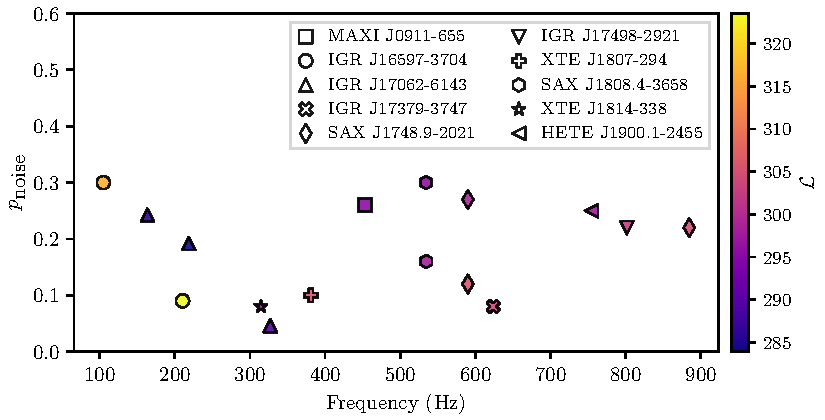
\includegraphics[width=\linewidth]{summary_pnoise.pdf}
	\caption{Summary of search results across all targets and sub-bands with $\ml > \lth$. The different symbols correspond to candidates from different targets. The ordinate shows $\pn$ for each candidate, the probability that a search of that candidate's sub-band in pure noise would return at least one candidate at least as loud as the one seen. The color of each candidate indicates $\mathcal{L}$ (see color bar at right). Candidates that are eliminated by the vetoes outlined in Sec.~\ref{sec:amxp_vetoes} are not shown for clarity. Details on the search results are in Sec.~\ref{sec:amxp_o3results} and Appendix \ref{app:amxp_fullresults}.}
	\label{fig:amxp_summary}
\end{figure*}

In Secs.~\ref{sec:amxp_igrh}--\ref{sec:amxp_hete} we summarize the search results for each of the 20 targets. To guide the reader, and not clutter the main body of the paper, the full search results for one target, \igrh, are shown in Fig.~\ref{fig:amxp_igrh}, while the full search results for the other 19 targets are shown in Figs.~\ref{fig:amxp_igra}--\ref{fig:amxp_hete} in Appendix \ref{app:amxp_fullresults}. The orbital template, terminating frequency bin, $\ml$, and $\pn$ for all 16 candidates with $\ml > \lth$ are collated in Table \ref{tab:outliers} in Appendix \ref{app:amxp_fullresults}. We present further follow-up of the 16 candidates in Appendix \ref{app:amxp_followup}. We find no convincing evidence that any are a true astrophysical signal.

\subsection{IGR J18245--2452  \label{sec:amxp_igrh} }
\begin{figure*}
	\centering
	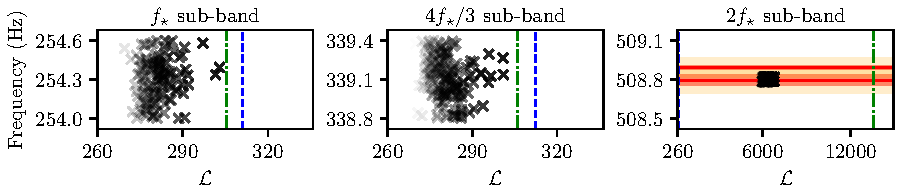
\includegraphics[width=\linewidth]{igr18245.pdf}
	\caption{Search results for \igrh. Black crosses indicate the terminating frequency and $\ml$ for the most likely path through the sub-band for each binary template. The vertical blue dashed (green dot-dashed) lines correspond to the threshold set via Gaussian (off-target) noise realizations, $\lthg$ ($\lthot$), in each sub-band. Solid red lines in the right panel indicate the peak frequency of known instrumental lines in the Hanford detector; the orange band indicates the width of the line in the detector frame and the yellow band indicates the increased effective width due to Doppler broadening, as described in Sec.~\ref{sec:amxp_line_veto}. Multiple overlapping orange bands creates the red bands. The sub-band around $508.8\,$Hz is especially noisy due to test mass suspension violin mode resonances \cite{o23DetChar}. The transparency of crosses in sub-bands with many templates, is adjusted relative to the maximum $\ml$ in that sub-band for clarity.}
	\label{fig:amxp_igrh}	
\end{figure*}
The search results for \igrh\ are presented in Fig.~\ref{fig:amxp_igrh}. Each marker in Fig.~\ref{fig:amxp_igrh} shows the terminating frequency and associated $\ml$ of the most likely path through the sub-band for a given template, i.e.~choice of $P$ and $\tasc$. The vertical blue dashed (green dot-dashed) lines correspond to the threshold set via Gaussian (off-target) noise realizations, $\lthg$ ($\lthot$), in each sub-band, with $\alpha_{N_{\rm tot}} = 0.3$. See Appendix \ref{app:amxp_thresh} for details on how we set thresholds in each sub-band. The horizontal red lines indicate known instrumental lines in the detector with bandwidth indicated by the shading. There are zero above-threshold candidates in the $f_\star$ and $4f_\star / 3$ sub-bands. There are 435 above-threshold candidates in the $2f_\star$ sub-band, which are all coincident with known noise lines in both the Livingston and Hanford detectors, and are therefore eliminated by veto A. The sub-band around $508\,$Hz is especially noisy due to violin mode resonances \cite{o23DetChar}.

\subsection{IGR J00291+5934  \label{sec:amxp_igra} }
The search results for \igra\ are shown in Fig.~\ref{fig:amxp_igra}, which is laid out identically to Fig.~\ref{fig:amxp_igrh}. There are zero above-threshold candidates in the $4f_\star / 3$ and $2f_\star$ sub-bands. There are three above-threshold candidates in the $f_\star$ sub-band, however all three of these candidates are coincident with known noise lines in the Hanford detector, and are therefore eliminated with veto A.

\subsection{MAXI J0911--655  \label{sec:amxp_maxi} }
The search results for \maxi\ are shown in Fig.~\ref{fig:amxp_maxi}, which is laid out identically to Fig.~\ref{fig:amxp_igrh}. There are zero above-threshold candidates in the $f_\star$ and $2f_\star$ sub-bands. There is one above-threshold candidate in the $4f_\star / 3$ sub-band which survives all of the vetoes and has $\pn=0.26$. Additional follow-up, presented in Appendix \ref{app:amxp_followup}, does not provide any evidence that this candidate is a true astrophysical signal.

\subsection{XTE J0929--314  \label{sec:amxp_xtea} }
The search results for \xtea\ are shown in Fig.~\ref{fig:amxp_xtea}, which is laid out identically to Fig.~\ref{fig:amxp_igrh}. There are zero above-threshold candidates across all three sub-bands.

\subsection{IGR J16597--3704  \label{sec:amxp_igrb} }
The search results for \igrb\ are shown in Fig.~\ref{fig:amxp_igrb}, which is laid out identically to Fig.~\ref{fig:amxp_igrh}. Each sub-band for this target is contaminated with known noise lines. There are 84 above-threshold candidates in the $4f_\star / 3$ sub-band, however they are all eliminated by veto B. One above-threshold candidate is returned in each of the $f_\star$ and $2f_\star$ sub-bands. Both of these candidates survive all of the vetoes, and have $\pn=0.30$ and $\pn=0.09$ respectively. Further follow-up, including the frequency path and cumulative log-likelihood for the latter candidate, is presented in Appendix \ref{app:amxp_followup}. This follow-up does not provide any evidence that either candidate is a true astrophysical signal.

\subsection{IGR J17062--6143  \label{sec:amxp_igrc} }
The search results for \igrc\ are shown in Fig.~\ref{fig:amxp_igrc}, which is laid out identically to Fig.~\ref{fig:amxp_igrh}. Given the long-term timing presented in \citet{Bult2021} there is only one template needed in each of the three sub-bands for this target. The template returns $\ml > \lth$ in all three of the $f_\star$, $4f_\star / 3$, and $2f_\star$ sub-bands. All of these candidates survive all of the vetoes, and have $\pn=0.24$, $\pn=0.19$, and $\pn=0.05$ respectively. Further follow-up, including the frequency path and cumulative log-likelihood for the candidate with $\pn=0.05$, is presented in Appendix \ref{app:amxp_followup}. This follow-up does not provide any evidence that any of the three candidates are a true astrophysical signal.

\subsection{IGR J17379--3747  \label{sec:amxp_igrd} }
The search results for \igrd\ are shown in Fig.~\ref{fig:amxp_igrd}, which is laid out identically to Fig.~\ref{fig:amxp_igrh}. There are zero above-threshold candidates in the $f_\star$ and $2f_\star$ sub-bands. There is one above-threshold candidate in the $4f_\star/3$ sub-band which survives all of the vetoes and has $\pn=0.08$. Further follow-up, including the frequency path and cumulative log-likelihood, for this candidate is presented in Appendix \ref{app:amxp_followup}. This follow-up does not provide any evidence that the candidate is a true astrophysical signal.

\subsection{SAX J1748.9--2021   \label{sec:amxp_saxb} }
The search results for \saxb\ are shown in Fig.~\ref{fig:amxp_saxb}, which is laid out identically to Fig.~\ref{fig:amxp_igrh}. There are zero above-threshold candidates in the $f_\star$ sub-band. There are two above-threshold candidates in the $4 f_\star / 3$ sub-band which survive all of the vetoes and have $\pn=0.12$ and $\pn=0.27$. There is one above-threshold candidate in the $2 f_\star$ sub-band which survives all of the vetoes and has $\pn=0.22$. Additional follow-up, presented in Appendix \ref{app:amxp_followup}, does not provide any evidence that any of the three candidates are a true astrophysical signal.

\subsection{NGC 6440 X--2   \label{sec:amxp_ngc} }
The search results for \ngc\ are shown in Fig.~\ref{fig:amxp_ngc}, which is laid out identically to Fig.~\ref{fig:amxp_igrh}. There are zero above-threshold candidates across all three sub-bands.

\subsection{IGR J17494--3030  \label{sec:amxp_igri} }
The search results for \igri\ are shown in Fig.~\ref{fig:amxp_igri}, which is laid out identically to Fig.~\ref{fig:amxp_igrh}. There are zero above-threshold candidates in the $f_\star$ and $2f_\star$ sub-bands. All 4050 candidates in the $4f_\star/3$ sub-band are above threshold, however all of them are coincident with a known noise line in the Hanford detector, and are therefore eliminated with veto A. The sub-band around $501.7\,$Hz is especially noisy due to violin mode resonances \cite{o23DetChar}.

\subsection{Swift J1749.4--2807 \label{sec:amxp_swiftb} }
The search results for \swiftb\ are shown in Fig.~\ref{fig:amxp_swiftb}, which is laid out identically to Fig.~\ref{fig:amxp_igrh}. There are zero above-threshold candidates in the $f_\star$ and $4f_\star / 3$ sub-bands. There is one above threshold candidate in the $2 f_\star$ sub-band. However it is coincident with a known noise line in the Hanford detector, and is therefore eliminated by veto A.

\subsection{IGR J17498--2921  \label{sec:amxp_igre} }
The search results for \igre\ are shown in Fig.~\ref{fig:amxp_igre}, which is laid out identically to Fig.~\ref{fig:amxp_igrh}. There are zero above-threshold candidates in the $f_\star$, and $4f_\star / 3$ sub-bands. There is one above-threshold candidate in the $2f_\star$ sub-band which survives all of the vetoes and has $\pn=0.22$. Additional follow-up, presented in Appendix \ref{app:amxp_followup}, does not provide any evidence that this candidate is a true astrophysical signal.

\subsection{IGR J17511--3057  \label{sec:amxp_igrf} }
The search results for \igrf\ are shown in Fig.~\ref{fig:amxp_igrf}, which is laid out identically to Fig.~\ref{fig:amxp_igrh}. There are zero above-threshold candidates across all three sub-bands.

\subsection{XTE J1751--305  \label{sec:amxp_xteb} }
The search results for \xteb\ are shown in Fig.~\ref{fig:amxp_xteb}, which is laid out identically to Fig.~\ref{fig:amxp_igrh}. There are zero above-threshold candidates across all three sub-bands.

\subsection{Swift J1756.9--2508 \label{sec:amxp_swift} }
The search results for \swift\ are shown in Fig.~\ref{fig:amxp_swift}, which is laid out identically to Fig.~\ref{fig:amxp_igrh}. There are zero above-threshold candidates across all three sub-bands.

\subsection{IGR J17591--2342  \label{sec:amxp_igrg} }
The search results for \igrg\ are shown in Fig.~\ref{fig:amxp_igrg}, which is laid out identically to Fig.~\ref{fig:amxp_igrh}. There are zero above-threshold candidates across all three sub-bands.

\subsection{XTE J1807--294  \label{sec:amxp_xtec} }
The search results for \xtec\ are shown in Fig.~\ref{fig:amxp_xtec}, which is laid out identically to Fig.~\ref{fig:amxp_igrh}. There are zero above-threshold candidates in the $f_\star$ and $4f_\star / 3$ sub-bands. There is one above-threshold candidate in the $2f_\star$ sub-band which survives all of the vetoes and has $\pn=0.10$. Further follow-up, including the frequency path and cumulative log-likelihood, for this candidate is presented in Appendix \ref{app:amxp_followup}. This follow-up does not provide any evidence that the candidate is a true astrophysical signal.

\subsection{SAX J1808.4--3658   \label{sec:amxp_sax} }
The search results for \sax\ are shown in Fig.~\ref{fig:amxp_sax}, which is laid out identically to Fig.~\ref{fig:amxp_igrh}. There are zero above-threshold candidates in the $f_\star$ and $2f_\star$ sub-bands. There are two above-threshold candidates in the $4f_\star / 3$ sub-band which survive all of the vetoes and have $\pn=0.16$ and $\pn=0.30$. Additional follow-up, presented in Appendix \ref{app:amxp_followup}, does not provide any evidence that either candidate is a true astrophysical signal.

\sax\ was observed in outburst in August 2019, during O3a \cite{Bult2020, Goodwin2020}. This allows us to perform an additional target-of-opportunity search during only its active phase. If the target only emits continuous gravitational waves during outburst, searching a shorter duration of data increases the probability of detection by increasing the signal-to-noise ratio. The details and results of this target-of-opportunity search are in Sec.~\ref{sec:amxp_shortsax}. In summary, after searching with three separate coherence times of $\tdr = 1\,$d, $\tdr=8\,$d, and $\tdr=24\,$d, only one candidate is above threshold and survives all of the vetoes. The candidate is found using $\tdr=24\,$d in the $f_\star$ sub-band, and has $\pn = 0.02$. Additional follow-up does not reveal any informative features that would distinguish between an astrophysical signal and noise. It does not coincide with either of the two candidates in the $4f_\star / 3$ sub-band found in the semi-coherent search using the full O3 data set. 

\subsection{XTE J1814--338  \label{sec:amxp_xted} }
The search results for \xted\ are shown in Fig.~\ref{fig:amxp_xted}, which is laid out identically to Fig.~\ref{fig:amxp_igrh}. There are zero above-threshold candidates in the $4f_\star / 3$ and $2f_\star$ sub-bands. There is one above-threshold candidate in the $f_\star$ sub-band which survives all of the vetoes and has $\pn=0.08$.  Further follow-up, including the frequency path and cumulative log-likelihood, for this candidate is presented in Appendix \ref{app:amxp_followup}. This follow-up does not provide any evidence that the candidate is a true astrophysical signal.

\subsection{HETE J1900.1--2455  \label{sec:amxp_hete} }
The search results for \hete\ are shown in Fig.~\ref{fig:amxp_hete}, which is laid out identically to Fig.~\ref{fig:amxp_igrh}. There are zero above-threshold candidates in the $f_\star$ sub-band. All 22 templates in the $4f_\star / 3$ sub-band return candidates above $\lth$, however these candidates are all coincident with known noise lines in the Hanford detector, and are summarily eliminated with veto A. The sub-band around $503\,$Hz is especially noisy due to violin mode resonances \cite{o23DetChar}. There is one above-threshold candidate in the $2f_\star$ sub-band which survives all of the vetoes and has $\pn=0.25$. Additional follow-up, presented in Appendix \ref{app:amxp_followup}, does not provide any evidence that this candidate is a true astrophysical signal.

\section{Target-of-opportunity search: SAX J1808.4--3658 in outburst \label{sec:amxp_shortsax}}
On August 7 2019 \sax\ went into outburst \cite{Bult2019}. The Neutron star Interior Composition Explorer (NICER) team undertook a high-cadence monitoring campaign, and performed a timing analysis of the pulsations \cite{Bult2020}. The outburst lasted for roughly 24 days, with enhanced X-ray flux observed between August 7 2019 and August 31 2019 (see Fig.~1 of \citet{Bult2020}). We note that the \emph{Swift} X-ray Telescope observed increased X-ray activity from August 6 2019, and observations in the optical $i'$-band with the Las Cumbres Observatory network detected an increased flux from July 25 2019 \cite{Goodwin2020}.

Outburst events are attributed to in-falling plasma that is channeled by the magnetosphere onto a localized region on the neutron star surface, creating a hot spot that rotates with the star \cite{Romanova2004}. As the observed X-ray flux is assumed to be linearly proportional to the mass accretion rate, an outburst could result in a larger mountain on the neutron star surface (or excite $r$-modes in the interior), compared to when the AMXP is in quiescence \cite{Haskell2015GW, Haskell2017a}. 

If continuous gravitational waves are only emitted from \sax\ when it is in outburst, searching all of the O3 data decreases the signal-to-noise ratio, as compared to only searching data from the outburst. To protect against this possibility, we do an additional search for continuous gravitational waves from \sax\ using data from both LIGO observatories between 1249171218 GPS time (August 7 2019) and 1251244818 GPS time (August 31 2019), rather than data from the entirety of O3, as in Sec.~\ref{sec:amxp_sax}. 

\subsection{Search parameters}
The search algorithm is laid out in Sec.~\ref{sec:amxp_alg}. We run the search using three different coherence times, setting $\tdr = 1\,$d, $\tdr = 8\,$d, and $\tdr = 24\,$d. We search three sub-bands centered on $\{1, 4/3, 2\}f_\star$, for each $\tdr$. The width of the sub-band depends on $\tdr$. It is $\sim 0.76\,$Hz for the searches with $\tdr=1\,$d and $8\,$d, and is $\sim 1.01\,$Hz for the search with $\tdr=24\,$d. Given the precise timing achieved during the outburst in 2019 \cite{Bult2020}, and the shorter search duration, only one $\{P,\ \tasc,\ a_0\}$ template is required for each sub-band, according to Eqs.~\eqref{eq:amxp_np}--\eqref{eq:amxp_ntasc}. Due to the different values of $\tdr$, shorter total duration, and different number of templates, we re-calculate $\lth$ for each sub-band and value of $\tdr$, using the procedure outlined in Sec.~\ref{sec:amxp_thresh} and Appendix \ref{app:amxp_thresh}. As in the full O3 search, we set the probability of false alarm in each sub-band at $\alpha_{N_{\rm tot}} = 0.3$. For all candidates that have $\ml > \lth$ we apply the three vetoes described in \ref{sec:amxp_vetoes}.

\subsection{Search results}
For $\tdr = 1\,$d, the search in the $f_\star$ sub-band returns one candidate above $\lth$. The candidate survives both veto A (known line) and veto B (single interferometer), but fails veto C (off-target). The searches in the $4/3f_\star$ and $2f_\star$ sub-bands do not return any candidates above $\lth$.

For $\tdr = 8\,$d, there are no candidates above $\lth$ in any of the three sub-bands.

For $\tdr = 24\,$d, the searches in the $4 f_\star /3$ and $2f_\star$ sub-bands do not return any candidates above $\lth$. The search in the $f_\star$ sub-band does return one candidate above $\lth$. This candidate survives all of the vetoes outlined in Sec.~\ref{sec:amxp_vetoes}. We remind the reader that with $\alpha_{N_{\rm tot}} = 0.3$ and nine sub-bands searched (three for each of the three choices of $\tdr$), we should expect $\sim 3$ candidates above threshold purely due to noise. The probability that we would see a value of $\ml$ at least this large if this sub-band is pure noise, $\pn$, is 0.02. The template and frequency of the candidate are not coincident with any candidate from the full O3 search (see Table \ref{tab:outliers}) or the sub-threshold candidate found in the search of this sub-band in O2 data \cite{Middleton2020}. By setting $\tdr = T_{\rm obs} = 24\,$d we perform a fully coherent search across this time period, with a frequency bin size of $\Delta f = 2.4\times10^{-7}\,$Hz. We describe in Appendix \ref{app:amxp_shortsax_followup} further follow-up of this candidate. In summary, we find no significant evidence that it is an astrophysical signal rather than a noise fluctuation.

\section{Frequentist upper limits \label{sec:amxp_ul}}
If we assume that the remaining candidates reported in Sec.~\ref{sec:amxp_o3results} and Appendix \ref{app:amxp_fullresults} are false alarms, we can place an upper limit on the wave strain that is detectable at a confidence level of 95\%, $\hul$, in a sub-band. The value of $\hul$ is a function of our algorithm, the detector configuration during O3, and our assumptions about the signal model. We describe the method used to estimate $\hul$ in Sec.~\ref{sec:amxp_ul_method}, present the upper limits in each sub-band in Sec.~\ref{sec:amxp_ul_results}, and compare the results to indirect methods that calculate the expected strain in the $2f_\star$ sub-band in Sec.~\ref{sec:amxp_ul_comp}. The astrophysical implications are discussed in Sec.~\ref{sec:amxp_ul_impl}.

\subsection{Upper limit procedure in a sub-band \label{sec:amxp_ul_method}}
We set empirical frequentist upper limits in each sub-band using a sequence of injections into O3 SFTs. For each sub-band we inject $N_{\rm trials}=100$ simulated binary signals at 12--15 fixed values of $h_0$ using \texttt{lalapps\_Makefakedata\_v5} \cite{LAL2018}. For each of the $N_{\rm trials}$ injections at a fixed $h_0$ we select a constant injection frequency, $f_{\rm inj}$, uniformly from the sub-band. While the injected signal has zero spin-wandering, we still use $\tdr=10\,$d in the search algorithm outlined in Sec.~\ref{sec:amxp_alg} to mimic the real search. The injected period, $P_{\rm inj}$, and time of ascension, $T_{\rm asc,\,inj}$ are chosen uniformly from the ranges $[P - 3\sigma_P, P + 3\sigma_P]$ and $[\tasc - 3\sigma_{\tasc}, \tasc + 3\sigma_{\tasc}]$ respectively. We keep $a_0$ fixed at the precisely known value for each target. The polarization, $\psi$, is chosen uniformly from the range $[0, 2\pi]$. The cosine of the projected inclination angle of the neutron star spin axis with our line of sight, $\cos\iota$, is chosen uniformly from the range $[-1, 1]$\footnote{While the inclination angle of the binary with respect to our line of sight is restricted via EM observations for some of our targets, we opt to marginalize over $\cos\iota$ as the neutron star spin axis may not necessarily align with the orbital axis of the binary. It is possible to scale our results via equation (19) of \citet{Messenger2015a}, if one wishes to fix $\cos\iota$.}. We then search for the injected signal with the template in this sub-band's template grid that is nearest to $\{P_{\rm inj}, T_{\rm asc,\,inj}\}$. We re-calculate $\lth$ such that the probability of false alarm in each sub-band is $\alpha_{N_{\rm tot}} = 0.01$. This allows us to set conservative upper limits, even in sub-bands where we have marginal candidates above a threshold corresponding to a probability of false alarm of 30\% per sub-band. By recording the fraction of injected signals we recover at each $h_0$ with $\ml > \lth$ we estimate the efficiency, $\varepsilon$, as a function of $h_0$. We then perform a logistic regression \cite{Gelman2013} to obtain a sigmoid fit to $\varepsilon(h_0)$, and solve 
\begin{equation}
\varepsilon(\hul) = 0.95\ , \label{eq:amxp_effic_95}
\end{equation}
to find an estimate of $\hul$ in the given sub-band. 

One might reasonably ask, how precise is this estimate of $\hul$? The main factors impacting the precision are: \begin{enumerate*}
\item the precision of the most likely parameters of the sigmoid, as estimated via logistic regression, when solving Eq.~\eqref{eq:amxp_effic_95} for $\hul$, given the $N_{\rm trials}$ injections done at 12--15 values of $h_0$; and
\item the assumption that the strain data (and hence the SFTs) are perfectly calibrated.
\end{enumerate*}
We investigate the impact of (i) by drawing alternative sigmoid fits of $\varepsilon(h_0)$ using the covariance matrix of the parameters returned by the logistic regression. We find that inverting these alternative fits through Eq.~\eqref{eq:amxp_effic_95} results in a value of $\hul$ that varies by less than $5\%$ from the value calculated via the most likely parameters (at the 95\% confidence level). The impact of (ii) is trickier to quantify. As described in \citet{Sun2020, Sun2021} the median systematic error in the magnitude of the strain is less than $2\%$ in the 20--2000\,Hz frequency band across O3a. The statistical uncertainty around the measurement of calibration bias means that in the worst case the true magnitude of the calibration bias may be as large as $7\%$. However, the calibration bias at a given frequency is not correlated between the detectors (see Figures 16 and 17 in \citet{Sun2020}), and so the impact on a continuous gravitational wave search that combines data from both detectors is likely to be less than $7\%$. 

In light of the above considerations we quote $\hul$ to a precision of two significant figures, but we emphasize that estimating $\hul$ involves many (potentially compounding) uncertainties. Subsequent conclusions about the physical system that are drawn from estimates of $\hul$ cannot be more precise than the estimate of $\hul$ itself.

\subsection{Upper limits \label{sec:amxp_ul_results}}
The estimates of $\hul$ for each target and sub-band are listed in Table \ref{tab:ul}. Dashes correspond to sub-bands that are highly contaminated with noise lines, which preclude the procedure described in Sec.~\ref{sec:amxp_ul_method}, as one always finds $\ml > \lth$, regardless of $h_0$. The most sensitive sub-bands are for IGR J17062$-$6143 with $\hul = 4.7 \times 10^{-26}$ in both the $4f_\star/3$ and $2f_\star$ sub-bands (centered around 218.2\,Hz and 327.6\,Hz respectively). These sub-bands lie in the most sensitive band of the detector, and the binary elements are known to high precision \cite{Bult2021}, so only one template is needed in each sub-band, corresponding to a relatively lower $\lth$ at fixed probability of false alarm.

No estimates of $\hul$ were established in \citet{Middleton2020} for the five targets therein. The search of XTE J1751$-$305 in S6 data estimated $\hul \approx 3.3\times10^{-24}$, $4.7\times10^{-24}$, and $7.8\times10^{-24}$ in three sub-bands corresponding to $f_\star$, an $r$-mode frequency, and $2f_\star$ respectively \cite{s6twoSpectScoXTE}. Our estimates of $\hul$ for XTE J1751$-$305 improve these results by two orders of magnitude, because the detector is more sensitive, and $\tdr$ is longer.

\begin{table}
\centering
\caption{Upper limits on the detectable gravitational wave strain at a 95\% confidence level, $\hul$, in each of the sub-bands for each target. See Sec.~\ref{sec:amxp_ul_method} for details on how they are estimated, and the precision to which they are known. Upper limits are not estimated in sub-bands marked with a ``$-$'' as these sub-bands are highly contaminated with known noise lines. \label{tab:ul}}
\resizebox{0.7\textwidth}{!}{%
\begin{tabular}{l d{5} d{5} d{5}}
\toprule
	& \multicolumn{3}{c}{\textrm{$\hul$ in each sub-band ($\times 10^{-26}$)}} \\
\textrm{Target}	& \textrm{$f_{\rm \star}$} & \textrm{$4f_{\rm \star}/3$} & \textrm{$2f_{\rm \star}$}  \\
\midrule
IGR J00291$+$5934      & -  	    & 7.6     	& 11    \\
MAXI J0911$-$655       & 7.7  	    & 6.4     	& 7.3   \\
XTE J0929$-$314        & 5.1  	    & 5.3       & 6.4   \\
IGR J16597$-$3704      & 7.5  	    & - 		& 5.6   \\
IGR J17062$-$6143      & 8.1  	    & 4.7   	& 4.7   \\
IGR J17379$-$3747      & 8.5  	    & 7.4   	& 10    \\
SAX J1748.9$-$2021     & 9.2  	    & 7.7   	& 10  \\
NGC 6440 X$-$2         & 6.2  	    & 7.2     	& 5.8   \\
IGR J17494$-$3030	   & 8.3  	    & - 		& 9.0   \\
Swift J1749.4$-$2807   & 11 	    & 17  		& 24    \\
IGR J17498$-$2921      & 7.0  	    & 6.6       & 8.4   \\
IGR J17511$-$3057      & 7.5  	    & 5.5       & 6.6   \\
XTE J1751$-$305        & 10 	    & 8.3       & 9.7   \\
Swift J1756.9$-$2508   & 8.1  	    & 8.8     	& 6.3   \\
IGR J17591$-$2342      & 9.5  	    & 11   	    & 14    \\
XTE J1807$-$294        & 6.1  	    & 5.0       & 5.6   \\
SAX J1808.4$-$3658     & 6.4        & 6.9       & 8.8   \\
XTE J1814$-$338        & 9.4  	    & 6.0       & 6.9   \\
IGR J18245$-$2452      & 9.0  	    & 6.3       & - 	\\
HETE J1900.1$-$2455    & 5.6    	& -	        & 8.4   \\
\bottomrule
\end{tabular}
}
\end{table}

\subsection{Comparison to expected strain from AMXPs \label{sec:amxp_ul_comp}}
It is valuable to consider how strong the signal from our targets could be, given EM observations. If we assume that all rotational energy losses, as observed in the frequency derivative $\dot{f}_\star$, are converted into gravitational radiation, the indirect spin-down limit on the maximum strain, $h_{0,\,\textrm{sd}}$, is \cite{Riles2013a}
\begin{align}
h_{0,\,\textrm{sd}} = &~4.0\times 10^{-28} \left( \frac{8\,{\rm kpc}}{D}\right) \nonumber \\
					&\times \left(\frac{600\,{\rm Hz}}{f_{\rm GW}} \right)^{1/2} \left(\frac{-\dot{f}_{\rm GW}}{10^{-14}\,{\rm Hz\,s}^{-1}} \right)^{1/2}\ , \label{eq:amxp_h0sd}
\end{align}
where $D$ is the distance to the target, $f_{\rm GW}$ is the gravitational wave frequency, and $\dot{f}_{\rm GW}$ is its derivative. In Eq.~\eqref{eq:amxp_h0sd} we assume $I_{zz} / I_0 \approx 1$, i.e.~the $zz$ component of the moment-of-inertia tensor ($I_{zz}$) is very close to the moment-of-inertia of an undeformed star ($I_0$). We assume $f_{\rm GW} \approx 2 f_\star$ when computing Eq.~\eqref{eq:amxp_h0sd} for each of our targets. We list the best estimates for the distance to each target in the second column of Table \ref{tab:exp_ul}. These estimates are typically poorly known, especially if there is no known counterpart observed in wavelengths other than X-ray for the target. We use the central estimate of the distance in Eq.~\eqref{eq:amxp_h0sd}.

For AMXPs, $\dot{f}_\star$ is estimated by constructing a phase-connected timing solution when the target is in outburst, but estimates for $\dot{f}_\star$ in quiescence are also possible for targets that have gone into outburst multiple times. The $\dot{f}_\star$ observed during outburst can be either positive (corresponding to spin-up) or negative (corresponding to spin-down), while in quiescence $\dot{f}_\star$ is typically (but not always) negative \cite{Ghosh1977, Melatos2016}. The third column of Table \ref{tab:exp_ul} records $\dot{f}_\star$ for each of our targets. When $\dot{f}_\star$ has been measured in multiple outburst events, only the $\dot{f}_\star$ from the most recent outburst is listed. For $\dot{f}_\star < 0$ we assume $\dot{f}_\textrm{GW} \approx 2 \dot{f}_\star$ in Eq.~\eqref{eq:amxp_h0sd}. For targets with $\dot{f}_\star < 0$ (in either quiescent or active phases) we find $10^{-28} \lesssim h_{0,\,\textrm{sd}} \lesssim 10^{-27}$ (fourth column of Table \ref{tab:exp_ul}), an order of magnitude lower than the estimated value of $\hul$. 

As argued in \citet{Middleton2020}, for $\dot{f}_\star > 0$ the torque due to gravitational radiation reaction may be masked by the accretion torque, allowing larger values of $\dot{f}_\textrm{GW}$, as long as one has $\dot{f}_\star = \dot{f}_\textrm{acc} + \dot{f}_\textrm{GW}$, where $\dot{f}_\textrm{acc}$ is the spin-up rate due to accretion. A reasonable choice, without excessive fine-tuning, is to set $\dot{f}_\textrm{GW} \approx - \dot{f}_\star$, for an order-of-magnitude estimate in Eq.~\eqref{eq:amxp_h0sd}, i.e.~assuming $|\dot{f}_\textrm{acc}| \approx 2 |\dot{f}_\textrm{GW}|$. The resultant values for $h_{0,\,\textrm{sd}}$ for targets with $\dot{f}_\star > 0$ are all well below the estimates of $\hul$ set in Sec.~\ref{sec:amxp_ul_results}, and fall in the range $10^{-28} \lesssim h_{0,\,\textrm{sd}} \lesssim 10^{-27}$. 

Another avenue through which EM observations can constrain $h_0$ is by assuming that the X-ray flux is proportional to the mass accretion rate, and that the torque due to accretion balances the gravitational radiation reaction. The torque-balance limit is \cite{Riles2013a, Zhang2021}
\begin{align}
h_{0,\,\textrm{torque}} = &~5\times 10 ^{-27}\left(\frac{600\,\textrm{Hz}}{f_\textrm{GW}}\right)^{1/2} \nonumber \\
						&\times \left(\frac{F_X}{10^{-8}\,\textrm{erg\,s$^{-1}\,$cm$^{-2}$}}\right)^{1/2}\ ,  \label{eq:amxp_h0t}
\end{align}
where $F_X$ is the observed bolometric X-ray flux. Eq.~\eqref{eq:amxp_h0t} has a few hidden assumptions, namely: \begin{enumerate*}
\item that the mass of the neutron star is $1.4M_\odot$,
\item that all of the accretion luminosity is radiated as an X-ray flux, and
\item that the accretion torque is applied at the radius of the neutron star, which is set to 10\,km.
\end{enumerate*}
The exact dependence of the torque-balance limit on these assumptions is discussed in \citet{Zhang2021}. We take $f_{\rm GW} \approx 2 f_\star$ for each of our targets, as for Eq.~\eqref{eq:amxp_h0sd}. We take $F_X = F_{X,\,\textrm{max}}$, the maximum recorded X-ray flux from each target when it was in outburst (fifth column of Table \ref{tab:exp_ul}), providing an upper limit on $h_{0,\,\textrm{torque}}$ (sixth column of Table \ref{tab:exp_ul}). We find $5\times 10^{-28} \lesssim h_{0,\,\textrm{torque}} \lesssim 1\times 10^{-27}$ across all targets. 

\emph{Full caption for Table \ref{tab:exp_ul}:} Maximum expected strain from each target, as inferred from EM observations. The second column contains the best estimate for the distance to the target. Targets with ``-'' listed as the frequency derivative (third column), $\dot{f}_\star$, do not have a measured value during outburst, and also do not have a long-term (quiescent) $\dot{f}_\star$ measured either. The labels (A) and (Q) indicate that $\dot{f}_\star$ is measured in outburst and quiescence respectively. The scaling equations used to estimate the maximum spin-down strain (fourth column), $h_{0,\,\textrm{sd}}$, and the maximum strain assuming torque-balance (sixth column), $h_{0\,\textrm{torque}}$, are Eqs.~\eqref{eq:amxp_h0sd} and \eqref{eq:amxp_h0t} respectively. The $h_{0,\,\textrm{sd}}$ value is calculated using the central distance and $\dot{f}_\star$ estimates. The $h_{0\,\textrm{torque}}$ value is calculated using the maximum bolometric X-ray flux measured during outburst (fifth column), $F_{X,\,\textrm{max}}$, which is typically measured to a precision of $\sim10\%$. The X-ray flux of each target in quiescence is not shown, as it is only measured for half of the targets, and is usually $\sim1-2$ orders of magnitude lower than $F_{X,\,\textrm{max}}$. The seventh column contains $\hul$ in the $2f_\star$ sub-band (fourth column of Table \ref{tab:ul}) to facilitate comparisons between $\hul$ and $h_{0\,\textrm{torque}}$ or $h_{0,\,\textrm{sd}}$.

\begin{landscape}
\begin{table}
\caption{Full caption on previous page. \label{tab:exp_ul}}
\resizebox{1.5\textwidth}{!}{%
\NiceMatrixOptions{notes/para}
\begin{NiceTabular}{l r r r r r r l}
\toprule
	& \textrm{Distance} &	 & \textrm{$h_{0,\,\textrm{sd}}$} & \textrm{$F_{X,\,\textrm{max}}$ $(\times 10^{-8}$} & \textrm{$h_{0,\textrm{torque}}$} & \textrm{$\hul$} & \\
Target & \textrm{(kpc)} & \textrm{$\dot{f}_\star$ (Hz\,s$^{-1}$)}  & \textrm{$(\times 10^{-26})$} & \textrm{erg\,s$^{-1}\,$cm$^{-2}$)} & \textrm{$(\times 10^{-26})$} & \textrm{$(\times 10^{-26})$} & \textrm{Refs.} \\
\midrule
IGR J00291$+$5934   	& \textrm{4.2(5)} 		 & $-4.0(1.4)\times 10^{-15}$  (Q)				& 0.05 			& 0.35  	& 0.2   & 11   &\cite{Watts2008, Papitto2011, Sanna2017, DeFalco2017} \\
MAXI J0911$-$655    	& \textrm{9.45(15)} 	 & -	  										& -				& 0.047  	& 0.1   & 7.3  &\cite{Watkins2015, Homan2016, Sanna0911} \\
XTE J0929$-$314     	& \textrm{7.4\tabularnote{Estimate assumes conservative mass transfer during accretion. An alternative estimate gives less than $4\,$kpc \cite{Marino2017}.}}  & $-9.2(4)\times 10^{-14}$  (A)  				& 0.2			& 0.1  		& 0.2   & 6.4  &\cite{Galloway2002, Watts2008, Marino2017} \\
IGR J16597$-$3704   	& \textrm{9.1\tabularnote{Uncertainty not quoted as target located in a globular cluster.}}  & -  						   	  				& -				& 0.065  	& 0.2   & 5.6  &\cite{Sanna16597} \\
IGR J17062$-$6143   	& \textrm{7.3(5)} 		 & $+3.77(9)\times 10^{-15}$ (A)  				& 0.04\tabularnote{Assumes $\dot{f}_\textrm{GW} \approx - \dot{f}_\star$, see text for details.}	& 0.006  	& 0.05  & 4.7  &\cite{Keek2017, Bult2021} \\
IGR J17379$-$3747   	& \textrm{8\tabularnote{Unknown, but as the target is in the direction of the galactic centre a fiducial value of 8\,kpc is assumed in the literature.}} 	 & $-1.2(1.9)\times 10^{-14}$\tabularnote{Estimate of $\dot{f}_\star$ consistent with zero at a $3\sigma$ level.} (A)		& 0.05			& 0.04  	& 0.08  & 10   &\cite{VanDenEijnden2018a, Negoro2018, Sanna17379, Bult17379} \\
SAX J1748.9$-$2021  	& \textrm{8.5\tabularnote{Uncertainty not quoted as target located in a globular cluster.}}  & -										  	& -				& 0.077  	& 0.1   & 10   &\cite{Watts2008, Harris2010, Sanna1748, Sharma2020} \\
NGC 6440 X$-$2      	& \textrm{8.5\tabularnote{Uncertainty not quoted as target located in a globular cluster.}}  & -  						   			    	& -				& 0.02  	& 0.09  & 5.8  &\cite{Harris2010, Bult2015} \\
IGR J17494$-$3030     	& \textrm{8\tabularnote{Unknown, but as the target is in the direction of the galactic centre a fiducial value of 8\,kpc is assumed in the literature.}} 	 & $-2.1(7)\times 10^{-14} $ (Q)  				& 0.07			& 0.0143  	& 0.05  & 9.0  &\cite{Ng2021} \\
Swift J1749.4$-$2807	& \textrm{6.7(1.3)} 	 & -  						   			    	& -				& 0.0352  	& 0.07  & 24   &\cite{Wijnands2009, Bult2021a, Sanna2022} \\
IGR J17498$-$2921   	& \textrm{7.6(1.1)}  	 & $-6.3(1.9)\times 10^{-14}\ \tabularnote{Estimate of $\dot{f}_\star$ consistent with zero at a $3\sigma$ level.}\ $ (A) 	& 0.1 			& 0.2  		& 0.2   & 8.4  &\cite{Linares2011, Papitto17498, Falanga2012} \\
IGR J17511$-$3057   	& \textrm{3.6(5)} 		 & $+4.8(1.4)\times 10^{-14} $ (A)  			& 0.2\tabularnote{Assumes $\dot{f}_\textrm{GW} \approx - \dot{f}_\star$, see text for details.}	& 0.2  		& 0.2   & 6.6  &\cite{Riggio17511} \\
XTE J1751$-$305     	& \textrm{6.7\tabularnote{Lower limit.}}  & $-5.5(1.2)\times 10^{-15}$  (Q)  			& 0.04			& 0.29  	& 0.2   & 9.7  &\cite{Watts2008, Papitto1751, Riggio2011} \\
						& 						 & $+3.7(1.0)\times 10^{-13}$  (A)  			& 0.2\tabularnote{Assumes $\dot{f}_\textrm{GW} \approx - \dot{f}_\star$, see text for details.}	& 		  	& 	    &      & \\
Swift J1756.9$-$2508	& \textrm{8\tabularnote{Unknown, but as the target is in the direction of the galactic centre a fiducial value of 8\,kpc is assumed in the literature.}} 	 & $-4.8(6)\times 10^{-16}$  (Q)  				& 0.02			& 0.288  	& 0.3   & 6.3  &\cite{Watts2008, Sanna1756} \\
						& 					 	 & $-4.3(2.1)\times 10^{-11}$\ \tabularnote{Estimate of $\dot{f}_\star$ consistent with zero at a $3\sigma$ level.}\ \ (A) & 5				& 		  	& 	    &      & \\
IGR J17591$-$2342   	& \textrm{7.6(7)} 		 & $-7.1(4)\times 10^{-14} $ (A)  				& 0.1			& 0.0535  	& 0.09  & 14   &\cite{Gusinskaia2020, Kuiper2020, Sanna17591} \\
XTE J1807$-$294     	& \textrm{8\tabularnote{Unknown, but as the target is in the direction of the galactic centre a fiducial value of 8\,kpc is assumed in the literature.}} 	 & $+2.7(1.0)\times 10^{-14}$  (A)  			& 0.08\tabularnote{Assumes $\dot{f}_\textrm{GW} \approx - \dot{f}_\star$, see text for details.}	& 0.2  		& 0.3   & 8.8  &\cite{Watts2008, Riggio2008, Patruno1807} \\
SAX J1808.4$-$3658  	& \textrm{$3.3^{+0.3}_{-0.2}$} & $-1.01(7)\times 10^{-15}$ (Q)  		& 0.04			& 0.103  	& 0.1   & 5.6  &\cite{Galloway2006, Watts2008, Goodwin2019, Bult2020} \\
						& 				 		 & $-3.02(13)\times 10^{-13}$ (A) & 0.7			& 		  	& 	    & 	   & \\
XTE J1814$-$338     	& \textrm{10.25(1)} 	 & $-6.7(7)\times 10^{-14}$  (A)  				& 0.1			& 0.069  	& 0.1   & 6.9  &\cite{Papitto1814, Watts2008, DAvanzo2009} \\
IGR J18245$-$2452   	& \textrm{5.5\tabularnote{Uncertainty not quoted as target located in a globular cluster.}}  & -  						   			    	& -				& 0.0466  	& 0.1   & -    &\cite{Harris2010, Papitto18245, Campana2018} \\
HETE J1900.1$-$2455 	& \textrm{4.5(2)} 		 & $+4.2(1)\times 10^{-13}$  (A)  				& 0.4\tabularnote{Assumes $\dot{f}_\textrm{GW} \approx - \dot{f}_\star$, see text for details.}	& 0.09  	& 0.1   & 8.4  &\cite{Suzuki2007, Galloway2008, Patruno1900, Watts2008} \\
\bottomrule
\end{NiceTabular}
}
\end{table}
\end{landscape}

\subsection{Astrophysical implications \label{sec:amxp_ul_impl}}

\begin{figure*}
	\centering
	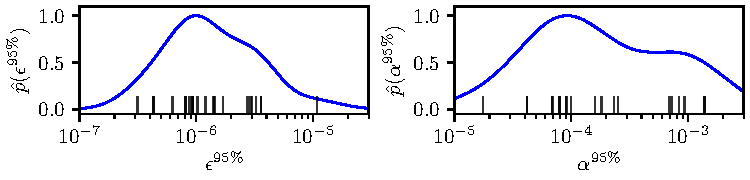
\includegraphics[width=\linewidth]{kde.pdf}
	\caption{Kernel density estimate of the PDF of the constraints on ellipticity $\epsilon^{95\%}$ (left panel) and dimensionless $r$-mode amplitude $\alpha^{95\%}$ (right panel) via Eqs.~\eqref{eq:amxp_ellip} and \eqref{eq:amxp_alpha} respectively. Both PDFs are normalized to a height of one. The black dashes in both panels correspond to the individual estimates of $\epsilon^{95\%}$ or $\alpha^{95\%}$ from each target.}
	\label{fig:amxp_kde}
\end{figure*}

The estimates of $\hul$ given in Sec.~\ref{sec:amxp_ul_results} can be converted into constraints on the physical parameters that govern the mechanism putatively generating continuous gravitational waves in each sub-band.

In the $2f_\star$ sub-band the simplest emission mechanism is that of a perpendicular biaxial rotator (using the language from \citet{Sun2019}), for which we calculate the upper limit of the ellipticity of the neutron star as \cite{JKS98}
\begin{equation}
\epsilon^{95\%} = 2.1 \times 10^{-6} \left(\frac{\hul}{10^{-25}} \right) \left(\frac{D}{8\,\textrm{kpc}} \right) \left(\frac{600\,\textrm{Hz}}{f_{\textrm{GW}}} \right)^2\ , \label{eq:amxp_ellip}
\end{equation}
assuming $I_{zz} = 10^{38}\,$kg\,m$^2$. Using the central estimate for $D$ (second column of Table \ref{tab:exp_ul}), we find the strictest constraint, from all of our targets, $\epsilon^{95\%} = 3.1\times 10^{-7}$ for IGR J00291$+$5934. A kernel density estimate of the probability density function (PDF) of the constraints $\epsilon^{95\%}$, $\hat{p}(\epsilon^{95\%})$, for all our targets, is shown in the left panel of Fig.~\ref{fig:amxp_kde}. It is peaked around $\epsilon^{95\%} \sim 10^{-6}$. 

In the $4f_\star/3$ sub-band the emission mechanism is via $r$-modes, the strength of which is parametrized as \cite{Owen2010}
\begin{equation}
\alpha^{95\%} = 1.0\times10^{-4} \left(\frac{\hul}{10^{-25}} \right) \left(\frac{D}{8\,\textrm{kpc}} \right) \left(\frac{600\,\textrm{Hz}}{f_{\textrm{GW}}} \right)^3\ . \label{eq:amxp_alpha}
\end{equation}
Eq.~\eqref{eq:amxp_alpha} assumes $f_{\textrm{GW}} \approx 4f_\star/3$, which may not be true, as discussed in Sec.~\ref{sec:amxp_params} \cite{Idrisy2015, Caride2019}. The strictest constraint, from all of our targets, is $\alpha^{95\%} = 1.8\times 10^{-5}$, again for IGR J00291$+$5934. A kernel density estimate of the PDF of the constraints $\alpha^{95\%}$, $\hat{p}(\alpha^{95\%})$, for all our targets, is shown in the right panel of Fig.~\ref{fig:amxp_kde}. It is peaked around $\alpha^{95\%} \sim 10^{-4}$.

The kernel density estimates of the PDFs $\hat{p}(\epsilon^{95\%})$ and $\hat{p}(\alpha^{95\%})$ in Fig.~\ref{fig:amxp_kde} are not constraints on $\epsilon$ and $\alpha$ respectively, nor are they expressing the uncertainty in each individual estimate of $\epsilon^{95\%}$ or $\alpha^{95\%}$ (which are dominated by the uncertainty in $\hul$, and the distance, see column two of Table~\ref{tab:exp_ul}). They are instead presented to indicate where the constraints on $\epsilon^{95\%}$ and $\alpha^{95\%}$ lie, given the strain upper limits calculated for the targets in this search. That is, they are estimates of the true probability distribution of the constraints one would obtain for $\epsilon$ and $\alpha$, given a large population of AMXPs (assuming the targets studied here are representative of this larger population). The kernel density estimates are calculated by summing Gaussian kernels centered on each data point, with bandwidth chosen to minimize the asymptotic mean integrated square error \cite{Wand1995}.

The physical mechanism for emission in the $f_\star$ sub-band is less well-defined. A biaxial non-perpendicular rotator emits gravitational radiation at both $f_\star$ and $2f_\star$ \cite{JKS98, Jones2010, Jones2015}. The emission at $f_\star$ dominates the $2f_\star$ emission for both $\theta \lesssim 20\degr$ and $|\cos\iota| \lesssim 0.8$, where $\theta$ is the wobble angle (see figure 5 of \citet{Sun2019} for details). The value of $\theta$ is low for certain models involving pinned superfluid interiors \cite{Jones2010, Melatos2015}. Other possibilities exist, including a triaxial rotator \cite{Zimmermann1980, Broeck2005, Lasky2013}. We recommend future searches to also consider searching the $f_\star$ sub-band, due to the wealth of information that a continuous gravitational wave detection at this frequency would provide regarding neutron star structure.

\section{Conclusions} \label{sec:amxp_concl}
We present the results of a search for continuous gravitational waves from 20 accreting low-mass X-ray binaries in the Advanced LIGO O3 dataset. Five of these targets were searched before in O2 \cite{Middleton2020}, and one was searched in S6 \cite{s6twoSpectScoXTE}. The search pipeline we use allows for spin-wandering and tracks the orbital phase of the binary via a hidden Markov model and the $\mj$-statistic respectively. The targets have well-constrained rotational frequencies, $f_\star$, and orbital elements from electromagnetic observations of outburst events, restricting the parameter space. For each target we search three $\sim0.61\,$Hz-wide sub-bands centered on $\{1, 4/3, 2\}f_\star$. We also perform a target-of-opportunity search for emission from \sax, which went into outburst during O3a.

We find no candidates that survive our veto procedure and are above a threshold corresponding to a 1\% false alarm probability per sub-band. We find 16 candidates that survive our astrophysical vetoes when we set the threshold to 30\% false alarm probability per sub-band. As we search a total of 60 sub-bands, this number of surviving candidates is consistent with the expected number of false alarms. These candidates are systematically investigated with further follow-up. In all cases, the follow-up does not provide convincing evidence that any are real astrophysical signals. However, they could not be convincingly ruled out, which is not surprising given their borderline significance. We record the orbital template and frequencies recovered for these candidates, and recommend that they are followed up in future gravitational wave data sets, and with different pipelines. 

The target-of-opportunity search returns one candidate above threshold that survives our veto procedure. Additional, detailed follow-up of this candidate does not produce convincing evidence that it is a true astrophysical signal rather than a noise fluctuation.

Assuming all of the candidates are not astrophysical, we set upper limits on the strain at 95\% confidence in each sub-band. Using these estimates, the strictest constraint on neutron star ellipticity is $\epsilon^{95\%} = 3.1\times 10^{-7}$. The strictest constraint we place on the $r$-mode amplitude is $\alpha^{95\%} = 1.8\times 10^{-5}$. Both of these constraints come from IGR J00291$+$5934.

\section*{Acknowledgments}
This material is based upon work supported by NSF’s LIGO Laboratory which is a major facility
fully funded by the National Science Foundation.
The authors also gratefully acknowledge the support of
the Science and Technology Facilities Council (STFC) of the
United Kingdom, the Max-Planck-Society (MPS), and the State of
Niedersachsen/Germany for support of the construction of Advanced LIGO 
and construction and operation of the GEO600 detector. 
Additional support for Advanced LIGO was provided by the Australian Research Council.
The authors gratefully acknowledge the Italian Istituto Nazionale di Fisica Nucleare (INFN),  
the French Centre National de la Recherche Scientifique (CNRS) and
the Netherlands Organization for Scientific Research, 
for the construction and operation of the Virgo detector
and the creation and support  of the EGO consortium. 
The authors also gratefully acknowledge research support from these agencies as well as by 
the Council of Scientific and Industrial Research of India, 
the Department of Science and Technology, India,
the Science \& Engineering Research Board (SERB), India,
the Ministry of Human Resource Development, India,
the Spanish Agencia Estatal de Investigaci\'on,
the Vicepresid\`encia i Conselleria d'Innovaci\'o, Recerca i Turisme and the Conselleria d'Educaci\'o i Universitat del Govern de les Illes Balears,
the Conselleria d'Innovaci\'o, Universitats, Ci\`encia i Societat Digital de la Generalitat Valenciana and
the CERCA Programme Generalitat de Catalunya, Spain,
the National Science Centre of Poland and the Foundation for Polish Science (FNP),
the Swiss National Science Foundation (SNSF),
the Russian Foundation for Basic Research, 
the Russian Science Foundation,
the European Commission,
the European Regional Development Funds (ERDF),
the Royal Society, 
the Scottish Funding Council, 
the Scottish Universities Physics Alliance, 
the Hungarian Scientific Research Fund (OTKA),
the French Lyon Institute of Origins (LIO),
the Belgian Fonds de la Recherche Scientifique (FRS-FNRS), 
Actions de Recherche Concertées (ARC) and
Fonds Wetenschappelijk Onderzoek – Vlaanderen (FWO), Belgium,
the Paris \^{I}le-de-France Region, 
the National Research, Development and Innovation Office Hungary (NKFIH), 
the National Research Foundation of Korea,
the Natural Science and Engineering Research Council Canada,
Canadian Foundation for Innovation (CFI),
the Brazilian Ministry of Science, Technology, and Innovations,
the International Center for Theoretical Physics South American Institute for Fundamental Research (ICTP-SAIFR), 
the Research Grants Council of Hong Kong,
the National Natural Science Foundation of China (NSFC),
the Leverhulme Trust, 
the Research Corporation, 
the Ministry of Science and Technology (MOST), Taiwan,
the United States Department of Energy,
and
the Kavli Foundation.
The authors gratefully acknowledge the support of the NSF, STFC, INFN and CNRS for provision of computational resources.
This work was supported by MEXT, JSPS Leading-edge Research Infrastructure Program, JSPS Grant-in-Aid for Specially Promoted Research 26000005, JSPS Grant-in-Aid for Scientific Research on Innovative Areas 2905: JP17H06358, JP17H06361 and JP17H06364, JSPS Core-to-Core Program A. Advanced Research Networks, JSPS Grant-in-Aid for Scientific Research (S) 17H06133, the joint research program of the Institute for Cosmic Ray Research, University of Tokyo, National Research Foundation (NRF) and Computing Infrastructure Project of KISTI-GSDC in Korea, Academia Sinica (AS), AS Grid Center (ASGC) and the Ministry of Science and Technology (MoST) in Taiwan under grants including AS-CDA-105-M06, Advanced Technology Center (ATC) of NAOJ, and Mechanical Engineering Center of KEK. 

This work is supported by NASA through the NICER mission and the Astrophysics Explorers Program and uses data and software provided by the High Energy Astrophysics Science Archive Research Center (HEASARC), which is a service of the Astrophysics Science Division at NASA/GSFC and High Energy Astrophysics Division of the Smithsonian Astrophysical Observatory.

\begin{subappendices}
	
\section{Threshold setting \label{app:amxp_thresh}}
In this Appendix we outline two alternative methods to set thresholds for the search. In Appendix \ref{app:amxp_exp} we detail the method in \citet{o2vitsco} to set thresholds by modeling the tail of the log-likelihood distribution in noise as an exponential. In Appendix \ref{app:amxp_perc} we review the non-parametric method in \citet{o1vitsco, Middleton2020, Millhouse2020, Jones2021, Beniwal2021}, which takes a certain percentile detection statistic from noise-only realizations as the threshold. We compare the methods in Appendix \ref{app:amxp_whyth}. In Appendix \ref{app:amxp_offt_th} we discuss generating noise realizations using off-target searches, and justify the approach taken in this paper. In Appendix \ref{app:amxp_pnoise} we specify how to calculate $\pn$, the probability that we see a value of $\ml$ at least as high as a certain candidate in a given sub-band.

Whatever the method, the threshold depends on both the target's projected semi-major axis, $a_0$, and the sub-band frequency, $f$, as log-likelihoods depend non-linearly on $a_0\, f$ as an increased number orbital sidebands are included in the $\mj$-statistic at higher $a_0\, f$ [see equation (6) in \citet{o2vitsco} and \citet{Suvorova2017} for details]. For this reason we set thresholds independently for each target and sub-band. 

\subsection{Exponential tail method  \label{app:amxp_exp}}
The PDF of the log-likelihood, $p(\ml)$, for the most likely path for a given template is observed to have an exponentially distributed tail in noise,
\begin{equation}
p(\ml) = A \lambda \exp \left[-\lambda \left( \ml - \ml_{\rm tail}\right) \right] \quad {\rm for} \quad \ml > \ml_{\rm tail}\ , \label{eq:amxp_pl}
\end{equation}
where $A$ is a normalization constant, $\lambda$ is a parameter to be found empirically, and $\ml_{\rm tail}$ is a cut-off that must also be determined empirically. 

For each target and sub-band we estimate $\lambda$ and $\ml_{\rm tail}$ using a set of $M$ sample log-likelihoods, a subset of which have $\ml > \ml_{\rm tail}$. This subset is denoted $S_{N_{\rm tail}} \equiv \{\ml_i \}$, $i \in \{1,...,N_{\rm tail} \}$. The entire set of $M$ samples is generated by running the search on $N_{\rm G} = 100$ realizations of Gaussian noise. To keep $N_{\rm G}$ small enough to be computationally feasible we include log-likelihoods from all possible Viterbi paths through the sub-band for each template, instead of just the log-likelihood from the most likely path. Thus, we have $M = N_{\rm G} N_f N_B$, where $N_f = 2^{20}$ is the number of frequency bins in each sub-band, and $N_B$ is the number of binary orbital templates needed for each individual sub-band, as listed in Table \ref{tab:ntemps}. Separate tests, not shown here, indicate that including the log-likelihoods from non-maximal paths does not change the shape of $p(\ml)$, and therefore does not change the thresholds $\lth$, if the appropriate trials factor is taken into account.

Assuming each $\ml_i$ is independent, the maximum likelihood estimator, $\hat{\lambda}$, for $\lambda$ is
\begin{equation}
\hat{\lambda} = \frac{N_{\rm tail}}{\sum_{i=1}^{N_{\rm tail}} \left(\ml_i - \ml_{\rm tail} \right)}\ .
\end{equation}
The normalization $A = N_{\rm tail} / M$ is fixed via the fraction of total samples used to construct $p(\ml)$. The cut-off $\ml_{\rm tail}$ is estimated in each sub-band as the smallest value $\ml^*$ where a histogram of the samples $\ml_i > \ml^*$ has approximately constant slope when viewed on log-linear axes. Each $\ml_i$ is independent for the long coherence times ($\tdr=10\,$d) used in this search, as $N_T \ll N_f$ implies most optimal paths through the sub-band are not correlated. 

The probability, $\alpha$, that $\ml$ is above some threshold $\lth > \ml_{\rm tail}$ if no signal is present (i.e.~in pure noise) is
\begin{equation}
\int_{\lth}^{\infty} {\rm d}\ml\, p(\ml) = \alpha\ . \label{eq:amxp_palpha}
\end{equation}
Combining Eqs.~\eqref{eq:amxp_alphan}, \eqref{eq:amxp_pl}, and \eqref{eq:amxp_palpha} we solve for $\lth$ in a given sub-band, viz.~
\begin{equation}
\lth = -\frac{1}{\hat{\lambda}} \log \left(\frac{N_{\rm G} \alpha_{N_{\rm tot}}}{N_{\rm tail}}\right) + \ml_{\rm tail}\ , \label{eq:amxp_lth}
\end{equation}
where Eq.~\eqref{eq:amxp_alphan} is simplified via the binomial approximation ($N_{\rm tot} = N_f N_B \gg 1$), and $\alpha_{N_{\rm tot}}$ is the desired false alarm probability for the search over the sub-band. Note Eq.~\eqref{eq:amxp_lth} depends implicitly on the sub-band frequency and $N_B$, through $\hat{\lambda}$ and $N_{\rm tail}$. 

Across all targets and sub-bands we find $0.195 < \hat{\lambda} < 0.248$, with larger values corresponding to higher frequency sub-bands, and those with larger $N_B$. A simple rule-of-thumb is that, for a median value of $\hat{\lambda}=0.218$, an increment of $\approx 3$ in $\ml$ is $\approx 50\%$ less likely to occur in pure noise.

\subsection{Percentile method \label{app:amxp_perc}}
Given a sorted set of most likely log-likelihoods $\{\ml_i\}$, $i \in \{1, ..., M\}$ with $M = N_{\rm G} N_B$, generated via running the search algorithm over $N_{\rm G}$ realizations of noise for a single target and sub-band, one can pick as the threshold the $\ml_i$ corresponding to the percentile equal to the desired false alarm probability, i.e.
\begin{equation}
\lth = \ml_{j}\ , \label{eq:amxp_lth_perc}
\end{equation}
with $j = \lfloor \alpha_{N_{\rm tot}} M \rfloor$. As with the method described in Appendix \ref{app:amxp_exp} we may opt to use the log-likelihoods from all possible Viterbi paths through the sub-band for a given orbital template, to reduce the number of realizations of noise we need to generate. With this set of log-likelihoods, we have $M=N_{\rm G}  N_f  N_B$. 

\subsection{Comparison of methods \label{app:amxp_whyth}}
The two methods described in Appendices \ref{app:amxp_exp} and \ref{app:amxp_perc} give broadly similar results for $\lth$ for a given probability of false alarm. \citet{o2vitsco} opts for the method in Appendix \ref{app:amxp_exp}. When Viterbi scores are used as the detection statistic, as in \citet{o2vitsco}, the PDF of the score in noise does not vary with frequency, and thus the thresholds in each sub-band can be extrapolated from a small set of Gaussian noise realizations. If the PDF of the detection statistic varies with target search parameters, then the method in Appendix \ref{app:amxp_perc} is used, as in \citet{Middleton2020, Millhouse2020, Jones2021, Beniwal2021}. The percentile method has inherently fewer assumptions, as it does not fit a parametric model to $p(\ml)$. However it is not possible to extrapolate thresholds calculated in one sub-band to other sub-bands. 

For our targets and sub-bands, we find $\mathcal{L}_{\rm th}^e - \mathcal{L}_{\rm th}^p \approx 2$, where the superscripts $e$ and $p$ correspond to the exponential tail and percentile methods respectively. However the exact difference depends on the realizations of Gaussian noise; Monte Carlo simulations indicate that with $N_{\rm G} = 100$ the calculated threshold is usually within 2\% of the true value, so thresholds should only be considered precise to 2\%. 

\subsection{Off-target thresholds \label{app:amxp_offt_th}}
Both methods derive $\lth$ based on realizations of Gaussian noise. However, the noise in real detector data is non-Gaussian in general \cite{o23DetChar}. To account for this we search O3 data at $N_{\rm OT}$ randomly chosen, but well-separated, off-target positions, to generate $N_{\rm OT}$ realizations of real detector noise, as originally done in \citet{Middleton2020}. We set $N_{\rm OT}$ such that $N_B N_{\rm OT} > 500$, with a minimum value of $N_{\rm OT}=100$, to ensure enough samples are generated.

If there are no known noise lines in the sub-band, we find $4 < \lthg^e - \lthot^p < 12$, where the subscripts G and OT correspond to thresholds calculated using Gaussian and off-target noise realizations respectively. That is, the thresholds calculated from Gaussian noise, using the exponential tail method are considerably more conservative than those calculated from off-target noise and the percentile method. If there are loud noise lines in the sub-band, $\lthot$ is often much higher, as these lines appear in the off-target noise realizations. Because off-target noise realizations are impacted by noise lines, $p(\ml)$ is not necessarily exponential in its tail. We thus opt to use the percentile method when calculating thresholds with off-target noise realizations. Table \ref{tab:threshes} contains the calculated $\lthg^e$ and $\lthot^p$ for each target and sub-band.

As in \citet{Middleton2020} we consider $\lth$ for each sub-band to be the minimum of $\lthg^e$ and $\lthot^p$, with $\alpha_{N_{\rm tot}}=0.3$. This choice minimizes the probability that we will miss a potential candidate due to inadvertently setting our threshold too high. 

\subsection{Probability that a candidate arises due to noise \label{app:amxp_pnoise}}
As discussed in Sec.~\ref{sec:amxp_thresh}, when we set $\alpha_{N_{\rm tot}} = 0.3$ we expect $\sim18$ candidates above $\lth$, across all targets and sub-bands. Let us quantify empirically the probability, $\pn$, that, if the data in a given sub-band are pure noise, we see at least one template with log-likelihood higher than that of the candidate, $\ml_{\rm cand}$. We have
\begin{equation}
\pn = \frac{\sum_{i=1}^M \mathbbm{1}\left(\ml_i > \ml_{\rm cand} \right)}{M}\ , \label{eq:amxp_pn}
\end{equation}
where $\mathbbm{1}(...)$ is the indicator function which returns 1 when the argument is true, otherwise 0. In this paper we calculate Eq.~\eqref{eq:amxp_pn} for each candidate with $\ml > \lth$ using the set of log-likelihoods, $\{\ml_i\}$, generated via off-target realizations as discussed in Appendix \ref{app:amxp_offt_th}. As in Appendix \ref{app:amxp_perc}, we set $M = N_{\rm G} N_B$ to account for the extra ``trials factor'' needed for sub-bands with multiple templates.

\begin{table*}
\centering
\caption{Target, starting frequency, $f_{\rm s}$, for each $\sim0.61\,$Hz-wide sub-band, threshold calculated using Gaussian noise realizations and the exponential tail method, $\lthg^{e}$, and threshold calculated using off-target noise realizations and the percentile method, $\lthot^{p}$. All thresholds are calculated with $\alpha_{N_{\rm tot}}=0.3$. \label{tab:threshes}}
\resizebox{1.1\textwidth}{!}{%
\begin{tabular}{l d{4} d{2} d{2} l d{4} d{2}  d{2}}
\toprule
	\textrm{Target} & \textrm{$f_{\rm s}$ (Hz)} & \textrm{$\lthg^{e}$} & \textrm{$\lthot^{p}$} & \textrm{Target} & \textrm{$f_{\rm s}$ (Hz)} & \textrm{$\lthg^{e}$} & \textrm{$\lthot^{p}$} \\
\midrule
IGR J00291$+$5934	& 598.6		& 291.9 & 1136.7	 &  IGR J17498$-$2921	& 400.7		& 304.6 & 298.4 	\\ 
 					& 798.2		& 294.9 & 288.4 	 &   					& 534.4		& 304.7 & 297.9 	\\ 
 					& 1197.5	& 295.2 & 287.6 	 &   					& 801.7		& 311.2 & 304.5 	\\ 
MAXI J0911$-$655	& 339.7		& 297.0 & 290.0      &  IGR J17511$-$3057	& 244.5		& 302.0 & 293.7 	\\ 
	 				& 453.0		& 305.4 & 298.2 	 &   					& 326.1		& 303.4 & 295.8 	\\ 
 	   				& 679.6		& 305.5 & 300.4 	 &   					& 489.4		& 305.1 & 297.9 	\\ 
XTE J0929$-$314		& 184.8		& 311.9 & 304.9 	 &  XTE J1751$-$305		& 435.0		& 312.8 & 316.0 	\\ 
					& 246.5		& 307.4 & 301.2 	 &  					& 580.1		& 312.9 & 306.6 	\\ 
					& 369.9		& 310.4 & 304.5 	 &  					& 870.3		& 319.9 & 315.7 	\\ 
IGR J16597$-$3704	& 104.9		& 321.6 & 316.4 	 &  Swift J1756.9$-$2508& 181.8		& 308.7 & 302.8     \\ 
 					& 139.9		& 322.9 & 625.5 	 &  					& 242.5		& 317.4 & 312.8 	\\ 
 					& 210.0		& 323.7 & 318.5 	 &  					& 363.8		& 315.3 & 309.0 	\\ 
IGR J17062$-$6143	& 163.4		& 292.1 & 285.1 	 &  IGR J17591$-$2342	& 527.1		& 299.3 & 289.4 	\\ 
 					& 217.9		& 289.1 & 281.8 	 &   					& 702.9		& 302.0 & 295.7 	\\ 
 					& 327.0		& 293.3 & 283.3 	 &   					& 1054.5	& 304.7 & 298.2 	\\ 
IGR J17379$-$3747	& 467.8		& 307.4 & 298.9 	 &  SAX J1808.4$-$3658	& 400.7		& 303.8 & 294.8 	\\ 
 					& 623.8		& 307.4 & 299.9 	 &  					& 534.3		& 305.0 & 296.1 	\\ 
 					& 935.9		& 311.1 & 305.7 	 &  					& 801.6		& 309.3 & 301.4 	\\ 
SAX J1748.9$-$2021	& 442.1		& 308.2 & 300.3 	 &  XTE J1807$-$294		& 190.3		& 295.5 & 287.0 	\\ 
					& 589.5		& 310.1 & 301.6 	 &  					& 253.9		& 296.8 & 289.0 	\\ 
					& 884.4		& 311.5 & 304.9 	 &  					& 380.9		& 299.7 & 292.0 	\\ 
NGC 6440 X$-$2		& 205.6		& 292.8 & 281.3      &  XTE J1814$-$338		& 314.1		& 301.8 & 293.3 	\\ 
					& 274.2		& 298.3 & 288.6 	 &  					& 418.8		& 302.3 & 294.3 	\\ 
					& 411.5		& 295.9 & 287.2 	 &  					& 628.4		& 305.8 & 298.4 	\\ 
IGR J17494$-$3030	& 375.7		& 315.3 & 309.3 	 &  IGR J18245$-$2452	& 254.0		& 311.2 & 305.4 	\\ 
 					& 501.1		& 317.5 & 13763.8 	 &   					& 338.8		& 312.5 & 305.9 	\\ 
 					& 751.8		& 322.2 & 316.5 	 &   					& 508.4		& 317.3 & 13569.7 	\\ 
Swift J1749.4$-$2807& 517.6		& 316.4 & 308.8      &  HETE J1900.1$-$2455	& 377.0		& 299.6 & 288.1 	\\ 
					& 690.3		& 318.4 & 311.9 	 &   					& 502.8		& 303.1 & 8459.4 	\\ 
					& 1035.5	& 321.0 & 316.3 	 &   					& 754.3		& 303.8 & 294.7 	\\                                                                                           
\bottomrule
\end{tabular}
}
\end{table*}

\section{ \label{app:amxp_fullresults} Full search results and survivor follow-up}
This Appendix collates the full search results for reference and reproducibility for all targets in Figs.~\ref{fig:amxp_igra}--\ref{fig:amxp_hete} (except for \igrh\ which is shown in Fig.~\ref{fig:amxp_igrh}). Each of Figs.~\ref{fig:amxp_igra}--\ref{fig:amxp_hete} is laid out identically to Fig.~\ref{fig:amxp_igrh}. 

\begin{table*}
\centering
\caption{Orbital template, $(P,\ a_0,\ \tasc)$, terminating frequency bin, $f(N_T)$, log-likelihood, $\ml$, and the probability that a search of the candidate's sub-band in pure noise would return a candidate just as loud, $\pn$, for the 16 candidates with $\ml > \lth$ that cannot be eliminated by any of the vetoes detailed in Sec.~\ref{sec:amxp_vetoes}. \label{tab:outliers}}
\resizebox{1.1\textwidth}{!}{%
\begin{tabular}{l c r r r r r r}
\toprule
	\textrm{Target} & \textrm{Candidate} & \textrm{$P$ (s)} & \textrm{$a_0$ (lt-s)} & \textrm{$\tasc$ (GPS time)} & \textrm{$f(N_T)$ (Hz)} & \textrm{$\ml$} & \textrm{$\pn$} \\
\midrule
MAXI J0911$-$655    & 1 &  2659.933		& 0.0176 	 & 1238165869.0437 & 453.309532 & 299.2 & 0.26   	\\
IGR J16597$-$3704	& 1 &  2758.61		& 0.0048	 & 1238163275.6122 & 105.002195 & 316.5 & 0.30		\\
					& 2 &  2757.90		& 0.0048	 & 1238163010.7583 & 210.359055 & 323.5 & 0.09		\\
IGR J17062$-$6143   & 1 &  2278.2112	& 0.0040	 & 1238165942.2745 & 163.531805 & 286.4 & 0.24 		\\
	    			& 2 &  2278.2112	& 0.0040	 & 1238165942.2745 & 218.452091 & 283.9 & 0.19 		\\
	    			& 3 &  2278.2112	& 0.0040	 & 1238165942.2745 & 327.058287 & 290.0 & 0.05 		\\
IGR J17379$-$3747   & 1 &  6765.84		& 0.0770	 & 1238162768.3832 & 623.819568 & 303.9 & 0.08    	\\
SAX J1748.9$-$2021  & 1 &  31555.29		& 0.3876	 & 1238151700.2214 & 590.048237 & 304.9 & 0.12    	\\
	    			& 2 &  31555.30		& 0.3876	 & 1238151760.9764 & 590.040010 & 302.3 & 0.27    	\\
	    			& 3 &  31555.31		& 0.3876	 & 1238151710.6406 & 884.592276 & 305.6 & 0.22    	\\
IGR J17498$-$2921   & 1 &  13835.619	& 0.36517	 & 1238164013.8774 & 801.703605 & 305.8 & 0.22 		\\
XTE J1807$-$294   	& 1 &  2404.416		& 0.00483	 & 1238165585.2721 & 381.000852 & 296.7 & 0.10   	\\
SAX J1808.4$-$3658  & 1 &  7249.15		& 0.0628	 & 1238161168.0040 & 534.633578 & 298.2 & 0.16     	\\
	    			& 2 &  7249.16		& 0.0628	 & 1238161183.0831 & 534.407934 & 296.2 & 0.30     	\\
XTE J1814$-$338   	& 1 &  15388.723	& 0.3906	 & 1238151585.3941 & 314.564137 & 297.7 & 0.08   	\\
HETE J1900.1$-$2455 & 1 &  4995.26		& 0.0184	 & 1238161529.0866 & 754.378543 & 295.8 & 0.25   	\\
\bottomrule
\end{tabular}
}
\end{table*}

The orbital parameters ($P$, $a_0$, and $\tasc$), terminating frequency bin [$f(N_T)$], log-likelihood ($\ml$), and $\pn$, the probability that a search of that candidate's sub-band in pure noise would return at least one candidate at least as loud as the one seen are shown in Table \ref{tab:outliers}, for each of the candidates that survive all vetoes and have $\ml > \lth$. 

\subsection{Additional follow-up for survivors \label{app:amxp_followup}}
The full frequency paths, $f(t) - f(N_T)$, for all candidates with $\pn \leq 0.1$ are shown in the top panels of Figs.~\ref{fig:amxp_igrb_f}--\ref{fig:amxp_xted_f}. The bottom panels of Figs.~\ref{fig:amxp_igrb_f}--\ref{fig:amxp_xted_f} display the cumulative log-likelihood along the frequency path relative to the average sum log-likelihood needed to reach $\lth$, namely $C\ml \equiv \sum_{i=0}^{i=t}\big[\ml(i) - \lth / N_T\big]$, where $\sum_{i=0}^{i=t}\ml(i)$ is ${\rm ln\,} P(Q^*|O)$ from Eq.~\eqref{eq:amxp_probq_o} truncated after the $t$-th segment. Over-plotted (blue dashed line) is the average cumulative log-likelihood needed at each data segment in order to reach $\lth$. This diagnostic indicates whether a handful of segments dominate in making the candidate's frequency path the optimal one for that template. If the candidate is a true signal, we would expect the signal strength to be approximately constant, and thus the cumulative log-likelihood should grow linearly as more data are considered. However, Monte Carlo tests with injections show that the cumulative log-likelihood only becomes linear for $\ml \gtrsim \lth+200$. This is not the case for any of the 16 survivor candidates, and thus their cumulative log-likelihood cannot help us distinguish whether they are truly astrophysical signals.

The sky resolution of the algorithm described in Sec.~\ref{sec:amxp_alg} is roughly 2\, arcmin in RA and Dec., for an injection with $\lth \lesssim \ml \lesssim \lth + 50$. The point-spread-function of an injection is an ellipse, which has a varying orientation and eccentricity dependent on the sky position. For each of our candidates we calculate $\ml$ at 440 regularly spaced sky positions in a 100\,arcmin$^2$ grid around the target's true location, using the template recovered from the search and listed in Table \ref{tab:outliers}. For almost all survivor candidates, the distribution of $\ml$ values in the patch of sky around the candidate does not match the elliptical point-spread-function we see in injections for their respective sky locations. The sole exception is Candidate 2 from IGR J16597$-$3704. Figure \ref{fig:amxp_skymap} shows $\ml$ at 3721 regularly spaced sky positions in a 100\,arcmin$^2$ grid around the target's true location, again using the template as listed in Table \ref{tab:outliers}. The roughly elliptical shape is consistent with the point-spread-function of injections at this sky location. However, the region of sky with $\ml \gtrsim \lth$ is centered $\sim 1\,$arcmin lower in Dec. than the true declination of the source, which is known to a precision of 0.01\,arcmin \cite{Tetarenko2018}. 

One final follow-up we perform for these candidates is to calculate $\ml$ in a small, densely sampled patch of the $\{P,\ \tasc\}$ parameter space around each candidate's template. Moderately loud injections ($\ml \gtrsim \lth + 100$) are seen to ``spread out'' in the $\{P,\ \tasc\}$ plane, and are detectable with $\ml > \lth$ even when searching a template that has a slightly incorrect value of $P$ and $\tasc$. However, none of our candidates are this loud, so this diagnostic does not help us distinguish whether they are truly astrophysical signals or merely noise fluctuations.

We do not use any data from LIGO's Observing Runs 1 or 2 (O1 and O2 respectively) to aid in following up these candidates, as the detector is considerably more sensitive in O3. The duration of O3 was also longer than the durations of O1 and O2. If a candidate is only marginally above threshold in O3 data, it may be hidden in the noise in O1 and O2 data, so including data from those observing runs is not likely to increase the candidate's signal-to-noise ratio. 

\begin{figure*}
	\centering
	\begin{subfigure}[t]{\textwidth}
		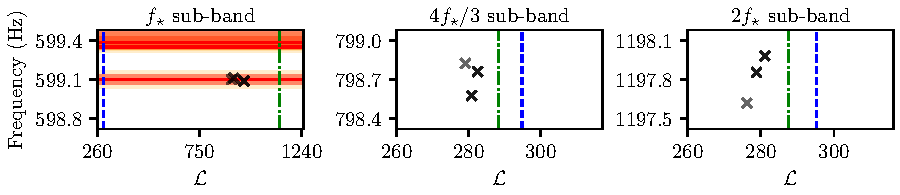
\includegraphics[width=\linewidth]{igr00291.pdf}
		\caption{Search results for \igra.}
		\label{fig:amxp_igra}	
	\end{subfigure}
	\par\vspace{2em} %
	\begin{subfigure}[t]{\textwidth}
		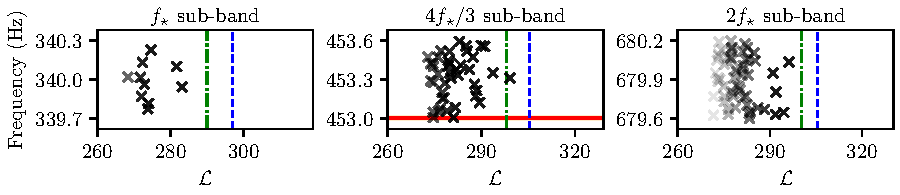
\includegraphics[width=\linewidth]{maxi0911.pdf}
		\caption{Search results for \maxi.}
		\label{fig:amxp_maxi}	
	\end{subfigure}
	\par\vspace{2em} %
	\begin{subfigure}[t]{\textwidth}
		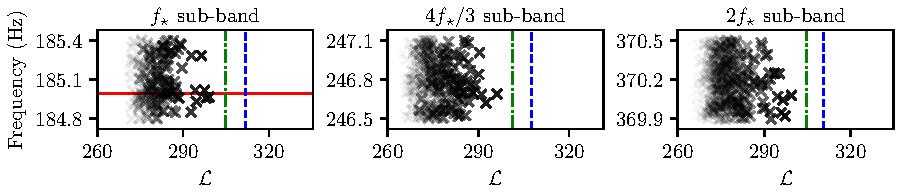
\includegraphics[width=\linewidth]{xte0929.pdf}
		\caption{Search results for \xtea.}
		\label{fig:amxp_xtea}	
	\end{subfigure}
	\par\vspace{2em} %	
	\begin{subfigure}[t]{\textwidth}
		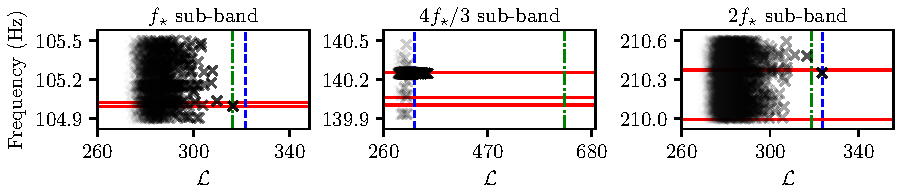
\includegraphics[width=\linewidth]{igr16597.pdf}
		\caption{Search results for \igrb.}
		\label{fig:amxp_igrb}	
	\end{subfigure}
	\par\vspace{2em} %
	\begin{subfigure}[t]{\textwidth}
		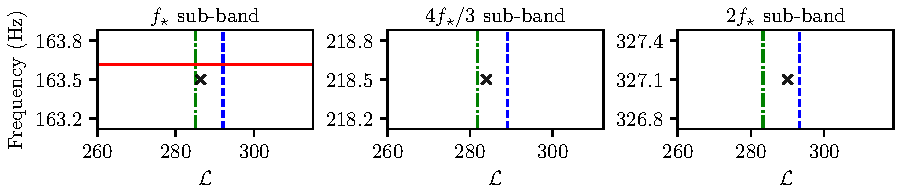
\includegraphics[width=\linewidth]{igr17062b.pdf}
		\caption{Search results for \igrc.}
		\label{fig:amxp_igrc}	
	\end{subfigure}
\end{figure*}
%
\begin{figure*}
	\ContinuedFloat
	\centering
	\begin{subfigure}[t]{\textwidth}
		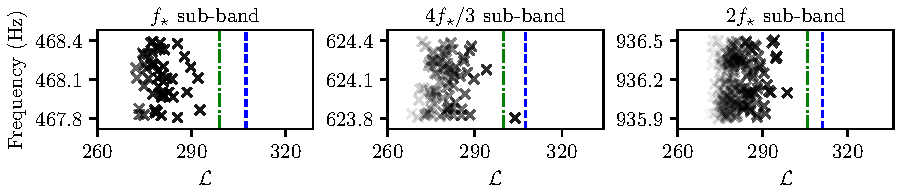
\includegraphics[width=\linewidth]{igr17379.pdf}
		\caption{Search results for \igrd.}
		\label{fig:amxp_igrd}	
	\end{subfigure}
	\par\vspace{2em} %
	\begin{subfigure}[t]{\textwidth}
		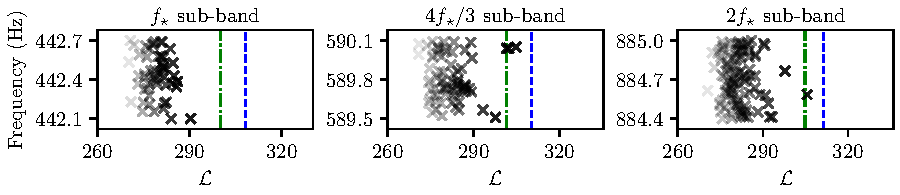
\includegraphics[width=\linewidth]{sax1748.pdf}
		\caption{Search results for \saxb.}
		\label{fig:amxp_saxb}	
	\end{subfigure}
	\par\vspace{2em} %
	\begin{subfigure}[t]{\textwidth}
		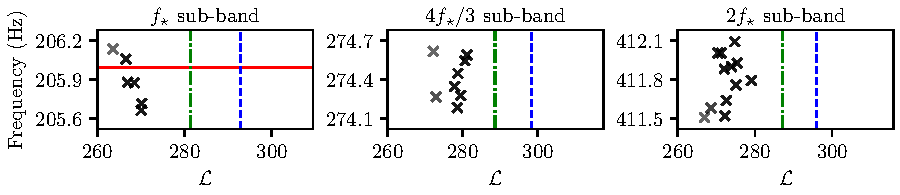
\includegraphics[width=\linewidth]{ngc6440x2.pdf}
		\caption{Search results for \ngc.}
		\label{fig:amxp_ngc}	
	\end{subfigure}
	\par\vspace{2em} %
	\begin{subfigure}[t]{\textwidth}
		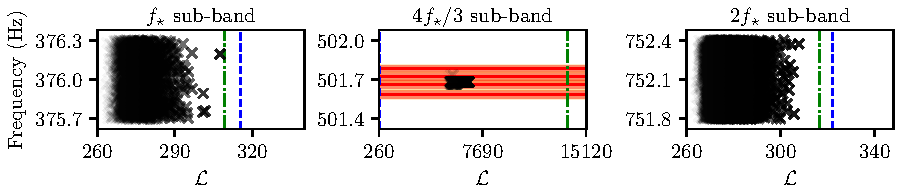
\includegraphics[width=\linewidth]{igr17494.pdf}
		\caption{Search results for \igri.}
		\label{fig:amxp_igri}	
	\end{subfigure}
	\par\vspace{2em} %
	\begin{subfigure}[t]{\textwidth}
		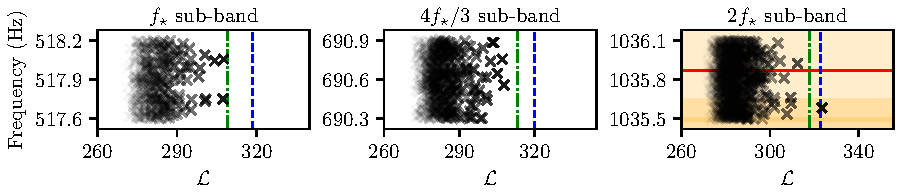
\includegraphics[width=\linewidth]{swift1749.pdf}
		\caption{Search results for \swiftb.}
		\label{fig:amxp_swiftb}	
	\end{subfigure}
\end{figure*}
%
\begin{figure*}
	\ContinuedFloat
	\centering
	\begin{subfigure}[t]{\textwidth}
		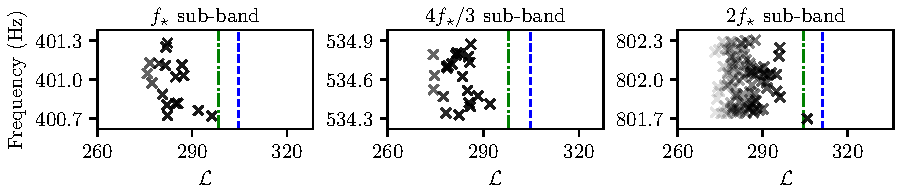
\includegraphics[width=\linewidth]{igr17498.pdf}
		\caption{Search results for \igre.}
		\label{fig:amxp_igre}	
	\end{subfigure}
	\par\vspace{2em} %
	\begin{subfigure}[t]{\textwidth}
		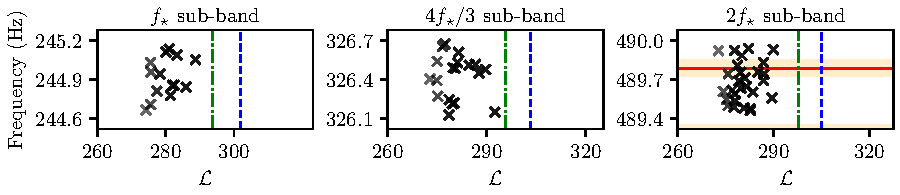
\includegraphics[width=\linewidth]{igr17511.pdf}
		\caption{Search results for \igrf.}
		\label{fig:amxp_igrf}	
	\end{subfigure}
	\par\vspace{2em} %
	\begin{subfigure}[t]{\textwidth}
		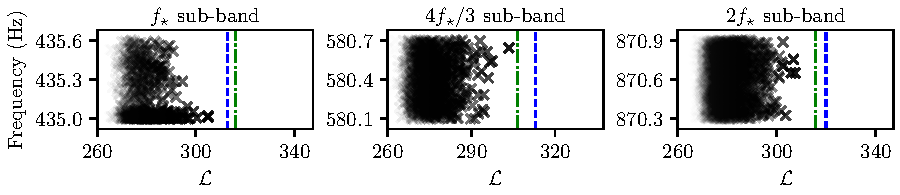
\includegraphics[width=\linewidth]{xte1751.pdf}
		\caption{Search results for \xteb.}
		\label{fig:amxp_xteb}	
	\end{subfigure}
	\par\vspace{2em} %
	\begin{subfigure}[t]{\textwidth}
		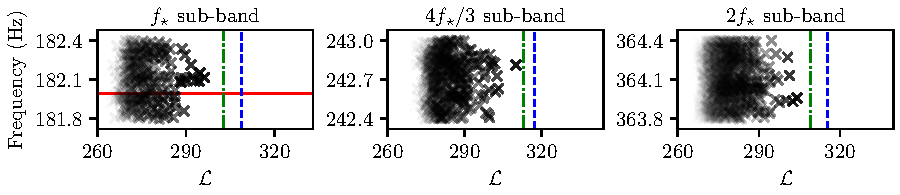
\includegraphics[width=\linewidth]{swift1756.pdf}
		\caption{Search results for \swift.}
		\label{fig:amxp_swift}	
	\end{subfigure}
	\par\vspace{2em} %
	\begin{subfigure}[t]{\textwidth}
		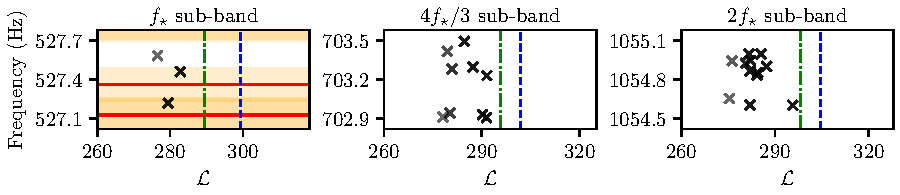
\includegraphics[width=\linewidth]{igr17591.pdf}
		\caption{Search results for \igrg.}
		\label{fig:amxp_igrg}	
	\end{subfigure}
\end{figure*}
%
\begin{figure*}
	\ContinuedFloat
	\centering			
	\begin{subfigure}[t]{\textwidth}
		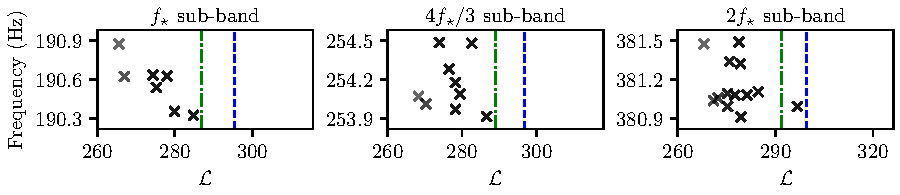
\includegraphics[width=\linewidth]{xte1807.pdf}
		\caption{Search results for \xtec.}
		\label{fig:amxp_xtec}	
	\end{subfigure}
	\par\vspace{2em} %
	\begin{subfigure}[t]{\textwidth}
		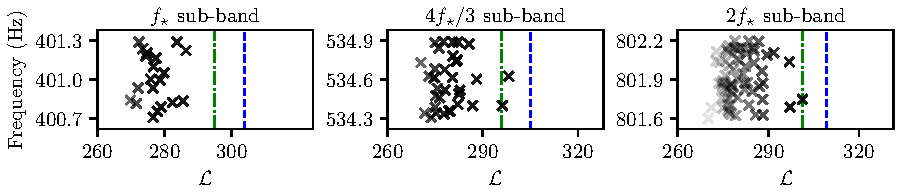
\includegraphics[width=\linewidth]{sax1808.pdf}
		\caption{Search results for \sax.}
		\label{fig:amxp_sax}	
	\end{subfigure}
	\par\vspace{2em} %
	\begin{subfigure}[t]{\textwidth}
		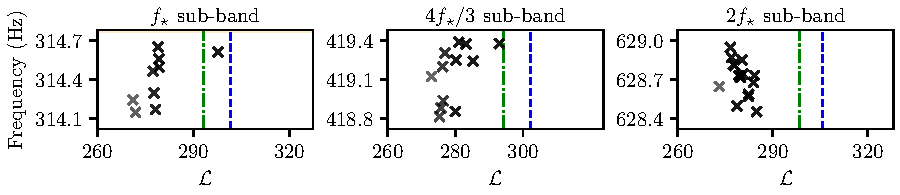
\includegraphics[width=\linewidth]{xte1814.pdf}
		\caption{Search results for \xted.}
		\label{fig:amxp_xted}	
	\end{subfigure}
	\par\vspace{2em} %
	\begin{subfigure}[t]{\textwidth}
		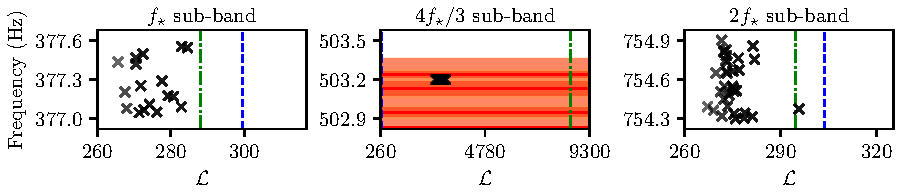
\includegraphics[width=\linewidth]{hete1900.pdf}
		\caption{Search results for \hete.}
		\label{fig:amxp_hete}	
	\end{subfigure}
	\par\vspace{2em} %
	\caption{Search results for each target and sub-band, laid out as in Fig \ref{fig:amxp_igrh}. Black crosses indicate the frequency and $\ml$ for the most likely path through the sub-band for each binary template. The vertical blue dashed (green dot-dashed) lines correspond to the threshold set via Gaussian (off-target) noise realizations, $\lthg$ ($\lthot$), in each sub-band. Solid red lines indicate the peak frequency of known instrumental lines in the detectors; the red band indicates the width of the line and the yellow band indicates the increased effective width due to Doppler broadening, as described in Sec.~\ref{sec:amxp_line_veto}. The transparency of crosses in sub-bands with many templates, e.g.~the sub-bands of \igrb, is adjusted relative to the maximum $\ml$ in that sub-band for clarity.}
\par\vspace{5em}
\label{fig:amxp_allfull}
\end{figure*}

\begin{figure*}
	\centering
	\begin{subfigure}[t]{0.49\textwidth}
		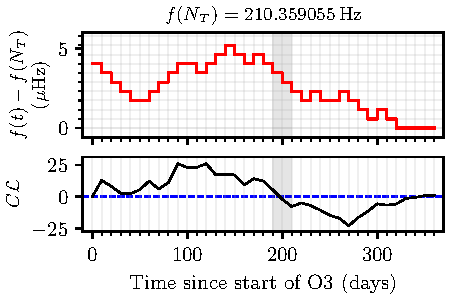
\includegraphics[width=\linewidth]{cumul_cpu_igr16597_210_1.pdf}
		\caption{\small Surviving candidate from \igrb.}
		\label{fig:amxp_igrb_f}	
	\end{subfigure}
	\hfill
	\begin{subfigure}[t]{0.49\textwidth}
		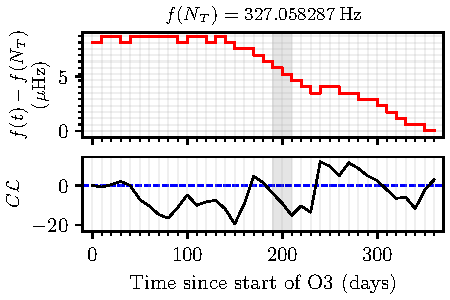
\includegraphics[width=\linewidth]{cumul_cpu_igr17062b_327_1.pdf}
		\caption{\small Surviving candidate from \igrc.}
		\label{fig:amxp_igrc_f}	
	\end{subfigure}
	\par\medskip %
	\begin{subfigure}[t]{0.49\textwidth}
		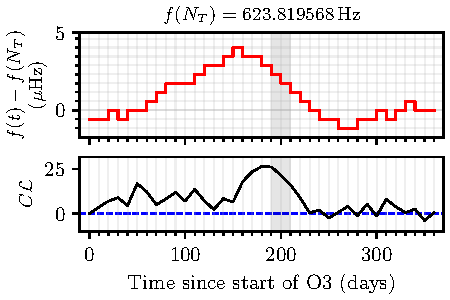
\includegraphics[width=\linewidth]{cumul_cpu_igr17379_624_1.pdf}
		\caption{\small Surviving candidate from \igrd.}
		\label{fig:amxp_igrd_f}	
	\end{subfigure}
	\hfill
	\begin{subfigure}[t]{0.49\textwidth}
		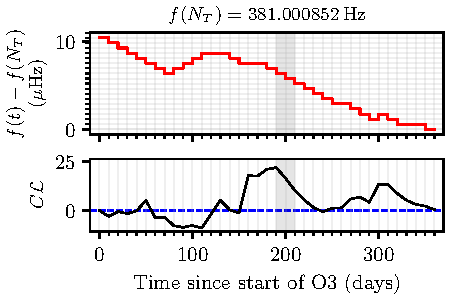
\includegraphics[width=\linewidth]{cumul_cpu_xte1807_381_1.pdf}
		\caption{\small Surviving candidate from \xtec.}
		\label{fig:amxp_xtec_f}
	\end{subfigure}
	\par\medskip %
	\begin{subfigure}[t]{0.49\textwidth}
		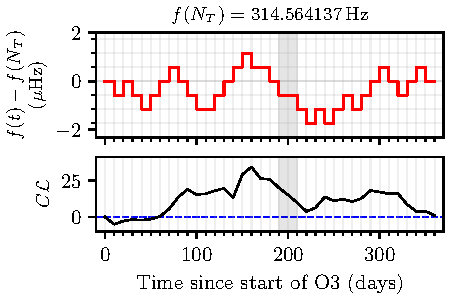
\includegraphics[width=\linewidth]{cumul_cpu_xte1814_314_1.pdf}
		\caption{\small Surviving candidate from \xted.}
		\label{fig:amxp_xted_f}
	\end{subfigure}
	\caption{Top panels: frequency paths, $f(t)$, for candidates with $\pn \leq 0.1$. The terminating frequency bin, $f(N_T)$, is subtracted and displayed in the title of each figure for clarity. Faint horizontal grey lines demarcate frequency bins of size $\Delta f = 5.787037\times10^{-7}\,$Hz, while faint vertical grey lines demarcate chunks of length $\tdr = 10\,$d. Bottom panels: the cumulative log-likelihood along the frequency path relative to the average sum log-likelihood needed to reach $\lth$, $C\ml \equiv \sum_{i=0}^{i=t}\big[\ml(i) - \lth / N_T\big]$, where $\sum_{i=0}^{i=t}\ml(i)$ is ${\rm ln\,} P(Q^*|O)$ from Eq.~\eqref{eq:amxp_probq_o} truncated after the $t$-th segment. The horizontal blue dashed line corresponds to $\sum_{i=0}^{i=t}\ml(i) = t \lth / N_T$. The grey shaded regions in both top and bottom panels correspond to the segments which have no SFTs and are therefore filled with a uniform log-likelihood, as described in Sec.~\ref{sec:amxp_o3data}.}
\label{fig:amxp_followups}
\end{figure*}
%

\begin{figure}
\centering
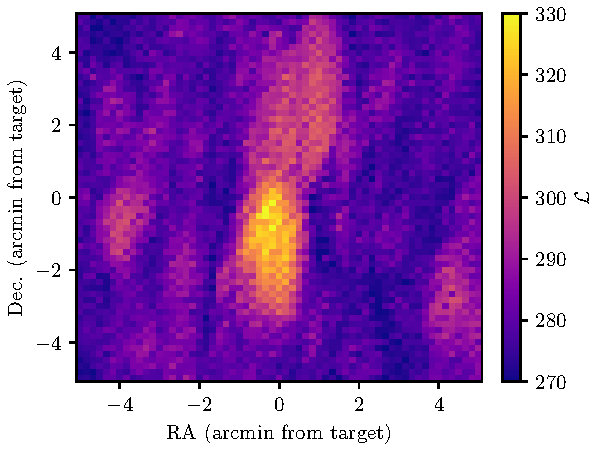
\includegraphics[width=0.8\linewidth]{igr16597_candidate-1_10-arcmin_3721-ntotal.pdf}
\caption{$\ml$, as represented by the color of each pixel, calculated at 3721 regularly spaced sky locations in a 100\,arcmin$^2$ patch of sky, centered on \igrb. See text in Appendix \ref{app:amxp_followup} for details.}
\label{fig:amxp_skymap}
\end{figure}

\newpage
\section{Survivor follow-up for target-of-opportunity search candidate \label{app:amxp_shortsax_followup}}
For posterity, and to aid future follow-up with different pipelines, we record in Table \ref{tab:shortsaxoutliers} the template, the frequency $f$, the log-likelihood $\ml$, and $\pn$, of the candidate from the target-of-opportunity search in Sec.~\ref{sec:amxp_shortsax} that survives all vetoes. 

As in Appendix \ref{app:amxp_followup}, we perform additional follow-up for this remaining candidate. With $T_{\rm obs}=24\,$d the point-spread-function of a moderately loud injection ($\ml \gtrsim \lth + 20$), at the sky location of the target, is a narrow ellipse $\sim2\,$arcmin wide in RA, but over $\sim30\,$arcmin tall in Dec. When we search a 100\,arcmin$^2$ patch of sky around the location of \sax\ we do not see any evidence of this point-spread-function at the source location. There is an ellipse with $\ml > \lth$ roughly $-2\,$arcmin away in RA from \sax, but as the location of the target is known to sub-arcsec precision \cite{Bult2020}, this ellipse is likely a noise fluctuation, rather than an astrophysical signal.

We also calculate $\ml$ in a small, densely sampled patch of the $\{P,\ \tasc\}$ parameter space around the candidate's template. As discussed in Appendix \ref{app:amxp_followup}, moderately loud injections ($\ml \gtrsim \lth + 20$) ``spread out'' in the $\{P,\ \tasc\}$ plane. However, the candidate is not loud enough for this diagnostic to provide evidence for or against the hypothesis that the candidate is a noise fluctuation.

\begin{table*}
	\centering
	\caption{Orbital template, $(P,\ a_0,\ \tasc)$, frequency, $f$, log-likelihood, $\ml$, and the probability of seeing a candidate at least this loud in pure noise, $\pn$, for the remaining candidate from the target-of-opportunity, $24\,$d coherent search when \sax\ was in outburst. The candidate cannot be eliminated by any of the vetoes detailed in Sec.~\ref{sec:amxp_vetoes}. \label{tab:shortsaxoutliers}}
	\begin{tabular}{r r r r r r}
	\toprule
		\textrm{$P$ (s)} & \textrm{$a_0$ (lt-s)} & \textrm{$\tasc$ (GPS time)} & \textrm{$f$ (Hz)} & \textrm{$\ml$} & \textrm{$\pn$} \\
	\midrule
	7249.155 & 0.062809 & 1249163578.03125 & 400.59656098 & 42.5 & 0.02 \\
	\bottomrule
	\end{tabular}
\end{table*}
	
If we assume that the remaining candidate is a false alarm, we calculate $\hul$ for the $24\,$d coherent search, using the procedure outlined in Sec.~\ref{sec:amxp_ul_method}. We find $\hul = 1.3\times 10^{-25}$ for the sub-bands centered on $f_\star$ and $4f_\star/3$, and $\hul = 1.7\times 10^{-25}$ for the sub-band centered on $2f_\star$. These upper limits are higher than the ones listed in Sec.~\ref{sec:amxp_ul_results} because the longer coherence time does not completely compensate for the shorter observation time.

Finally, we perform a complementary follow-up search using a deterministic signal template on the candidate of interest using \texttt{PyFstat} \cite{Ashton:2018ure, Keitel:2021xeq}. The use of the \texttt{PyFstat} algorithm as a follow-up technique was applied to the last surviving outlier of \citet{o3aAllSkyIso} and previously in \citet{Covas:2020nwy, o3abinaryallsky}.
The follow-up procedure, thoroughly described in \citet{Tenorio:2021njf}, uses a Markov chain Monte Carlo (MCMC) sampler \cite{emcee, ptemcee} to explore a parameter-space region using the $\mathcal{F}$-statistic 
as log-likelihood \cite{JKS98}. Two coherence times are used here, namely $T_{\textrm{coh}} = 12\,\textrm{d}$ and $T_{\textrm{coh}} = 24\,\textrm{d}$. Prior distributions 
are Gaussian distributions centered at the outlier parameters (Table~\ref{tab:shortsaxoutliers}) using a standard deviation of one parameter-space bin with maximum mismatch $\mu_{\textrm{max}}=1$ \cite{Leaci2015}. 
The results of the follow-up are evaluated using a Bayes factor, $\mathcal{B}_{\textrm{S}/\textrm{N}}$, that compares the evidence for a model that the data contain a coherent signal to the 
evidence for a model that the data contain only noise.
The value of $\mathcal{B}_{\textrm{S}/\textrm{N}}$ is computed by comparing the change in the $\mathcal{F}$-statistic of the 
loudest candidate between the two follow-up stages with different coherence times: if a signal is present in the data, the $\mathcal{F}$-statistic should provide a consistent estimate of the  
signal-to-noise ratio; otherwise, the loudest candidate is a result of noise, the distribution of which follows a Gumbel distribution. This noise distribution is estimated using a similar method to the one described in Appendix~\ref{app:amxp_offt_th}, with 600 off-source calculations performed. 

The loudest candidate of the follow-up returns a log-Bayes factor of 
$\log_{10}\mathcal{B}_{\textrm{S}/\textrm{N}} = 1.45$. We characterize the 
$\log_{10}\mathcal{B}_{\textrm{S}/\textrm{N}}$ distribution using 400 isotropically distributed sources
injected into the real data with an amplitude of $\hul$. We obtain a 1\% false dismissal threshold of 8.75, 
which is significantly larger than the candidate's log-Bayes factor of 1.45. That is, if this were a true signal, 
with $h_0 = \hul$, we would expect the log-Bayes factor to be higher than what we see in the real data by about 7.
We conclude that there is no significant evidence of continuous gravitational wave emission from this target.

% \section{Full author list} \label{app:amxp_authors}

% \author{R.~Abbott}
\affiliation{LIGO Laboratory, California Institute of Technology, Pasadena, CA 91125, USA}
\author{T.~D.~Abbott}
\affiliation{Louisiana State University, Baton Rouge, LA 70803, USA}
\author{F.~Acernese}
\affiliation{Dipartimento di Farmacia, Universit\`a di Salerno, I-84084 Fisciano, Salerno, Italy}
\affiliation{INFN, Sezione di Napoli, Complesso Universitario di Monte S. Angelo, I-80126 Napoli, Italy}
\author{K.~Ackley}
\affiliation{OzGrav, School of Physics \& Astronomy, Monash University, Clayton 3800, Victoria, Australia}
\author{C.~Adams}
\affiliation{LIGO Livingston Observatory, Livingston, LA 70754, USA}
\author{N.~Adhikari}
\affiliation{University of Wisconsin-Milwaukee, Milwaukee, WI 53201, USA}
\author{R.~X.~Adhikari}
\affiliation{LIGO Laboratory, California Institute of Technology, Pasadena, CA 91125, USA}
\author{V.~B.~Adya}
\affiliation{OzGrav, Australian National University, Canberra, Australian Capital Territory 0200, Australia}
\author{C.~Affeldt}
\affiliation{Max Planck Institute for Gravitational Physics (Albert Einstein Institute), D-30167 Hannover, Germany}
\affiliation{Leibniz Universit\"at Hannover, D-30167 Hannover, Germany}
\author{D.~Agarwal}
\affiliation{Inter-University Centre for Astronomy and Astrophysics, Pune 411007, India}
\author{M.~Agathos}
\affiliation{University of Cambridge, Cambridge CB2 1TN, United Kingdom}
\affiliation{Theoretisch-Physikalisches Institut, Friedrich-Schiller-Universit\"at Jena, D-07743 Jena, Germany}
\author{K.~Agatsuma}
\affiliation{University of Birmingham, Birmingham B15 2TT, United Kingdom}
\author{N.~Aggarwal}
\affiliation{Center for Interdisciplinary Exploration \& Research in Astrophysics (CIERA), Northwestern University, Evanston, IL 60208, USA}
\author{O.~D.~Aguiar}
\affiliation{Instituto Nacional de Pesquisas Espaciais, 12227-010 S\~{a}o Jos\'{e} dos Campos, S\~{a}o Paulo, Brazil}
\author{L.~Aiello}
\affiliation{Gravity Exploration Institute, Cardiff University, Cardiff CF24 3AA, United Kingdom}
\author{A.~Ain}
\affiliation{INFN, Sezione di Pisa, I-56127 Pisa, Italy}
\author{T.~Akutsu}
\affiliation{Gravitational Wave Science Project, National Astronomical Observatory of Japan (NAOJ), Mitaka City, Tokyo 181-8588, Japan}
\affiliation{Advanced Technology Center, National Astronomical Observatory of Japan (NAOJ), Mitaka City, Tokyo 181-8588, Japan}
\author{S.~Albanesi}
\affiliation{INFN Sezione di Torino, I-10125 Torino, Italy}
\author{A.~Allocca}
\affiliation{Universit\`a di Napoli ``Federico II'', Complesso Universitario di Monte S. Angelo, I-80126 Napoli, Italy}
\affiliation{INFN, Sezione di Napoli, Complesso Universitario di Monte S. Angelo, I-80126 Napoli, Italy}
\author{P.~A.~Altin}
\affiliation{OzGrav, Australian National University, Canberra, Australian Capital Territory 0200, Australia}
\author{A.~Amato}
\affiliation{Universit\'e de Lyon, Universit\'e Claude Bernard Lyon 1, CNRS, Institut Lumi\`ere Mati\`ere, F-69622 Villeurbanne, France}
\author{C.~Anand}
\affiliation{OzGrav, School of Physics \& Astronomy, Monash University, Clayton 3800, Victoria, Australia}
\author{S.~Anand}
\affiliation{LIGO Laboratory, California Institute of Technology, Pasadena, CA 91125, USA}
\author{A.~Ananyeva}
\affiliation{LIGO Laboratory, California Institute of Technology, Pasadena, CA 91125, USA}
\author{S.~B.~Anderson}
\affiliation{LIGO Laboratory, California Institute of Technology, Pasadena, CA 91125, USA}
\author{W.~G.~Anderson}
\affiliation{University of Wisconsin-Milwaukee, Milwaukee, WI 53201, USA}
\author{M.~Ando}
\affiliation{Department of Physics, The University of Tokyo, Bunkyo-ku, Tokyo 113-0033, Japan}
\affiliation{Research Center for the Early Universe (RESCEU), The University of Tokyo, Bunkyo-ku, Tokyo 113-0033, Japan}
\author{T.~Andrade}
\affiliation{Institut de Ci\`encies del Cosmos (ICCUB), Universitat de Barcelona, C/ Mart\'i i Franqu\`es 1, Barcelona, 08028, Spain}
\author{N.~Andres}
\affiliation{Laboratoire d'Annecy de Physique des Particules (LAPP), Univ. Grenoble Alpes, Universit\'e Savoie Mont Blanc, CNRS/IN2P3, F-74941 Annecy, France}
\author{T.~Andri\'c}
\affiliation{Gran Sasso Science Institute (GSSI), I-67100 L'Aquila, Italy}
\author{S.~V.~Angelova}
\affiliation{SUPA, University of Strathclyde, Glasgow G1 1XQ, United Kingdom}
\author{S.~Ansoldi}
\affiliation{Dipartimento di Scienze Matematiche, Informatiche e Fisiche, Universit\`a di Udine, I-33100 Udine, Italy}
\affiliation{INFN, Sezione di Trieste, I-34127 Trieste, Italy}
\author{J.~M.~Antelis}
\affiliation{Embry-Riddle Aeronautical University, Prescott, AZ 86301, USA}
\author{S.~Antier}
\affiliation{Universit\'e de Paris, CNRS, Astroparticule et Cosmologie, F-75006 Paris, France}
\author{S.~Appert}
\affiliation{LIGO Laboratory, California Institute of Technology, Pasadena, CA 91125, USA}
\author{Koji~Arai}
\affiliation{LIGO Laboratory, California Institute of Technology, Pasadena, CA 91125, USA}
\author{Koya~Arai}
\affiliation{Institute for Cosmic Ray Research (ICRR), KAGRA Observatory, The University of Tokyo, Kashiwa City, Chiba 277-8582, Japan}
\author{Y.~Arai}
\affiliation{Institute for Cosmic Ray Research (ICRR), KAGRA Observatory, The University of Tokyo, Kashiwa City, Chiba 277-8582, Japan}
\author{S.~Araki}
\affiliation{Accelerator Laboratory, High Energy Accelerator Research Organization (KEK), Tsukuba City, Ibaraki 305-0801, Japan}
\author{A.~Araya}
\affiliation{Earthquake Research Institute, The University of Tokyo, Bunkyo-ku, Tokyo 113-0032, Japan}
\author{M.~C.~Araya}
\affiliation{LIGO Laboratory, California Institute of Technology, Pasadena, CA 91125, USA}
\author{J.~S.~Areeda}
\affiliation{California State University Fullerton, Fullerton, CA 92831, USA}
\author{M.~Ar\`ene}
\affiliation{Universit\'e de Paris, CNRS, Astroparticule et Cosmologie, F-75006 Paris, France}
\author{N.~Aritomi}
\affiliation{Department of Physics, The University of Tokyo, Bunkyo-ku, Tokyo 113-0033, Japan}
\author{N.~Arnaud}
\affiliation{Universit\'e Paris-Saclay, CNRS/IN2P3, IJCLab, 91405 Orsay, France}
\affiliation{European Gravitational Observatory (EGO), I-56021 Cascina, Pisa, Italy}
\author{S.~M.~Aronson}
\affiliation{Louisiana State University, Baton Rouge, LA 70803, USA}
\author{K.~G.~Arun}
\affiliation{Chennai Mathematical Institute, Chennai 603103, India}
\author{H.~Asada}
\affiliation{Department of Mathematics and Physics, Gravitational Wave Science Project, Hirosaki University, Hirosaki City, Aomori 036-8561, Japan}
\author{Y.~Asali}
\affiliation{Columbia University, New York, NY 10027, USA}
\author{G.~Ashton}
\affiliation{OzGrav, School of Physics \& Astronomy, Monash University, Clayton 3800, Victoria, Australia}
\author{Y.~Aso}
\affiliation{Kamioka Branch, National Astronomical Observatory of Japan (NAOJ), Kamioka-cho, Hida City, Gifu 506-1205, Japan}
\affiliation{The Graduate University for Advanced Studies (SOKENDAI), Mitaka City, Tokyo 181-8588, Japan}
\author{M.~Assiduo}
\affiliation{Universit\`a degli Studi di Urbino ``Carlo Bo'', I-61029 Urbino, Italy}
\affiliation{INFN, Sezione di Firenze, I-50019 Sesto Fiorentino, Firenze, Italy}
\author{S.~M.~Aston}
\affiliation{LIGO Livingston Observatory, Livingston, LA 70754, USA}
\author{P.~Astone}
\affiliation{INFN, Sezione di Roma, I-00185 Roma, Italy}
\author{F.~Aubin}
\affiliation{Laboratoire d'Annecy de Physique des Particules (LAPP), Univ. Grenoble Alpes, Universit\'e Savoie Mont Blanc, CNRS/IN2P3, F-74941 Annecy, France}
\author{C.~Austin}
\affiliation{Louisiana State University, Baton Rouge, LA 70803, USA}
\author{S.~Babak}
\affiliation{Universit\'e de Paris, CNRS, Astroparticule et Cosmologie, F-75006 Paris, France}
\author{F.~Badaracco}
\affiliation{Universit\'e catholique de Louvain, B-1348 Louvain-la-Neuve, Belgium}
\author{M.~K.~M.~Bader}
\affiliation{Nikhef, Science Park 105, 1098 XG Amsterdam, Netherlands}
\author{C.~Badger}
\affiliation{King's College London, University of London, London WC2R 2LS, United Kingdom}
\author{S.~Bae}
\affiliation{Korea Institute of Science and Technology Information (KISTI), Yuseong-gu, Daejeon 34141, Korea}
\author{Y.~Bae}
\affiliation{National Institute for Mathematical Sciences, Yuseong-gu, Daejeon 34047, Korea}
\author{A.~M.~Baer}
\affiliation{Christopher Newport University, Newport News, VA 23606, USA}
\author{S.~Bagnasco}
\affiliation{INFN Sezione di Torino, I-10125 Torino, Italy}
\author{Y.~Bai}
\affiliation{LIGO Laboratory, California Institute of Technology, Pasadena, CA 91125, USA}
\author{L.~Baiotti}
\affiliation{International College, Osaka University, Toyonaka City, Osaka 560-0043, Japan}
\author{J.~Baird}
\affiliation{Universit\'e de Paris, CNRS, Astroparticule et Cosmologie, F-75006 Paris, France}
\author{R.~Bajpai}
\affiliation{School of High Energy Accelerator Science, The Graduate University for Advanced Studies (SOKENDAI), Tsukuba City, Ibaraki 305-0801, Japan}
\author{M.~Ball}
\affiliation{University of Oregon, Eugene, OR 97403, USA}
\author{G.~Ballardin}
\affiliation{European Gravitational Observatory (EGO), I-56021 Cascina, Pisa, Italy}
\author{S.~W.~Ballmer}
\affiliation{Syracuse University, Syracuse, NY 13244, USA}
\author{A.~Balsamo}
\affiliation{Christopher Newport University, Newport News, VA 23606, USA}
\author{G.~Baltus}
\affiliation{Universit\'e de Li\`ege, B-4000 Li\`ege, Belgium}
\author{S.~Banagiri}
\affiliation{University of Minnesota, Minneapolis, MN 55455, USA}
\author{D.~Bankar}
\affiliation{Inter-University Centre for Astronomy and Astrophysics, Pune 411007, India}
\author{J.~C.~Barayoga}
\affiliation{LIGO Laboratory, California Institute of Technology, Pasadena, CA 91125, USA}
\author{C.~Barbieri}
\affiliation{Universit\`a degli Studi di Milano-Bicocca, I-20126 Milano, Italy}
\affiliation{INFN, Sezione di Milano-Bicocca, I-20126 Milano, Italy}
\affiliation{INAF, Osservatorio Astronomico di Brera sede di Merate, I-23807 Merate, Lecco, Italy}
\author{B.~C.~Barish}
\affiliation{LIGO Laboratory, California Institute of Technology, Pasadena, CA 91125, USA}
\author{D.~Barker}
\affiliation{LIGO Hanford Observatory, Richland, WA 99352, USA}
\author{P.~Barneo}
\affiliation{Institut de Ci\`encies del Cosmos (ICCUB), Universitat de Barcelona, C/ Mart\'i i Franqu\`es 1, Barcelona, 08028, Spain}
\author{F.~Barone}
\affiliation{Dipartimento di Medicina, Chirurgia e Odontoiatria ``Scuola Medica Salernitana'', Universit\`a di Salerno, I-84081 Baronissi, Salerno, Italy}
\affiliation{INFN, Sezione di Napoli, Complesso Universitario di Monte S. Angelo, I-80126 Napoli, Italy}
\author{B.~Barr}
\affiliation{SUPA, University of Glasgow, Glasgow G12 8QQ, United Kingdom}
\author{L.~Barsotti}
\affiliation{LIGO Laboratory, Massachusetts Institute of Technology, Cambridge, MA 02139, USA}
\author{M.~Barsuglia}
\affiliation{Universit\'e de Paris, CNRS, Astroparticule et Cosmologie, F-75006 Paris, France}
\author{D.~Barta}
\affiliation{Wigner RCP, RMKI, H-1121 Budapest, Konkoly Thege Mikl\'os \'ut 29-33, Hungary}
\author{J.~Bartlett}
\affiliation{LIGO Hanford Observatory, Richland, WA 99352, USA}
\author{M.~A.~Barton}
\affiliation{SUPA, University of Glasgow, Glasgow G12 8QQ, United Kingdom}
\affiliation{Gravitational Wave Science Project, National Astronomical Observatory of Japan (NAOJ), Mitaka City, Tokyo 181-8588, Japan}
\author{I.~Bartos}
\affiliation{University of Florida, Gainesville, FL 32611, USA}
\author{R.~Bassiri}
\affiliation{Stanford University, Stanford, CA 94305, USA}
\author{A.~Basti}
\affiliation{Universit\`a di Pisa, I-56127 Pisa, Italy}
\affiliation{INFN, Sezione di Pisa, I-56127 Pisa, Italy}
\author{M.~Bawaj}
\affiliation{INFN, Sezione di Perugia, I-06123 Perugia, Italy}
\affiliation{Universit\`a di Perugia, I-06123 Perugia, Italy}
\author{J.~C.~Bayley}
\affiliation{SUPA, University of Glasgow, Glasgow G12 8QQ, United Kingdom}
\author{A.~C.~Baylor}
\affiliation{University of Wisconsin-Milwaukee, Milwaukee, WI 53201, USA}
\author{M.~Bazzan}
\affiliation{Universit\`a di Padova, Dipartimento di Fisica e Astronomia, I-35131 Padova, Italy}
\affiliation{INFN, Sezione di Padova, I-35131 Padova, Italy}
\author{B.~B\'ecsy}
\affiliation{Montana State University, Bozeman, MT 59717, USA}
\author{V.~M.~Bedakihale}
\affiliation{Institute for Plasma Research, Bhat, Gandhinagar 382428, India}
\author{M.~Bejger}
\affiliation{Nicolaus Copernicus Astronomical Center, Polish Academy of Sciences, 00-716, Warsaw, Poland}
\author{I.~Belahcene}
\affiliation{Universit\'e Paris-Saclay, CNRS/IN2P3, IJCLab, 91405 Orsay, France}
\author{V.~Benedetto}
\affiliation{Dipartimento di Ingegneria, Universit\`a del Sannio, I-82100 Benevento, Italy}
\author{D.~Beniwal}
\affiliation{OzGrav, University of Adelaide, Adelaide, South Australia 5005, Australia}
\author{T.~F.~Bennett}
\affiliation{California State University, Los Angeles, 5151 State University Dr, Los Angeles, CA 90032, USA}
\author{J.~D.~Bentley}
\affiliation{University of Birmingham, Birmingham B15 2TT, United Kingdom}
\author{M.~BenYaala}
\affiliation{SUPA, University of Strathclyde, Glasgow G1 1XQ, United Kingdom}
\author{F.~Bergamin}
\affiliation{Max Planck Institute for Gravitational Physics (Albert Einstein Institute), D-30167 Hannover, Germany}
\affiliation{Leibniz Universit\"at Hannover, D-30167 Hannover, Germany}
\author{B.~K.~Berger}
\affiliation{Stanford University, Stanford, CA 94305, USA}
\author{S.~Bernuzzi}
\affiliation{Theoretisch-Physikalisches Institut, Friedrich-Schiller-Universit\"at Jena, D-07743 Jena, Germany}
\author{D.~Bersanetti}
\affiliation{INFN, Sezione di Genova, I-16146 Genova, Italy}
\author{A.~Bertolini}
\affiliation{Nikhef, Science Park 105, 1098 XG Amsterdam, Netherlands}
\author{J.~Betzwieser}
\affiliation{LIGO Livingston Observatory, Livingston, LA 70754, USA}
\author{D.~Beveridge}
\affiliation{OzGrav, University of Western Australia, Crawley, Western Australia 6009, Australia}
\author{R.~Bhandare}
\affiliation{RRCAT, Indore, Madhya Pradesh 452013, India}
\author{U.~Bhardwaj}
\affiliation{GRAPPA, Anton Pannekoek Institute for Astronomy and Institute for High-Energy Physics, University of Amsterdam, Science Park 904, 1098 XH Amsterdam, Netherlands}
\affiliation{Nikhef, Science Park 105, 1098 XG Amsterdam, Netherlands}
\author{D.~Bhattacharjee}
\affiliation{Missouri University of Science and Technology, Rolla, MO 65409, USA}
\author{S.~Bhaumik}
\affiliation{University of Florida, Gainesville, FL 32611, USA}
\author{I.~A.~Bilenko}
\affiliation{Faculty of Physics, Lomonosov Moscow State University, Moscow 119991, Russia}
\author{G.~Billingsley}
\affiliation{LIGO Laboratory, California Institute of Technology, Pasadena, CA 91125, USA}
\author{S.~Bini}
\affiliation{Universit\`a di Trento, Dipartimento di Fisica, I-38123 Povo, Trento, Italy}
\affiliation{INFN, Trento Institute for Fundamental Physics and Applications, I-38123 Povo, Trento, Italy}
\author{R.~Birney}
\affiliation{SUPA, University of the West of Scotland, Paisley PA1 2BE, United Kingdom}
\author{O.~Birnholtz}
\affiliation{Bar-Ilan University, Ramat Gan, 5290002, Israel}
\author{S.~Biscans}
\affiliation{LIGO Laboratory, California Institute of Technology, Pasadena, CA 91125, USA}
\affiliation{LIGO Laboratory, Massachusetts Institute of Technology, Cambridge, MA 02139, USA}
\author{M.~Bischi}
\affiliation{Universit\`a degli Studi di Urbino ``Carlo Bo'', I-61029 Urbino, Italy}
\affiliation{INFN, Sezione di Firenze, I-50019 Sesto Fiorentino, Firenze, Italy}
\author{S.~Biscoveanu}
\affiliation{LIGO Laboratory, Massachusetts Institute of Technology, Cambridge, MA 02139, USA}
\author{A.~Bisht}
\affiliation{Max Planck Institute for Gravitational Physics (Albert Einstein Institute), D-30167 Hannover, Germany}
\affiliation{Leibniz Universit\"at Hannover, D-30167 Hannover, Germany}
\author{B.~Biswas}
\affiliation{Inter-University Centre for Astronomy and Astrophysics, Pune 411007, India}
\author{M.~Bitossi}
\affiliation{European Gravitational Observatory (EGO), I-56021 Cascina, Pisa, Italy}
\affiliation{INFN, Sezione di Pisa, I-56127 Pisa, Italy}
\author{M.-A.~Bizouard}
\affiliation{Artemis, Universit\'e C\^ote d'Azur, Observatoire de la C\^ote d'Azur, CNRS, F-06304 Nice, France}
\author{J.~K.~Blackburn}
\affiliation{LIGO Laboratory, California Institute of Technology, Pasadena, CA 91125, USA}
\author{C.~D.~Blair}
\affiliation{OzGrav, University of Western Australia, Crawley, Western Australia 6009, Australia}
\affiliation{LIGO Livingston Observatory, Livingston, LA 70754, USA}
\author{D.~G.~Blair}
\affiliation{OzGrav, University of Western Australia, Crawley, Western Australia 6009, Australia}
\author{R.~M.~Blair}
\affiliation{LIGO Hanford Observatory, Richland, WA 99352, USA}
\author{F.~Bobba}
\affiliation{Dipartimento di Fisica ``E.R. Caianiello'', Universit\`a di Salerno, I-84084 Fisciano, Salerno, Italy}
\affiliation{INFN, Sezione di Napoli, Gruppo Collegato di Salerno, Complesso Universitario di Monte S. Angelo, I-80126 Napoli, Italy}
\author{N.~Bode}
\affiliation{Max Planck Institute for Gravitational Physics (Albert Einstein Institute), D-30167 Hannover, Germany}
\affiliation{Leibniz Universit\"at Hannover, D-30167 Hannover, Germany}
\author{M.~Boer}
\affiliation{Artemis, Universit\'e C\^ote d'Azur, Observatoire de la C\^ote d'Azur, CNRS, F-06304 Nice, France}
\author{G.~Bogaert}
\affiliation{Artemis, Universit\'e C\^ote d'Azur, Observatoire de la C\^ote d'Azur, CNRS, F-06304 Nice, France}
\author{M.~Boldrini}
\affiliation{Universit\`a di Roma ``La Sapienza'', I-00185 Roma, Italy}
\affiliation{INFN, Sezione di Roma, I-00185 Roma, Italy}
\author{L.~D.~Bonavena}
\affiliation{Universit\`a di Padova, Dipartimento di Fisica e Astronomia, I-35131 Padova, Italy}
\author{F.~Bondu}
\affiliation{Univ Rennes, CNRS, Institut FOTON - UMR6082, F-3500 Rennes, France}
\author{E.~Bonilla}
\affiliation{Stanford University, Stanford, CA 94305, USA}
\author{R.~Bonnand}
\affiliation{Laboratoire d'Annecy de Physique des Particules (LAPP), Univ. Grenoble Alpes, Universit\'e Savoie Mont Blanc, CNRS/IN2P3, F-74941 Annecy, France}
\author{P.~Booker}
\affiliation{Max Planck Institute for Gravitational Physics (Albert Einstein Institute), D-30167 Hannover, Germany}
\affiliation{Leibniz Universit\"at Hannover, D-30167 Hannover, Germany}
\author{B.~A.~Boom}
\affiliation{Nikhef, Science Park 105, 1098 XG Amsterdam, Netherlands}
\author{R.~Bork}
\affiliation{LIGO Laboratory, California Institute of Technology, Pasadena, CA 91125, USA}
\author{V.~Boschi}
\affiliation{INFN, Sezione di Pisa, I-56127 Pisa, Italy}
\author{N.~Bose}
\affiliation{Indian Institute of Technology Bombay, Powai, Mumbai 400 076, India}
\author{S.~Bose}
\affiliation{Inter-University Centre for Astronomy and Astrophysics, Pune 411007, India}
\author{V.~Bossilkov}
\affiliation{OzGrav, University of Western Australia, Crawley, Western Australia 6009, Australia}
\author{V.~Boudart}
\affiliation{Universit\'e de Li\`ege, B-4000 Li\`ege, Belgium}
\author{Y.~Bouffanais}
\affiliation{Universit\`a di Padova, Dipartimento di Fisica e Astronomia, I-35131 Padova, Italy}
\affiliation{INFN, Sezione di Padova, I-35131 Padova, Italy}
\author{A.~Bozzi}
\affiliation{European Gravitational Observatory (EGO), I-56021 Cascina, Pisa, Italy}
\author{C.~Bradaschia}
\affiliation{INFN, Sezione di Pisa, I-56127 Pisa, Italy}
\author{P.~R.~Brady}
\affiliation{University of Wisconsin-Milwaukee, Milwaukee, WI 53201, USA}
\author{A.~Bramley}
\affiliation{LIGO Livingston Observatory, Livingston, LA 70754, USA}
\author{A.~Branch}
\affiliation{LIGO Livingston Observatory, Livingston, LA 70754, USA}
\author{M.~Branchesi}
\affiliation{Gran Sasso Science Institute (GSSI), I-67100 L'Aquila, Italy}
\affiliation{INFN, Laboratori Nazionali del Gran Sasso, I-67100 Assergi, Italy}
\author{J.~E.~Brau}
\affiliation{University of Oregon, Eugene, OR 97403, USA}
\author{M.~Breschi}
\affiliation{Theoretisch-Physikalisches Institut, Friedrich-Schiller-Universit\"at Jena, D-07743 Jena, Germany}
\author{T.~Briant}
\affiliation{Laboratoire Kastler Brossel, Sorbonne Universit\'e, CNRS, ENS-Universit\'e PSL, Coll\`ege de France, F-75005 Paris, France}
\author{J.~H.~Briggs}
\affiliation{SUPA, University of Glasgow, Glasgow G12 8QQ, United Kingdom}
\author{A.~Brillet}
\affiliation{Artemis, Universit\'e C\^ote d'Azur, Observatoire de la C\^ote d'Azur, CNRS, F-06304 Nice, France}
\author{M.~Brinkmann}
\affiliation{Max Planck Institute for Gravitational Physics (Albert Einstein Institute), D-30167 Hannover, Germany}
\affiliation{Leibniz Universit\"at Hannover, D-30167 Hannover, Germany}
\author{P.~Brockill}
\affiliation{University of Wisconsin-Milwaukee, Milwaukee, WI 53201, USA}
\author{A.~F.~Brooks}
\affiliation{LIGO Laboratory, California Institute of Technology, Pasadena, CA 91125, USA}
\author{J.~Brooks}
\affiliation{European Gravitational Observatory (EGO), I-56021 Cascina, Pisa, Italy}
\author{D.~D.~Brown}
\affiliation{OzGrav, University of Adelaide, Adelaide, South Australia 5005, Australia}
\author{S.~Brunett}
\affiliation{LIGO Laboratory, California Institute of Technology, Pasadena, CA 91125, USA}
\author{G.~Bruno}
\affiliation{Universit\'e catholique de Louvain, B-1348 Louvain-la-Neuve, Belgium}
\author{R.~Bruntz}
\affiliation{Christopher Newport University, Newport News, VA 23606, USA}
\author{J.~Bryant}
\affiliation{University of Birmingham, Birmingham B15 2TT, United Kingdom}
\author{T.~Bulik}
\affiliation{Astronomical Observatory Warsaw University, 00-478 Warsaw, Poland}
\author{H.~J.~Bulten}
\affiliation{Nikhef, Science Park 105, 1098 XG Amsterdam, Netherlands}
\author{A.~Buonanno}
\affiliation{University of Maryland, College Park, MD 20742, USA}
\affiliation{Max Planck Institute for Gravitational Physics (Albert Einstein Institute), D-14476 Potsdam, Germany}
\author{R.~Buscicchio}
\affiliation{University of Birmingham, Birmingham B15 2TT, United Kingdom}
\author{D.~Buskulic}
\affiliation{Laboratoire d'Annecy de Physique des Particules (LAPP), Univ. Grenoble Alpes, Universit\'e Savoie Mont Blanc, CNRS/IN2P3, F-74941 Annecy, France}
\author{C.~Buy}
\affiliation{L2IT, Laboratoire des 2 Infinis - Toulouse, Universit\'e de Toulouse, CNRS/IN2P3, UPS, F-31062 Toulouse Cedex 9, France}
\author{R.~L.~Byer}
\affiliation{Stanford University, Stanford, CA 94305, USA}
\author{L.~Cadonati}
\affiliation{School of Physics, Georgia Institute of Technology, Atlanta, GA 30332, USA}
\author{G.~Cagnoli}
\affiliation{Universit\'e de Lyon, Universit\'e Claude Bernard Lyon 1, CNRS, Institut Lumi\`ere Mati\`ere, F-69622 Villeurbanne, France}
\author{C.~Cahillane}
\affiliation{LIGO Hanford Observatory, Richland, WA 99352, USA}
\author{J.~Calder\'on Bustillo}
\affiliation{IGFAE, Campus Sur, Universidade de Santiago de Compostela, 15782 Spain}
\affiliation{The Chinese University of Hong Kong, Shatin, NT, Hong Kong}
\author{J.~D.~Callaghan}
\affiliation{SUPA, University of Glasgow, Glasgow G12 8QQ, United Kingdom}
\author{T.~A.~Callister}
\affiliation{Stony Brook University, Stony Brook, NY 11794, USA}
\affiliation{Center for Computational Astrophysics, Flatiron Institute, New York, NY 10010, USA}
\author{E.~Calloni}
\affiliation{Universit\`a di Napoli ``Federico II'', Complesso Universitario di Monte S. Angelo, I-80126 Napoli, Italy}
\affiliation{INFN, Sezione di Napoli, Complesso Universitario di Monte S. Angelo, I-80126 Napoli, Italy}
\author{J.~Cameron}
\affiliation{OzGrav, University of Western Australia, Crawley, Western Australia 6009, Australia}
\author{J.~B.~Camp}
\affiliation{NASA Goddard Space Flight Center, Greenbelt, MD 20771, USA}
\author{M.~Canepa}
\affiliation{Dipartimento di Fisica, Universit\`a degli Studi di Genova, I-16146 Genova, Italy}
\affiliation{INFN, Sezione di Genova, I-16146 Genova, Italy}
\author{S.~Canevarolo}
\affiliation{Institute for Gravitational and Subatomic Physics (GRASP), Utrecht University, Princetonplein 1, 3584 CC Utrecht, Netherlands}
\author{M.~Cannavacciuolo}
\affiliation{Dipartimento di Fisica ``E.R. Caianiello'', Universit\`a di Salerno, I-84084 Fisciano, Salerno, Italy}
\author{K.~C.~Cannon}
\affiliation{RESCEU, University of Tokyo, Tokyo, 113-0033, Japan.}
\author{H.~Cao}
\affiliation{OzGrav, University of Adelaide, Adelaide, South Australia 5005, Australia}
\author{Z.~Cao}
\affiliation{Department of Astronomy, Beijing Normal University, Beijing 100875, China}
\author{E.~Capocasa}
\affiliation{Gravitational Wave Science Project, National Astronomical Observatory of Japan (NAOJ), Mitaka City, Tokyo 181-8588, Japan}
\author{E.~Capote}
\affiliation{Syracuse University, Syracuse, NY 13244, USA}
\author{G.~Carapella}
\affiliation{Dipartimento di Fisica ``E.R. Caianiello'', Universit\`a di Salerno, I-84084 Fisciano, Salerno, Italy}
\affiliation{INFN, Sezione di Napoli, Gruppo Collegato di Salerno, Complesso Universitario di Monte S. Angelo, I-80126 Napoli, Italy}
\author{F.~Carbognani}
\affiliation{European Gravitational Observatory (EGO), I-56021 Cascina, Pisa, Italy}
\author{J.~B.~Carlin}
\affiliation{OzGrav, University of Melbourne, Parkville, Victoria 3010, Australia}
\author{M.~F.~Carney}
\affiliation{Center for Interdisciplinary Exploration \& Research in Astrophysics (CIERA), Northwestern University, Evanston, IL 60208, USA}
\author{M.~Carpinelli}
\affiliation{Universit\`a degli Studi di Sassari, I-07100 Sassari, Italy}
\affiliation{INFN, Laboratori Nazionali del Sud, I-95125 Catania, Italy}
\affiliation{European Gravitational Observatory (EGO), I-56021 Cascina, Pisa, Italy}
\author{G.~Carrillo}
\affiliation{University of Oregon, Eugene, OR 97403, USA}
\author{G.~Carullo}
\affiliation{Universit\`a di Pisa, I-56127 Pisa, Italy}
\affiliation{INFN, Sezione di Pisa, I-56127 Pisa, Italy}
\author{T.~L.~Carver}
\affiliation{Gravity Exploration Institute, Cardiff University, Cardiff CF24 3AA, United Kingdom}
\author{J.~Casanueva~Diaz}
\affiliation{European Gravitational Observatory (EGO), I-56021 Cascina, Pisa, Italy}
\author{C.~Casentini}
\affiliation{Universit\`a di Roma Tor Vergata, I-00133 Roma, Italy}
\affiliation{INFN, Sezione di Roma Tor Vergata, I-00133 Roma, Italy}
\author{G.~Castaldi}
\affiliation{University of Sannio at Benevento, I-82100 Benevento, Italy and INFN, Sezione di Napoli, I-80100 Napoli, Italy}
\author{S.~Caudill}
\affiliation{Nikhef, Science Park 105, 1098 XG Amsterdam, Netherlands}
\affiliation{Institute for Gravitational and Subatomic Physics (GRASP), Utrecht University, Princetonplein 1, 3584 CC Utrecht, Netherlands}
\author{M.~Cavagli\`a}
\affiliation{Missouri University of Science and Technology, Rolla, MO 65409, USA}
\author{F.~Cavalier}
\affiliation{Universit\'e Paris-Saclay, CNRS/IN2P3, IJCLab, 91405 Orsay, France}
\author{R.~Cavalieri}
\affiliation{European Gravitational Observatory (EGO), I-56021 Cascina, Pisa, Italy}
\author{M.~Ceasar}
\affiliation{Villanova University, 800 Lancaster Ave, Villanova, PA 19085, USA}
\author{G.~Cella}
\affiliation{INFN, Sezione di Pisa, I-56127 Pisa, Italy}
\author{P.~Cerd\'a-Dur\'an}
\affiliation{Departamento de Astronom\'{\i}a y Astrof\'{\i}sica, Universitat de Val\`{e}ncia, E-46100 Burjassot, Val\`{e}ncia, Spain}
\author{E.~Cesarini}
\affiliation{INFN, Sezione di Roma Tor Vergata, I-00133 Roma, Italy}
\author{W.~Chaibi}
\affiliation{Artemis, Universit\'e C\^ote d'Azur, Observatoire de la C\^ote d'Azur, CNRS, F-06304 Nice, France}
\author{K.~Chakravarti}
\affiliation{Inter-University Centre for Astronomy and Astrophysics, Pune 411007, India}
\author{S.~Chalathadka Subrahmanya}
\affiliation{Universit\"at Hamburg, D-22761 Hamburg, Germany}
\author{E.~Champion}
\affiliation{Rochester Institute of Technology, Rochester, NY 14623, USA}
\author{C.-H.~Chan}
\affiliation{National Tsing Hua University, Hsinchu City, 30013 Taiwan, Republic of China}
\author{C.~Chan}
\affiliation{RESCEU, University of Tokyo, Tokyo, 113-0033, Japan.}
\author{C.~L.~Chan}
\affiliation{The Chinese University of Hong Kong, Shatin, NT, Hong Kong}
\author{K.~Chan}
\affiliation{The Chinese University of Hong Kong, Shatin, NT, Hong Kong}
\author{M.~Chan}
\affiliation{Department of Applied Physics, Fukuoka University, Jonan, Fukuoka City, Fukuoka 814-0180, Japan}
\author{K.~Chandra}
\affiliation{Indian Institute of Technology Bombay, Powai, Mumbai 400 076, India}
\author{P.~Chanial}
\affiliation{European Gravitational Observatory (EGO), I-56021 Cascina, Pisa, Italy}
\author{S.~Chao}
\affiliation{National Tsing Hua University, Hsinchu City, 30013 Taiwan, Republic of China}
\author{P.~Charlton}
\affiliation{OzGrav, Charles Sturt University, Wagga Wagga, New South Wales 2678, Australia}
\author{E.~A.~Chase}
\affiliation{Center for Interdisciplinary Exploration \& Research in Astrophysics (CIERA), Northwestern University, Evanston, IL 60208, USA}
\author{E.~Chassande-Mottin}
\affiliation{Universit\'e de Paris, CNRS, Astroparticule et Cosmologie, F-75006 Paris, France}
\author{C.~Chatterjee}
\affiliation{OzGrav, University of Western Australia, Crawley, Western Australia 6009, Australia}
\author{Debarati~Chatterjee}
\affiliation{Inter-University Centre for Astronomy and Astrophysics, Pune 411007, India}
\author{Deep~Chatterjee}
\affiliation{University of Wisconsin-Milwaukee, Milwaukee, WI 53201, USA}
\author{M.~Chaturvedi}
\affiliation{RRCAT, Indore, Madhya Pradesh 452013, India}
\author{S.~Chaty}
\affiliation{Universit\'e de Paris, CNRS, Astroparticule et Cosmologie, F-75006 Paris, France}
\author{C.~Chen}
\affiliation{Department of Physics, Tamkang University, Danshui Dist., New Taipei City 25137, Taiwan}
\affiliation{Department of Physics and Institute of Astronomy, National Tsing Hua University, Hsinchu 30013, Taiwan}
\author{H.~Y.~Chen}
\affiliation{LIGO Laboratory, Massachusetts Institute of Technology, Cambridge, MA 02139, USA}
\author{J.~Chen}
\affiliation{National Tsing Hua University, Hsinchu City, 30013 Taiwan, Republic of China}
\author{K.~Chen}
\affiliation{Department of Physics, Center for High Energy and High Field Physics, National Central University, Zhongli District, Taoyuan City 32001, Taiwan}
\author{X.~Chen}
\affiliation{OzGrav, University of Western Australia, Crawley, Western Australia 6009, Australia}
\author{Y.-B.~Chen}
\affiliation{CaRT, California Institute of Technology, Pasadena, CA 91125, USA}
\author{Y.-R.~Chen}
\affiliation{Department of Physics, National Tsing Hua University, Hsinchu 30013, Taiwan}
\author{Z.~Chen}
\affiliation{Gravity Exploration Institute, Cardiff University, Cardiff CF24 3AA, United Kingdom}
\author{H.~Cheng}
\affiliation{University of Florida, Gainesville, FL 32611, USA}
\author{C.~K.~Cheong}
\affiliation{The Chinese University of Hong Kong, Shatin, NT, Hong Kong}
\author{H.~Y.~Cheung}
\affiliation{The Chinese University of Hong Kong, Shatin, NT, Hong Kong}
\author{H.~Y.~Chia}
\affiliation{University of Florida, Gainesville, FL 32611, USA}
\author{F.~Chiadini}
\affiliation{Dipartimento di Ingegneria Industriale (DIIN), Universit\`a di Salerno, I-84084 Fisciano, Salerno, Italy}
\affiliation{INFN, Sezione di Napoli, Gruppo Collegato di Salerno, Complesso Universitario di Monte S. Angelo, I-80126 Napoli, Italy}
\author{C-Y.~Chiang}
\affiliation{Institute of Physics, Academia Sinica, Nankang, Taipei 11529, Taiwan}
\author{G.~Chiarini}
\affiliation{INFN, Sezione di Padova, I-35131 Padova, Italy}
\author{R.~Chierici}
\affiliation{Universit\'e Lyon, Universit\'e Claude Bernard Lyon 1, CNRS, IP2I Lyon / IN2P3, UMR 5822, F-69622 Villeurbanne, France}
\author{A.~Chincarini}
\affiliation{INFN, Sezione di Genova, I-16146 Genova, Italy}
\author{M.~L.~Chiofalo}
\affiliation{Universit\`a di Pisa, I-56127 Pisa, Italy}
\affiliation{INFN, Sezione di Pisa, I-56127 Pisa, Italy}
\author{A.~Chiummo}
\affiliation{European Gravitational Observatory (EGO), I-56021 Cascina, Pisa, Italy}
\author{G.~Cho}
\affiliation{Seoul National University, Seoul 08826, South Korea}
\author{H.~S.~Cho}
\affiliation{Pusan National University, Busan 46241, South Korea}
\author{R.~K.~Choudhary}
\affiliation{OzGrav, University of Western Australia, Crawley, Western Australia 6009, Australia}
\author{S.~Choudhary}
\affiliation{Inter-University Centre for Astronomy and Astrophysics, Pune 411007, India}
\author{N.~Christensen}
\affiliation{Artemis, Universit\'e C\^ote d'Azur, Observatoire de la C\^ote d'Azur, CNRS, F-06304 Nice, France}
\author{H.~Chu}
\affiliation{Department of Physics, Center for High Energy and High Field Physics, National Central University, Zhongli District, Taoyuan City 32001, Taiwan}
\author{Q.~Chu}
\affiliation{OzGrav, University of Western Australia, Crawley, Western Australia 6009, Australia}
\author{Y-K.~Chu}
\affiliation{Institute of Physics, Academia Sinica, Nankang, Taipei 11529, Taiwan}
\author{S.~Chua}
\affiliation{OzGrav, Australian National University, Canberra, Australian Capital Territory 0200, Australia}
\author{K.~W.~Chung}
\affiliation{King's College London, University of London, London WC2R 2LS, United Kingdom}
\author{G.~Ciani}
\affiliation{Universit\`a di Padova, Dipartimento di Fisica e Astronomia, I-35131 Padova, Italy}
\affiliation{INFN, Sezione di Padova, I-35131 Padova, Italy}
\author{P.~Ciecielag}
\affiliation{Nicolaus Copernicus Astronomical Center, Polish Academy of Sciences, 00-716, Warsaw, Poland}
\author{M.~Cie\'slar}
\affiliation{Nicolaus Copernicus Astronomical Center, Polish Academy of Sciences, 00-716, Warsaw, Poland}
\author{M.~Cifaldi}
\affiliation{Universit\`a di Roma Tor Vergata, I-00133 Roma, Italy}
\affiliation{INFN, Sezione di Roma Tor Vergata, I-00133 Roma, Italy}
\author{A.~A.~Ciobanu}
\affiliation{OzGrav, University of Adelaide, Adelaide, South Australia 5005, Australia}
\author{R.~Ciolfi}
\affiliation{INAF, Osservatorio Astronomico di Padova, I-35122 Padova, Italy}
\affiliation{INFN, Sezione di Padova, I-35131 Padova, Italy}
\author{F.~Cipriano}
\affiliation{Artemis, Universit\'e C\^ote d'Azur, Observatoire de la C\^ote d'Azur, CNRS, F-06304 Nice, France}
\author{A.~Cirone}
\affiliation{Dipartimento di Fisica, Universit\`a degli Studi di Genova, I-16146 Genova, Italy}
\affiliation{INFN, Sezione di Genova, I-16146 Genova, Italy}
\author{F.~Clara}
\affiliation{LIGO Hanford Observatory, Richland, WA 99352, USA}
\author{E.~N.~Clark}
\affiliation{University of Arizona, Tucson, AZ 85721, USA}
\author{J.~A.~Clark}
\affiliation{LIGO Laboratory, California Institute of Technology, Pasadena, CA 91125, USA}
\affiliation{School of Physics, Georgia Institute of Technology, Atlanta, GA 30332, USA}
\author{L.~Clarke}
\affiliation{Rutherford Appleton Laboratory, Didcot OX11 0DE, United Kingdom}
\author{P.~Clearwater}
\affiliation{OzGrav, Swinburne University of Technology, Hawthorn VIC 3122, Australia}
\author{S.~Clesse}
\affiliation{Universit\'e libre de Bruxelles, Avenue Franklin Roosevelt 50 - 1050 Bruxelles, Belgium}
\author{F.~Cleva}
\affiliation{Artemis, Universit\'e C\^ote d'Azur, Observatoire de la C\^ote d'Azur, CNRS, F-06304 Nice, France}
\author{E.~Coccia}
\affiliation{Gran Sasso Science Institute (GSSI), I-67100 L'Aquila, Italy}
\affiliation{INFN, Laboratori Nazionali del Gran Sasso, I-67100 Assergi, Italy}
\author{E.~Codazzo}
\affiliation{Gran Sasso Science Institute (GSSI), I-67100 L'Aquila, Italy}
\author{P.-F.~Cohadon}
\affiliation{Laboratoire Kastler Brossel, Sorbonne Universit\'e, CNRS, ENS-Universit\'e PSL, Coll\`ege de France, F-75005 Paris, France}
\author{D.~E.~Cohen}
\affiliation{Universit\'e Paris-Saclay, CNRS/IN2P3, IJCLab, 91405 Orsay, France}
\author{L.~Cohen}
\affiliation{Louisiana State University, Baton Rouge, LA 70803, USA}
\author{M.~Colleoni}
\affiliation{Universitat de les Illes Balears, IAC3---IEEC, E-07122 Palma de Mallorca, Spain}
\author{C.~G.~Collette}
\affiliation{Universit\'e Libre de Bruxelles, Brussels 1050, Belgium}
\author{A.~Colombo}
\affiliation{Universit\`a degli Studi di Milano-Bicocca, I-20126 Milano, Italy}
\author{M.~Colpi}
\affiliation{Universit\`a degli Studi di Milano-Bicocca, I-20126 Milano, Italy}
\affiliation{INFN, Sezione di Milano-Bicocca, I-20126 Milano, Italy}
\author{C.~M.~Compton}
\affiliation{LIGO Hanford Observatory, Richland, WA 99352, USA}
\author{M.~Constancio~Jr.}
\affiliation{Instituto Nacional de Pesquisas Espaciais, 12227-010 S\~{a}o Jos\'{e} dos Campos, S\~{a}o Paulo, Brazil}
\author{L.~Conti}
\affiliation{INFN, Sezione di Padova, I-35131 Padova, Italy}
\author{S.~J.~Cooper}
\affiliation{University of Birmingham, Birmingham B15 2TT, United Kingdom}
\author{P.~Corban}
\affiliation{LIGO Livingston Observatory, Livingston, LA 70754, USA}
\author{T.~R.~Corbitt}
\affiliation{Louisiana State University, Baton Rouge, LA 70803, USA}
\author{I.~Cordero-Carri\'on}
\affiliation{Departamento de Matem\'aticas, Universitat de Val\`encia, E-46100 Burjassot, Val\`encia, Spain}
\author{S.~Corezzi}
\affiliation{Universit\`a di Perugia, I-06123 Perugia, Italy}
\affiliation{INFN, Sezione di Perugia, I-06123 Perugia, Italy}
\author{K.~R.~Corley}
\affiliation{Columbia University, New York, NY 10027, USA}
\author{N.~Cornish}
\affiliation{Montana State University, Bozeman, MT 59717, USA}
\author{D.~Corre}
\affiliation{Universit\'e Paris-Saclay, CNRS/IN2P3, IJCLab, 91405 Orsay, France}
\author{A.~Corsi}
\affiliation{Texas Tech University, Lubbock, TX 79409, USA}
\author{S.~Cortese}
\affiliation{European Gravitational Observatory (EGO), I-56021 Cascina, Pisa, Italy}
\author{C.~A.~Costa}
\affiliation{Instituto Nacional de Pesquisas Espaciais, 12227-010 S\~{a}o Jos\'{e} dos Campos, S\~{a}o Paulo, Brazil}
\author{R.~Cotesta}
\affiliation{Max Planck Institute for Gravitational Physics (Albert Einstein Institute), D-14476 Potsdam, Germany}
\author{M.~W.~Coughlin}
\affiliation{University of Minnesota, Minneapolis, MN 55455, USA}
\author{J.-P.~Coulon}
\affiliation{Artemis, Universit\'e C\^ote d'Azur, Observatoire de la C\^ote d'Azur, CNRS, F-06304 Nice, France}
\author{S.~T.~Countryman}
\affiliation{Columbia University, New York, NY 10027, USA}
\author{B.~Cousins}
\affiliation{The Pennsylvania State University, University Park, PA 16802, USA}
\author{P.~Couvares}
\affiliation{LIGO Laboratory, California Institute of Technology, Pasadena, CA 91125, USA}
\author{D.~M.~Coward}
\affiliation{OzGrav, University of Western Australia, Crawley, Western Australia 6009, Australia}
\author{M.~J.~Cowart}
\affiliation{LIGO Livingston Observatory, Livingston, LA 70754, USA}
\author{D.~C.~Coyne}
\affiliation{LIGO Laboratory, California Institute of Technology, Pasadena, CA 91125, USA}
\author{R.~Coyne}
\affiliation{University of Rhode Island, Kingston, RI 02881, USA}
\author{J.~D.~E.~Creighton}
\affiliation{University of Wisconsin-Milwaukee, Milwaukee, WI 53201, USA}
\author{T.~D.~Creighton}
\affiliation{The University of Texas Rio Grande Valley, Brownsville, TX 78520, USA}
\author{A.~W.~Criswell}
\affiliation{University of Minnesota, Minneapolis, MN 55455, USA}
\author{M.~Croquette}
\affiliation{Laboratoire Kastler Brossel, Sorbonne Universit\'e, CNRS, ENS-Universit\'e PSL, Coll\`ege de France, F-75005 Paris, France}
\author{S.~G.~Crowder}
\affiliation{Bellevue College, Bellevue, WA 98007, USA}
\author{J.~R.~Cudell}
\affiliation{Universit\'e de Li\`ege, B-4000 Li\`ege, Belgium}
\author{T.~J.~Cullen}
\affiliation{Louisiana State University, Baton Rouge, LA 70803, USA}
\author{A.~Cumming}
\affiliation{SUPA, University of Glasgow, Glasgow G12 8QQ, United Kingdom}
\author{R.~Cummings}
\affiliation{SUPA, University of Glasgow, Glasgow G12 8QQ, United Kingdom}
\author{L.~Cunningham}
\affiliation{SUPA, University of Glasgow, Glasgow G12 8QQ, United Kingdom}
\author{E.~Cuoco}
\affiliation{European Gravitational Observatory (EGO), I-56021 Cascina, Pisa, Italy}
\affiliation{Scuola Normale Superiore, Piazza dei Cavalieri, 7 - 56126 Pisa, Italy}
\affiliation{INFN, Sezione di Pisa, I-56127 Pisa, Italy}
\author{M.~Cury{\l}o}
\affiliation{Astronomical Observatory Warsaw University, 00-478 Warsaw, Poland}
\author{P.~Dabadie}
\affiliation{Universit\'e de Lyon, Universit\'e Claude Bernard Lyon 1, CNRS, Institut Lumi\`ere Mati\`ere, F-69622 Villeurbanne, France}
\author{T.~Dal~Canton}
\affiliation{Universit\'e Paris-Saclay, CNRS/IN2P3, IJCLab, 91405 Orsay, France}
\author{S.~Dall'Osso}
\affiliation{Gran Sasso Science Institute (GSSI), I-67100 L'Aquila, Italy}
\author{G.~D\'alya}
\affiliation{MTA-ELTE Astrophysics Research Group, Institute of Physics, E\"otv\"os University, Budapest 1117, Hungary}
\author{A.~Dana}
\affiliation{Stanford University, Stanford, CA 94305, USA}
\author{L.~M.~DaneshgaranBajastani}
\affiliation{California State University, Los Angeles, 5151 State University Dr, Los Angeles, CA 90032, USA}
\author{B.~D'Angelo}
\affiliation{Dipartimento di Fisica, Universit\`a degli Studi di Genova, I-16146 Genova, Italy}
\affiliation{INFN, Sezione di Genova, I-16146 Genova, Italy}
\author{S.~Danilishin}
\affiliation{Maastricht University, P.O. Box 616, 6200 MD Maastricht, Netherlands}
\affiliation{Nikhef, Science Park 105, 1098 XG Amsterdam, Netherlands}
\author{S.~D'Antonio}
\affiliation{INFN, Sezione di Roma Tor Vergata, I-00133 Roma, Italy}
\author{K.~Danzmann}
\affiliation{Max Planck Institute for Gravitational Physics (Albert Einstein Institute), D-30167 Hannover, Germany}
\affiliation{Leibniz Universit\"at Hannover, D-30167 Hannover, Germany}
\author{C.~Darsow-Fromm}
\affiliation{Universit\"at Hamburg, D-22761 Hamburg, Germany}
\author{A.~Dasgupta}
\affiliation{Institute for Plasma Research, Bhat, Gandhinagar 382428, India}
\author{L.~E.~H.~Datrier}
\affiliation{SUPA, University of Glasgow, Glasgow G12 8QQ, United Kingdom}
\author{S.~Datta}
\affiliation{Inter-University Centre for Astronomy and Astrophysics, Pune 411007, India}
\author{V.~Dattilo}
\affiliation{European Gravitational Observatory (EGO), I-56021 Cascina, Pisa, Italy}
\author{I.~Dave}
\affiliation{RRCAT, Indore, Madhya Pradesh 452013, India}
\author{M.~Davier}
\affiliation{Universit\'e Paris-Saclay, CNRS/IN2P3, IJCLab, 91405 Orsay, France}
\author{G.~S.~Davies}
\affiliation{University of Portsmouth, Portsmouth, PO1 3FX, United Kingdom}
\author{D.~Davis}
\affiliation{LIGO Laboratory, California Institute of Technology, Pasadena, CA 91125, USA}
\author{M.~C.~Davis}
\affiliation{Villanova University, 800 Lancaster Ave, Villanova, PA 19085, USA}
\author{E.~J.~Daw}
\affiliation{The University of Sheffield, Sheffield S10 2TN, United Kingdom}
\author{R.~Dean}
\affiliation{Villanova University, 800 Lancaster Ave, Villanova, PA 19085, USA}
\author{D.~DeBra}
\affiliation{Stanford University, Stanford, CA 94305, USA}
\author{M.~Deenadayalan}
\affiliation{Inter-University Centre for Astronomy and Astrophysics, Pune 411007, India}
\author{J.~Degallaix}
\affiliation{Universit\'e Lyon, Universit\'e Claude Bernard Lyon 1, CNRS, Laboratoire des Mat\'eriaux Avanc\'es (LMA), IP2I Lyon / IN2P3, UMR 5822, F-69622 Villeurbanne, France}
\author{M.~De~Laurentis}
\affiliation{Universit\`a di Napoli ``Federico II'', Complesso Universitario di Monte S. Angelo, I-80126 Napoli, Italy}
\affiliation{INFN, Sezione di Napoli, Complesso Universitario di Monte S. Angelo, I-80126 Napoli, Italy}
\author{S.~Del\'eglise}
\affiliation{Laboratoire Kastler Brossel, Sorbonne Universit\'e, CNRS, ENS-Universit\'e PSL, Coll\`ege de France, F-75005 Paris, France}
\author{V.~Del~Favero}
\affiliation{Rochester Institute of Technology, Rochester, NY 14623, USA}
\author{F.~De~Lillo}
\affiliation{Universit\'e catholique de Louvain, B-1348 Louvain-la-Neuve, Belgium}
\author{N.~De~Lillo}
\affiliation{SUPA, University of Glasgow, Glasgow G12 8QQ, United Kingdom}
\author{W.~Del~Pozzo}
\affiliation{Universit\`a di Pisa, I-56127 Pisa, Italy}
\affiliation{INFN, Sezione di Pisa, I-56127 Pisa, Italy}
\author{L.~M.~DeMarchi}
\affiliation{Center for Interdisciplinary Exploration \& Research in Astrophysics (CIERA), Northwestern University, Evanston, IL 60208, USA}
\author{F.~De~Matteis}
\affiliation{Universit\`a di Roma Tor Vergata, I-00133 Roma, Italy}
\affiliation{INFN, Sezione di Roma Tor Vergata, I-00133 Roma, Italy}
\author{V.~D'Emilio}
\affiliation{Gravity Exploration Institute, Cardiff University, Cardiff CF24 3AA, United Kingdom}
\author{N.~Demos}
\affiliation{LIGO Laboratory, Massachusetts Institute of Technology, Cambridge, MA 02139, USA}
\author{T.~Dent}
\affiliation{IGFAE, Campus Sur, Universidade de Santiago de Compostela, 15782 Spain}
\author{A.~Depasse}
\affiliation{Universit\'e catholique de Louvain, B-1348 Louvain-la-Neuve, Belgium}
\author{R.~De~Pietri}
\affiliation{Dipartimento di Scienze Matematiche, Fisiche e Informatiche, Universit\`a di Parma, I-43124 Parma, Italy}
\affiliation{INFN, Sezione di Milano Bicocca, Gruppo Collegato di Parma, I-43124 Parma, Italy}
\author{R.~De~Rosa}
\affiliation{Universit\`a di Napoli ``Federico II'', Complesso Universitario di Monte S. Angelo, I-80126 Napoli, Italy}
\affiliation{INFN, Sezione di Napoli, Complesso Universitario di Monte S. Angelo, I-80126 Napoli, Italy}
\author{C.~De~Rossi}
\affiliation{European Gravitational Observatory (EGO), I-56021 Cascina, Pisa, Italy}
\author{R.~DeSalvo}
\affiliation{University of Sannio at Benevento, I-82100 Benevento, Italy and INFN, Sezione di Napoli, I-80100 Napoli, Italy}
\author{R.~De~Simone}
\affiliation{Dipartimento di Ingegneria Industriale (DIIN), Universit\`a di Salerno, I-84084 Fisciano, Salerno, Italy}
\author{S.~Dhurandhar}
\affiliation{Inter-University Centre for Astronomy and Astrophysics, Pune 411007, India}
\author{M.~C.~D\'{\i}az}
\affiliation{The University of Texas Rio Grande Valley, Brownsville, TX 78520, USA}
\author{M.~Diaz-Ortiz~Jr.}
\affiliation{University of Florida, Gainesville, FL 32611, USA}
\author{N.~A.~Didio}
\affiliation{Syracuse University, Syracuse, NY 13244, USA}
\author{T.~Dietrich}
\affiliation{Max Planck Institute for Gravitational Physics (Albert Einstein Institute), D-14476 Potsdam, Germany}
\affiliation{Nikhef, Science Park 105, 1098 XG Amsterdam, Netherlands}
\author{L.~Di~Fiore}
\affiliation{INFN, Sezione di Napoli, Complesso Universitario di Monte S. Angelo, I-80126 Napoli, Italy}
\author{C.~Di Fronzo}
\affiliation{University of Birmingham, Birmingham B15 2TT, United Kingdom}
\author{C.~Di~Giorgio}
\affiliation{Dipartimento di Fisica ``E.R. Caianiello'', Universit\`a di Salerno, I-84084 Fisciano, Salerno, Italy}
\affiliation{INFN, Sezione di Napoli, Gruppo Collegato di Salerno, Complesso Universitario di Monte S. Angelo, I-80126 Napoli, Italy}
\author{F.~Di~Giovanni}
\affiliation{Departamento de Astronom\'{\i}a y Astrof\'{\i}sica, Universitat de Val\`{e}ncia, E-46100 Burjassot, Val\`{e}ncia, Spain}
\author{M.~Di~Giovanni}
\affiliation{Gran Sasso Science Institute (GSSI), I-67100 L'Aquila, Italy}
\author{T.~Di~Girolamo}
\affiliation{Universit\`a di Napoli ``Federico II'', Complesso Universitario di Monte S. Angelo, I-80126 Napoli, Italy}
\affiliation{INFN, Sezione di Napoli, Complesso Universitario di Monte S. Angelo, I-80126 Napoli, Italy}
\author{A.~Di~Lieto}
\affiliation{Universit\`a di Pisa, I-56127 Pisa, Italy}
\affiliation{INFN, Sezione di Pisa, I-56127 Pisa, Italy}
\author{B.~Ding}
\affiliation{Universit\'e Libre de Bruxelles, Brussels 1050, Belgium}
\author{S.~Di~Pace}
\affiliation{Universit\`a di Roma ``La Sapienza'', I-00185 Roma, Italy}
\affiliation{INFN, Sezione di Roma, I-00185 Roma, Italy}
\author{I.~Di~Palma}
\affiliation{Universit\`a di Roma ``La Sapienza'', I-00185 Roma, Italy}
\affiliation{INFN, Sezione di Roma, I-00185 Roma, Italy}
\author{F.~Di~Renzo}
\affiliation{Universit\`a di Pisa, I-56127 Pisa, Italy}
\affiliation{INFN, Sezione di Pisa, I-56127 Pisa, Italy}
\author{A.~K.~Divakarla}
\affiliation{University of Florida, Gainesville, FL 32611, USA}
\author{A.~Dmitriev}
\affiliation{University of Birmingham, Birmingham B15 2TT, United Kingdom}
\author{Z.~Doctor}
\affiliation{University of Oregon, Eugene, OR 97403, USA}
\author{L.~D'Onofrio}
\affiliation{Universit\`a di Napoli ``Federico II'', Complesso Universitario di Monte S. Angelo, I-80126 Napoli, Italy}
\affiliation{INFN, Sezione di Napoli, Complesso Universitario di Monte S. Angelo, I-80126 Napoli, Italy}
\author{F.~Donovan}
\affiliation{LIGO Laboratory, Massachusetts Institute of Technology, Cambridge, MA 02139, USA}
\author{K.~L.~Dooley}
\affiliation{Gravity Exploration Institute, Cardiff University, Cardiff CF24 3AA, United Kingdom}
\author{S.~Doravari}
\affiliation{Inter-University Centre for Astronomy and Astrophysics, Pune 411007, India}
\author{I.~Dorrington}
\affiliation{Gravity Exploration Institute, Cardiff University, Cardiff CF24 3AA, United Kingdom}
\author{M.~Drago}
\affiliation{Universit\`a di Roma ``La Sapienza'', I-00185 Roma, Italy}
\affiliation{INFN, Sezione di Roma, I-00185 Roma, Italy}
\author{J.~C.~Driggers}
\affiliation{LIGO Hanford Observatory, Richland, WA 99352, USA}
\author{Y.~Drori}
\affiliation{LIGO Laboratory, California Institute of Technology, Pasadena, CA 91125, USA}
\author{J.-G.~Ducoin}
\affiliation{Universit\'e Paris-Saclay, CNRS/IN2P3, IJCLab, 91405 Orsay, France}
\author{P.~Dupej}
\affiliation{SUPA, University of Glasgow, Glasgow G12 8QQ, United Kingdom}
\author{O.~Durante}
\affiliation{Dipartimento di Fisica ``E.R. Caianiello'', Universit\`a di Salerno, I-84084 Fisciano, Salerno, Italy}
\affiliation{INFN, Sezione di Napoli, Gruppo Collegato di Salerno, Complesso Universitario di Monte S. Angelo, I-80126 Napoli, Italy}
\author{D.~D'Urso}
\affiliation{Universit\`a degli Studi di Sassari, I-07100 Sassari, Italy}
\affiliation{INFN, Laboratori Nazionali del Sud, I-95125 Catania, Italy}
\author{P.-A.~Duverne}
\affiliation{Universit\'e Paris-Saclay, CNRS/IN2P3, IJCLab, 91405 Orsay, France}
\author{S.~E.~Dwyer}
\affiliation{LIGO Hanford Observatory, Richland, WA 99352, USA}
\author{C.~Eassa}
\affiliation{LIGO Hanford Observatory, Richland, WA 99352, USA}
\author{P.~J.~Easter}
\affiliation{OzGrav, School of Physics \& Astronomy, Monash University, Clayton 3800, Victoria, Australia}
\author{M.~Ebersold}
\affiliation{Physik-Institut, University of Zurich, Winterthurerstrasse 190, 8057 Zurich, Switzerland}
\author{T.~Eckhardt}
\affiliation{Universit\"at Hamburg, D-22761 Hamburg, Germany}
\author{G.~Eddolls}
\affiliation{SUPA, University of Glasgow, Glasgow G12 8QQ, United Kingdom}
\author{B.~Edelman}
\affiliation{University of Oregon, Eugene, OR 97403, USA}
\author{T.~B.~Edo}
\affiliation{LIGO Laboratory, California Institute of Technology, Pasadena, CA 91125, USA}
\author{O.~Edy}
\affiliation{University of Portsmouth, Portsmouth, PO1 3FX, United Kingdom}
\author{A.~Effler}
\affiliation{LIGO Livingston Observatory, Livingston, LA 70754, USA}
\author{S.~Eguchi}
\affiliation{Department of Applied Physics, Fukuoka University, Jonan, Fukuoka City, Fukuoka 814-0180, Japan}
\author{J.~Eichholz}
\affiliation{OzGrav, Australian National University, Canberra, Australian Capital Territory 0200, Australia}
\author{S.~S.~Eikenberry}
\affiliation{University of Florida, Gainesville, FL 32611, USA}
\author{M.~Eisenmann}
\affiliation{Laboratoire d'Annecy de Physique des Particules (LAPP), Univ. Grenoble Alpes, Universit\'e Savoie Mont Blanc, CNRS/IN2P3, F-74941 Annecy, France}
\author{R.~A.~Eisenstein}
\affiliation{LIGO Laboratory, Massachusetts Institute of Technology, Cambridge, MA 02139, USA}
\author{A.~Ejlli}
\affiliation{Gravity Exploration Institute, Cardiff University, Cardiff CF24 3AA, United Kingdom}
\author{E.~Engelby}
\affiliation{California State University Fullerton, Fullerton, CA 92831, USA}
\author{Y.~Enomoto}
\affiliation{Department of Physics, The University of Tokyo, Bunkyo-ku, Tokyo 113-0033, Japan}
\author{L.~Errico}
\affiliation{Universit\`a di Napoli ``Federico II'', Complesso Universitario di Monte S. Angelo, I-80126 Napoli, Italy}
\affiliation{INFN, Sezione di Napoli, Complesso Universitario di Monte S. Angelo, I-80126 Napoli, Italy}
\author{R.~C.~Essick}
\affiliation{University of Chicago, Chicago, IL 60637, USA}
\author{H.~Estell\'es}
\affiliation{Universitat de les Illes Balears, IAC3---IEEC, E-07122 Palma de Mallorca, Spain}
\author{D.~Estevez}
\affiliation{Universit\'e de Strasbourg, CNRS, IPHC UMR 7178, F-67000 Strasbourg, France}
\author{Z.~Etienne}
\affiliation{West Virginia University, Morgantown, WV 26506, USA}
\author{T.~Etzel}
\affiliation{LIGO Laboratory, California Institute of Technology, Pasadena, CA 91125, USA}
\author{M.~Evans}
\affiliation{LIGO Laboratory, Massachusetts Institute of Technology, Cambridge, MA 02139, USA}
\author{T.~M.~Evans}
\affiliation{LIGO Livingston Observatory, Livingston, LA 70754, USA}
\author{B.~E.~Ewing}
\affiliation{The Pennsylvania State University, University Park, PA 16802, USA}
\author{V.~Fafone}
\affiliation{Universit\`a di Roma Tor Vergata, I-00133 Roma, Italy}
\affiliation{INFN, Sezione di Roma Tor Vergata, I-00133 Roma, Italy}
\affiliation{Gran Sasso Science Institute (GSSI), I-67100 L'Aquila, Italy}
\author{H.~Fair}
\affiliation{Syracuse University, Syracuse, NY 13244, USA}
\author{S.~Fairhurst}
\affiliation{Gravity Exploration Institute, Cardiff University, Cardiff CF24 3AA, United Kingdom}
\author{A.~M.~Farah}
\affiliation{University of Chicago, Chicago, IL 60637, USA}
\author{S.~Farinon}
\affiliation{INFN, Sezione di Genova, I-16146 Genova, Italy}
\author{B.~Farr}
\affiliation{University of Oregon, Eugene, OR 97403, USA}
\author{W.~M.~Farr}
\affiliation{Stony Brook University, Stony Brook, NY 11794, USA}
\affiliation{Center for Computational Astrophysics, Flatiron Institute, New York, NY 10010, USA}
\author{N.~W.~Farrow}
\affiliation{OzGrav, School of Physics \& Astronomy, Monash University, Clayton 3800, Victoria, Australia}
\author{E.~J.~Fauchon-Jones}
\affiliation{Gravity Exploration Institute, Cardiff University, Cardiff CF24 3AA, United Kingdom}
\author{G.~Favaro}
\affiliation{Universit\`a di Padova, Dipartimento di Fisica e Astronomia, I-35131 Padova, Italy}
\author{M.~Favata}
\affiliation{Montclair State University, Montclair, NJ 07043, USA}
\author{M.~Fays}
\affiliation{Universit\'e de Li\`ege, B-4000 Li\`ege, Belgium}
\author{M.~Fazio}
\affiliation{Colorado State University, Fort Collins, CO 80523, USA}
\author{J.~Feicht}
\affiliation{LIGO Laboratory, California Institute of Technology, Pasadena, CA 91125, USA}
\author{M.~M.~Fejer}
\affiliation{Stanford University, Stanford, CA 94305, USA}
\author{E.~Fenyvesi}
\affiliation{Wigner RCP, RMKI, H-1121 Budapest, Konkoly Thege Mikl\'os \'ut 29-33, Hungary}
\affiliation{Institute for Nuclear Research, Hungarian Academy of Sciences, Bem t'er 18/c, H-4026 Debrecen, Hungary}
\author{D.~L.~Ferguson}
\affiliation{Department of Physics, University of Texas, Austin, TX 78712, USA}
\author{A.~Fernandez-Galiana}
\affiliation{LIGO Laboratory, Massachusetts Institute of Technology, Cambridge, MA 02139, USA}
\author{I.~Ferrante}
\affiliation{Universit\`a di Pisa, I-56127 Pisa, Italy}
\affiliation{INFN, Sezione di Pisa, I-56127 Pisa, Italy}
\author{T.~A.~Ferreira}
\affiliation{Instituto Nacional de Pesquisas Espaciais, 12227-010 S\~{a}o Jos\'{e} dos Campos, S\~{a}o Paulo, Brazil}
\author{F.~Fidecaro}
\affiliation{Universit\`a di Pisa, I-56127 Pisa, Italy}
\affiliation{INFN, Sezione di Pisa, I-56127 Pisa, Italy}
\author{P.~Figura}
\affiliation{Astronomical Observatory Warsaw University, 00-478 Warsaw, Poland}
\author{I.~Fiori}
\affiliation{European Gravitational Observatory (EGO), I-56021 Cascina, Pisa, Italy}
\author{M.~Fishbach}
\affiliation{Center for Interdisciplinary Exploration \& Research in Astrophysics (CIERA), Northwestern University, Evanston, IL 60208, USA}
\author{R.~P.~Fisher}
\affiliation{Christopher Newport University, Newport News, VA 23606, USA}
\author{R.~Fittipaldi}
\affiliation{CNR-SPIN, c/o Universit\`a di Salerno, I-84084 Fisciano, Salerno, Italy}
\affiliation{INFN, Sezione di Napoli, Gruppo Collegato di Salerno, Complesso Universitario di Monte S. Angelo, I-80126 Napoli, Italy}
\author{V.~Fiumara}
\affiliation{Scuola di Ingegneria, Universit\`a della Basilicata, I-85100 Potenza, Italy}
\affiliation{INFN, Sezione di Napoli, Gruppo Collegato di Salerno, Complesso Universitario di Monte S. Angelo, I-80126 Napoli, Italy}
\author{R.~Flaminio}
\affiliation{Laboratoire d'Annecy de Physique des Particules (LAPP), Univ. Grenoble Alpes, Universit\'e Savoie Mont Blanc, CNRS/IN2P3, F-74941 Annecy, France}
\affiliation{Gravitational Wave Science Project, National Astronomical Observatory of Japan (NAOJ), Mitaka City, Tokyo 181-8588, Japan}
\author{E.~Floden}
\affiliation{University of Minnesota, Minneapolis, MN 55455, USA}
\author{H.~Fong}
\affiliation{RESCEU, University of Tokyo, Tokyo, 113-0033, Japan.}
\author{J.~A.~Font}
\affiliation{Departamento de Astronom\'{\i}a y Astrof\'{\i}sica, Universitat de Val\`{e}ncia, E-46100 Burjassot, Val\`{e}ncia, Spain}
\affiliation{Observatori Astron\`omic, Universitat de Val\`encia, E-46980 Paterna, Val\`encia, Spain}
\author{B.~Fornal}
\affiliation{The University of Utah, Salt Lake City, UT 84112, USA}
\author{P.~W.~F.~Forsyth}
\affiliation{OzGrav, Australian National University, Canberra, Australian Capital Territory 0200, Australia}
\author{A.~Franke}
\affiliation{Universit\"at Hamburg, D-22761 Hamburg, Germany}
\author{S.~Frasca}
\affiliation{Universit\`a di Roma ``La Sapienza'', I-00185 Roma, Italy}
\affiliation{INFN, Sezione di Roma, I-00185 Roma, Italy}
\author{F.~Frasconi}
\affiliation{INFN, Sezione di Pisa, I-56127 Pisa, Italy}
\author{C.~Frederick}
\affiliation{Kenyon College, Gambier, OH 43022, USA}
\author{J.~P.~Freed}
\affiliation{Embry-Riddle Aeronautical University, Prescott, AZ 86301, USA}
\author{Z.~Frei}
\affiliation{MTA-ELTE Astrophysics Research Group, Institute of Physics, E\"otv\"os University, Budapest 1117, Hungary}
\author{A.~Freise}
\affiliation{Vrije Universiteit Amsterdam, 1081 HV, Amsterdam, Netherlands}
\author{R.~Frey}
\affiliation{University of Oregon, Eugene, OR 97403, USA}
\author{P.~Fritschel}
\affiliation{LIGO Laboratory, Massachusetts Institute of Technology, Cambridge, MA 02139, USA}
\author{V.~V.~Frolov}
\affiliation{LIGO Livingston Observatory, Livingston, LA 70754, USA}
\author{G.~G.~Fronz\'e}
\affiliation{INFN Sezione di Torino, I-10125 Torino, Italy}
\author{Y.~Fujii}
\affiliation{Department of Astronomy, The University of Tokyo, Mitaka City, Tokyo 181-8588, Japan}
\author{Y.~Fujikawa}
\affiliation{Faculty of Engineering, Niigata University, Nishi-ku, Niigata City, Niigata 950-2181, Japan}
\author{M.~Fukunaga}
\affiliation{Institute for Cosmic Ray Research (ICRR), KAGRA Observatory, The University of Tokyo, Kashiwa City, Chiba 277-8582, Japan}
\author{M.~Fukushima}
\affiliation{Advanced Technology Center, National Astronomical Observatory of Japan (NAOJ), Mitaka City, Tokyo 181-8588, Japan}
\author{P.~Fulda}
\affiliation{University of Florida, Gainesville, FL 32611, USA}
\author{M.~Fyffe}
\affiliation{LIGO Livingston Observatory, Livingston, LA 70754, USA}
\author{H.~A.~Gabbard}
\affiliation{SUPA, University of Glasgow, Glasgow G12 8QQ, United Kingdom}
\author{B.~U.~Gadre}
\affiliation{Max Planck Institute for Gravitational Physics (Albert Einstein Institute), D-14476 Potsdam, Germany}
\author{J.~R.~Gair}
\affiliation{Max Planck Institute for Gravitational Physics (Albert Einstein Institute), D-14476 Potsdam, Germany}
\author{J.~Gais}
\affiliation{The Chinese University of Hong Kong, Shatin, NT, Hong Kong}
\author{S.~Galaudage}
\affiliation{OzGrav, School of Physics \& Astronomy, Monash University, Clayton 3800, Victoria, Australia}
\author{R.~Gamba}
\affiliation{Theoretisch-Physikalisches Institut, Friedrich-Schiller-Universit\"at Jena, D-07743 Jena, Germany}
\author{D.~Ganapathy}
\affiliation{LIGO Laboratory, Massachusetts Institute of Technology, Cambridge, MA 02139, USA}
\author{A.~Ganguly}
\affiliation{International Centre for Theoretical Sciences, Tata Institute of Fundamental Research, Bengaluru 560089, India}
\author{D.~Gao}
\affiliation{State Key Laboratory of Magnetic Resonance and Atomic and Molecular Physics, Innovation Academy for Precision Measurement Science and Technology (APM), Chinese Academy of Sciences, Xiao Hong Shan, Wuhan 430071, China}
\author{S.~G.~Gaonkar}
\affiliation{Inter-University Centre for Astronomy and Astrophysics, Pune 411007, India}
\author{B.~Garaventa}
\affiliation{INFN, Sezione di Genova, I-16146 Genova, Italy}
\affiliation{Dipartimento di Fisica, Universit\`a degli Studi di Genova, I-16146 Genova, Italy}
\author{C.~Garc\'{\i}a-N\'u\~{n}ez}
\affiliation{SUPA, University of the West of Scotland, Paisley PA1 2BE, United Kingdom}
\author{C.~Garc\'{\i}a-Quir\'{o}s}
\affiliation{Universitat de les Illes Balears, IAC3---IEEC, E-07122 Palma de Mallorca, Spain}
\author{F.~Garufi}
\affiliation{Universit\`a di Napoli ``Federico II'', Complesso Universitario di Monte S. Angelo, I-80126 Napoli, Italy}
\affiliation{INFN, Sezione di Napoli, Complesso Universitario di Monte S. Angelo, I-80126 Napoli, Italy}
\author{B.~Gateley}
\affiliation{LIGO Hanford Observatory, Richland, WA 99352, USA}
\author{S.~Gaudio}
\affiliation{Embry-Riddle Aeronautical University, Prescott, AZ 86301, USA}
\author{V.~Gayathri}
\affiliation{University of Florida, Gainesville, FL 32611, USA}
\author{G.-G.~Ge}
\affiliation{State Key Laboratory of Magnetic Resonance and Atomic and Molecular Physics, Innovation Academy for Precision Measurement Science and Technology (APM), Chinese Academy of Sciences, Xiao Hong Shan, Wuhan 430071, China}
\author{G.~Gemme}
\affiliation{INFN, Sezione di Genova, I-16146 Genova, Italy}
\author{A.~Gennai}
\affiliation{INFN, Sezione di Pisa, I-56127 Pisa, Italy}
\author{J.~George}
\affiliation{RRCAT, Indore, Madhya Pradesh 452013, India}
\author{O.~Gerberding}
\affiliation{Universit\"at Hamburg, D-22761 Hamburg, Germany}
\author{L.~Gergely}
\affiliation{University of Szeged, D\'om t\'er 9, Szeged 6720, Hungary}
\author{P.~Gewecke}
\affiliation{Universit\"at Hamburg, D-22761 Hamburg, Germany}
\author{S.~Ghonge}
\affiliation{School of Physics, Georgia Institute of Technology, Atlanta, GA 30332, USA}
\author{Abhirup~Ghosh}
\affiliation{Max Planck Institute for Gravitational Physics (Albert Einstein Institute), D-14476 Potsdam, Germany}
\author{Archisman~Ghosh}
\affiliation{Universiteit Gent, B-9000 Gent, Belgium}
\author{Shaon~Ghosh}
\affiliation{University of Wisconsin-Milwaukee, Milwaukee, WI 53201, USA}
\affiliation{Montclair State University, Montclair, NJ 07043, USA}
\author{Shrobana~Ghosh}
\affiliation{Gravity Exploration Institute, Cardiff University, Cardiff CF24 3AA, United Kingdom}
\author{B.~Giacomazzo}
\affiliation{Universit\`a degli Studi di Milano-Bicocca, I-20126 Milano, Italy}
\affiliation{INFN, Sezione di Milano-Bicocca, I-20126 Milano, Italy}
\affiliation{INAF, Osservatorio Astronomico di Brera sede di Merate, I-23807 Merate, Lecco, Italy}
\author{L.~Giacoppo}
\affiliation{Universit\`a di Roma ``La Sapienza'', I-00185 Roma, Italy}
\affiliation{INFN, Sezione di Roma, I-00185 Roma, Italy}
\author{J.~A.~Giaime}
\affiliation{Louisiana State University, Baton Rouge, LA 70803, USA}
\affiliation{LIGO Livingston Observatory, Livingston, LA 70754, USA}
\author{K.~D.~Giardina}
\affiliation{LIGO Livingston Observatory, Livingston, LA 70754, USA}
\author{D.~R.~Gibson}
\affiliation{SUPA, University of the West of Scotland, Paisley PA1 2BE, United Kingdom}
\author{C.~Gier}
\affiliation{SUPA, University of Strathclyde, Glasgow G1 1XQ, United Kingdom}
\author{M.~Giesler}
\affiliation{Cornell University, Ithaca, NY 14850, USA}
\author{P.~Giri}
\affiliation{INFN, Sezione di Pisa, I-56127 Pisa, Italy}
\affiliation{Universit\`a di Pisa, I-56127 Pisa, Italy}
\author{F.~Gissi}
\affiliation{Dipartimento di Ingegneria, Universit\`a del Sannio, I-82100 Benevento, Italy}
\author{J.~Glanzer}
\affiliation{Louisiana State University, Baton Rouge, LA 70803, USA}
\author{A.~E.~Gleckl}
\affiliation{California State University Fullerton, Fullerton, CA 92831, USA}
\author{P.~Godwin}
\affiliation{The Pennsylvania State University, University Park, PA 16802, USA}
\author{E.~Goetz}
\affiliation{University of British Columbia, Vancouver, BC V6T 1Z4, Canada}
\author{R.~Goetz}
\affiliation{University of Florida, Gainesville, FL 32611, USA}
\author{N.~Gohlke}
\affiliation{Max Planck Institute for Gravitational Physics (Albert Einstein Institute), D-30167 Hannover, Germany}
\affiliation{Leibniz Universit\"at Hannover, D-30167 Hannover, Germany}
\author{B.~Goncharov}
\affiliation{OzGrav, School of Physics \& Astronomy, Monash University, Clayton 3800, Victoria, Australia}
\affiliation{Gran Sasso Science Institute (GSSI), I-67100 L'Aquila, Italy}
\author{G.~Gonz\'alez}
\affiliation{Louisiana State University, Baton Rouge, LA 70803, USA}
\author{A.~Gopakumar}
\affiliation{Tata Institute of Fundamental Research, Mumbai 400005, India}
\author{M.~Gosselin}
\affiliation{European Gravitational Observatory (EGO), I-56021 Cascina, Pisa, Italy}
\author{R.~Gouaty}
\affiliation{Laboratoire d'Annecy de Physique des Particules (LAPP), Univ. Grenoble Alpes, Universit\'e Savoie Mont Blanc, CNRS/IN2P3, F-74941 Annecy, France}
\author{D.~W.~Gould}
\affiliation{OzGrav, Australian National University, Canberra, Australian Capital Territory 0200, Australia}
\author{B.~Grace}
\affiliation{OzGrav, Australian National University, Canberra, Australian Capital Territory 0200, Australia}
\author{A.~Grado}
\affiliation{INAF, Osservatorio Astronomico di Capodimonte, I-80131 Napoli, Italy}
\affiliation{INFN, Sezione di Napoli, Complesso Universitario di Monte S. Angelo, I-80126 Napoli, Italy}
\author{M.~Granata}
\affiliation{Universit\'e Lyon, Universit\'e Claude Bernard Lyon 1, CNRS, Laboratoire des Mat\'eriaux Avanc\'es (LMA), IP2I Lyon / IN2P3, UMR 5822, F-69622 Villeurbanne, France}
\author{V.~Granata}
\affiliation{Dipartimento di Fisica ``E.R. Caianiello'', Universit\`a di Salerno, I-84084 Fisciano, Salerno, Italy}
\author{A.~Grant}
\affiliation{SUPA, University of Glasgow, Glasgow G12 8QQ, United Kingdom}
\author{S.~Gras}
\affiliation{LIGO Laboratory, Massachusetts Institute of Technology, Cambridge, MA 02139, USA}
\author{P.~Grassia}
\affiliation{LIGO Laboratory, California Institute of Technology, Pasadena, CA 91125, USA}
\author{C.~Gray}
\affiliation{LIGO Hanford Observatory, Richland, WA 99352, USA}
\author{R.~Gray}
\affiliation{SUPA, University of Glasgow, Glasgow G12 8QQ, United Kingdom}
\author{G.~Greco}
\affiliation{INFN, Sezione di Perugia, I-06123 Perugia, Italy}
\author{A.~C.~Green}
\affiliation{University of Florida, Gainesville, FL 32611, USA}
\author{R.~Green}
\affiliation{Gravity Exploration Institute, Cardiff University, Cardiff CF24 3AA, United Kingdom}
\author{A.~M.~Gretarsson}
\affiliation{Embry-Riddle Aeronautical University, Prescott, AZ 86301, USA}
\author{E.~M.~Gretarsson}
\affiliation{Embry-Riddle Aeronautical University, Prescott, AZ 86301, USA}
\author{D.~Griffith}
\affiliation{LIGO Laboratory, California Institute of Technology, Pasadena, CA 91125, USA}
\author{W.~Griffiths}
\affiliation{Gravity Exploration Institute, Cardiff University, Cardiff CF24 3AA, United Kingdom}
\author{H.~L.~Griggs}
\affiliation{School of Physics, Georgia Institute of Technology, Atlanta, GA 30332, USA}
\author{G.~Grignani}
\affiliation{Universit\`a di Perugia, I-06123 Perugia, Italy}
\affiliation{INFN, Sezione di Perugia, I-06123 Perugia, Italy}
\author{A.~Grimaldi}
\affiliation{Universit\`a di Trento, Dipartimento di Fisica, I-38123 Povo, Trento, Italy}
\affiliation{INFN, Trento Institute for Fundamental Physics and Applications, I-38123 Povo, Trento, Italy}
\author{S.~J.~Grimm}
\affiliation{Gran Sasso Science Institute (GSSI), I-67100 L'Aquila, Italy}
\affiliation{INFN, Laboratori Nazionali del Gran Sasso, I-67100 Assergi, Italy}
\author{H.~Grote}
\affiliation{Gravity Exploration Institute, Cardiff University, Cardiff CF24 3AA, United Kingdom}
\author{S.~Grunewald}
\affiliation{Max Planck Institute for Gravitational Physics (Albert Einstein Institute), D-14476 Potsdam, Germany}
\author{P.~Gruning}
\affiliation{Universit\'e Paris-Saclay, CNRS/IN2P3, IJCLab, 91405 Orsay, France}
\author{D.~Guerra}
\affiliation{Departamento de Astronom\'{\i}a y Astrof\'{\i}sica, Universitat de Val\`{e}ncia, E-46100 Burjassot, Val\`{e}ncia, Spain}
\author{G.~M.~Guidi}
\affiliation{Universit\`a degli Studi di Urbino ``Carlo Bo'', I-61029 Urbino, Italy}
\affiliation{INFN, Sezione di Firenze, I-50019 Sesto Fiorentino, Firenze, Italy}
\author{A.~R.~Guimaraes}
\affiliation{Louisiana State University, Baton Rouge, LA 70803, USA}
\author{G.~Guix\'e}
\affiliation{Institut de Ci\`encies del Cosmos (ICCUB), Universitat de Barcelona, C/ Mart\'i i Franqu\`es 1, Barcelona, 08028, Spain}
\author{H.~K.~Gulati}
\affiliation{Institute for Plasma Research, Bhat, Gandhinagar 382428, India}
\author{H.-K.~Guo}
\affiliation{The University of Utah, Salt Lake City, UT 84112, USA}
\author{Y.~Guo}
\affiliation{Nikhef, Science Park 105, 1098 XG Amsterdam, Netherlands}
\author{Anchal~Gupta}
\affiliation{LIGO Laboratory, California Institute of Technology, Pasadena, CA 91125, USA}
\author{Anuradha~Gupta}
\affiliation{The University of Mississippi, University, MS 38677, USA}
\author{P.~Gupta}
\affiliation{Nikhef, Science Park 105, 1098 XG Amsterdam, Netherlands}
\affiliation{Institute for Gravitational and Subatomic Physics (GRASP), Utrecht University, Princetonplein 1, 3584 CC Utrecht, Netherlands}
\author{E.~K.~Gustafson}
\affiliation{LIGO Laboratory, California Institute of Technology, Pasadena, CA 91125, USA}
\author{R.~Gustafson}
\affiliation{University of Michigan, Ann Arbor, MI 48109, USA}
\author{F.~Guzman}
\affiliation{Texas A\&M University, College Station, TX 77843, USA}
\author{S.~Ha}
\affiliation{Department of Physics, Ulsan National Institute of Science and Technology (UNIST), Ulju-gun, Ulsan 44919, Korea}
\author{L.~Haegel}
\affiliation{Universit\'e de Paris, CNRS, Astroparticule et Cosmologie, F-75006 Paris, France}
\author{A.~Hagiwara}
\affiliation{Institute for Cosmic Ray Research (ICRR), KAGRA Observatory, The University of Tokyo, Kashiwa City, Chiba 277-8582, Japan}
\affiliation{Applied Research Laboratory, High Energy Accelerator Research Organization (KEK), Tsukuba City, Ibaraki 305-0801, Japan}
\author{S.~Haino}
\affiliation{Institute of Physics, Academia Sinica, Nankang, Taipei 11529, Taiwan}
\author{O.~Halim}
\affiliation{INFN, Sezione di Trieste, I-34127 Trieste, Italy}
\affiliation{Dipartimento di Fisica, Universit\`a di Trieste, I-34127 Trieste, Italy}
\author{E.~D.~Hall}
\affiliation{LIGO Laboratory, Massachusetts Institute of Technology, Cambridge, MA 02139, USA}
\author{E.~Z.~Hamilton}
\affiliation{Physik-Institut, University of Zurich, Winterthurerstrasse 190, 8057 Zurich, Switzerland}
\author{G.~Hammond}
\affiliation{SUPA, University of Glasgow, Glasgow G12 8QQ, United Kingdom}
\author{W.-B.~Han}
\affiliation{Shanghai Astronomical Observatory, Chinese Academy of Sciences, Shanghai 200030, China}
\author{M.~Haney}
\affiliation{Physik-Institut, University of Zurich, Winterthurerstrasse 190, 8057 Zurich, Switzerland}
\author{J.~Hanks}
\affiliation{LIGO Hanford Observatory, Richland, WA 99352, USA}
\author{C.~Hanna}
\affiliation{The Pennsylvania State University, University Park, PA 16802, USA}
\author{M.~D.~Hannam}
\affiliation{Gravity Exploration Institute, Cardiff University, Cardiff CF24 3AA, United Kingdom}
\author{O.~Hannuksela}
\affiliation{Institute for Gravitational and Subatomic Physics (GRASP), Utrecht University, Princetonplein 1, 3584 CC Utrecht, Netherlands}
\affiliation{Nikhef, Science Park 105, 1098 XG Amsterdam, Netherlands}
\author{H.~Hansen}
\affiliation{LIGO Hanford Observatory, Richland, WA 99352, USA}
\author{T.~J.~Hansen}
\affiliation{Embry-Riddle Aeronautical University, Prescott, AZ 86301, USA}
\author{J.~Hanson}
\affiliation{LIGO Livingston Observatory, Livingston, LA 70754, USA}
\author{T.~Harder}
\affiliation{Artemis, Universit\'e C\^ote d'Azur, Observatoire de la C\^ote d'Azur, CNRS, F-06304 Nice, France}
\author{T.~Hardwick}
\affiliation{Louisiana State University, Baton Rouge, LA 70803, USA}
\author{K.~Haris}
\affiliation{Nikhef, Science Park 105, 1098 XG Amsterdam, Netherlands}
\affiliation{Institute for Gravitational and Subatomic Physics (GRASP), Utrecht University, Princetonplein 1, 3584 CC Utrecht, Netherlands}
\author{J.~Harms}
\affiliation{Gran Sasso Science Institute (GSSI), I-67100 L'Aquila, Italy}
\affiliation{INFN, Laboratori Nazionali del Gran Sasso, I-67100 Assergi, Italy}
\author{G.~M.~Harry}
\affiliation{American University, Washington, D.C. 20016, USA}
\author{I.~W.~Harry}
\affiliation{University of Portsmouth, Portsmouth, PO1 3FX, United Kingdom}
\author{D.~Hartwig}
\affiliation{Universit\"at Hamburg, D-22761 Hamburg, Germany}
\author{K.~Hasegawa}
\affiliation{Institute for Cosmic Ray Research (ICRR), KAGRA Observatory, The University of Tokyo, Kashiwa City, Chiba 277-8582, Japan}
\author{B.~Haskell}
\affiliation{Nicolaus Copernicus Astronomical Center, Polish Academy of Sciences, 00-716, Warsaw, Poland}
\author{R.~K.~Hasskew}
\affiliation{LIGO Livingston Observatory, Livingston, LA 70754, USA}
\author{C.-J.~Haster}
\affiliation{LIGO Laboratory, Massachusetts Institute of Technology, Cambridge, MA 02139, USA}
\author{K.~Hattori}
\affiliation{Faculty of Science, University of Toyama, Toyama City, Toyama 930-8555, Japan}
\author{K.~Haughian}
\affiliation{SUPA, University of Glasgow, Glasgow G12 8QQ, United Kingdom}
\author{H.~Hayakawa}
\affiliation{Institute for Cosmic Ray Research (ICRR), KAGRA Observatory, The University of Tokyo, Kamioka-cho, Hida City, Gifu 506-1205, Japan}
\author{K.~Hayama}
\affiliation{Department of Applied Physics, Fukuoka University, Jonan, Fukuoka City, Fukuoka 814-0180, Japan}
\author{F.~J.~Hayes}
\affiliation{SUPA, University of Glasgow, Glasgow G12 8QQ, United Kingdom}
\author{J.~Healy}
\affiliation{Rochester Institute of Technology, Rochester, NY 14623, USA}
\author{A.~Heidmann}
\affiliation{Laboratoire Kastler Brossel, Sorbonne Universit\'e, CNRS, ENS-Universit\'e PSL, Coll\`ege de France, F-75005 Paris, France}
\author{A.~Heidt}
\affiliation{Max Planck Institute for Gravitational Physics (Albert Einstein Institute), D-30167 Hannover, Germany}
\affiliation{Leibniz Universit\"at Hannover, D-30167 Hannover, Germany}
\author{M.~C.~Heintze}
\affiliation{LIGO Livingston Observatory, Livingston, LA 70754, USA}
\author{J.~Heinze}
\affiliation{Max Planck Institute for Gravitational Physics (Albert Einstein Institute), D-30167 Hannover, Germany}
\affiliation{Leibniz Universit\"at Hannover, D-30167 Hannover, Germany}
\author{J.~Heinzel}
\affiliation{Carleton College, Northfield, MN 55057, USA}
\author{H.~Heitmann}
\affiliation{Artemis, Universit\'e C\^ote d'Azur, Observatoire de la C\^ote d'Azur, CNRS, F-06304 Nice, France}
\author{F.~Hellman}
\affiliation{University of California, Berkeley, CA 94720, USA}
\author{P.~Hello}
\affiliation{Universit\'e Paris-Saclay, CNRS/IN2P3, IJCLab, 91405 Orsay, France}
\author{A.~F.~Helmling-Cornell}
\affiliation{University of Oregon, Eugene, OR 97403, USA}
\author{G.~Hemming}
\affiliation{European Gravitational Observatory (EGO), I-56021 Cascina, Pisa, Italy}
\author{M.~Hendry}
\affiliation{SUPA, University of Glasgow, Glasgow G12 8QQ, United Kingdom}
\author{I.~S.~Heng}
\affiliation{SUPA, University of Glasgow, Glasgow G12 8QQ, United Kingdom}
\author{E.~Hennes}
\affiliation{Nikhef, Science Park 105, 1098 XG Amsterdam, Netherlands}
\author{J.~Hennig}
\affiliation{Maastricht University, 6200 MD, Maastricht, Netherlands}
\author{M.~H.~Hennig}
\affiliation{Maastricht University, 6200 MD, Maastricht, Netherlands}
\author{A.~G.~Hernandez}
\affiliation{California State University, Los Angeles, 5151 State University Dr, Los Angeles, CA 90032, USA}
\author{F.~Hernandez Vivanco}
\affiliation{OzGrav, School of Physics \& Astronomy, Monash University, Clayton 3800, Victoria, Australia}
\author{M.~Heurs}
\affiliation{Max Planck Institute for Gravitational Physics (Albert Einstein Institute), D-30167 Hannover, Germany}
\affiliation{Leibniz Universit\"at Hannover, D-30167 Hannover, Germany}
\author{S.~Hild}
\affiliation{Maastricht University, P.O. Box 616, 6200 MD Maastricht, Netherlands}
\affiliation{Nikhef, Science Park 105, 1098 XG Amsterdam, Netherlands}
\author{P.~Hill}
\affiliation{SUPA, University of Strathclyde, Glasgow G1 1XQ, United Kingdom}
\author{Y.~Himemoto}
\affiliation{College of Industrial Technology, Nihon University, Narashino City, Chiba 275-8575, Japan}
\author{A.~S.~Hines}
\affiliation{Texas A\&M University, College Station, TX 77843, USA}
\author{Y.~Hiranuma}
\affiliation{Graduate School of Science and Technology, Niigata University, Nishi-ku, Niigata City, Niigata 950-2181, Japan}
\author{N.~Hirata}
\affiliation{Gravitational Wave Science Project, National Astronomical Observatory of Japan (NAOJ), Mitaka City, Tokyo 181-8588, Japan}
\author{E.~Hirose}
\affiliation{Institute for Cosmic Ray Research (ICRR), KAGRA Observatory, The University of Tokyo, Kashiwa City, Chiba 277-8582, Japan}
\author{W.~C.~G.~Ho}
\affiliation{Department of Physics and Astronomy, Haverford College, 370 Lancaster Avenue, Haverford, PA 19041, USA}
\author{S.~Hochheim}
\affiliation{Max Planck Institute for Gravitational Physics (Albert Einstein Institute), D-30167 Hannover, Germany}
\affiliation{Leibniz Universit\"at Hannover, D-30167 Hannover, Germany}
\author{D.~Hofman}
\affiliation{Universit\'e Lyon, Universit\'e Claude Bernard Lyon 1, CNRS, Laboratoire des Mat\'eriaux Avanc\'es (LMA), IP2I Lyon / IN2P3, UMR 5822, F-69622 Villeurbanne, France}
\author{J.~N.~Hohmann}
\affiliation{Universit\"at Hamburg, D-22761 Hamburg, Germany}
\author{D.~G.~Holcomb}
\affiliation{Villanova University, 800 Lancaster Ave, Villanova, PA 19085, USA}
\author{N.~A.~Holland}
\affiliation{OzGrav, Australian National University, Canberra, Australian Capital Territory 0200, Australia}
\author{I.~J.~Hollows}
\affiliation{The University of Sheffield, Sheffield S10 2TN, United Kingdom}
\author{Z.~J.~Holmes}
\affiliation{OzGrav, University of Adelaide, Adelaide, South Australia 5005, Australia}
\author{K.~Holt}
\affiliation{LIGO Livingston Observatory, Livingston, LA 70754, USA}
\author{D.~E.~Holz}
\affiliation{University of Chicago, Chicago, IL 60637, USA}
\author{Z.~Hong}
\affiliation{Department of Physics, National Taiwan Normal University, sec. 4, Taipei 116, Taiwan}
\author{P.~Hopkins}
\affiliation{Gravity Exploration Institute, Cardiff University, Cardiff CF24 3AA, United Kingdom}
\author{J.~Hough}
\affiliation{SUPA, University of Glasgow, Glasgow G12 8QQ, United Kingdom}
\author{S.~Hourihane}
\affiliation{CaRT, California Institute of Technology, Pasadena, CA 91125, USA}
\author{E.~J.~Howell}
\affiliation{OzGrav, University of Western Australia, Crawley, Western Australia 6009, Australia}
\author{C.~G.~Hoy}
\affiliation{Gravity Exploration Institute, Cardiff University, Cardiff CF24 3AA, United Kingdom}
\author{D.~Hoyland}
\affiliation{University of Birmingham, Birmingham B15 2TT, United Kingdom}
\author{A.~Hreibi}
\affiliation{Max Planck Institute for Gravitational Physics (Albert Einstein Institute), D-30167 Hannover, Germany}
\affiliation{Leibniz Universit\"at Hannover, D-30167 Hannover, Germany}
\author{B-H.~Hsieh}
\affiliation{Institute for Cosmic Ray Research (ICRR), KAGRA Observatory, The University of Tokyo, Kashiwa City, Chiba 277-8582, Japan}
\author{Y.~Hsu}
\affiliation{National Tsing Hua University, Hsinchu City, 30013 Taiwan, Republic of China}
\author{G-Z.~Huang}
\affiliation{Department of Physics, National Taiwan Normal University, sec. 4, Taipei 116, Taiwan}
\author{H-Y.~Huang}
\affiliation{Institute of Physics, Academia Sinica, Nankang, Taipei 11529, Taiwan}
\author{P.~Huang}
\affiliation{State Key Laboratory of Magnetic Resonance and Atomic and Molecular Physics, Innovation Academy for Precision Measurement Science and Technology (APM), Chinese Academy of Sciences, Xiao Hong Shan, Wuhan 430071, China}
\author{Y-C.~Huang}
\affiliation{Department of Physics, National Tsing Hua University, Hsinchu 30013, Taiwan}
\author{Y.-J.~Huang}
\affiliation{Institute of Physics, Academia Sinica, Nankang, Taipei 11529, Taiwan}
\author{Y.~Huang}
\affiliation{LIGO Laboratory, Massachusetts Institute of Technology, Cambridge, MA 02139, USA}
\author{M.~T.~H\"ubner}
\affiliation{OzGrav, School of Physics \& Astronomy, Monash University, Clayton 3800, Victoria, Australia}
\author{A.~D.~Huddart}
\affiliation{Rutherford Appleton Laboratory, Didcot OX11 0DE, United Kingdom}
\author{B.~Hughey}
\affiliation{Embry-Riddle Aeronautical University, Prescott, AZ 86301, USA}
\author{D.~C.~Y.~Hui}
\affiliation{Astronomy \& Space Science, Chungnam National University, Yuseong-gu, Daejeon 34134, Korea, Korea}
\author{V.~Hui}
\affiliation{Laboratoire d'Annecy de Physique des Particules (LAPP), Univ. Grenoble Alpes, Universit\'e Savoie Mont Blanc, CNRS/IN2P3, F-74941 Annecy, France}
\author{S.~Husa}
\affiliation{Universitat de les Illes Balears, IAC3---IEEC, E-07122 Palma de Mallorca, Spain}
\author{S.~H.~Huttner}
\affiliation{SUPA, University of Glasgow, Glasgow G12 8QQ, United Kingdom}
\author{R.~Huxford}
\affiliation{The Pennsylvania State University, University Park, PA 16802, USA}
\author{T.~Huynh-Dinh}
\affiliation{LIGO Livingston Observatory, Livingston, LA 70754, USA}
\author{S.~Ide}
\affiliation{Department of Physics and Mathematics, Aoyama Gakuin University, Sagamihara City, Kanagawa  252-5258, Japan}
\author{B.~Idzkowski}
\affiliation{Astronomical Observatory Warsaw University, 00-478 Warsaw, Poland}
\author{A.~Iess}
\affiliation{Universit\`a di Roma Tor Vergata, I-00133 Roma, Italy}
\affiliation{INFN, Sezione di Roma Tor Vergata, I-00133 Roma, Italy}
\author{B.~Ikenoue}
\affiliation{Advanced Technology Center, National Astronomical Observatory of Japan (NAOJ), Mitaka City, Tokyo 181-8588, Japan}
\author{S.~Imam}
\affiliation{Department of Physics, National Taiwan Normal University, sec. 4, Taipei 116, Taiwan}
\author{K.~Inayoshi}
\affiliation{Kavli Institute for Astronomy and Astrophysics, Peking University, Haidian District, Beijing 100871, China}
\author{C.~Ingram}
\affiliation{OzGrav, University of Adelaide, Adelaide, South Australia 5005, Australia}
\author{Y.~Inoue}
\affiliation{Department of Physics, Center for High Energy and High Field Physics, National Central University, Zhongli District, Taoyuan City 32001, Taiwan}
\author{K.~Ioka}
\affiliation{Yukawa Institute for Theoretical Physics (YITP), Kyoto University, Sakyou-ku, Kyoto City, Kyoto 606-8502, Japan}
\author{M.~Isi}
\affiliation{LIGO Laboratory, Massachusetts Institute of Technology, Cambridge, MA 02139, USA}
\author{K.~Isleif}
\affiliation{Universit\"at Hamburg, D-22761 Hamburg, Germany}
\author{K.~Ito}
\affiliation{Graduate School of Science and Engineering, University of Toyama, Toyama City, Toyama 930-8555, Japan}
\author{Y.~Itoh}
\affiliation{Department of Physics, Graduate School of Science, Osaka City University, Sumiyoshi-ku, Osaka City, Osaka 558-8585, Japan}
\affiliation{Nambu Yoichiro Institute of Theoretical and Experimental Physics (NITEP), Osaka City University, Sumiyoshi-ku, Osaka City, Osaka 558-8585, Japan}
\author{B.~R.~Iyer}
\affiliation{International Centre for Theoretical Sciences, Tata Institute of Fundamental Research, Bengaluru 560089, India}
\author{K.~Izumi}
\affiliation{Institute of Space and Astronautical Science (JAXA), Chuo-ku, Sagamihara City, Kanagawa 252-0222, Japan}
\author{V.~JaberianHamedan}
\affiliation{OzGrav, University of Western Australia, Crawley, Western Australia 6009, Australia}
\author{T.~Jacqmin}
\affiliation{Laboratoire Kastler Brossel, Sorbonne Universit\'e, CNRS, ENS-Universit\'e PSL, Coll\`ege de France, F-75005 Paris, France}
\author{S.~J.~Jadhav}
\affiliation{Directorate of Construction, Services \& Estate Management, Mumbai 400094, India}
\author{S.~P.~Jadhav}
\affiliation{Inter-University Centre for Astronomy and Astrophysics, Pune 411007, India}
\author{A.~L.~James}
\affiliation{Gravity Exploration Institute, Cardiff University, Cardiff CF24 3AA, United Kingdom}
\author{A.~Z.~Jan}
\affiliation{Rochester Institute of Technology, Rochester, NY 14623, USA}
\author{K.~Jani}
\affiliation{Vanderbilt University, Nashville, TN 37235, USA}
\author{J.~Janquart}
\affiliation{Institute for Gravitational and Subatomic Physics (GRASP), Utrecht University, Princetonplein 1, 3584 CC Utrecht, Netherlands}
\affiliation{Nikhef, Science Park 105, 1098 XG Amsterdam, Netherlands}
\author{K.~Janssens}
\affiliation{Universiteit Antwerpen, Prinsstraat 13, 2000 Antwerpen, Belgium}
\affiliation{Artemis, Universit\'e C\^ote d'Azur, Observatoire de la C\^ote d'Azur, CNRS, F-06304 Nice, France}
\author{N.~N.~Janthalur}
\affiliation{Directorate of Construction, Services \& Estate Management, Mumbai 400094, India}
\author{P.~Jaranowski}
\affiliation{University of Bia{\l}ystok, 15-424 Bia{\l}ystok, Poland}
\author{D.~Jariwala}
\affiliation{University of Florida, Gainesville, FL 32611, USA}
\author{R.~Jaume}
\affiliation{Universitat de les Illes Balears, IAC3---IEEC, E-07122 Palma de Mallorca, Spain}
\author{A.~C.~Jenkins}
\affiliation{King's College London, University of London, London WC2R 2LS, United Kingdom}
\author{K.~Jenner}
\affiliation{OzGrav, University of Adelaide, Adelaide, South Australia 5005, Australia}
\author{C.~Jeon}
\affiliation{Department of Physics, Ewha Womans University, Seodaemun-gu, Seoul 03760, Korea}
\author{M.~Jeunon}
\affiliation{University of Minnesota, Minneapolis, MN 55455, USA}
\author{W.~Jia}
\affiliation{LIGO Laboratory, Massachusetts Institute of Technology, Cambridge, MA 02139, USA}
\author{H.-B.~Jin}
\affiliation{National Astronomical Observatories, Chinese Academic of Sciences, Chaoyang District, Beijing, China}
\affiliation{School of Astronomy and Space Science, University of Chinese Academy of Sciences, Chaoyang District, Beijing, China}
\author{G.~R.~Johns}
\affiliation{Christopher Newport University, Newport News, VA 23606, USA}
\author{A.~W.~Jones}
\affiliation{OzGrav, University of Western Australia, Crawley, Western Australia 6009, Australia}
\author{D.~I.~Jones}
\affiliation{University of Southampton, Southampton SO17 1BJ, United Kingdom}
\author{J.~D.~Jones}
\affiliation{LIGO Hanford Observatory, Richland, WA 99352, USA}
\author{P.~Jones}
\affiliation{University of Birmingham, Birmingham B15 2TT, United Kingdom}
\author{R.~Jones}
\affiliation{SUPA, University of Glasgow, Glasgow G12 8QQ, United Kingdom}
\author{R.~J.~G.~Jonker}
\affiliation{Nikhef, Science Park 105, 1098 XG Amsterdam, Netherlands}
\author{L.~Ju}
\affiliation{OzGrav, University of Western Australia, Crawley, Western Australia 6009, Australia}
\author{P.~Jung}
\affiliation{National Institute for Mathematical Sciences, Yuseong-gu, Daejeon 34047, Korea}
\author{K.~Jung}
\affiliation{Department of Physics, Ulsan National Institute of Science and Technology (UNIST), Ulju-gun, Ulsan 44919, Korea}
\author{J.~Junker}
\affiliation{Max Planck Institute for Gravitational Physics (Albert Einstein Institute), D-30167 Hannover, Germany}
\affiliation{Leibniz Universit\"at Hannover, D-30167 Hannover, Germany}
\author{V.~Juste}
\affiliation{Universit\'e de Strasbourg, CNRS, IPHC UMR 7178, F-67000 Strasbourg, France}
\author{K.~Kaihotsu}
\affiliation{Graduate School of Science and Engineering, University of Toyama, Toyama City, Toyama 930-8555, Japan}
\author{T.~Kajita}
\affiliation{Institute for Cosmic Ray Research (ICRR), The University of Tokyo, Kashiwa City, Chiba 277-8582, Japan}
\author{M.~Kakizaki}
\affiliation{Faculty of Science, University of Toyama, Toyama City, Toyama 930-8555, Japan}
\author{C.~V.~Kalaghatgi}
\affiliation{Gravity Exploration Institute, Cardiff University, Cardiff CF24 3AA, United Kingdom}
\affiliation{Institute for Gravitational and Subatomic Physics (GRASP), Utrecht University, Princetonplein 1, 3584 CC Utrecht, Netherlands}
\author{V.~Kalogera}
\affiliation{Center for Interdisciplinary Exploration \& Research in Astrophysics (CIERA), Northwestern University, Evanston, IL 60208, USA}
\author{B.~Kamai}
\affiliation{LIGO Laboratory, California Institute of Technology, Pasadena, CA 91125, USA}
\author{M.~Kamiizumi}
\affiliation{Institute for Cosmic Ray Research (ICRR), KAGRA Observatory, The University of Tokyo, Kamioka-cho, Hida City, Gifu 506-1205, Japan}
\author{N.~Kanda}
\affiliation{Department of Physics, Graduate School of Science, Osaka City University, Sumiyoshi-ku, Osaka City, Osaka 558-8585, Japan}
\affiliation{Nambu Yoichiro Institute of Theoretical and Experimental Physics (NITEP), Osaka City University, Sumiyoshi-ku, Osaka City, Osaka 558-8585, Japan}
\author{S.~Kandhasamy}
\affiliation{Inter-University Centre for Astronomy and Astrophysics, Pune 411007, India}
\author{G.~Kang}
\affiliation{Chung-Ang University, Seoul 06974, South Korea}
\author{J.~B.~Kanner}
\affiliation{LIGO Laboratory, California Institute of Technology, Pasadena, CA 91125, USA}
\author{Y.~Kao}
\affiliation{National Tsing Hua University, Hsinchu City, 30013 Taiwan, Republic of China}
\author{S.~J.~Kapadia}
\affiliation{International Centre for Theoretical Sciences, Tata Institute of Fundamental Research, Bengaluru 560089, India}
\author{D.~P.~Kapasi}
\affiliation{OzGrav, Australian National University, Canberra, Australian Capital Territory 0200, Australia}
\author{S.~Karat}
\affiliation{LIGO Laboratory, California Institute of Technology, Pasadena, CA 91125, USA}
\author{C.~Karathanasis}
\affiliation{Institut de F\'isica d'Altes Energies (IFAE), Barcelona Institute of Science and Technology, and  ICREA, E-08193 Barcelona, Spain}
\author{S.~Karki}
\affiliation{Missouri University of Science and Technology, Rolla, MO 65409, USA}
\author{R.~Kashyap}
\affiliation{The Pennsylvania State University, University Park, PA 16802, USA}
\author{M.~Kasprzack}
\affiliation{LIGO Laboratory, California Institute of Technology, Pasadena, CA 91125, USA}
\author{W.~Kastaun}
\affiliation{Max Planck Institute for Gravitational Physics (Albert Einstein Institute), D-30167 Hannover, Germany}
\affiliation{Leibniz Universit\"at Hannover, D-30167 Hannover, Germany}
\author{S.~Katsanevas}
\affiliation{European Gravitational Observatory (EGO), I-56021 Cascina, Pisa, Italy}
\author{E.~Katsavounidis}
\affiliation{LIGO Laboratory, Massachusetts Institute of Technology, Cambridge, MA 02139, USA}
\author{W.~Katzman}
\affiliation{LIGO Livingston Observatory, Livingston, LA 70754, USA}
\author{T.~Kaur}
\affiliation{OzGrav, University of Western Australia, Crawley, Western Australia 6009, Australia}
\author{K.~Kawabe}
\affiliation{LIGO Hanford Observatory, Richland, WA 99352, USA}
\author{K.~Kawaguchi}
\affiliation{Institute for Cosmic Ray Research (ICRR), KAGRA Observatory, The University of Tokyo, Kashiwa City, Chiba 277-8582, Japan}
\author{N.~Kawai}
\affiliation{Graduate School of Science, Tokyo Institute of Technology, Meguro-ku, Tokyo 152-8551, Japan}
\author{T.~Kawasaki}
\affiliation{Department of Physics, The University of Tokyo, Bunkyo-ku, Tokyo 113-0033, Japan}
\author{F.~K\'ef\'elian}
\affiliation{Artemis, Universit\'e C\^ote d'Azur, Observatoire de la C\^ote d'Azur, CNRS, F-06304 Nice, France}
\author{D.~Keitel}
\affiliation{Universitat de les Illes Balears, IAC3---IEEC, E-07122 Palma de Mallorca, Spain}
\author{J.~S.~Key}
\affiliation{University of Washington Bothell, Bothell, WA 98011, USA}
\author{S.~Khadka}
\affiliation{Stanford University, Stanford, CA 94305, USA}
\author{F.~Y.~Khalili}
\affiliation{Faculty of Physics, Lomonosov Moscow State University, Moscow 119991, Russia}
\author{S.~Khan}
\affiliation{Gravity Exploration Institute, Cardiff University, Cardiff CF24 3AA, United Kingdom}
\author{E.~A.~Khazanov}
\affiliation{Institute of Applied Physics, Nizhny Novgorod, 603950, Russia}
\author{N.~Khetan}
\affiliation{Gran Sasso Science Institute (GSSI), I-67100 L'Aquila, Italy}
\affiliation{INFN, Laboratori Nazionali del Gran Sasso, I-67100 Assergi, Italy}
\author{M.~Khursheed}
\affiliation{RRCAT, Indore, Madhya Pradesh 452013, India}
\author{N.~Kijbunchoo}
\affiliation{OzGrav, Australian National University, Canberra, Australian Capital Territory 0200, Australia}
\author{C.~Kim}
\affiliation{Ewha Womans University, Seoul 03760, South Korea}
\author{J.~C.~Kim}
\affiliation{Inje University Gimhae, South Gyeongsang 50834, South Korea}
\author{J.~Kim}
\affiliation{Department of Physics, Myongji University, Yongin 17058, Korea}
\author{K.~Kim}
\affiliation{Korea Astronomy and Space Science Institute, Daejeon 34055, South Korea}
\author{W.~S.~Kim}
\affiliation{National Institute for Mathematical Sciences, Daejeon 34047, South Korea}
\author{Y.-M.~Kim}
\affiliation{Ulsan National Institute of Science and Technology, Ulsan 44919, South Korea}
\author{C.~Kimball}
\affiliation{Center for Interdisciplinary Exploration \& Research in Astrophysics (CIERA), Northwestern University, Evanston, IL 60208, USA}
\author{N.~Kimura}
\affiliation{Applied Research Laboratory, High Energy Accelerator Research Organization (KEK), Tsukuba City, Ibaraki 305-0801, Japan}
\author{M.~Kinley-Hanlon}
\affiliation{SUPA, University of Glasgow, Glasgow G12 8QQ, United Kingdom}
\author{R.~Kirchhoff}
\affiliation{Max Planck Institute for Gravitational Physics (Albert Einstein Institute), D-30167 Hannover, Germany}
\affiliation{Leibniz Universit\"at Hannover, D-30167 Hannover, Germany}
\author{J.~S.~Kissel}
\affiliation{LIGO Hanford Observatory, Richland, WA 99352, USA}
\author{N.~Kita}
\affiliation{Department of Physics, The University of Tokyo, Bunkyo-ku, Tokyo 113-0033, Japan}
\author{H.~Kitazawa}
\affiliation{Graduate School of Science and Engineering, University of Toyama, Toyama City, Toyama 930-8555, Japan}
\author{L.~Kleybolte}
\affiliation{Universit\"at Hamburg, D-22761 Hamburg, Germany}
\author{S.~Klimenko}
\affiliation{University of Florida, Gainesville, FL 32611, USA}
\author{A.~M.~Knee}
\affiliation{University of British Columbia, Vancouver, BC V6T 1Z4, Canada}
\author{T.~D.~Knowles}
\affiliation{West Virginia University, Morgantown, WV 26506, USA}
\author{E.~Knyazev}
\affiliation{LIGO Laboratory, Massachusetts Institute of Technology, Cambridge, MA 02139, USA}
\author{P.~Koch}
\affiliation{Max Planck Institute for Gravitational Physics (Albert Einstein Institute), D-30167 Hannover, Germany}
\affiliation{Leibniz Universit\"at Hannover, D-30167 Hannover, Germany}
\author{G.~Koekoek}
\affiliation{Nikhef, Science Park 105, 1098 XG Amsterdam, Netherlands}
\affiliation{Maastricht University, P.O. Box 616, 6200 MD Maastricht, Netherlands}
\author{Y.~Kojima}
\affiliation{Department of Physical Science, Hiroshima University, Higashihiroshima City, Hiroshima 903-0213, Japan}
\author{K.~Kokeyama}
\affiliation{School of Physics and Astronomy, Cardiff University, Cardiff, CF24 3AA, UK}
\author{S.~Koley}
\affiliation{Gran Sasso Science Institute (GSSI), I-67100 L'Aquila, Italy}
\author{P.~Kolitsidou}
\affiliation{Gravity Exploration Institute, Cardiff University, Cardiff CF24 3AA, United Kingdom}
\author{M.~Kolstein}
\affiliation{Institut de F\'isica d'Altes Energies (IFAE), Barcelona Institute of Science and Technology, and  ICREA, E-08193 Barcelona, Spain}
\author{K.~Komori}
\affiliation{LIGO Laboratory, Massachusetts Institute of Technology, Cambridge, MA 02139, USA}
\affiliation{Department of Physics, The University of Tokyo, Bunkyo-ku, Tokyo 113-0033, Japan}
\author{V.~Kondrashov}
\affiliation{LIGO Laboratory, California Institute of Technology, Pasadena, CA 91125, USA}
\author{A.~K.~H.~Kong}
\affiliation{Institute of Astronomy, National Tsing Hua University, Hsinchu 30013, Taiwan}
\author{A.~Kontos}
\affiliation{Bard College, 30 Campus Rd, Annandale-On-Hudson, NY 12504, USA}
\author{N.~Koper}
\affiliation{Max Planck Institute for Gravitational Physics (Albert Einstein Institute), D-30167 Hannover, Germany}
\affiliation{Leibniz Universit\"at Hannover, D-30167 Hannover, Germany}
\author{M.~Korobko}
\affiliation{Universit\"at Hamburg, D-22761 Hamburg, Germany}
\author{K.~Kotake}
\affiliation{Department of Applied Physics, Fukuoka University, Jonan, Fukuoka City, Fukuoka 814-0180, Japan}
\author{M.~Kovalam}
\affiliation{OzGrav, University of Western Australia, Crawley, Western Australia 6009, Australia}
\author{D.~B.~Kozak}
\affiliation{LIGO Laboratory, California Institute of Technology, Pasadena, CA 91125, USA}
\author{C.~Kozakai}
\affiliation{Kamioka Branch, National Astronomical Observatory of Japan (NAOJ), Kamioka-cho, Hida City, Gifu 506-1205, Japan}
\author{R.~Kozu}
\affiliation{Institute for Cosmic Ray Research (ICRR), KAGRA Observatory, The University of Tokyo, Kamioka-cho, Hida City, Gifu 506-1205, Japan}
\author{V.~Kringel}
\affiliation{Max Planck Institute for Gravitational Physics (Albert Einstein Institute), D-30167 Hannover, Germany}
\affiliation{Leibniz Universit\"at Hannover, D-30167 Hannover, Germany}
\author{N.~V.~Krishnendu}
\affiliation{Max Planck Institute for Gravitational Physics (Albert Einstein Institute), D-30167 Hannover, Germany}
\affiliation{Leibniz Universit\"at Hannover, D-30167 Hannover, Germany}
\author{A.~Kr\'olak}
\affiliation{Institute of Mathematics, Polish Academy of Sciences, 00656 Warsaw, Poland}
\affiliation{National Center for Nuclear Research, 05-400 {\' S}wierk-Otwock, Poland}
\author{G.~Kuehn}
\affiliation{Max Planck Institute for Gravitational Physics (Albert Einstein Institute), D-30167 Hannover, Germany}
\affiliation{Leibniz Universit\"at Hannover, D-30167 Hannover, Germany}
\author{F.~Kuei}
\affiliation{National Tsing Hua University, Hsinchu City, 30013 Taiwan, Republic of China}
\author{P.~Kuijer}
\affiliation{Nikhef, Science Park 105, 1098 XG Amsterdam, Netherlands}
\author{A.~Kumar}
\affiliation{Directorate of Construction, Services \& Estate Management, Mumbai 400094, India}
\author{P.~Kumar}
\affiliation{Cornell University, Ithaca, NY 14850, USA}
\author{Rahul~Kumar}
\affiliation{LIGO Hanford Observatory, Richland, WA 99352, USA}
\author{Rakesh~Kumar}
\affiliation{Institute for Plasma Research, Bhat, Gandhinagar 382428, India}
\author{J.~Kume}
\affiliation{Research Center for the Early Universe (RESCEU), The University of Tokyo, Bunkyo-ku, Tokyo 113-0033, Japan}
\author{K.~Kuns}
\affiliation{LIGO Laboratory, Massachusetts Institute of Technology, Cambridge, MA 02139, USA}
\author{C.~Kuo}
\affiliation{Department of Physics, Center for High Energy and High Field Physics, National Central University, Zhongli District, Taoyuan City 32001, Taiwan}
\author{H-S.~Kuo}
\affiliation{Department of Physics, National Taiwan Normal University, sec. 4, Taipei 116, Taiwan}
\author{Y.~Kuromiya}
\affiliation{Graduate School of Science and Engineering, University of Toyama, Toyama City, Toyama 930-8555, Japan}
\author{S.~Kuroyanagi}
\affiliation{Instituto de Fisica Teorica, 28049 Madrid, Spain}
\affiliation{Department of Physics, Nagoya University, Chikusa-ku, Nagoya, Aichi 464-8602, Japan}
\author{K.~Kusayanagi}
\affiliation{Graduate School of Science, Tokyo Institute of Technology, Meguro-ku, Tokyo 152-8551, Japan}
\author{S.~Kuwahara}
\affiliation{RESCEU, University of Tokyo, Tokyo, 113-0033, Japan.}
\author{K.~Kwak}
\affiliation{Department of Physics, Ulsan National Institute of Science and Technology (UNIST), Ulju-gun, Ulsan 44919, Korea}
\author{P.~Lagabbe}
\affiliation{Laboratoire d'Annecy de Physique des Particules (LAPP), Univ. Grenoble Alpes, Universit\'e Savoie Mont Blanc, CNRS/IN2P3, F-74941 Annecy, France}
\author{D.~Laghi}
\affiliation{Universit\`a di Pisa, I-56127 Pisa, Italy}
\affiliation{INFN, Sezione di Pisa, I-56127 Pisa, Italy}
\author{E.~Lalande}
\affiliation{Universit\'e de Montr\'eal/Polytechnique, Montreal, Quebec H3T 1J4, Canada}
\author{T.~L.~Lam}
\affiliation{The Chinese University of Hong Kong, Shatin, NT, Hong Kong}
\author{A.~Lamberts}
\affiliation{Artemis, Universit\'e C\^ote d'Azur, Observatoire de la C\^ote d'Azur, CNRS, F-06304 Nice, France}
\affiliation{Laboratoire Lagrange, Universit\'e C\^ote d'Azur, Observatoire C\^ote d'Azur, CNRS, F-06304 Nice, France}
\author{M.~Landry}
\affiliation{LIGO Hanford Observatory, Richland, WA 99352, USA}
\author{B.~B.~Lane}
\affiliation{LIGO Laboratory, Massachusetts Institute of Technology, Cambridge, MA 02139, USA}
\author{R.~N.~Lang}
\affiliation{LIGO Laboratory, Massachusetts Institute of Technology, Cambridge, MA 02139, USA}
\author{J.~Lange}
\affiliation{Department of Physics, University of Texas, Austin, TX 78712, USA}
\author{B.~Lantz}
\affiliation{Stanford University, Stanford, CA 94305, USA}
\author{I.~La~Rosa}
\affiliation{Laboratoire d'Annecy de Physique des Particules (LAPP), Univ. Grenoble Alpes, Universit\'e Savoie Mont Blanc, CNRS/IN2P3, F-74941 Annecy, France}
\author{A.~Lartaux-Vollard}
\affiliation{Universit\'e Paris-Saclay, CNRS/IN2P3, IJCLab, 91405 Orsay, France}
\author{P.~D.~Lasky}
\affiliation{OzGrav, School of Physics \& Astronomy, Monash University, Clayton 3800, Victoria, Australia}
\author{M.~Laxen}
\affiliation{LIGO Livingston Observatory, Livingston, LA 70754, USA}
\author{A.~Lazzarini}
\affiliation{LIGO Laboratory, California Institute of Technology, Pasadena, CA 91125, USA}
\author{C.~Lazzaro}
\affiliation{Universit\`a di Padova, Dipartimento di Fisica e Astronomia, I-35131 Padova, Italy}
\affiliation{INFN, Sezione di Padova, I-35131 Padova, Italy}
\author{P.~Leaci}
\affiliation{Universit\`a di Roma ``La Sapienza'', I-00185 Roma, Italy}
\affiliation{INFN, Sezione di Roma, I-00185 Roma, Italy}
\author{S.~Leavey}
\affiliation{Max Planck Institute for Gravitational Physics (Albert Einstein Institute), D-30167 Hannover, Germany}
\affiliation{Leibniz Universit\"at Hannover, D-30167 Hannover, Germany}
\author{Y.~K.~Lecoeuche}
\affiliation{University of British Columbia, Vancouver, BC V6T 1Z4, Canada}
\author{H.~K.~Lee}
\affiliation{Department of Physics, Hanyang University, Seoul 04763, Korea}
\author{H.~M.~Lee}
\affiliation{Seoul National University, Seoul 08826, South Korea}
\author{H.~W.~Lee}
\affiliation{Inje University Gimhae, South Gyeongsang 50834, South Korea}
\author{J.~Lee}
\affiliation{Seoul National University, Seoul 08826, South Korea}
\author{K.~Lee}
\affiliation{Sungkyunkwan University, Seoul 03063, South Korea}
\author{R.~Lee}
\affiliation{Department of Physics, National Tsing Hua University, Hsinchu 30013, Taiwan}
\author{J.~Lehmann}
\affiliation{Max Planck Institute for Gravitational Physics (Albert Einstein Institute), D-30167 Hannover, Germany}
\affiliation{Leibniz Universit\"at Hannover, D-30167 Hannover, Germany}
\author{A.~Lema{\^i}tre}
\affiliation{NAVIER, \'{E}cole des Ponts, Univ Gustave Eiffel, CNRS, Marne-la-Vall\'{e}e, France}
\author{M.~Leonardi}
\affiliation{Gravitational Wave Science Project, National Astronomical Observatory of Japan (NAOJ), Mitaka City, Tokyo 181-8588, Japan}
\author{N.~Leroy}
\affiliation{Universit\'e Paris-Saclay, CNRS/IN2P3, IJCLab, 91405 Orsay, France}
\author{N.~Letendre}
\affiliation{Laboratoire d'Annecy de Physique des Particules (LAPP), Univ. Grenoble Alpes, Universit\'e Savoie Mont Blanc, CNRS/IN2P3, F-74941 Annecy, France}
\author{C.~Levesque}
\affiliation{Universit\'e de Montr\'eal/Polytechnique, Montreal, Quebec H3T 1J4, Canada}
\author{Y.~Levin}
\affiliation{OzGrav, School of Physics \& Astronomy, Monash University, Clayton 3800, Victoria, Australia}
\author{J.~N.~Leviton}
\affiliation{University of Michigan, Ann Arbor, MI 48109, USA}
\author{K.~Leyde}
\affiliation{Universit\'e de Paris, CNRS, Astroparticule et Cosmologie, F-75006 Paris, France}
\author{A.~K.~Y.~Li}
\affiliation{LIGO Laboratory, California Institute of Technology, Pasadena, CA 91125, USA}
\author{B.~Li}
\affiliation{National Tsing Hua University, Hsinchu City, 30013 Taiwan, Republic of China}
\author{J.~Li}
\affiliation{Center for Interdisciplinary Exploration \& Research in Astrophysics (CIERA), Northwestern University, Evanston, IL 60208, USA}
\author{K.~L.~Li}
\affiliation{Department of Physics, National Cheng Kung University, Tainan City 701, Taiwan}
\author{T.~G.~F.~Li}
\affiliation{The Chinese University of Hong Kong, Shatin, NT, Hong Kong}
\author{X.~Li}
\affiliation{CaRT, California Institute of Technology, Pasadena, CA 91125, USA}
\author{C-Y.~Lin}
\affiliation{National Center for High-performance computing, National Applied Research Laboratories, Hsinchu Science Park, Hsinchu City 30076, Taiwan}
\author{F-K.~Lin}
\affiliation{Institute of Physics, Academia Sinica, Nankang, Taipei 11529, Taiwan}
\author{F-L.~Lin}
\affiliation{Department of Physics, National Taiwan Normal University, sec. 4, Taipei 116, Taiwan}
\author{H.~L.~Lin}
\affiliation{Department of Physics, Center for High Energy and High Field Physics, National Central University, Zhongli District, Taoyuan City 32001, Taiwan}
\author{L.~C.-C.~Lin}
\affiliation{Department of Physics, Ulsan National Institute of Science and Technology (UNIST), Ulju-gun, Ulsan 44919, Korea}
\author{F.~Linde}
\affiliation{Institute for High-Energy Physics, University of Amsterdam, Science Park 904, 1098 XH Amsterdam, Netherlands}
\affiliation{Nikhef, Science Park 105, 1098 XG Amsterdam, Netherlands}
\author{S.~D.~Linker}
\affiliation{California State University, Los Angeles, 5151 State University Dr, Los Angeles, CA 90032, USA}
\author{J.~N.~Linley}
\affiliation{SUPA, University of Glasgow, Glasgow G12 8QQ, United Kingdom}
\author{T.~B.~Littenberg}
\affiliation{NASA Marshall Space Flight Center, Huntsville, AL 35811, USA}
\author{G.~C.~Liu}
\affiliation{Department of Physics, Tamkang University, Danshui Dist., New Taipei City 25137, Taiwan}
\author{J.~Liu}
\affiliation{Max Planck Institute for Gravitational Physics (Albert Einstein Institute), D-30167 Hannover, Germany}
\affiliation{Leibniz Universit\"at Hannover, D-30167 Hannover, Germany}
\author{K.~Liu}
\affiliation{National Tsing Hua University, Hsinchu City, 30013 Taiwan, Republic of China}
\author{X.~Liu}
\affiliation{University of Wisconsin-Milwaukee, Milwaukee, WI 53201, USA}
\author{F.~Llamas}
\affiliation{The University of Texas Rio Grande Valley, Brownsville, TX 78520, USA}
\author{M.~Llorens-Monteagudo}
\affiliation{Departamento de Astronom\'{\i}a y Astrof\'{\i}sica, Universitat de Val\`{e}ncia, E-46100 Burjassot, Val\`{e}ncia, Spain}
\author{R.~K.~L.~Lo}
\affiliation{LIGO Laboratory, California Institute of Technology, Pasadena, CA 91125, USA}
\author{A.~Lockwood}
\affiliation{University of Washington, Seattle, WA 98195, USA}
\author{L.~T.~London}
\affiliation{LIGO Laboratory, Massachusetts Institute of Technology, Cambridge, MA 02139, USA}
\author{A.~Longo}
\affiliation{Dipartimento di Matematica e Fisica, Universit\`a degli Studi Roma Tre, I-00146 Roma, Italy}
\affiliation{INFN, Sezione di Roma Tre, I-00146 Roma, Italy}
\author{D.~Lopez}
\affiliation{Physik-Institut, University of Zurich, Winterthurerstrasse 190, 8057 Zurich, Switzerland}
\author{M.~Lopez~Portilla}
\affiliation{Institute for Gravitational and Subatomic Physics (GRASP), Utrecht University, Princetonplein 1, 3584 CC Utrecht, Netherlands}
\author{M.~Lorenzini}
\affiliation{Universit\`a di Roma Tor Vergata, I-00133 Roma, Italy}
\affiliation{INFN, Sezione di Roma Tor Vergata, I-00133 Roma, Italy}
\author{V.~Loriette}
\affiliation{ESPCI, CNRS, F-75005 Paris, France}
\author{M.~Lormand}
\affiliation{LIGO Livingston Observatory, Livingston, LA 70754, USA}
\author{G.~Losurdo}
\affiliation{INFN, Sezione di Pisa, I-56127 Pisa, Italy}
\author{T.~P.~Lott}
\affiliation{School of Physics, Georgia Institute of Technology, Atlanta, GA 30332, USA}
\author{J.~D.~Lough}
\affiliation{Max Planck Institute for Gravitational Physics (Albert Einstein Institute), D-30167 Hannover, Germany}
\affiliation{Leibniz Universit\"at Hannover, D-30167 Hannover, Germany}
\author{C.~O.~Lousto}
\affiliation{Rochester Institute of Technology, Rochester, NY 14623, USA}
\author{G.~Lovelace}
\affiliation{California State University Fullerton, Fullerton, CA 92831, USA}
\author{J.~F.~Lucaccioni}
\affiliation{Kenyon College, Gambier, OH 43022, USA}
\author{H.~L\"uck}
\affiliation{Max Planck Institute for Gravitational Physics (Albert Einstein Institute), D-30167 Hannover, Germany}
\affiliation{Leibniz Universit\"at Hannover, D-30167 Hannover, Germany}
\author{D.~Lumaca}
\affiliation{Universit\`a di Roma Tor Vergata, I-00133 Roma, Italy}
\affiliation{INFN, Sezione di Roma Tor Vergata, I-00133 Roma, Italy}
\author{A.~P.~Lundgren}
\affiliation{University of Portsmouth, Portsmouth, PO1 3FX, United Kingdom}
\author{L.-W.~Luo}
\affiliation{Institute of Physics, Academia Sinica, Nankang, Taipei 11529, Taiwan}
\author{J.~E.~Lynam}
\affiliation{Christopher Newport University, Newport News, VA 23606, USA}
\author{R.~Macas}
\affiliation{University of Portsmouth, Portsmouth, PO1 3FX, United Kingdom}
\author{M.~MacInnis}
\affiliation{LIGO Laboratory, Massachusetts Institute of Technology, Cambridge, MA 02139, USA}
\author{D.~M.~Macleod}
\affiliation{Gravity Exploration Institute, Cardiff University, Cardiff CF24 3AA, United Kingdom}
\author{I.~A.~O.~MacMillan}
\affiliation{LIGO Laboratory, California Institute of Technology, Pasadena, CA 91125, USA}
\author{A.~Macquet}
\affiliation{Artemis, Universit\'e C\^ote d'Azur, Observatoire de la C\^ote d'Azur, CNRS, F-06304 Nice, France}
\author{I.~Maga\~na Hernandez}
\affiliation{University of Wisconsin-Milwaukee, Milwaukee, WI 53201, USA}
\author{C.~Magazz\`u}
\affiliation{INFN, Sezione di Pisa, I-56127 Pisa, Italy}
\author{R.~M.~Magee}
\affiliation{LIGO Laboratory, California Institute of Technology, Pasadena, CA 91125, USA}
\author{R.~Maggiore}
\affiliation{University of Birmingham, Birmingham B15 2TT, United Kingdom}
\author{M.~Magnozzi}
\affiliation{INFN, Sezione di Genova, I-16146 Genova, Italy}
\affiliation{Dipartimento di Fisica, Universit\`a degli Studi di Genova, I-16146 Genova, Italy}
\author{S.~Mahesh}
\affiliation{West Virginia University, Morgantown, WV 26506, USA}
\author{E.~Majorana}
\affiliation{Universit\`a di Roma ``La Sapienza'', I-00185 Roma, Italy}
\affiliation{INFN, Sezione di Roma, I-00185 Roma, Italy}
\author{C.~Makarem}
\affiliation{LIGO Laboratory, California Institute of Technology, Pasadena, CA 91125, USA}
\author{I.~Maksimovic}
\affiliation{ESPCI, CNRS, F-75005 Paris, France}
\author{S.~Maliakal}
\affiliation{LIGO Laboratory, California Institute of Technology, Pasadena, CA 91125, USA}
\author{A.~Malik}
\affiliation{RRCAT, Indore, Madhya Pradesh 452013, India}
\author{N.~Man}
\affiliation{Artemis, Universit\'e C\^ote d'Azur, Observatoire de la C\^ote d'Azur, CNRS, F-06304 Nice, France}
\author{V.~Mandic}
\affiliation{University of Minnesota, Minneapolis, MN 55455, USA}
\author{V.~Mangano}
\affiliation{Universit\`a di Roma ``La Sapienza'', I-00185 Roma, Italy}
\affiliation{INFN, Sezione di Roma, I-00185 Roma, Italy}
\author{J.~L.~Mango}
\affiliation{Concordia University Wisconsin, Mequon, WI 53097, USA}
\author{G.~L.~Mansell}
\affiliation{LIGO Hanford Observatory, Richland, WA 99352, USA}
\affiliation{LIGO Laboratory, Massachusetts Institute of Technology, Cambridge, MA 02139, USA}
\author{M.~Manske}
\affiliation{University of Wisconsin-Milwaukee, Milwaukee, WI 53201, USA}
\author{M.~Mantovani}
\affiliation{European Gravitational Observatory (EGO), I-56021 Cascina, Pisa, Italy}
\author{M.~Mapelli}
\affiliation{Universit\`a di Padova, Dipartimento di Fisica e Astronomia, I-35131 Padova, Italy}
\affiliation{INFN, Sezione di Padova, I-35131 Padova, Italy}
\author{F.~Marchesoni}
\affiliation{Universit\`a di Camerino, Dipartimento di Fisica, I-62032 Camerino, Italy}
\affiliation{INFN, Sezione di Perugia, I-06123 Perugia, Italy}
\affiliation{School of Physics Science and Engineering, Tongji University, Shanghai 200092, China}
\author{M.~Marchio}
\affiliation{Gravitational Wave Science Project, National Astronomical Observatory of Japan (NAOJ), Mitaka City, Tokyo 181-8588, Japan}
\author{F.~Marion}
\affiliation{Laboratoire d'Annecy de Physique des Particules (LAPP), Univ. Grenoble Alpes, Universit\'e Savoie Mont Blanc, CNRS/IN2P3, F-74941 Annecy, France}
\author{Z.~Mark}
\affiliation{CaRT, California Institute of Technology, Pasadena, CA 91125, USA}
\author{S.~M\'arka}
\affiliation{Columbia University, New York, NY 10027, USA}
\author{Z.~M\'arka}
\affiliation{Columbia University, New York, NY 10027, USA}
\author{C.~Markakis}
\affiliation{University of Cambridge, Cambridge CB2 1TN, United Kingdom}
\author{A.~S.~Markosyan}
\affiliation{Stanford University, Stanford, CA 94305, USA}
\author{A.~Markowitz}
\affiliation{LIGO Laboratory, California Institute of Technology, Pasadena, CA 91125, USA}
\author{E.~Maros}
\affiliation{LIGO Laboratory, California Institute of Technology, Pasadena, CA 91125, USA}
\author{A.~Marquina}
\affiliation{Departamento de Matem\'aticas, Universitat de Val\`encia, E-46100 Burjassot, Val\`encia, Spain}
\author{S.~Marsat}
\affiliation{Universit\'e de Paris, CNRS, Astroparticule et Cosmologie, F-75006 Paris, France}
\author{F.~Martelli}
\affiliation{Universit\`a degli Studi di Urbino ``Carlo Bo'', I-61029 Urbino, Italy}
\affiliation{INFN, Sezione di Firenze, I-50019 Sesto Fiorentino, Firenze, Italy}
\author{I.~W.~Martin}
\affiliation{SUPA, University of Glasgow, Glasgow G12 8QQ, United Kingdom}
\author{R.~M.~Martin}
\affiliation{Montclair State University, Montclair, NJ 07043, USA}
\author{M.~Martinez}
\affiliation{Institut de F\'isica d'Altes Energies (IFAE), Barcelona Institute of Science and Technology, and  ICREA, E-08193 Barcelona, Spain}
\author{V.~A.~Martinez}
\affiliation{University of Florida, Gainesville, FL 32611, USA}
\author{V.~Martinez}
\affiliation{Universit\'e de Lyon, Universit\'e Claude Bernard Lyon 1, CNRS, Institut Lumi\`ere Mati\`ere, F-69622 Villeurbanne, France}
\author{K.~Martinovic}
\affiliation{King's College London, University of London, London WC2R 2LS, United Kingdom}
\author{D.~V.~Martynov}
\affiliation{University of Birmingham, Birmingham B15 2TT, United Kingdom}
\author{E.~J.~Marx}
\affiliation{LIGO Laboratory, Massachusetts Institute of Technology, Cambridge, MA 02139, USA}
\author{H.~Masalehdan}
\affiliation{Universit\"at Hamburg, D-22761 Hamburg, Germany}
\author{K.~Mason}
\affiliation{LIGO Laboratory, Massachusetts Institute of Technology, Cambridge, MA 02139, USA}
\author{E.~Massera}
\affiliation{The University of Sheffield, Sheffield S10 2TN, United Kingdom}
\author{A.~Masserot}
\affiliation{Laboratoire d'Annecy de Physique des Particules (LAPP), Univ. Grenoble Alpes, Universit\'e Savoie Mont Blanc, CNRS/IN2P3, F-74941 Annecy, France}
\author{T.~J.~Massinger}
\affiliation{LIGO Laboratory, Massachusetts Institute of Technology, Cambridge, MA 02139, USA}
\author{M.~Masso-Reid}
\affiliation{SUPA, University of Glasgow, Glasgow G12 8QQ, United Kingdom}
\author{S.~Mastrogiovanni}
\affiliation{Universit\'e de Paris, CNRS, Astroparticule et Cosmologie, F-75006 Paris, France}
\author{A.~Matas}
\affiliation{Max Planck Institute for Gravitational Physics (Albert Einstein Institute), D-14476 Potsdam, Germany}
\author{M.~Mateu-Lucena}
\affiliation{Universitat de les Illes Balears, IAC3---IEEC, E-07122 Palma de Mallorca, Spain}
\author{F.~Matichard}
\affiliation{LIGO Laboratory, California Institute of Technology, Pasadena, CA 91125, USA}
\affiliation{LIGO Laboratory, Massachusetts Institute of Technology, Cambridge, MA 02139, USA}
\author{M.~Matiushechkina}
\affiliation{Max Planck Institute for Gravitational Physics (Albert Einstein Institute), D-30167 Hannover, Germany}
\affiliation{Leibniz Universit\"at Hannover, D-30167 Hannover, Germany}
\author{N.~Mavalvala}
\affiliation{LIGO Laboratory, Massachusetts Institute of Technology, Cambridge, MA 02139, USA}
\author{J.~J.~McCann}
\affiliation{OzGrav, University of Western Australia, Crawley, Western Australia 6009, Australia}
\author{R.~McCarthy}
\affiliation{LIGO Hanford Observatory, Richland, WA 99352, USA}
\author{D.~E.~McClelland}
\affiliation{OzGrav, Australian National University, Canberra, Australian Capital Territory 0200, Australia}
\author{P.~K.~McClincy}
\affiliation{The Pennsylvania State University, University Park, PA 16802, USA}
\author{S.~McCormick}
\affiliation{LIGO Livingston Observatory, Livingston, LA 70754, USA}
\author{L.~McCuller}
\affiliation{LIGO Laboratory, Massachusetts Institute of Technology, Cambridge, MA 02139, USA}
\author{G.~I.~McGhee}
\affiliation{SUPA, University of Glasgow, Glasgow G12 8QQ, United Kingdom}
\author{S.~C.~McGuire}
\affiliation{Southern University and A\&M College, Baton Rouge, LA 70813, USA}
\author{C.~McIsaac}
\affiliation{University of Portsmouth, Portsmouth, PO1 3FX, United Kingdom}
\author{J.~McIver}
\affiliation{University of British Columbia, Vancouver, BC V6T 1Z4, Canada}
\author{T.~McRae}
\affiliation{OzGrav, Australian National University, Canberra, Australian Capital Territory 0200, Australia}
\author{S.~T.~McWilliams}
\affiliation{West Virginia University, Morgantown, WV 26506, USA}
\author{D.~Meacher}
\affiliation{University of Wisconsin-Milwaukee, Milwaukee, WI 53201, USA}
\author{M.~Mehmet}
\affiliation{Max Planck Institute for Gravitational Physics (Albert Einstein Institute), D-30167 Hannover, Germany}
\affiliation{Leibniz Universit\"at Hannover, D-30167 Hannover, Germany}
\author{A.~K.~Mehta}
\affiliation{Max Planck Institute for Gravitational Physics (Albert Einstein Institute), D-14476 Potsdam, Germany}
\author{Q.~Meijer}
\affiliation{Institute for Gravitational and Subatomic Physics (GRASP), Utrecht University, Princetonplein 1, 3584 CC Utrecht, Netherlands}
\author{A.~Melatos}
\affiliation{OzGrav, University of Melbourne, Parkville, Victoria 3010, Australia}
\author{D.~A.~Melchor}
\affiliation{California State University Fullerton, Fullerton, CA 92831, USA}
\author{G.~Mendell}
\affiliation{LIGO Hanford Observatory, Richland, WA 99352, USA}
\author{A.~Menendez-Vazquez}
\affiliation{Institut de F\'isica d'Altes Energies (IFAE), Barcelona Institute of Science and Technology, and  ICREA, E-08193 Barcelona, Spain}
\author{C.~S.~Menoni}
\affiliation{Colorado State University, Fort Collins, CO 80523, USA}
\author{R.~A.~Mercer}
\affiliation{University of Wisconsin-Milwaukee, Milwaukee, WI 53201, USA}
\author{L.~Mereni}
\affiliation{Universit\'e Lyon, Universit\'e Claude Bernard Lyon 1, CNRS, Laboratoire des Mat\'eriaux Avanc\'es (LMA), IP2I Lyon / IN2P3, UMR 5822, F-69622 Villeurbanne, France}
\author{K.~Merfeld}
\affiliation{University of Oregon, Eugene, OR 97403, USA}
\author{E.~L.~Merilh}
\affiliation{LIGO Livingston Observatory, Livingston, LA 70754, USA}
\author{J.~D.~Merritt}
\affiliation{University of Oregon, Eugene, OR 97403, USA}
\author{M.~Merzougui}
\affiliation{Artemis, Universit\'e C\^ote d'Azur, Observatoire de la C\^ote d'Azur, CNRS, F-06304 Nice, France}
\author{S.~Meshkov}\altaffiliation {Deceased, August 2020.}
\affiliation{LIGO Laboratory, California Institute of Technology, Pasadena, CA 91125, USA}
\author{C.~Messenger}
\affiliation{SUPA, University of Glasgow, Glasgow G12 8QQ, United Kingdom}
\author{C.~Messick}
\affiliation{Department of Physics, University of Texas, Austin, TX 78712, USA}
\author{P.~M.~Meyers}
\affiliation{OzGrav, University of Melbourne, Parkville, Victoria 3010, Australia}
\author{F.~Meylahn}
\affiliation{Max Planck Institute for Gravitational Physics (Albert Einstein Institute), D-30167 Hannover, Germany}
\affiliation{Leibniz Universit\"at Hannover, D-30167 Hannover, Germany}
\author{A.~Mhaske}
\affiliation{Inter-University Centre for Astronomy and Astrophysics, Pune 411007, India}
\author{A.~Miani}
\affiliation{Universit\`a di Trento, Dipartimento di Fisica, I-38123 Povo, Trento, Italy}
\affiliation{INFN, Trento Institute for Fundamental Physics and Applications, I-38123 Povo, Trento, Italy}
\author{H.~Miao}
\affiliation{University of Birmingham, Birmingham B15 2TT, United Kingdom}
\author{I.~Michaloliakos}
\affiliation{University of Florida, Gainesville, FL 32611, USA}
\author{C.~Michel}
\affiliation{Universit\'e Lyon, Universit\'e Claude Bernard Lyon 1, CNRS, Laboratoire des Mat\'eriaux Avanc\'es (LMA), IP2I Lyon / IN2P3, UMR 5822, F-69622 Villeurbanne, France}
\author{Y.~Michimura}
\affiliation{Department of Physics, The University of Tokyo, Bunkyo-ku, Tokyo 113-0033, Japan}
\author{H.~Middleton}
\affiliation{OzGrav, University of Melbourne, Parkville, Victoria 3010, Australia}
\author{L.~Milano}
\affiliation{Universit\`a di Napoli ``Federico II'', Complesso Universitario di Monte S. Angelo, I-80126 Napoli, Italy}
\author{A.~L.~Miller}
\affiliation{Universit\'e catholique de Louvain, B-1348 Louvain-la-Neuve, Belgium}
\author{A.~Miller}
\affiliation{California State University, Los Angeles, 5151 State University Dr, Los Angeles, CA 90032, USA}
\author{B.~Miller}
\affiliation{GRAPPA, Anton Pannekoek Institute for Astronomy and Institute for High-Energy Physics, University of Amsterdam, Science Park 904, 1098 XH Amsterdam, Netherlands}
\affiliation{Nikhef, Science Park 105, 1098 XG Amsterdam, Netherlands}
\author{M.~Millhouse}
\affiliation{OzGrav, University of Melbourne, Parkville, Victoria 3010, Australia}
\author{J.~C.~Mills}
\affiliation{Gravity Exploration Institute, Cardiff University, Cardiff CF24 3AA, United Kingdom}
\author{E.~Milotti}
\affiliation{Dipartimento di Fisica, Universit\`a di Trieste, I-34127 Trieste, Italy}
\affiliation{INFN, Sezione di Trieste, I-34127 Trieste, Italy}
\author{O.~Minazzoli}
\affiliation{Artemis, Universit\'e C\^ote d'Azur, Observatoire de la C\^ote d'Azur, CNRS, F-06304 Nice, France}
\affiliation{Centre Scientifique de Monaco, 8 quai Antoine Ier, MC-98000, Monaco}
\author{Y.~Minenkov}
\affiliation{INFN, Sezione di Roma Tor Vergata, I-00133 Roma, Italy}
\author{N.~Mio}
\affiliation{Institute for Photon Science and Technology, The University of Tokyo, Bunkyo-ku, Tokyo 113-8656, Japan}
\author{Ll.~M.~Mir}
\affiliation{Institut de F\'isica d'Altes Energies (IFAE), Barcelona Institute of Science and Technology, and  ICREA, E-08193 Barcelona, Spain}
\author{M.~Miravet-Ten\'es}
\affiliation{Departamento de Astronom\'{\i}a y Astrof\'{\i}sica, Universitat de Val\`{e}ncia, E-46100 Burjassot, Val\`{e}ncia, Spain}
\author{C.~Mishra}
\affiliation{Indian Institute of Technology Madras, Chennai 600036, India}
\author{T.~Mishra}
\affiliation{University of Florida, Gainesville, FL 32611, USA}
\author{T.~Mistry}
\affiliation{The University of Sheffield, Sheffield S10 2TN, United Kingdom}
\author{S.~Mitra}
\affiliation{Inter-University Centre for Astronomy and Astrophysics, Pune 411007, India}
\author{V.~P.~Mitrofanov}
\affiliation{Faculty of Physics, Lomonosov Moscow State University, Moscow 119991, Russia}
\author{G.~Mitselmakher}
\affiliation{University of Florida, Gainesville, FL 32611, USA}
\author{R.~Mittleman}
\affiliation{LIGO Laboratory, Massachusetts Institute of Technology, Cambridge, MA 02139, USA}
\author{O.~Miyakawa}
\affiliation{Institute for Cosmic Ray Research (ICRR), KAGRA Observatory, The University of Tokyo, Kamioka-cho, Hida City, Gifu 506-1205, Japan}
\author{A.~Miyamoto}
\affiliation{Department of Physics, Graduate School of Science, Osaka City University, Sumiyoshi-ku, Osaka City, Osaka 558-8585, Japan}
\author{Y.~Miyazaki}
\affiliation{Department of Physics, The University of Tokyo, Bunkyo-ku, Tokyo 113-0033, Japan}
\author{K.~Miyo}
\affiliation{Institute for Cosmic Ray Research (ICRR), KAGRA Observatory, The University of Tokyo, Kamioka-cho, Hida City, Gifu 506-1205, Japan}
\author{S.~Miyoki}
\affiliation{Institute for Cosmic Ray Research (ICRR), KAGRA Observatory, The University of Tokyo, Kamioka-cho, Hida City, Gifu 506-1205, Japan}
\author{Geoffrey~Mo}
\affiliation{LIGO Laboratory, Massachusetts Institute of Technology, Cambridge, MA 02139, USA}
\author{E.~Moguel}
\affiliation{Kenyon College, Gambier, OH 43022, USA}
\author{K.~Mogushi}
\affiliation{Missouri University of Science and Technology, Rolla, MO 65409, USA}
\author{S.~R.~P.~Mohapatra}
\affiliation{LIGO Laboratory, Massachusetts Institute of Technology, Cambridge, MA 02139, USA}
\author{S.~R.~Mohite}
\affiliation{University of Wisconsin-Milwaukee, Milwaukee, WI 53201, USA}
\author{I.~Molina}
\affiliation{California State University Fullerton, Fullerton, CA 92831, USA}
\author{M.~Molina-Ruiz}
\affiliation{University of California, Berkeley, CA 94720, USA}
\author{M.~Mondin}
\affiliation{California State University, Los Angeles, 5151 State University Dr, Los Angeles, CA 90032, USA}
\author{M.~Montani}
\affiliation{Universit\`a degli Studi di Urbino ``Carlo Bo'', I-61029 Urbino, Italy}
\affiliation{INFN, Sezione di Firenze, I-50019 Sesto Fiorentino, Firenze, Italy}
\author{C.~J.~Moore}
\affiliation{University of Birmingham, Birmingham B15 2TT, United Kingdom}
\author{D.~Moraru}
\affiliation{LIGO Hanford Observatory, Richland, WA 99352, USA}
\author{F.~Morawski}
\affiliation{Nicolaus Copernicus Astronomical Center, Polish Academy of Sciences, 00-716, Warsaw, Poland}
\author{A.~More}
\affiliation{Inter-University Centre for Astronomy and Astrophysics, Pune 411007, India}
\author{C.~Moreno}
\affiliation{Embry-Riddle Aeronautical University, Prescott, AZ 86301, USA}
\author{G.~Moreno}
\affiliation{LIGO Hanford Observatory, Richland, WA 99352, USA}
\author{Y.~Mori}
\affiliation{Graduate School of Science and Engineering, University of Toyama, Toyama City, Toyama 930-8555, Japan}
\author{S.~Morisaki}
\affiliation{University of Wisconsin-Milwaukee, Milwaukee, WI 53201, USA}
\author{Y.~Moriwaki}
\affiliation{Faculty of Science, University of Toyama, Toyama City, Toyama 930-8555, Japan}
\author{B.~Mours}
\affiliation{Universit\'e de Strasbourg, CNRS, IPHC UMR 7178, F-67000 Strasbourg, France}
\author{C.~M.~Mow-Lowry}
\affiliation{University of Birmingham, Birmingham B15 2TT, United Kingdom}
\affiliation{Vrije Universiteit Amsterdam, 1081 HV, Amsterdam, Netherlands}
\author{S.~Mozzon}
\affiliation{University of Portsmouth, Portsmouth, PO1 3FX, United Kingdom}
\author{F.~Muciaccia}
\affiliation{Universit\`a di Roma ``La Sapienza'', I-00185 Roma, Italy}
\affiliation{INFN, Sezione di Roma, I-00185 Roma, Italy}
\author{Arunava~Mukherjee}
\affiliation{Saha Institute of Nuclear Physics, Bidhannagar, West Bengal 700064, India}
\author{D.~Mukherjee}
\affiliation{The Pennsylvania State University, University Park, PA 16802, USA}
\author{Soma~Mukherjee}
\affiliation{The University of Texas Rio Grande Valley, Brownsville, TX 78520, USA}
\author{Subroto~Mukherjee}
\affiliation{Institute for Plasma Research, Bhat, Gandhinagar 382428, India}
\author{Suvodip~Mukherjee}
\affiliation{GRAPPA, Anton Pannekoek Institute for Astronomy and Institute for High-Energy Physics, University of Amsterdam, Science Park 904, 1098 XH Amsterdam, Netherlands}
\author{N.~Mukund}
\affiliation{Max Planck Institute for Gravitational Physics (Albert Einstein Institute), D-30167 Hannover, Germany}
\affiliation{Leibniz Universit\"at Hannover, D-30167 Hannover, Germany}
\author{A.~Mullavey}
\affiliation{LIGO Livingston Observatory, Livingston, LA 70754, USA}
\author{J.~Munch}
\affiliation{OzGrav, University of Adelaide, Adelaide, South Australia 5005, Australia}
\author{E.~A.~Mu\~niz}
\affiliation{Syracuse University, Syracuse, NY 13244, USA}
\author{P.~G.~Murray}
\affiliation{SUPA, University of Glasgow, Glasgow G12 8QQ, United Kingdom}
\author{R.~Musenich}
\affiliation{INFN, Sezione di Genova, I-16146 Genova, Italy}
\affiliation{Dipartimento di Fisica, Universit\`a degli Studi di Genova, I-16146 Genova, Italy}
\author{S.~Muusse}
\affiliation{OzGrav, University of Adelaide, Adelaide, South Australia 5005, Australia}
\author{S.~L.~Nadji}
\affiliation{Max Planck Institute for Gravitational Physics (Albert Einstein Institute), D-30167 Hannover, Germany}
\affiliation{Leibniz Universit\"at Hannover, D-30167 Hannover, Germany}
\author{K.~Nagano}
\affiliation{Institute of Space and Astronautical Science (JAXA), Chuo-ku, Sagamihara City, Kanagawa 252-0222, Japan}
\author{S.~Nagano}
\affiliation{The Applied Electromagnetic Research Institute, National Institute of Information and Communications Technology (NICT), Koganei City, Tokyo 184-8795, Japan}
\author{A.~Nagar}
\affiliation{INFN Sezione di Torino, I-10125 Torino, Italy}
\affiliation{Institut des Hautes Etudes Scientifiques, F-91440 Bures-sur-Yvette, France}
\author{K.~Nakamura}
\affiliation{Gravitational Wave Science Project, National Astronomical Observatory of Japan (NAOJ), Mitaka City, Tokyo 181-8588, Japan}
\author{H.~Nakano}
\affiliation{Faculty of Law, Ryukoku University, Fushimi-ku, Kyoto City, Kyoto 612-8577, Japan}
\author{M.~Nakano}
\affiliation{Institute for Cosmic Ray Research (ICRR), KAGRA Observatory, The University of Tokyo, Kashiwa City, Chiba 277-8582, Japan}
\author{R.~Nakashima}
\affiliation{Graduate School of Science, Tokyo Institute of Technology, Meguro-ku, Tokyo 152-8551, Japan}
\author{Y.~Nakayama}
\affiliation{Graduate School of Science and Engineering, University of Toyama, Toyama City, Toyama 930-8555, Japan}
\author{V.~Napolano}
\affiliation{European Gravitational Observatory (EGO), I-56021 Cascina, Pisa, Italy}
\author{I.~Nardecchia}
\affiliation{Universit\`a di Roma Tor Vergata, I-00133 Roma, Italy}
\affiliation{INFN, Sezione di Roma Tor Vergata, I-00133 Roma, Italy}
\author{T.~Narikawa}
\affiliation{Institute for Cosmic Ray Research (ICRR), KAGRA Observatory, The University of Tokyo, Kashiwa City, Chiba 277-8582, Japan}
\author{L.~Naticchioni}
\affiliation{INFN, Sezione di Roma, I-00185 Roma, Italy}
\author{B.~Nayak}
\affiliation{California State University, Los Angeles, 5151 State University Dr, Los Angeles, CA 90032, USA}
\author{R.~K.~Nayak}
\affiliation{Indian Institute of Science Education and Research, Kolkata, Mohanpur, West Bengal 741252, India}
\author{R.~Negishi}
\affiliation{Graduate School of Science and Technology, Niigata University, Nishi-ku, Niigata City, Niigata 950-2181, Japan}
\author{B.~F.~Neil}
\affiliation{OzGrav, University of Western Australia, Crawley, Western Australia 6009, Australia}
\author{J.~Neilson}
\affiliation{Dipartimento di Ingegneria, Universit\`a del Sannio, I-82100 Benevento, Italy}
\affiliation{INFN, Sezione di Napoli, Gruppo Collegato di Salerno, Complesso Universitario di Monte S. Angelo, I-80126 Napoli, Italy}
\author{G.~Nelemans}
\affiliation{Department of Astrophysics/IMAPP, Radboud University Nijmegen, P.O. Box 9010, 6500 GL Nijmegen, Netherlands}
\author{T.~J.~N.~Nelson}
\affiliation{LIGO Livingston Observatory, Livingston, LA 70754, USA}
\author{M.~Nery}
\affiliation{Max Planck Institute for Gravitational Physics (Albert Einstein Institute), D-30167 Hannover, Germany}
\affiliation{Leibniz Universit\"at Hannover, D-30167 Hannover, Germany}
\author{P.~Neubauer}
\affiliation{Kenyon College, Gambier, OH 43022, USA}
\author{A.~Neunzert}
\affiliation{University of Washington Bothell, Bothell, WA 98011, USA}
\author{K.~Y.~Ng}
\affiliation{LIGO Laboratory, Massachusetts Institute of Technology, Cambridge, MA 02139, USA}
\author{S.~W.~S.~Ng}
\affiliation{OzGrav, University of Adelaide, Adelaide, South Australia 5005, Australia}
\author{C.~Nguyen}
\affiliation{Universit\'e de Paris, CNRS, Astroparticule et Cosmologie, F-75006 Paris, France}
\author{P.~Nguyen}
\affiliation{University of Oregon, Eugene, OR 97403, USA}
\author{T.~Nguyen}
\affiliation{LIGO Laboratory, Massachusetts Institute of Technology, Cambridge, MA 02139, USA}
\author{L.~Nguyen Quynh}
\affiliation{Department of Physics, University of Notre Dame, Notre Dame, IN 46556, USA}
\author{W.-T.~Ni}
\affiliation{National Astronomical Observatories, Chinese Academic of Sciences, Chaoyang District, Beijing, China}
\affiliation{State Key Laboratory of Magnetic Resonance and Atomic and Molecular Physics, Innovation Academy for Precision Measurement Science and Technology (APM), Chinese Academy of Sciences, Xiao Hong Shan, Wuhan 430071, China}
\affiliation{Department of Physics, National Tsing Hua University, Hsinchu 30013, Taiwan}
\author{S.~A.~Nichols}
\affiliation{Louisiana State University, Baton Rouge, LA 70803, USA}
\author{A.~Nishizawa}
\affiliation{Research Center for the Early Universe (RESCEU), The University of Tokyo, Bunkyo-ku, Tokyo 113-0033, Japan}
\author{S.~Nissanke}
\affiliation{GRAPPA, Anton Pannekoek Institute for Astronomy and Institute for High-Energy Physics, University of Amsterdam, Science Park 904, 1098 XH Amsterdam, Netherlands}
\affiliation{Nikhef, Science Park 105, 1098 XG Amsterdam, Netherlands}
\author{E.~Nitoglia}
\affiliation{Universit\'e Lyon, Universit\'e Claude Bernard Lyon 1, CNRS, IP2I Lyon / IN2P3, UMR 5822, F-69622 Villeurbanne, France}
\author{F.~Nocera}
\affiliation{European Gravitational Observatory (EGO), I-56021 Cascina, Pisa, Italy}
\author{M.~Norman}
\affiliation{Gravity Exploration Institute, Cardiff University, Cardiff CF24 3AA, United Kingdom}
\author{C.~North}
\affiliation{Gravity Exploration Institute, Cardiff University, Cardiff CF24 3AA, United Kingdom}
\author{S.~Nozaki}
\affiliation{Faculty of Science, University of Toyama, Toyama City, Toyama 930-8555, Japan}
\author{L.~K.~Nuttall}
\affiliation{University of Portsmouth, Portsmouth, PO1 3FX, United Kingdom}
\author{J.~Oberling}
\affiliation{LIGO Hanford Observatory, Richland, WA 99352, USA}
\author{B.~D.~O'Brien}
\affiliation{University of Florida, Gainesville, FL 32611, USA}
\author{Y.~Obuchi}
\affiliation{Advanced Technology Center, National Astronomical Observatory of Japan (NAOJ), Mitaka City, Tokyo 181-8588, Japan}
\author{J.~O'Dell}
\affiliation{Rutherford Appleton Laboratory, Didcot OX11 0DE, United Kingdom}
\author{E.~Oelker}
\affiliation{SUPA, University of Glasgow, Glasgow G12 8QQ, United Kingdom}
\author{W.~Ogaki}
\affiliation{Institute for Cosmic Ray Research (ICRR), KAGRA Observatory, The University of Tokyo, Kashiwa City, Chiba 277-8582, Japan}
\author{G.~Oganesyan}
\affiliation{Gran Sasso Science Institute (GSSI), I-67100 L'Aquila, Italy}
\affiliation{INFN, Laboratori Nazionali del Gran Sasso, I-67100 Assergi, Italy}
\author{J.~J.~Oh}
\affiliation{National Institute for Mathematical Sciences, Daejeon 34047, South Korea}
\author{K.~Oh}
\affiliation{Astronomy \& Space Science, Chungnam National University, Yuseong-gu, Daejeon 34134, Korea, Korea}
\author{S.~H.~Oh}
\affiliation{National Institute for Mathematical Sciences, Daejeon 34047, South Korea}
\author{M.~Ohashi}
\affiliation{Institute for Cosmic Ray Research (ICRR), KAGRA Observatory, The University of Tokyo, Kamioka-cho, Hida City, Gifu 506-1205, Japan}
\author{N.~Ohishi}
\affiliation{Kamioka Branch, National Astronomical Observatory of Japan (NAOJ), Kamioka-cho, Hida City, Gifu 506-1205, Japan}
\author{M.~Ohkawa}
\affiliation{Faculty of Engineering, Niigata University, Nishi-ku, Niigata City, Niigata 950-2181, Japan}
\author{F.~Ohme}
\affiliation{Max Planck Institute for Gravitational Physics (Albert Einstein Institute), D-30167 Hannover, Germany}
\affiliation{Leibniz Universit\"at Hannover, D-30167 Hannover, Germany}
\author{H.~Ohta}
\affiliation{RESCEU, University of Tokyo, Tokyo, 113-0033, Japan.}
\author{M.~A.~Okada}
\affiliation{Instituto Nacional de Pesquisas Espaciais, 12227-010 S\~{a}o Jos\'{e} dos Campos, S\~{a}o Paulo, Brazil}
\author{Y.~Okutani}
\affiliation{Department of Physics and Mathematics, Aoyama Gakuin University, Sagamihara City, Kanagawa  252-5258, Japan}
\author{K.~Okutomi}
\affiliation{Institute for Cosmic Ray Research (ICRR), KAGRA Observatory, The University of Tokyo, Kamioka-cho, Hida City, Gifu 506-1205, Japan}
\author{C.~Olivetto}
\affiliation{European Gravitational Observatory (EGO), I-56021 Cascina, Pisa, Italy}
\author{K.~Oohara}
\affiliation{Graduate School of Science and Technology, Niigata University, Nishi-ku, Niigata City, Niigata 950-2181, Japan}
\author{C.~Ooi}
\affiliation{Department of Physics, The University of Tokyo, Bunkyo-ku, Tokyo 113-0033, Japan}
\author{R.~Oram}
\affiliation{LIGO Livingston Observatory, Livingston, LA 70754, USA}
\author{B.~O'Reilly}
\affiliation{LIGO Livingston Observatory, Livingston, LA 70754, USA}
\author{R.~G.~Ormiston}
\affiliation{University of Minnesota, Minneapolis, MN 55455, USA}
\author{N.~D.~Ormsby}
\affiliation{Christopher Newport University, Newport News, VA 23606, USA}
\author{L.~F.~Ortega}
\affiliation{University of Florida, Gainesville, FL 32611, USA}
\author{R.~O'Shaughnessy}
\affiliation{Rochester Institute of Technology, Rochester, NY 14623, USA}
\author{E.~O'Shea}
\affiliation{Cornell University, Ithaca, NY 14850, USA}
\author{S.~Oshino}
\affiliation{Institute for Cosmic Ray Research (ICRR), KAGRA Observatory, The University of Tokyo, Kamioka-cho, Hida City, Gifu 506-1205, Japan}
\author{S.~Ossokine}
\affiliation{Max Planck Institute for Gravitational Physics (Albert Einstein Institute), D-14476 Potsdam, Germany}
\author{C.~Osthelder}
\affiliation{LIGO Laboratory, California Institute of Technology, Pasadena, CA 91125, USA}
\author{S.~Otabe}
\affiliation{Graduate School of Science, Tokyo Institute of Technology, Meguro-ku, Tokyo 152-8551, Japan}
\author{D.~J.~Ottaway}
\affiliation{OzGrav, University of Adelaide, Adelaide, South Australia 5005, Australia}
\author{H.~Overmier}
\affiliation{LIGO Livingston Observatory, Livingston, LA 70754, USA}
\author{A.~E.~Pace}
\affiliation{The Pennsylvania State University, University Park, PA 16802, USA}
\author{G.~Pagano}
\affiliation{Universit\`a di Pisa, I-56127 Pisa, Italy}
\affiliation{INFN, Sezione di Pisa, I-56127 Pisa, Italy}
\author{M.~A.~Page}
\affiliation{OzGrav, University of Western Australia, Crawley, Western Australia 6009, Australia}
\author{G.~Pagliaroli}
\affiliation{Gran Sasso Science Institute (GSSI), I-67100 L'Aquila, Italy}
\affiliation{INFN, Laboratori Nazionali del Gran Sasso, I-67100 Assergi, Italy}
\author{A.~Pai}
\affiliation{Indian Institute of Technology Bombay, Powai, Mumbai 400 076, India}
\author{S.~A.~Pai}
\affiliation{RRCAT, Indore, Madhya Pradesh 452013, India}
\author{J.~R.~Palamos}
\affiliation{University of Oregon, Eugene, OR 97403, USA}
\author{O.~Palashov}
\affiliation{Institute of Applied Physics, Nizhny Novgorod, 603950, Russia}
\author{C.~Palomba}
\affiliation{INFN, Sezione di Roma, I-00185 Roma, Italy}
\author{H.~Pan}
\affiliation{National Tsing Hua University, Hsinchu City, 30013 Taiwan, Republic of China}
\author{K.~Pan}
\affiliation{Department of Physics, National Tsing Hua University, Hsinchu 30013, Taiwan}
\affiliation{Institute of Astronomy, National Tsing Hua University, Hsinchu 30013, Taiwan}
\author{P.~K.~Panda}
\affiliation{Directorate of Construction, Services \& Estate Management, Mumbai 400094, India}
\author{H.~Pang}
\affiliation{Department of Physics, Center for High Energy and High Field Physics, National Central University, Zhongli District, Taoyuan City 32001, Taiwan}
\author{P.~T.~H.~Pang}
\affiliation{Nikhef, Science Park 105, 1098 XG Amsterdam, Netherlands}
\affiliation{Institute for Gravitational and Subatomic Physics (GRASP), Utrecht University, Princetonplein 1, 3584 CC Utrecht, Netherlands}
\author{C.~Pankow}
\affiliation{Center for Interdisciplinary Exploration \& Research in Astrophysics (CIERA), Northwestern University, Evanston, IL 60208, USA}
\author{F.~Pannarale}
\affiliation{Universit\`a di Roma ``La Sapienza'', I-00185 Roma, Italy}
\affiliation{INFN, Sezione di Roma, I-00185 Roma, Italy}
\author{B.~C.~Pant}
\affiliation{RRCAT, Indore, Madhya Pradesh 452013, India}
\author{F.~H.~Panther}
\affiliation{OzGrav, University of Western Australia, Crawley, Western Australia 6009, Australia}
\author{F.~Paoletti}
\affiliation{INFN, Sezione di Pisa, I-56127 Pisa, Italy}
\author{A.~Paoli}
\affiliation{European Gravitational Observatory (EGO), I-56021 Cascina, Pisa, Italy}
\author{A.~Paolone}
\affiliation{INFN, Sezione di Roma, I-00185 Roma, Italy}
\affiliation{Consiglio Nazionale delle Ricerche - Istituto dei Sistemi Complessi, Piazzale Aldo Moro 5, I-00185 Roma, Italy}
\author{A.~Parisi}
\affiliation{Department of Physics, Tamkang University, Danshui Dist., New Taipei City 25137, Taiwan}
\author{H.~Park}
\affiliation{University of Wisconsin-Milwaukee, Milwaukee, WI 53201, USA}
\author{J.~Park}
\affiliation{Korea Astronomy and Space Science Institute (KASI), Yuseong-gu, Daejeon 34055, Korea}
\author{W.~Parker}
\affiliation{LIGO Livingston Observatory, Livingston, LA 70754, USA}
\affiliation{Southern University and A\&M College, Baton Rouge, LA 70813, USA}
\author{D.~Pascucci}
\affiliation{Nikhef, Science Park 105, 1098 XG Amsterdam, Netherlands}
\author{A.~Pasqualetti}
\affiliation{European Gravitational Observatory (EGO), I-56021 Cascina, Pisa, Italy}
\author{R.~Passaquieti}
\affiliation{Universit\`a di Pisa, I-56127 Pisa, Italy}
\affiliation{INFN, Sezione di Pisa, I-56127 Pisa, Italy}
\author{D.~Passuello}
\affiliation{INFN, Sezione di Pisa, I-56127 Pisa, Italy}
\author{M.~Patel}
\affiliation{Christopher Newport University, Newport News, VA 23606, USA}
\author{M.~Pathak}
\affiliation{OzGrav, University of Adelaide, Adelaide, South Australia 5005, Australia}
\author{B.~Patricelli}
\affiliation{European Gravitational Observatory (EGO), I-56021 Cascina, Pisa, Italy}
\affiliation{INFN, Sezione di Pisa, I-56127 Pisa, Italy}
\author{A.~S.~Patron}
\affiliation{Louisiana State University, Baton Rouge, LA 70803, USA}
\author{S.~Patrone}
\affiliation{Universit\`a di Roma ``La Sapienza'', I-00185 Roma, Italy}
\affiliation{INFN, Sezione di Roma, I-00185 Roma, Italy}
\author{S.~Paul}
\affiliation{University of Oregon, Eugene, OR 97403, USA}
\author{E.~Payne}
\affiliation{OzGrav, School of Physics \& Astronomy, Monash University, Clayton 3800, Victoria, Australia}
\author{M.~Pedraza}
\affiliation{LIGO Laboratory, California Institute of Technology, Pasadena, CA 91125, USA}
\author{M.~Pegoraro}
\affiliation{INFN, Sezione di Padova, I-35131 Padova, Italy}
\author{A.~Pele}
\affiliation{LIGO Livingston Observatory, Livingston, LA 70754, USA}
\author{F.~E.~Pe\~na Arellano}
\affiliation{Institute for Cosmic Ray Research (ICRR), KAGRA Observatory, The University of Tokyo, Kamioka-cho, Hida City, Gifu 506-1205, Japan}
\author{S.~Penn}
\affiliation{Hobart and William Smith Colleges, Geneva, NY 14456, USA}
\author{A.~Perego}
\affiliation{Universit\`a di Trento, Dipartimento di Fisica, I-38123 Povo, Trento, Italy}
\affiliation{INFN, Trento Institute for Fundamental Physics and Applications, I-38123 Povo, Trento, Italy}
\author{A.~Pereira}
\affiliation{Universit\'e de Lyon, Universit\'e Claude Bernard Lyon 1, CNRS, Institut Lumi\`ere Mati\`ere, F-69622 Villeurbanne, France}
\author{T.~Pereira}
\affiliation{International Institute of Physics, Universidade Federal do Rio Grande do Norte, Natal RN 59078-970, Brazil}
\author{C.~J.~Perez}
\affiliation{LIGO Hanford Observatory, Richland, WA 99352, USA}
\author{C.~P\'erigois}
\affiliation{Laboratoire d'Annecy de Physique des Particules (LAPP), Univ. Grenoble Alpes, Universit\'e Savoie Mont Blanc, CNRS/IN2P3, F-74941 Annecy, France}
\author{C.~C.~Perkins}
\affiliation{University of Florida, Gainesville, FL 32611, USA}
\author{A.~Perreca}
\affiliation{Universit\`a di Trento, Dipartimento di Fisica, I-38123 Povo, Trento, Italy}
\affiliation{INFN, Trento Institute for Fundamental Physics and Applications, I-38123 Povo, Trento, Italy}
\author{S.~Perri\`es}
\affiliation{Universit\'e Lyon, Universit\'e Claude Bernard Lyon 1, CNRS, IP2I Lyon / IN2P3, UMR 5822, F-69622 Villeurbanne, France}
\author{J.~Petermann}
\affiliation{Universit\"at Hamburg, D-22761 Hamburg, Germany}
\author{D.~Petterson}
\affiliation{LIGO Laboratory, California Institute of Technology, Pasadena, CA 91125, USA}
\author{H.~P.~Pfeiffer}
\affiliation{Max Planck Institute for Gravitational Physics (Albert Einstein Institute), D-14476 Potsdam, Germany}
\author{K.~A.~Pham}
\affiliation{University of Minnesota, Minneapolis, MN 55455, USA}
\author{K.~S.~Phukon}
\affiliation{Nikhef, Science Park 105, 1098 XG Amsterdam, Netherlands}
\affiliation{Institute for High-Energy Physics, University of Amsterdam, Science Park 904, 1098 XH Amsterdam, Netherlands}
\author{O.~J.~Piccinni}
\affiliation{INFN, Sezione di Roma, I-00185 Roma, Italy}
\author{M.~Pichot}
\affiliation{Artemis, Universit\'e C\^ote d'Azur, Observatoire de la C\^ote d'Azur, CNRS, F-06304 Nice, France}
\author{M.~Piendibene}
\affiliation{Universit\`a di Pisa, I-56127 Pisa, Italy}
\affiliation{INFN, Sezione di Pisa, I-56127 Pisa, Italy}
\author{F.~Piergiovanni}
\affiliation{Universit\`a degli Studi di Urbino ``Carlo Bo'', I-61029 Urbino, Italy}
\affiliation{INFN, Sezione di Firenze, I-50019 Sesto Fiorentino, Firenze, Italy}
\author{L.~Pierini}
\affiliation{Universit\`a di Roma ``La Sapienza'', I-00185 Roma, Italy}
\affiliation{INFN, Sezione di Roma, I-00185 Roma, Italy}
\author{V.~Pierro}
\affiliation{Dipartimento di Ingegneria, Universit\`a del Sannio, I-82100 Benevento, Italy}
\affiliation{INFN, Sezione di Napoli, Gruppo Collegato di Salerno, Complesso Universitario di Monte S. Angelo, I-80126 Napoli, Italy}
\author{G.~Pillant}
\affiliation{European Gravitational Observatory (EGO), I-56021 Cascina, Pisa, Italy}
\author{M.~Pillas}
\affiliation{Universit\'e Paris-Saclay, CNRS/IN2P3, IJCLab, 91405 Orsay, France}
\author{F.~Pilo}
\affiliation{INFN, Sezione di Pisa, I-56127 Pisa, Italy}
\author{L.~Pinard}
\affiliation{Universit\'e Lyon, Universit\'e Claude Bernard Lyon 1, CNRS, Laboratoire des Mat\'eriaux Avanc\'es (LMA), IP2I Lyon / IN2P3, UMR 5822, F-69622 Villeurbanne, France}
\author{I.~M.~Pinto}
\affiliation{Dipartimento di Ingegneria, Universit\`a del Sannio, I-82100 Benevento, Italy}
\affiliation{INFN, Sezione di Napoli, Gruppo Collegato di Salerno, Complesso Universitario di Monte S. Angelo, I-80126 Napoli, Italy}
\affiliation{Museo Storico della Fisica e Centro Studi e Ricerche ``Enrico Fermi'', I-00184 Roma, Italy}
\author{M.~Pinto}
\affiliation{European Gravitational Observatory (EGO), I-56021 Cascina, Pisa, Italy}
\author{K.~Piotrzkowski}
\affiliation{Universit\'e catholique de Louvain, B-1348 Louvain-la-Neuve, Belgium}
\author{M.~Pirello}
\affiliation{LIGO Hanford Observatory, Richland, WA 99352, USA}
\author{M.~D.~Pitkin}
\affiliation{Lancaster University, Lancaster LA1 4YW, United Kingdom}
\author{E.~Placidi}
\affiliation{Universit\`a di Roma ``La Sapienza'', I-00185 Roma, Italy}
\affiliation{INFN, Sezione di Roma, I-00185 Roma, Italy}
\author{L.~Planas}
\affiliation{Universitat de les Illes Balears, IAC3---IEEC, E-07122 Palma de Mallorca, Spain}
\author{W.~Plastino}
\affiliation{Dipartimento di Matematica e Fisica, Universit\`a degli Studi Roma Tre, I-00146 Roma, Italy}
\affiliation{INFN, Sezione di Roma Tre, I-00146 Roma, Italy}
\author{C.~Pluchar}
\affiliation{University of Arizona, Tucson, AZ 85721, USA}
\author{R.~Poggiani}
\affiliation{Universit\`a di Pisa, I-56127 Pisa, Italy}
\affiliation{INFN, Sezione di Pisa, I-56127 Pisa, Italy}
\author{E.~Polini}
\affiliation{Laboratoire d'Annecy de Physique des Particules (LAPP), Univ. Grenoble Alpes, Universit\'e Savoie Mont Blanc, CNRS/IN2P3, F-74941 Annecy, France}
\author{D.~Y.~T.~Pong}
\affiliation{The Chinese University of Hong Kong, Shatin, NT, Hong Kong}
\author{S.~Ponrathnam}
\affiliation{Inter-University Centre for Astronomy and Astrophysics, Pune 411007, India}
\author{P.~Popolizio}
\affiliation{European Gravitational Observatory (EGO), I-56021 Cascina, Pisa, Italy}
\author{E.~K.~Porter}
\affiliation{Universit\'e de Paris, CNRS, Astroparticule et Cosmologie, F-75006 Paris, France}
\author{R.~Poulton}
\affiliation{European Gravitational Observatory (EGO), I-56021 Cascina, Pisa, Italy}
\author{J.~Powell}
\affiliation{OzGrav, Swinburne University of Technology, Hawthorn VIC 3122, Australia}
\author{M.~Pracchia}
\affiliation{Laboratoire d'Annecy de Physique des Particules (LAPP), Univ. Grenoble Alpes, Universit\'e Savoie Mont Blanc, CNRS/IN2P3, F-74941 Annecy, France}
\author{T.~Pradier}
\affiliation{Universit\'e de Strasbourg, CNRS, IPHC UMR 7178, F-67000 Strasbourg, France}
\author{A.~K.~Prajapati}
\affiliation{Institute for Plasma Research, Bhat, Gandhinagar 382428, India}
\author{K.~Prasai}
\affiliation{Stanford University, Stanford, CA 94305, USA}
\author{R.~Prasanna}
\affiliation{Directorate of Construction, Services \& Estate Management, Mumbai 400094, India}
\author{G.~Pratten}
\affiliation{University of Birmingham, Birmingham B15 2TT, United Kingdom}
\author{M.~Principe}
\affiliation{Dipartimento di Ingegneria, Universit\`a del Sannio, I-82100 Benevento, Italy}
\affiliation{Museo Storico della Fisica e Centro Studi e Ricerche ``Enrico Fermi'', I-00184 Roma, Italy}
\affiliation{INFN, Sezione di Napoli, Gruppo Collegato di Salerno, Complesso Universitario di Monte S. Angelo, I-80126 Napoli, Italy}
\author{G.~A.~Prodi}
\affiliation{Universit\`a di Trento, Dipartimento di Matematica, I-38123 Povo, Trento, Italy}
\affiliation{INFN, Trento Institute for Fundamental Physics and Applications, I-38123 Povo, Trento, Italy}
\author{L.~Prokhorov}
\affiliation{University of Birmingham, Birmingham B15 2TT, United Kingdom}
\author{P.~Prosposito}
\affiliation{Universit\`a di Roma Tor Vergata, I-00133 Roma, Italy}
\affiliation{INFN, Sezione di Roma Tor Vergata, I-00133 Roma, Italy}
\author{L.~Prudenzi}
\affiliation{Max Planck Institute for Gravitational Physics (Albert Einstein Institute), D-14476 Potsdam, Germany}
\author{A.~Puecher}
\affiliation{Nikhef, Science Park 105, 1098 XG Amsterdam, Netherlands}
\affiliation{Institute for Gravitational and Subatomic Physics (GRASP), Utrecht University, Princetonplein 1, 3584 CC Utrecht, Netherlands}
\author{M.~Punturo}
\affiliation{INFN, Sezione di Perugia, I-06123 Perugia, Italy}
\author{F.~Puosi}
\affiliation{INFN, Sezione di Pisa, I-56127 Pisa, Italy}
\affiliation{Universit\`a di Pisa, I-56127 Pisa, Italy}
\author{P.~Puppo}
\affiliation{INFN, Sezione di Roma, I-00185 Roma, Italy}
\author{M.~P\"urrer}
\affiliation{Max Planck Institute for Gravitational Physics (Albert Einstein Institute), D-14476 Potsdam, Germany}
\author{H.~Qi}
\affiliation{Gravity Exploration Institute, Cardiff University, Cardiff CF24 3AA, United Kingdom}
\author{V.~Quetschke}
\affiliation{The University of Texas Rio Grande Valley, Brownsville, TX 78520, USA}
\author{R.~Quitzow-James}
\affiliation{Missouri University of Science and Technology, Rolla, MO 65409, USA}
\author{F.~J.~Raab}
\affiliation{LIGO Hanford Observatory, Richland, WA 99352, USA}
\author{G.~Raaijmakers}
\affiliation{GRAPPA, Anton Pannekoek Institute for Astronomy and Institute for High-Energy Physics, University of Amsterdam, Science Park 904, 1098 XH Amsterdam, Netherlands}
\affiliation{Nikhef, Science Park 105, 1098 XG Amsterdam, Netherlands}
\author{H.~Radkins}
\affiliation{LIGO Hanford Observatory, Richland, WA 99352, USA}
\author{N.~Radulesco}
\affiliation{Artemis, Universit\'e C\^ote d'Azur, Observatoire de la C\^ote d'Azur, CNRS, F-06304 Nice, France}
\author{P.~Raffai}
\affiliation{MTA-ELTE Astrophysics Research Group, Institute of Physics, E\"otv\"os University, Budapest 1117, Hungary}
\author{S.~X.~Rail}
\affiliation{Universit\'e de Montr\'eal/Polytechnique, Montreal, Quebec H3T 1J4, Canada}
\author{S.~Raja}
\affiliation{RRCAT, Indore, Madhya Pradesh 452013, India}
\author{C.~Rajan}
\affiliation{RRCAT, Indore, Madhya Pradesh 452013, India}
\author{K.~E.~Ramirez}
\affiliation{LIGO Livingston Observatory, Livingston, LA 70754, USA}
\author{T.~D.~Ramirez}
\affiliation{California State University Fullerton, Fullerton, CA 92831, USA}
\author{A.~Ramos-Buades}
\affiliation{Max Planck Institute for Gravitational Physics (Albert Einstein Institute), D-14476 Potsdam, Germany}
\author{J.~Rana}
\affiliation{The Pennsylvania State University, University Park, PA 16802, USA}
\author{P.~Rapagnani}
\affiliation{Universit\`a di Roma ``La Sapienza'', I-00185 Roma, Italy}
\affiliation{INFN, Sezione di Roma, I-00185 Roma, Italy}
\author{U.~D.~Rapol}
\affiliation{Indian Institute of Science Education and Research, Pune, Maharashtra 411008, India}
\author{A.~Ray}
\affiliation{University of Wisconsin-Milwaukee, Milwaukee, WI 53201, USA}
\author{V.~Raymond}
\affiliation{Gravity Exploration Institute, Cardiff University, Cardiff CF24 3AA, United Kingdom}
\author{N.~Raza}
\affiliation{University of British Columbia, Vancouver, BC V6T 1Z4, Canada}
\author{M.~Razzano}
\affiliation{Universit\`a di Pisa, I-56127 Pisa, Italy}
\affiliation{INFN, Sezione di Pisa, I-56127 Pisa, Italy}
\author{J.~Read}
\affiliation{California State University Fullerton, Fullerton, CA 92831, USA}
\author{L.~A.~Rees}
\affiliation{American University, Washington, D.C. 20016, USA}
\author{T.~Regimbau}
\affiliation{Laboratoire d'Annecy de Physique des Particules (LAPP), Univ. Grenoble Alpes, Universit\'e Savoie Mont Blanc, CNRS/IN2P3, F-74941 Annecy, France}
\author{L.~Rei}
\affiliation{INFN, Sezione di Genova, I-16146 Genova, Italy}
\author{S.~Reid}
\affiliation{SUPA, University of Strathclyde, Glasgow G1 1XQ, United Kingdom}
\author{S.~W.~Reid}
\affiliation{Christopher Newport University, Newport News, VA 23606, USA}
\author{D.~H.~Reitze}
\affiliation{LIGO Laboratory, California Institute of Technology, Pasadena, CA 91125, USA}
\affiliation{University of Florida, Gainesville, FL 32611, USA}
\author{P.~Relton}
\affiliation{Gravity Exploration Institute, Cardiff University, Cardiff CF24 3AA, United Kingdom}
\author{A.~Renzini}
\affiliation{LIGO Laboratory, California Institute of Technology, Pasadena, CA 91125, USA}
\author{P.~Rettegno}
\affiliation{Dipartimento di Fisica, Universit\`a degli Studi di Torino, I-10125 Torino, Italy}
\affiliation{INFN Sezione di Torino, I-10125 Torino, Italy}
\author{M.~Rezac}
\affiliation{California State University Fullerton, Fullerton, CA 92831, USA}
\author{F.~Ricci}
\affiliation{Universit\`a di Roma ``La Sapienza'', I-00185 Roma, Italy}
\affiliation{INFN, Sezione di Roma, I-00185 Roma, Italy}
\author{D.~Richards}
\affiliation{Rutherford Appleton Laboratory, Didcot OX11 0DE, United Kingdom}
\author{J.~W.~Richardson}
\affiliation{LIGO Laboratory, California Institute of Technology, Pasadena, CA 91125, USA}
\author{L.~Richardson}
\affiliation{Texas A\&M University, College Station, TX 77843, USA}
\author{G.~Riemenschneider}
\affiliation{Dipartimento di Fisica, Universit\`a degli Studi di Torino, I-10125 Torino, Italy}
\affiliation{INFN Sezione di Torino, I-10125 Torino, Italy}
\author{K.~Riles}
\affiliation{University of Michigan, Ann Arbor, MI 48109, USA}
\author{S.~Rinaldi}
\affiliation{INFN, Sezione di Pisa, I-56127 Pisa, Italy}
\affiliation{Universit\`a di Pisa, I-56127 Pisa, Italy}
\author{K.~Rink}
\affiliation{University of British Columbia, Vancouver, BC V6T 1Z4, Canada}
\author{M.~Rizzo}
\affiliation{Center for Interdisciplinary Exploration \& Research in Astrophysics (CIERA), Northwestern University, Evanston, IL 60208, USA}
\author{N.~A.~Robertson}
\affiliation{LIGO Laboratory, California Institute of Technology, Pasadena, CA 91125, USA}
\affiliation{SUPA, University of Glasgow, Glasgow G12 8QQ, United Kingdom}
\author{R.~Robie}
\affiliation{LIGO Laboratory, California Institute of Technology, Pasadena, CA 91125, USA}
\author{F.~Robinet}
\affiliation{Universit\'e Paris-Saclay, CNRS/IN2P3, IJCLab, 91405 Orsay, France}
\author{A.~Rocchi}
\affiliation{INFN, Sezione di Roma Tor Vergata, I-00133 Roma, Italy}
\author{S.~Rodriguez}
\affiliation{California State University Fullerton, Fullerton, CA 92831, USA}
\author{L.~Rolland}
\affiliation{Laboratoire d'Annecy de Physique des Particules (LAPP), Univ. Grenoble Alpes, Universit\'e Savoie Mont Blanc, CNRS/IN2P3, F-74941 Annecy, France}
\author{J.~G.~Rollins}
\affiliation{LIGO Laboratory, California Institute of Technology, Pasadena, CA 91125, USA}
\author{M.~Romanelli}
\affiliation{Univ Rennes, CNRS, Institut FOTON - UMR6082, F-3500 Rennes, France}
\author{R.~Romano}
\affiliation{Dipartimento di Farmacia, Universit\`a di Salerno, I-84084 Fisciano, Salerno, Italy}
\affiliation{INFN, Sezione di Napoli, Complesso Universitario di Monte S. Angelo, I-80126 Napoli, Italy}
\author{C.~L.~Romel}
\affiliation{LIGO Hanford Observatory, Richland, WA 99352, USA}
\author{A.~Romero-Rodr\'{\i}guez}
\affiliation{Institut de F\'isica d'Altes Energies (IFAE), Barcelona Institute of Science and Technology, and  ICREA, E-08193 Barcelona, Spain}
\author{I.~M.~Romero-Shaw}
\affiliation{OzGrav, School of Physics \& Astronomy, Monash University, Clayton 3800, Victoria, Australia}
\author{J.~H.~Romie}
\affiliation{LIGO Livingston Observatory, Livingston, LA 70754, USA}
\author{S.~Ronchini}
\affiliation{Gran Sasso Science Institute (GSSI), I-67100 L'Aquila, Italy}
\affiliation{INFN, Laboratori Nazionali del Gran Sasso, I-67100 Assergi, Italy}
\author{L.~Rosa}
\affiliation{INFN, Sezione di Napoli, Complesso Universitario di Monte S. Angelo, I-80126 Napoli, Italy}
\affiliation{Universit\`a di Napoli ``Federico II'', Complesso Universitario di Monte S. Angelo, I-80126 Napoli, Italy}
\author{C.~A.~Rose}
\affiliation{University of Wisconsin-Milwaukee, Milwaukee, WI 53201, USA}
\author{D.~Rosi\'nska}
\affiliation{Astronomical Observatory Warsaw University, 00-478 Warsaw, Poland}
\author{M.~P.~Ross}
\affiliation{University of Washington, Seattle, WA 98195, USA}
\author{S.~Rowan}
\affiliation{SUPA, University of Glasgow, Glasgow G12 8QQ, United Kingdom}
\author{S.~J.~Rowlinson}
\affiliation{University of Birmingham, Birmingham B15 2TT, United Kingdom}
\author{S.~Roy}
\affiliation{Institute for Gravitational and Subatomic Physics (GRASP), Utrecht University, Princetonplein 1, 3584 CC Utrecht, Netherlands}
\author{Santosh~Roy}
\affiliation{Inter-University Centre for Astronomy and Astrophysics, Pune 411007, India}
\author{Soumen~Roy}
\affiliation{Indian Institute of Technology, Palaj, Gandhinagar, Gujarat 382355, India}
\author{D.~Rozza}
\affiliation{Universit\`a degli Studi di Sassari, I-07100 Sassari, Italy}
\affiliation{INFN, Laboratori Nazionali del Sud, I-95125 Catania, Italy}
\author{P.~Ruggi}
\affiliation{European Gravitational Observatory (EGO), I-56021 Cascina, Pisa, Italy}
\author{K.~Ryan}
\affiliation{LIGO Hanford Observatory, Richland, WA 99352, USA}
\author{S.~Sachdev}
\affiliation{The Pennsylvania State University, University Park, PA 16802, USA}
\author{T.~Sadecki}
\affiliation{LIGO Hanford Observatory, Richland, WA 99352, USA}
\author{J.~Sadiq}
\affiliation{IGFAE, Campus Sur, Universidade de Santiago de Compostela, 15782 Spain}
\author{N.~Sago}
\affiliation{Department of Physics, Kyoto University, Sakyou-ku, Kyoto City, Kyoto 606-8502, Japan}
\author{S.~Saito}
\affiliation{Advanced Technology Center, National Astronomical Observatory of Japan (NAOJ), Mitaka City, Tokyo 181-8588, Japan}
\author{Y.~Saito}
\affiliation{Institute for Cosmic Ray Research (ICRR), KAGRA Observatory, The University of Tokyo, Kamioka-cho, Hida City, Gifu 506-1205, Japan}
\author{K.~Sakai}
\affiliation{Department of Electronic Control Engineering, National Institute of Technology, Nagaoka College, Nagaoka City, Niigata 940-8532, Japan}
\author{Y.~Sakai}
\affiliation{Graduate School of Science and Technology, Niigata University, Nishi-ku, Niigata City, Niigata 950-2181, Japan}
\author{M.~Sakellariadou}
\affiliation{King's College London, University of London, London WC2R 2LS, United Kingdom}
\author{Y.~Sakuno}
\affiliation{Department of Applied Physics, Fukuoka University, Jonan, Fukuoka City, Fukuoka 814-0180, Japan}
\author{O.~S.~Salafia}
\affiliation{INAF, Osservatorio Astronomico di Brera sede di Merate, I-23807 Merate, Lecco, Italy}
\affiliation{INFN, Sezione di Milano-Bicocca, I-20126 Milano, Italy}
\affiliation{Universit\`a degli Studi di Milano-Bicocca, I-20126 Milano, Italy}
\author{L.~Salconi}
\affiliation{European Gravitational Observatory (EGO), I-56021 Cascina, Pisa, Italy}
\author{M.~Saleem}
\affiliation{University of Minnesota, Minneapolis, MN 55455, USA}
\author{F.~Salemi}
\affiliation{Universit\`a di Trento, Dipartimento di Fisica, I-38123 Povo, Trento, Italy}
\affiliation{INFN, Trento Institute for Fundamental Physics and Applications, I-38123 Povo, Trento, Italy}
\author{A.~Samajdar}
\affiliation{Nikhef, Science Park 105, 1098 XG Amsterdam, Netherlands}
\affiliation{Institute for Gravitational and Subatomic Physics (GRASP), Utrecht University, Princetonplein 1, 3584 CC Utrecht, Netherlands}
\author{E.~J.~Sanchez}
\affiliation{LIGO Laboratory, California Institute of Technology, Pasadena, CA 91125, USA}
\author{J.~H.~Sanchez}
\affiliation{California State University Fullerton, Fullerton, CA 92831, USA}
\author{L.~E.~Sanchez}
\affiliation{LIGO Laboratory, California Institute of Technology, Pasadena, CA 91125, USA}
\author{N.~Sanchis-Gual}
\affiliation{Departamento de Matem\'atica da Universidade de Aveiro and Centre for Research and Development in Mathematics and Applications, Campus de Santiago, 3810-183 Aveiro, Portugal}
\author{J.~R.~Sanders}
\affiliation{Marquette University, 11420 W. Clybourn St., Milwaukee, WI 53233, USA}
\author{A.~Sanuy}
\affiliation{Institut de Ci\`encies del Cosmos (ICCUB), Universitat de Barcelona, C/ Mart\'i i Franqu\`es 1, Barcelona, 08028, Spain}
\author{T.~R.~Saravanan}
\affiliation{Inter-University Centre for Astronomy and Astrophysics, Pune 411007, India}
\author{N.~Sarin}
\affiliation{OzGrav, School of Physics \& Astronomy, Monash University, Clayton 3800, Victoria, Australia}
\author{B.~Sassolas}
\affiliation{Universit\'e Lyon, Universit\'e Claude Bernard Lyon 1, CNRS, Laboratoire des Mat\'eriaux Avanc\'es (LMA), IP2I Lyon / IN2P3, UMR 5822, F-69622 Villeurbanne, France}
\author{H.~Satari}
\affiliation{OzGrav, University of Western Australia, Crawley, Western Australia 6009, Australia}
\author{S.~Sato}
\affiliation{Graduate School of Science and Engineering, Hosei University, Koganei City, Tokyo 184-8584, Japan}
\author{T.~Sato}
\affiliation{Faculty of Engineering, Niigata University, Nishi-ku, Niigata City, Niigata 950-2181, Japan}
\author{O.~Sauter}
\affiliation{University of Florida, Gainesville, FL 32611, USA}
\author{R.~L.~Savage}
\affiliation{LIGO Hanford Observatory, Richland, WA 99352, USA}
\author{T.~Sawada}
\affiliation{Department of Physics, Graduate School of Science, Osaka City University, Sumiyoshi-ku, Osaka City, Osaka 558-8585, Japan}
\author{D.~Sawant}
\affiliation{Indian Institute of Technology Bombay, Powai, Mumbai 400 076, India}
\author{H.~L.~Sawant}
\affiliation{Inter-University Centre for Astronomy and Astrophysics, Pune 411007, India}
\author{S.~Sayah}
\affiliation{Universit\'e Lyon, Universit\'e Claude Bernard Lyon 1, CNRS, Laboratoire des Mat\'eriaux Avanc\'es (LMA), IP2I Lyon / IN2P3, UMR 5822, F-69622 Villeurbanne, France}
\author{D.~Schaetzl}
\affiliation{LIGO Laboratory, California Institute of Technology, Pasadena, CA 91125, USA}
\author{M.~Scheel}
\affiliation{CaRT, California Institute of Technology, Pasadena, CA 91125, USA}
\author{J.~Scheuer}
\affiliation{Center for Interdisciplinary Exploration \& Research in Astrophysics (CIERA), Northwestern University, Evanston, IL 60208, USA}
\author{M.~Schiworski}
\affiliation{OzGrav, University of Adelaide, Adelaide, South Australia 5005, Australia}
\author{P.~Schmidt}
\affiliation{University of Birmingham, Birmingham B15 2TT, United Kingdom}
\author{S.~Schmidt}
\affiliation{Institute for Gravitational and Subatomic Physics (GRASP), Utrecht University, Princetonplein 1, 3584 CC Utrecht, Netherlands}
\author{R.~Schnabel}
\affiliation{Universit\"at Hamburg, D-22761 Hamburg, Germany}
\author{M.~Schneewind}
\affiliation{Max Planck Institute for Gravitational Physics (Albert Einstein Institute), D-30167 Hannover, Germany}
\affiliation{Leibniz Universit\"at Hannover, D-30167 Hannover, Germany}
\author{R.~M.~S.~Schofield}
\affiliation{University of Oregon, Eugene, OR 97403, USA}
\author{A.~Sch\"onbeck}
\affiliation{Universit\"at Hamburg, D-22761 Hamburg, Germany}
\author{B.~W.~Schulte}
\affiliation{Max Planck Institute for Gravitational Physics (Albert Einstein Institute), D-30167 Hannover, Germany}
\affiliation{Leibniz Universit\"at Hannover, D-30167 Hannover, Germany}
\author{B.~F.~Schutz}
\affiliation{Gravity Exploration Institute, Cardiff University, Cardiff CF24 3AA, United Kingdom}
\affiliation{Max Planck Institute for Gravitational Physics (Albert Einstein Institute), D-30167 Hannover, Germany}
\affiliation{Leibniz Universit\"at Hannover, D-30167 Hannover, Germany}
\author{E.~Schwartz}
\affiliation{Gravity Exploration Institute, Cardiff University, Cardiff CF24 3AA, United Kingdom}
\author{J.~Scott}
\affiliation{SUPA, University of Glasgow, Glasgow G12 8QQ, United Kingdom}
\author{S.~M.~Scott}
\affiliation{OzGrav, Australian National University, Canberra, Australian Capital Territory 0200, Australia}
\author{M.~Seglar-Arroyo}
\affiliation{Laboratoire d'Annecy de Physique des Particules (LAPP), Univ. Grenoble Alpes, Universit\'e Savoie Mont Blanc, CNRS/IN2P3, F-74941 Annecy, France}
\author{T.~Sekiguchi}
\affiliation{Research Center for the Early Universe (RESCEU), The University of Tokyo, Bunkyo-ku, Tokyo 113-0033, Japan}
\author{Y.~Sekiguchi}
\affiliation{Faculty of Science, Toho University, Funabashi City, Chiba 274-8510, Japan}
\author{D.~Sellers}
\affiliation{LIGO Livingston Observatory, Livingston, LA 70754, USA}
\author{A.~S.~Sengupta}
\affiliation{Indian Institute of Technology, Palaj, Gandhinagar, Gujarat 382355, India}
\author{D.~Sentenac}
\affiliation{European Gravitational Observatory (EGO), I-56021 Cascina, Pisa, Italy}
\author{E.~G.~Seo}
\affiliation{The Chinese University of Hong Kong, Shatin, NT, Hong Kong}
\author{V.~Sequino}
\affiliation{Universit\`a di Napoli ``Federico II'', Complesso Universitario di Monte S. Angelo, I-80126 Napoli, Italy}
\affiliation{INFN, Sezione di Napoli, Complesso Universitario di Monte S. Angelo, I-80126 Napoli, Italy}
\author{A.~Sergeev}
\affiliation{Institute of Applied Physics, Nizhny Novgorod, 603950, Russia}
\author{Y.~Setyawati}
\affiliation{Institute for Gravitational and Subatomic Physics (GRASP), Utrecht University, Princetonplein 1, 3584 CC Utrecht, Netherlands}
\author{T.~Shaffer}
\affiliation{LIGO Hanford Observatory, Richland, WA 99352, USA}
\author{M.~S.~Shahriar}
\affiliation{Center for Interdisciplinary Exploration \& Research in Astrophysics (CIERA), Northwestern University, Evanston, IL 60208, USA}
\author{B.~Shams}
\affiliation{The University of Utah, Salt Lake City, UT 84112, USA}
\author{L.~Shao}
\affiliation{Kavli Institute for Astronomy and Astrophysics, Peking University, Haidian District, Beijing 100871, China}
\author{A.~Sharma}
\affiliation{Gran Sasso Science Institute (GSSI), I-67100 L'Aquila, Italy}
\affiliation{INFN, Laboratori Nazionali del Gran Sasso, I-67100 Assergi, Italy}
\author{P.~Sharma}
\affiliation{RRCAT, Indore, Madhya Pradesh 452013, India}
\author{P.~Shawhan}
\affiliation{University of Maryland, College Park, MD 20742, USA}
\author{N.~S.~Shcheblanov}
\affiliation{NAVIER, \'{E}cole des Ponts, Univ Gustave Eiffel, CNRS, Marne-la-Vall\'{e}e, France}
\author{S.~Shibagaki}
\affiliation{Department of Applied Physics, Fukuoka University, Jonan, Fukuoka City, Fukuoka 814-0180, Japan}
\author{M.~Shikauchi}
\affiliation{RESCEU, University of Tokyo, Tokyo, 113-0033, Japan.}
\author{R.~Shimizu}
\affiliation{Advanced Technology Center, National Astronomical Observatory of Japan (NAOJ), Mitaka City, Tokyo 181-8588, Japan}
\author{T.~Shimoda}
\affiliation{Department of Physics, The University of Tokyo, Bunkyo-ku, Tokyo 113-0033, Japan}
\author{K.~Shimode}
\affiliation{Institute for Cosmic Ray Research (ICRR), KAGRA Observatory, The University of Tokyo, Kamioka-cho, Hida City, Gifu 506-1205, Japan}
\author{H.~Shinkai}
\affiliation{Faculty of Information Science and Technology, Osaka Institute of Technology, Hirakata City, Osaka 573-0196, Japan}
\author{T.~Shishido}
\affiliation{The Graduate University for Advanced Studies (SOKENDAI), Mitaka City, Tokyo 181-8588, Japan}
\author{A.~Shoda}
\affiliation{Gravitational Wave Science Project, National Astronomical Observatory of Japan (NAOJ), Mitaka City, Tokyo 181-8588, Japan}
\author{D.~H.~Shoemaker}
\affiliation{LIGO Laboratory, Massachusetts Institute of Technology, Cambridge, MA 02139, USA}
\author{D.~M.~Shoemaker}
\affiliation{Department of Physics, University of Texas, Austin, TX 78712, USA}
\author{S.~ShyamSundar}
\affiliation{RRCAT, Indore, Madhya Pradesh 452013, India}
\author{M.~Sieniawska}
\affiliation{Astronomical Observatory Warsaw University, 00-478 Warsaw, Poland}
\author{D.~Sigg}
\affiliation{LIGO Hanford Observatory, Richland, WA 99352, USA}
\author{L.~P.~Singer}
\affiliation{NASA Goddard Space Flight Center, Greenbelt, MD 20771, USA}
\author{D.~Singh}
\affiliation{The Pennsylvania State University, University Park, PA 16802, USA}
\author{N.~Singh}
\affiliation{Astronomical Observatory Warsaw University, 00-478 Warsaw, Poland}
\author{A.~Singha}
\affiliation{Maastricht University, P.O. Box 616, 6200 MD Maastricht, Netherlands}
\affiliation{Nikhef, Science Park 105, 1098 XG Amsterdam, Netherlands}
\author{A.~M.~Sintes}
\affiliation{Universitat de les Illes Balears, IAC3---IEEC, E-07122 Palma de Mallorca, Spain}
\author{V.~Sipala}
\affiliation{Universit\`a degli Studi di Sassari, I-07100 Sassari, Italy}
\affiliation{INFN, Laboratori Nazionali del Sud, I-95125 Catania, Italy}
\author{V.~Skliris}
\affiliation{Gravity Exploration Institute, Cardiff University, Cardiff CF24 3AA, United Kingdom}
\author{B.~J.~J.~Slagmolen}
\affiliation{OzGrav, Australian National University, Canberra, Australian Capital Territory 0200, Australia}
\author{T.~J.~Slaven-Blair}
\affiliation{OzGrav, University of Western Australia, Crawley, Western Australia 6009, Australia}
\author{J.~Smetana}
\affiliation{University of Birmingham, Birmingham B15 2TT, United Kingdom}
\author{J.~R.~Smith}
\affiliation{California State University Fullerton, Fullerton, CA 92831, USA}
\author{R.~J.~E.~Smith}
\affiliation{OzGrav, School of Physics \& Astronomy, Monash University, Clayton 3800, Victoria, Australia}
\author{J.~Soldateschi}
\affiliation{Universit\`a di Firenze, Sesto Fiorentino I-50019, Italy}
\affiliation{INAF, Osservatorio Astrofisico di Arcetri, Largo E. Fermi 5, I-50125 Firenze, Italy}
\affiliation{INFN, Sezione di Firenze, I-50019 Sesto Fiorentino, Firenze, Italy}
\author{S.~N.~Somala}
\affiliation{Indian Institute of Technology Hyderabad, Sangareddy, Khandi, Telangana 502285, India}
\author{K.~Somiya}
\affiliation{Graduate School of Science, Tokyo Institute of Technology, Meguro-ku, Tokyo 152-8551, Japan}
\author{E.~J.~Son}
\affiliation{National Institute for Mathematical Sciences, Daejeon 34047, South Korea}
\author{K.~Soni}
\affiliation{Inter-University Centre for Astronomy and Astrophysics, Pune 411007, India}
\author{S.~Soni}
\affiliation{Louisiana State University, Baton Rouge, LA 70803, USA}
\author{V.~Sordini}
\affiliation{Universit\'e Lyon, Universit\'e Claude Bernard Lyon 1, CNRS, IP2I Lyon / IN2P3, UMR 5822, F-69622 Villeurbanne, France}
\author{F.~Sorrentino}
\affiliation{INFN, Sezione di Genova, I-16146 Genova, Italy}
\author{N.~Sorrentino}
\affiliation{Universit\`a di Pisa, I-56127 Pisa, Italy}
\affiliation{INFN, Sezione di Pisa, I-56127 Pisa, Italy}
\author{H.~Sotani}
\affiliation{iTHEMS (Interdisciplinary Theoretical and Mathematical Sciences Program), The Institute of Physical and Chemical Research (RIKEN), Wako, Saitama 351-0198, Japan}
\author{R.~Soulard}
\affiliation{Artemis, Universit\'e C\^ote d'Azur, Observatoire de la C\^ote d'Azur, CNRS, F-06304 Nice, France}
\author{T.~Souradeep}
\affiliation{Indian Institute of Science Education and Research, Pune, Maharashtra 411008, India}
\affiliation{Inter-University Centre for Astronomy and Astrophysics, Pune 411007, India}
\author{E.~Sowell}
\affiliation{Texas Tech University, Lubbock, TX 79409, USA}
\author{V.~Spagnuolo}
\affiliation{Maastricht University, P.O. Box 616, 6200 MD Maastricht, Netherlands}
\affiliation{Nikhef, Science Park 105, 1098 XG Amsterdam, Netherlands}
\author{A.~P.~Spencer}
\affiliation{SUPA, University of Glasgow, Glasgow G12 8QQ, United Kingdom}
\author{M.~Spera}
\affiliation{Universit\`a di Padova, Dipartimento di Fisica e Astronomia, I-35131 Padova, Italy}
\affiliation{INFN, Sezione di Padova, I-35131 Padova, Italy}
\author{R.~Srinivasan}
\affiliation{Artemis, Universit\'e C\^ote d'Azur, Observatoire de la C\^ote d'Azur, CNRS, F-06304 Nice, France}
\author{A.~K.~Srivastava}
\affiliation{Institute for Plasma Research, Bhat, Gandhinagar 382428, India}
\author{V.~Srivastava}
\affiliation{Syracuse University, Syracuse, NY 13244, USA}
\author{K.~Staats}
\affiliation{Center for Interdisciplinary Exploration \& Research in Astrophysics (CIERA), Northwestern University, Evanston, IL 60208, USA}
\author{C.~Stachie}
\affiliation{Artemis, Universit\'e C\^ote d'Azur, Observatoire de la C\^ote d'Azur, CNRS, F-06304 Nice, France}
\author{D.~A.~Steer}
\affiliation{Universit\'e de Paris, CNRS, Astroparticule et Cosmologie, F-75006 Paris, France}
\author{J.~Steinlechner}
\affiliation{Maastricht University, P.O. Box 616, 6200 MD Maastricht, Netherlands}
\affiliation{Nikhef, Science Park 105, 1098 XG Amsterdam, Netherlands}
\author{S.~Steinlechner}
\affiliation{Maastricht University, P.O. Box 616, 6200 MD Maastricht, Netherlands}
\affiliation{Nikhef, Science Park 105, 1098 XG Amsterdam, Netherlands}
\author{D.~J.~Stops}
\affiliation{University of Birmingham, Birmingham B15 2TT, United Kingdom}
\author{M.~Stover}
\affiliation{Kenyon College, Gambier, OH 43022, USA}
\author{K.~A.~Strain}
\affiliation{SUPA, University of Glasgow, Glasgow G12 8QQ, United Kingdom}
\author{L.~C.~Strang}
\affiliation{OzGrav, University of Melbourne, Parkville, Victoria 3010, Australia}
\author{G.~Stratta}
\affiliation{INAF, Osservatorio di Astrofisica e Scienza dello Spazio, I-40129 Bologna, Italy}
\affiliation{INFN, Sezione di Firenze, I-50019 Sesto Fiorentino, Firenze, Italy}
\author{A.~Strunk}
\affiliation{LIGO Hanford Observatory, Richland, WA 99352, USA}
\author{R.~Sturani}
\affiliation{International Institute of Physics, Universidade Federal do Rio Grande do Norte, Natal RN 59078-970, Brazil}
\author{A.~L.~Stuver}
\affiliation{Villanova University, 800 Lancaster Ave, Villanova, PA 19085, USA}
\author{S.~Sudhagar}
\affiliation{Inter-University Centre for Astronomy and Astrophysics, Pune 411007, India}
\author{V.~Sudhir}
\affiliation{LIGO Laboratory, Massachusetts Institute of Technology, Cambridge, MA 02139, USA}
\author{R.~Sugimoto}
\affiliation{Department of Space and Astronautical Science, The Graduate University for Advanced Studies (SOKENDAI), Sagamihara City, Kanagawa 252-5210, Japan}
\affiliation{Institute of Space and Astronautical Science (JAXA), Chuo-ku, Sagamihara City, Kanagawa 252-0222, Japan}
\author{H.~G.~Suh}
\affiliation{University of Wisconsin-Milwaukee, Milwaukee, WI 53201, USA}
\author{T.~Z.~Summerscales}
\affiliation{Andrews University, Berrien Springs, MI 49104, USA}
\author{H.~Sun}
\affiliation{OzGrav, University of Western Australia, Crawley, Western Australia 6009, Australia}
\author{L.~Sun}
\affiliation{OzGrav, Australian National University, Canberra, Australian Capital Territory 0200, Australia}
\author{S.~Sunil}
\affiliation{Institute for Plasma Research, Bhat, Gandhinagar 382428, India}
\author{A.~Sur}
\affiliation{Nicolaus Copernicus Astronomical Center, Polish Academy of Sciences, 00-716, Warsaw, Poland}
\author{J.~Suresh}
\affiliation{RESCEU, University of Tokyo, Tokyo, 113-0033, Japan.}
\affiliation{Institute for Cosmic Ray Research (ICRR), KAGRA Observatory, The University of Tokyo, Kashiwa City, Chiba 277-8582, Japan}
\author{P.~J.~Sutton}
\affiliation{Gravity Exploration Institute, Cardiff University, Cardiff CF24 3AA, United Kingdom}
\author{Takamasa~Suzuki}
\affiliation{Faculty of Engineering, Niigata University, Nishi-ku, Niigata City, Niigata 950-2181, Japan}
\author{Toshikazu~Suzuki}
\affiliation{Institute for Cosmic Ray Research (ICRR), KAGRA Observatory, The University of Tokyo, Kashiwa City, Chiba 277-8582, Japan}
\author{B.~L.~Swinkels}
\affiliation{Nikhef, Science Park 105, 1098 XG Amsterdam, Netherlands}
\author{M.~J.~Szczepa\'nczyk}
\affiliation{University of Florida, Gainesville, FL 32611, USA}
\author{P.~Szewczyk}
\affiliation{Astronomical Observatory Warsaw University, 00-478 Warsaw, Poland}
\author{M.~Tacca}
\affiliation{Nikhef, Science Park 105, 1098 XG Amsterdam, Netherlands}
\author{H.~Tagoshi}
\affiliation{Institute for Cosmic Ray Research (ICRR), KAGRA Observatory, The University of Tokyo, Kashiwa City, Chiba 277-8582, Japan}
\author{S.~C.~Tait}
\affiliation{SUPA, University of Glasgow, Glasgow G12 8QQ, United Kingdom}
\author{H.~Takahashi}
\affiliation{Research Center for Space Science, Advanced Research Laboratories, Tokyo City University, Setagaya, Tokyo 158-0082, Japan}
\author{R.~Takahashi}
\affiliation{Gravitational Wave Science Project, National Astronomical Observatory of Japan (NAOJ), Mitaka City, Tokyo 181-8588, Japan}
\author{A.~Takamori}
\affiliation{Earthquake Research Institute, The University of Tokyo, Bunkyo-ku, Tokyo 113-0032, Japan}
\author{S.~Takano}
\affiliation{Department of Physics, The University of Tokyo, Bunkyo-ku, Tokyo 113-0033, Japan}
\author{H.~Takeda}
\affiliation{Department of Physics, The University of Tokyo, Bunkyo-ku, Tokyo 113-0033, Japan}
\author{M.~Takeda}
\affiliation{Department of Physics, Graduate School of Science, Osaka City University, Sumiyoshi-ku, Osaka City, Osaka 558-8585, Japan}
\author{C.~J.~Talbot}
\affiliation{SUPA, University of Strathclyde, Glasgow G1 1XQ, United Kingdom}
\author{C.~Talbot}
\affiliation{LIGO Laboratory, California Institute of Technology, Pasadena, CA 91125, USA}
\author{H.~Tanaka}
\affiliation{Institute for Cosmic Ray Research (ICRR), Research Center for Cosmic Neutrinos (RCCN), The University of Tokyo, Kashiwa City, Chiba 277-8582, Japan}
\author{Kazuyuki~Tanaka}
\affiliation{Department of Physics, Graduate School of Science, Osaka City University, Sumiyoshi-ku, Osaka City, Osaka 558-8585, Japan}
\author{Kenta~Tanaka}
\affiliation{Institute for Cosmic Ray Research (ICRR), Research Center for Cosmic Neutrinos (RCCN), The University of Tokyo, Kashiwa City, Chiba 277-8582, Japan}
\author{Taiki~Tanaka}
\affiliation{Institute for Cosmic Ray Research (ICRR), KAGRA Observatory, The University of Tokyo, Kashiwa City, Chiba 277-8582, Japan}
\author{Takahiro~Tanaka}
\affiliation{Department of Physics, Kyoto University, Sakyou-ku, Kyoto City, Kyoto 606-8502, Japan}
\author{A.~J.~Tanasijczuk}
\affiliation{Universit\'e catholique de Louvain, B-1348 Louvain-la-Neuve, Belgium}
\author{S.~Tanioka}
\affiliation{Gravitational Wave Science Project, National Astronomical Observatory of Japan (NAOJ), Mitaka City, Tokyo 181-8588, Japan}
\affiliation{The Graduate University for Advanced Studies (SOKENDAI), Mitaka City, Tokyo 181-8588, Japan}
\author{D.~B.~Tanner}
\affiliation{University of Florida, Gainesville, FL 32611, USA}
\author{D.~Tao}
\affiliation{LIGO Laboratory, California Institute of Technology, Pasadena, CA 91125, USA}
\author{L.~Tao}
\affiliation{University of Florida, Gainesville, FL 32611, USA}
\author{E.~N.~Tapia~San~Mart\'{\i}n}
\affiliation{Nikhef, Science Park 105, 1098 XG Amsterdam, Netherlands}
\affiliation{Gravitational Wave Science Project, National Astronomical Observatory of Japan (NAOJ), Mitaka City, Tokyo 181-8588, Japan}
\author{C.~Taranto}
\affiliation{Universit\`a di Roma Tor Vergata, I-00133 Roma, Italy}
\author{J.~D.~Tasson}
\affiliation{Carleton College, Northfield, MN 55057, USA}
\author{S.~Telada}
\affiliation{National Metrology Institute of Japan, National Institute of Advanced Industrial Science and Technology, Tsukuba City, Ibaraki 305-8568, Japan}
\author{R.~Tenorio}
\affiliation{Universitat de les Illes Balears, IAC3---IEEC, E-07122 Palma de Mallorca, Spain}
\author{J.~E.~Terhune}
\affiliation{Villanova University, 800 Lancaster Ave, Villanova, PA 19085, USA}
\author{L.~Terkowski}
\affiliation{Universit\"at Hamburg, D-22761 Hamburg, Germany}
\author{M.~P.~Thirugnanasambandam}
\affiliation{Inter-University Centre for Astronomy and Astrophysics, Pune 411007, India}
\author{M.~Thomas}
\affiliation{LIGO Livingston Observatory, Livingston, LA 70754, USA}
\author{P.~Thomas}
\affiliation{LIGO Hanford Observatory, Richland, WA 99352, USA}
\author{J.~E.~Thompson}
\affiliation{Gravity Exploration Institute, Cardiff University, Cardiff CF24 3AA, United Kingdom}
\author{S.~R.~Thondapu}
\affiliation{RRCAT, Indore, Madhya Pradesh 452013, India}
\author{K.~A.~Thorne}
\affiliation{LIGO Livingston Observatory, Livingston, LA 70754, USA}
\author{E.~Thrane}
\affiliation{OzGrav, School of Physics \& Astronomy, Monash University, Clayton 3800, Victoria, Australia}
\author{Shubhanshu~Tiwari}
\affiliation{Physik-Institut, University of Zurich, Winterthurerstrasse 190, 8057 Zurich, Switzerland}
\author{Srishti~Tiwari}
\affiliation{Inter-University Centre for Astronomy and Astrophysics, Pune 411007, India}
\author{V.~Tiwari}
\affiliation{Gravity Exploration Institute, Cardiff University, Cardiff CF24 3AA, United Kingdom}
\author{A.~M.~Toivonen}
\affiliation{University of Minnesota, Minneapolis, MN 55455, USA}
\author{K.~Toland}
\affiliation{SUPA, University of Glasgow, Glasgow G12 8QQ, United Kingdom}
\author{A.~E.~Tolley}
\affiliation{University of Portsmouth, Portsmouth, PO1 3FX, United Kingdom}
\author{T.~Tomaru}
\affiliation{Gravitational Wave Science Project, National Astronomical Observatory of Japan (NAOJ), Mitaka City, Tokyo 181-8588, Japan}
\author{Y.~Tomigami}
\affiliation{Department of Physics, Graduate School of Science, Osaka City University, Sumiyoshi-ku, Osaka City, Osaka 558-8585, Japan}
\author{T.~Tomura}
\affiliation{Institute for Cosmic Ray Research (ICRR), KAGRA Observatory, The University of Tokyo, Kamioka-cho, Hida City, Gifu 506-1205, Japan}
\author{M.~Tonelli}
\affiliation{Universit\`a di Pisa, I-56127 Pisa, Italy}
\affiliation{INFN, Sezione di Pisa, I-56127 Pisa, Italy}
\author{A.~Torres-Forn\'e}
\affiliation{Departamento de Astronom\'{\i}a y Astrof\'{\i}sica, Universitat de Val\`{e}ncia, E-46100 Burjassot, Val\`{e}ncia, Spain}
\author{C.~I.~Torrie}
\affiliation{LIGO Laboratory, California Institute of Technology, Pasadena, CA 91125, USA}
\author{I.~Tosta~e~Melo}
\affiliation{Universit\`a degli Studi di Sassari, I-07100 Sassari, Italy}
\affiliation{INFN, Laboratori Nazionali del Sud, I-95125 Catania, Italy}
\author{D.~T\"oyr\"a}
\affiliation{OzGrav, Australian National University, Canberra, Australian Capital Territory 0200, Australia}
\author{A.~Trapananti}
\affiliation{Universit\`a di Camerino, Dipartimento di Fisica, I-62032 Camerino, Italy}
\affiliation{INFN, Sezione di Perugia, I-06123 Perugia, Italy}
\author{F.~Travasso}
\affiliation{INFN, Sezione di Perugia, I-06123 Perugia, Italy}
\affiliation{Universit\`a di Camerino, Dipartimento di Fisica, I-62032 Camerino, Italy}
\author{G.~Traylor}
\affiliation{LIGO Livingston Observatory, Livingston, LA 70754, USA}
\author{M.~Trevor}
\affiliation{University of Maryland, College Park, MD 20742, USA}
\author{M.~C.~Tringali}
\affiliation{European Gravitational Observatory (EGO), I-56021 Cascina, Pisa, Italy}
\author{A.~Tripathee}
\affiliation{University of Michigan, Ann Arbor, MI 48109, USA}
\author{L.~Troiano}
\affiliation{Dipartimento di Scienze Aziendali - Management and Innovation Systems (DISA-MIS), Universit\`a di Salerno, I-84084 Fisciano, Salerno, Italy}
\affiliation{INFN, Sezione di Napoli, Gruppo Collegato di Salerno, Complesso Universitario di Monte S. Angelo, I-80126 Napoli, Italy}
\author{A.~Trovato}
\affiliation{Universit\'e de Paris, CNRS, Astroparticule et Cosmologie, F-75006 Paris, France}
\author{L.~Trozzo}
\affiliation{INFN, Sezione di Napoli, Complesso Universitario di Monte S. Angelo, I-80126 Napoli, Italy}
\affiliation{Institute for Cosmic Ray Research (ICRR), KAGRA Observatory, The University of Tokyo, Kamioka-cho, Hida City, Gifu 506-1205, Japan}
\author{R.~J.~Trudeau}
\affiliation{LIGO Laboratory, California Institute of Technology, Pasadena, CA 91125, USA}
\author{D.~S.~Tsai}
\affiliation{National Tsing Hua University, Hsinchu City, 30013 Taiwan, Republic of China}
\author{D.~Tsai}
\affiliation{National Tsing Hua University, Hsinchu City, 30013 Taiwan, Republic of China}
\author{K.~W.~Tsang}
\affiliation{Nikhef, Science Park 105, 1098 XG Amsterdam, Netherlands}
\affiliation{Van Swinderen Institute for Particle Physics and Gravity, University of Groningen, Nijenborgh 4, 9747 AG Groningen, Netherlands}
\affiliation{Institute for Gravitational and Subatomic Physics (GRASP), Utrecht University, Princetonplein 1, 3584 CC Utrecht, Netherlands}
\author{T.~Tsang}
\affiliation{Faculty of Science, Department of Physics, The Chinese University of Hong Kong, Shatin, N.T., Hong Kong}
\author{J-S.~Tsao}
\affiliation{Department of Physics, National Taiwan Normal University, sec. 4, Taipei 116, Taiwan}
\author{M.~Tse}
\affiliation{LIGO Laboratory, Massachusetts Institute of Technology, Cambridge, MA 02139, USA}
\author{R.~Tso}
\affiliation{CaRT, California Institute of Technology, Pasadena, CA 91125, USA}
\author{K.~Tsubono}
\affiliation{Department of Physics, The University of Tokyo, Bunkyo-ku, Tokyo 113-0033, Japan}
\author{S.~Tsuchida}
\affiliation{Department of Physics, Graduate School of Science, Osaka City University, Sumiyoshi-ku, Osaka City, Osaka 558-8585, Japan}
\author{L.~Tsukada}
\affiliation{RESCEU, University of Tokyo, Tokyo, 113-0033, Japan.}
\author{D.~Tsuna}
\affiliation{RESCEU, University of Tokyo, Tokyo, 113-0033, Japan.}
\author{T.~Tsutsui}
\affiliation{RESCEU, University of Tokyo, Tokyo, 113-0033, Japan.}
\author{T.~Tsuzuki}
\affiliation{Advanced Technology Center, National Astronomical Observatory of Japan (NAOJ), Mitaka City, Tokyo 181-8588, Japan}
\author{K.~Turbang}
\affiliation{Vrije Universiteit Brussel, Boulevard de la Plaine 2, 1050 Ixelles, Belgium}
\affiliation{Universiteit Antwerpen, Prinsstraat 13, 2000 Antwerpen, Belgium}
\author{M.~Turconi}
\affiliation{Artemis, Universit\'e C\^ote d'Azur, Observatoire de la C\^ote d'Azur, CNRS, F-06304 Nice, France}
\author{D.~Tuyenbayev}
\affiliation{Department of Physics, Graduate School of Science, Osaka City University, Sumiyoshi-ku, Osaka City, Osaka 558-8585, Japan}
\author{A.~S.~Ubhi}
\affiliation{University of Birmingham, Birmingham B15 2TT, United Kingdom}
\author{N.~Uchikata}
\affiliation{Institute for Cosmic Ray Research (ICRR), KAGRA Observatory, The University of Tokyo, Kashiwa City, Chiba 277-8582, Japan}
\author{T.~Uchiyama}
\affiliation{Institute for Cosmic Ray Research (ICRR), KAGRA Observatory, The University of Tokyo, Kamioka-cho, Hida City, Gifu 506-1205, Japan}
\author{R.~P.~Udall}
\affiliation{LIGO Laboratory, California Institute of Technology, Pasadena, CA 91125, USA}
\author{A.~Ueda}
\affiliation{Applied Research Laboratory, High Energy Accelerator Research Organization (KEK), Tsukuba City, Ibaraki 305-0801, Japan}
\author{T.~Uehara}
\affiliation{Department of Communications Engineering, National Defense Academy of Japan, Yokosuka City, Kanagawa 239-8686, Japan}
\affiliation{Department of Physics, University of Florida, Gainesville, FL 32611, USA}
\author{K.~Ueno}
\affiliation{RESCEU, University of Tokyo, Tokyo, 113-0033, Japan.}
\author{G.~Ueshima}
\affiliation{Department of Information and Management  Systems Engineering, Nagaoka University of Technology, Nagaoka City, Niigata 940-2188, Japan}
\author{C.~S.~Unnikrishnan}
\affiliation{Tata Institute of Fundamental Research, Mumbai 400005, India}
\author{F.~Uraguchi}
\affiliation{Advanced Technology Center, National Astronomical Observatory of Japan (NAOJ), Mitaka City, Tokyo 181-8588, Japan}
\author{A.~L.~Urban}
\affiliation{Louisiana State University, Baton Rouge, LA 70803, USA}
\author{T.~Ushiba}
\affiliation{Institute for Cosmic Ray Research (ICRR), KAGRA Observatory, The University of Tokyo, Kamioka-cho, Hida City, Gifu 506-1205, Japan}
\author{A.~Utina}
\affiliation{Maastricht University, P.O. Box 616, 6200 MD Maastricht, Netherlands}
\affiliation{Nikhef, Science Park 105, 1098 XG Amsterdam, Netherlands}
\author{H.~Vahlbruch}
\affiliation{Max Planck Institute for Gravitational Physics (Albert Einstein Institute), D-30167 Hannover, Germany}
\affiliation{Leibniz Universit\"at Hannover, D-30167 Hannover, Germany}
\author{G.~Vajente}
\affiliation{LIGO Laboratory, California Institute of Technology, Pasadena, CA 91125, USA}
\author{A.~Vajpeyi}
\affiliation{OzGrav, School of Physics \& Astronomy, Monash University, Clayton 3800, Victoria, Australia}
\author{G.~Valdes}
\affiliation{Texas A\&M University, College Station, TX 77843, USA}
\author{M.~Valentini}
\affiliation{Universit\`a di Trento, Dipartimento di Fisica, I-38123 Povo, Trento, Italy}
\affiliation{INFN, Trento Institute for Fundamental Physics and Applications, I-38123 Povo, Trento, Italy}
\author{V.~Valsan}
\affiliation{University of Wisconsin-Milwaukee, Milwaukee, WI 53201, USA}
\author{N.~van~Bakel}
\affiliation{Nikhef, Science Park 105, 1098 XG Amsterdam, Netherlands}
\author{M.~van~Beuzekom}
\affiliation{Nikhef, Science Park 105, 1098 XG Amsterdam, Netherlands}
\author{J.~F.~J.~van~den~Brand}
\affiliation{Maastricht University, P.O. Box 616, 6200 MD Maastricht, Netherlands}
\affiliation{Vrije Universiteit Amsterdam, 1081 HV Amsterdam, Netherlands}
\affiliation{Nikhef, Science Park 105, 1098 XG Amsterdam, Netherlands}
\author{C.~Van~Den~Broeck}
\affiliation{Institute for Gravitational and Subatomic Physics (GRASP), Utrecht University, Princetonplein 1, 3584 CC Utrecht, Netherlands}
\affiliation{Nikhef, Science Park 105, 1098 XG Amsterdam, Netherlands}
\author{D.~C.~Vander-Hyde}
\affiliation{Syracuse University, Syracuse, NY 13244, USA}
\author{L.~van~der~Schaaf}
\affiliation{Nikhef, Science Park 105, 1098 XG Amsterdam, Netherlands}
\author{J.~V.~van~Heijningen}
\affiliation{Universit\'e catholique de Louvain, B-1348 Louvain-la-Neuve, Belgium}
\author{J.~Vanosky}
\affiliation{LIGO Laboratory, California Institute of Technology, Pasadena, CA 91125, USA}
\author{M.~H.~P.~M.~van ~Putten}
\affiliation{Department of Physics and Astronomy, Sejong University, Gwangjin-gu, Seoul 143-747, Korea}
\author{N.~van~Remortel}
\affiliation{Universiteit Antwerpen, Prinsstraat 13, 2000 Antwerpen, Belgium}
\author{M.~Vardaro}
\affiliation{Institute for High-Energy Physics, University of Amsterdam, Science Park 904, 1098 XH Amsterdam, Netherlands}
\affiliation{Nikhef, Science Park 105, 1098 XG Amsterdam, Netherlands}
\author{A.~F.~Vargas}
\affiliation{OzGrav, University of Melbourne, Parkville, Victoria 3010, Australia}
\author{V.~Varma}
\affiliation{Cornell University, Ithaca, NY 14850, USA}
\author{M.~Vas\'uth}
\affiliation{Wigner RCP, RMKI, H-1121 Budapest, Konkoly Thege Mikl\'os \'ut 29-33, Hungary}
\author{A.~Vecchio}
\affiliation{University of Birmingham, Birmingham B15 2TT, United Kingdom}
\author{G.~Vedovato}
\affiliation{INFN, Sezione di Padova, I-35131 Padova, Italy}
\author{J.~Veitch}
\affiliation{SUPA, University of Glasgow, Glasgow G12 8QQ, United Kingdom}
\author{P.~J.~Veitch}
\affiliation{OzGrav, University of Adelaide, Adelaide, South Australia 5005, Australia}
\author{J.~Venneberg}
\affiliation{Max Planck Institute for Gravitational Physics (Albert Einstein Institute), D-30167 Hannover, Germany}
\affiliation{Leibniz Universit\"at Hannover, D-30167 Hannover, Germany}
\author{G.~Venugopalan}
\affiliation{LIGO Laboratory, California Institute of Technology, Pasadena, CA 91125, USA}
\author{D.~Verkindt}
\affiliation{Laboratoire d'Annecy de Physique des Particules (LAPP), Univ. Grenoble Alpes, Universit\'e Savoie Mont Blanc, CNRS/IN2P3, F-74941 Annecy, France}
\author{P.~Verma}
\affiliation{National Center for Nuclear Research, 05-400 {\' S}wierk-Otwock, Poland}
\author{Y.~Verma}
\affiliation{RRCAT, Indore, Madhya Pradesh 452013, India}
\author{D.~Veske}
\affiliation{Columbia University, New York, NY 10027, USA}
\author{F.~Vetrano}
\affiliation{Universit\`a degli Studi di Urbino ``Carlo Bo'', I-61029 Urbino, Italy}
\author{A.~Vicer\'e}
\affiliation{Universit\`a degli Studi di Urbino ``Carlo Bo'', I-61029 Urbino, Italy}
\affiliation{INFN, Sezione di Firenze, I-50019 Sesto Fiorentino, Firenze, Italy}
\author{S.~Vidyant}
\affiliation{Syracuse University, Syracuse, NY 13244, USA}
\author{A.~D.~Viets}
\affiliation{Concordia University Wisconsin, Mequon, WI 53097, USA}
\author{A.~Vijaykumar}
\affiliation{International Centre for Theoretical Sciences, Tata Institute of Fundamental Research, Bengaluru 560089, India}
\author{V.~Villa-Ortega}
\affiliation{IGFAE, Campus Sur, Universidade de Santiago de Compostela, 15782 Spain}
\author{J.-Y.~Vinet}
\affiliation{Artemis, Universit\'e C\^ote d'Azur, Observatoire de la C\^ote d'Azur, CNRS, F-06304 Nice, France}
\author{A.~Virtuoso}
\affiliation{Dipartimento di Fisica, Universit\`a di Trieste, I-34127 Trieste, Italy}
\affiliation{INFN, Sezione di Trieste, I-34127 Trieste, Italy}
\author{S.~Vitale}
\affiliation{LIGO Laboratory, Massachusetts Institute of Technology, Cambridge, MA 02139, USA}
\author{T.~Vo}
\affiliation{Syracuse University, Syracuse, NY 13244, USA}
\author{H.~Vocca}
\affiliation{Universit\`a di Perugia, I-06123 Perugia, Italy}
\affiliation{INFN, Sezione di Perugia, I-06123 Perugia, Italy}
\author{E.~R.~G.~von~Reis}
\affiliation{LIGO Hanford Observatory, Richland, WA 99352, USA}
\author{J.~S.~A.~von~Wrangel}
\affiliation{Max Planck Institute for Gravitational Physics (Albert Einstein Institute), D-30167 Hannover, Germany}
\affiliation{Leibniz Universit\"at Hannover, D-30167 Hannover, Germany}
\author{C.~Vorvick}
\affiliation{LIGO Hanford Observatory, Richland, WA 99352, USA}
\author{S.~P.~Vyatchanin}
\affiliation{Faculty of Physics, Lomonosov Moscow State University, Moscow 119991, Russia}
\author{L.~E.~Wade}
\affiliation{Kenyon College, Gambier, OH 43022, USA}
\author{M.~Wade}
\affiliation{Kenyon College, Gambier, OH 43022, USA}
\author{K.~J.~Wagner}
\affiliation{Rochester Institute of Technology, Rochester, NY 14623, USA}
\author{R.~C.~Walet}
\affiliation{Nikhef, Science Park 105, 1098 XG Amsterdam, Netherlands}
\author{M.~Walker}
\affiliation{Christopher Newport University, Newport News, VA 23606, USA}
\author{G.~S.~Wallace}
\affiliation{SUPA, University of Strathclyde, Glasgow G1 1XQ, United Kingdom}
\author{L.~Wallace}
\affiliation{LIGO Laboratory, California Institute of Technology, Pasadena, CA 91125, USA}
\author{S.~Walsh}
\affiliation{University of Wisconsin-Milwaukee, Milwaukee, WI 53201, USA}
\author{J.~Wang}
\affiliation{State Key Laboratory of Magnetic Resonance and Atomic and Molecular Physics, Innovation Academy for Precision Measurement Science and Technology (APM), Chinese Academy of Sciences, Xiao Hong Shan, Wuhan 430071, China}
\author{J.~Z.~Wang}
\affiliation{University of Michigan, Ann Arbor, MI 48109, USA}
\author{W.~H.~Wang}
\affiliation{The University of Texas Rio Grande Valley, Brownsville, TX 78520, USA}
\author{R.~L.~Ward}
\affiliation{OzGrav, Australian National University, Canberra, Australian Capital Territory 0200, Australia}
\author{J.~Warner}
\affiliation{LIGO Hanford Observatory, Richland, WA 99352, USA}
\author{M.~Was}
\affiliation{Laboratoire d'Annecy de Physique des Particules (LAPP), Univ. Grenoble Alpes, Universit\'e Savoie Mont Blanc, CNRS/IN2P3, F-74941 Annecy, France}
\author{T.~Washimi}
\affiliation{Gravitational Wave Science Project, National Astronomical Observatory of Japan (NAOJ), Mitaka City, Tokyo 181-8588, Japan}
\author{N.~Y.~Washington}
\affiliation{LIGO Laboratory, California Institute of Technology, Pasadena, CA 91125, USA}
\author{J.~Watchi}
\affiliation{Universit\'e Libre de Bruxelles, Brussels 1050, Belgium}
\author{B.~Weaver}
\affiliation{LIGO Hanford Observatory, Richland, WA 99352, USA}
\author{S.~A.~Webster}
\affiliation{SUPA, University of Glasgow, Glasgow G12 8QQ, United Kingdom}
\author{M.~Weinert}
\affiliation{Max Planck Institute for Gravitational Physics (Albert Einstein Institute), D-30167 Hannover, Germany}
\affiliation{Leibniz Universit\"at Hannover, D-30167 Hannover, Germany}
\author{A.~J.~Weinstein}
\affiliation{LIGO Laboratory, California Institute of Technology, Pasadena, CA 91125, USA}
\author{R.~Weiss}
\affiliation{LIGO Laboratory, Massachusetts Institute of Technology, Cambridge, MA 02139, USA}
\author{C.~M.~Weller}
\affiliation{University of Washington, Seattle, WA 98195, USA}
\author{F.~Wellmann}
\affiliation{Max Planck Institute for Gravitational Physics (Albert Einstein Institute), D-30167 Hannover, Germany}
\affiliation{Leibniz Universit\"at Hannover, D-30167 Hannover, Germany}
\author{L.~Wen}
\affiliation{OzGrav, University of Western Australia, Crawley, Western Australia 6009, Australia}
\author{P.~We{\ss}els}
\affiliation{Max Planck Institute for Gravitational Physics (Albert Einstein Institute), D-30167 Hannover, Germany}
\affiliation{Leibniz Universit\"at Hannover, D-30167 Hannover, Germany}
\author{K.~Wette}
\affiliation{OzGrav, Australian National University, Canberra, Australian Capital Territory 0200, Australia}
\author{J.~T.~Whelan}
\affiliation{Rochester Institute of Technology, Rochester, NY 14623, USA}
\author{D.~D.~White}
\affiliation{California State University Fullerton, Fullerton, CA 92831, USA}
\author{B.~F.~Whiting}
\affiliation{University of Florida, Gainesville, FL 32611, USA}
\author{C.~Whittle}
\affiliation{LIGO Laboratory, Massachusetts Institute of Technology, Cambridge, MA 02139, USA}
\author{D.~Wilken}
\affiliation{Max Planck Institute for Gravitational Physics (Albert Einstein Institute), D-30167 Hannover, Germany}
\affiliation{Leibniz Universit\"at Hannover, D-30167 Hannover, Germany}
\author{D.~Williams}
\affiliation{SUPA, University of Glasgow, Glasgow G12 8QQ, United Kingdom}
\author{M.~J.~Williams}
\affiliation{SUPA, University of Glasgow, Glasgow G12 8QQ, United Kingdom}
\author{A.~R.~Williamson}
\affiliation{University of Portsmouth, Portsmouth, PO1 3FX, United Kingdom}
\author{J.~L.~Willis}
\affiliation{LIGO Laboratory, California Institute of Technology, Pasadena, CA 91125, USA}
\author{B.~Willke}
\affiliation{Max Planck Institute for Gravitational Physics (Albert Einstein Institute), D-30167 Hannover, Germany}
\affiliation{Leibniz Universit\"at Hannover, D-30167 Hannover, Germany}
\author{D.~J.~Wilson}
\affiliation{University of Arizona, Tucson, AZ 85721, USA}
\author{W.~Winkler}
\affiliation{Max Planck Institute for Gravitational Physics (Albert Einstein Institute), D-30167 Hannover, Germany}
\affiliation{Leibniz Universit\"at Hannover, D-30167 Hannover, Germany}
\author{C.~C.~Wipf}
\affiliation{LIGO Laboratory, California Institute of Technology, Pasadena, CA 91125, USA}
\author{T.~Wlodarczyk}
\affiliation{Max Planck Institute for Gravitational Physics (Albert Einstein Institute), D-14476 Potsdam, Germany}
\author{G.~Woan}
\affiliation{SUPA, University of Glasgow, Glasgow G12 8QQ, United Kingdom}
\author{J.~Woehler}
\affiliation{Max Planck Institute for Gravitational Physics (Albert Einstein Institute), D-30167 Hannover, Germany}
\affiliation{Leibniz Universit\"at Hannover, D-30167 Hannover, Germany}
\author{J.~K.~Wofford}
\affiliation{Rochester Institute of Technology, Rochester, NY 14623, USA}
\author{I.~C.~F.~Wong}
\affiliation{The Chinese University of Hong Kong, Shatin, NT, Hong Kong}
\author{C.~Wu}
\affiliation{Department of Physics, National Tsing Hua University, Hsinchu 30013, Taiwan}
\author{D.~S.~Wu}
\affiliation{Max Planck Institute for Gravitational Physics (Albert Einstein Institute), D-30167 Hannover, Germany}
\affiliation{Leibniz Universit\"at Hannover, D-30167 Hannover, Germany}
\author{H.~Wu}
\affiliation{Department of Physics, National Tsing Hua University, Hsinchu 30013, Taiwan}
\author{S.~Wu}
\affiliation{Department of Physics, National Tsing Hua University, Hsinchu 30013, Taiwan}
\author{D.~M.~Wysocki}
\affiliation{University of Wisconsin-Milwaukee, Milwaukee, WI 53201, USA}
\author{L.~Xiao}
\affiliation{LIGO Laboratory, California Institute of Technology, Pasadena, CA 91125, USA}
\author{W-R.~Xu}
\affiliation{Department of Physics, National Taiwan Normal University, sec. 4, Taipei 116, Taiwan}
\author{T.~Yamada}
\affiliation{Institute for Cosmic Ray Research (ICRR), Research Center for Cosmic Neutrinos (RCCN), The University of Tokyo, Kashiwa City, Chiba 277-8582, Japan}
\author{H.~Yamamoto}
\affiliation{LIGO Laboratory, California Institute of Technology, Pasadena, CA 91125, USA}
\author{Kazuhiro~Yamamoto}
\affiliation{Faculty of Science, University of Toyama, Toyama City, Toyama 930-8555, Japan}
\author{Kohei~Yamamoto}
\affiliation{Institute for Cosmic Ray Research (ICRR), Research Center for Cosmic Neutrinos (RCCN), The University of Tokyo, Kashiwa City, Chiba 277-8582, Japan}
\author{T.~Yamamoto}
\affiliation{Institute for Cosmic Ray Research (ICRR), KAGRA Observatory, The University of Tokyo, Kamioka-cho, Hida City, Gifu 506-1205, Japan}
\author{K.~Yamashita}
\affiliation{Graduate School of Science and Engineering, University of Toyama, Toyama City, Toyama 930-8555, Japan}
\author{R.~Yamazaki}
\affiliation{Department of Physics and Mathematics, Aoyama Gakuin University, Sagamihara City, Kanagawa  252-5258, Japan}
\author{F.~W.~Yang}
\affiliation{The University of Utah, Salt Lake City, UT 84112, USA}
\author{L.~Yang}
\affiliation{Colorado State University, Fort Collins, CO 80523, USA}
\author{Y.~Yang}
\affiliation{Department of Electrophysics, National Chiao Tung University, Hsinchu, Taiwan}
\author{Yang~Yang}
\affiliation{University of Florida, Gainesville, FL 32611, USA}
\author{Z.~Yang}
\affiliation{University of Minnesota, Minneapolis, MN 55455, USA}
\author{M.~J.~Yap}
\affiliation{OzGrav, Australian National University, Canberra, Australian Capital Territory 0200, Australia}
\author{D.~W.~Yeeles}
\affiliation{Gravity Exploration Institute, Cardiff University, Cardiff CF24 3AA, United Kingdom}
\author{A.~B.~Yelikar}
\affiliation{Rochester Institute of Technology, Rochester, NY 14623, USA}
\author{M.~Ying}
\affiliation{National Tsing Hua University, Hsinchu City, 30013 Taiwan, Republic of China}
\author{K.~Yokogawa}
\affiliation{Graduate School of Science and Engineering, University of Toyama, Toyama City, Toyama 930-8555, Japan}
\author{J.~Yokoyama}
\affiliation{Research Center for the Early Universe (RESCEU), The University of Tokyo, Bunkyo-ku, Tokyo 113-0033, Japan}
\affiliation{Department of Physics, The University of Tokyo, Bunkyo-ku, Tokyo 113-0033, Japan}
\author{T.~Yokozawa}
\affiliation{Institute for Cosmic Ray Research (ICRR), KAGRA Observatory, The University of Tokyo, Kamioka-cho, Hida City, Gifu 506-1205, Japan}
\author{J.~Yoo}
\affiliation{Cornell University, Ithaca, NY 14850, USA}
\author{T.~Yoshioka}
\affiliation{Graduate School of Science and Engineering, University of Toyama, Toyama City, Toyama 930-8555, Japan}
\author{Hang~Yu}
\affiliation{CaRT, California Institute of Technology, Pasadena, CA 91125, USA}
\author{Haocun~Yu}
\affiliation{LIGO Laboratory, Massachusetts Institute of Technology, Cambridge, MA 02139, USA}
\author{H.~Yuzurihara}
\affiliation{Institute for Cosmic Ray Research (ICRR), KAGRA Observatory, The University of Tokyo, Kashiwa City, Chiba 277-8582, Japan}
\author{A.~Zadro\.zny}
\affiliation{National Center for Nuclear Research, 05-400 {\' S}wierk-Otwock, Poland}
\author{M.~Zanolin}
\affiliation{Embry-Riddle Aeronautical University, Prescott, AZ 86301, USA}
\author{S.~Zeidler}
\affiliation{Department of Physics, Rikkyo University, Toshima-ku, Tokyo 171-8501, Japan}
\author{T.~Zelenova}
\affiliation{European Gravitational Observatory (EGO), I-56021 Cascina, Pisa, Italy}
\author{J.-P.~Zendri}
\affiliation{INFN, Sezione di Padova, I-35131 Padova, Italy}
\author{M.~Zevin}
\affiliation{University of Chicago, Chicago, IL 60637, USA}
\author{M.~Zhan}
\affiliation{State Key Laboratory of Magnetic Resonance and Atomic and Molecular Physics, Innovation Academy for Precision Measurement Science and Technology (APM), Chinese Academy of Sciences, Xiao Hong Shan, Wuhan 430071, China}
\author{H.~Zhang}
\affiliation{Department of Physics, National Taiwan Normal University, sec. 4, Taipei 116, Taiwan}
\author{J.~Zhang}
\affiliation{OzGrav, University of Western Australia, Crawley, Western Australia 6009, Australia}
\author{L.~Zhang}
\affiliation{LIGO Laboratory, California Institute of Technology, Pasadena, CA 91125, USA}
\author{T.~Zhang}
\affiliation{University of Birmingham, Birmingham B15 2TT, United Kingdom}
\author{Y.~Zhang}
\affiliation{Texas A\&M University, College Station, TX 77843, USA}
\author{C.~Zhao}
\affiliation{OzGrav, University of Western Australia, Crawley, Western Australia 6009, Australia}
\author{G.~Zhao}
\affiliation{Universit\'e Libre de Bruxelles, Brussels 1050, Belgium}
\author{Y.~Zhao}
\affiliation{Gravitational Wave Science Project, National Astronomical Observatory of Japan (NAOJ), Mitaka City, Tokyo 181-8588, Japan}
\author{Yue~Zhao}
\affiliation{The University of Utah, Salt Lake City, UT 84112, USA}
\author{R.~Zhou}
\affiliation{University of California, Berkeley, CA 94720, USA}
\author{Z.~Zhou}
\affiliation{Center for Interdisciplinary Exploration \& Research in Astrophysics (CIERA), Northwestern University, Evanston, IL 60208, USA}
\author{X.~J.~Zhu}
\affiliation{OzGrav, School of Physics \& Astronomy, Monash University, Clayton 3800, Victoria, Australia}
\author{Z.-H.~Zhu}
\affiliation{Department of Astronomy, Beijing Normal University, Beijing 100875, China}
\author{M.~E.~Zucker}
\affiliation{LIGO Laboratory, California Institute of Technology, Pasadena, CA 91125, USA}
\affiliation{LIGO Laboratory, Massachusetts Institute of Technology, Cambridge, MA 02139, USA}
\author{J.~Zweizig}
\affiliation{LIGO Laboratory, California Institute of Technology, Pasadena, CA 91125, USA}
\author{A.~C.~Albayati}
\affiliation{School of Physics and Astronomy, University of Southampton, Southampton, SO17 1B J, United Kingdom}
\author{D.~Altamirano}
\affiliation{School of Physics and Astronomy, University of Southampton, Southampton, SO17 1B J, United Kingdom}
\author{P.~Bult}
\affiliation{Astrophysics Science Division, NASA Goddard Space Flight Center, Greenbelt, MD 20771, USA}
\affiliation{Department of Astronomy, University of Maryland, College Park, MD 20742, USA}
\author{D.~Chakrabarty}
\affiliation{MIT Kavli Institute for Astrophysics and Space Research, Massachusetts Institute of Technology, Cambridge, MA 02139, USA}
\author{M.~Ng}
\affiliation{MIT Kavli Institute for Astrophysics and Space Research, Massachusetts Institute of Technology, Cambridge, MA 02139, USA}
\author{P.~S.~Ray}
\affiliation{Space Science Division, U.S. Naval Research Laboratory, Washington, DC 20375, USA}
\author{A.~Sanna}
\affiliation{Dipartimento di Fisica, Universit\`a degli Studi di Cagliari, SP Monserrato-Sestu km 0.7, 09042 Monserrato, Italy}
\author{T.~E.~Strohmayer}
\affiliation{Astrophysics Science Division and Joint Space-Science Institute, NASA Goddard Space Flight Center, Greenbelt, MD 20771, USA}
% \maketitle



\end{subappendices}
